\chapter{A ROM Based on the Multigroup LOQD Equations and Proper Orthogonal Decomposition of QD Factors}
\label{chap-three}

This chapter develops a ROM for solving TRT problems based on the hierarchy of LOQD equations using the POD (Sec. \ref{sec:pod}) to estimate group QD factors \cite{jc-dya-m&c2019}. Sections \ref{sec:pod-qd} and \ref{sec:mpod_test} formulate this ROM and the problem used to test its performance. Section \ref{sec:reduced_qdf} analyses the POD of the group QD factors, and section \ref{sec:mloqd-pod_res} describes the numerical results of this ROM.

%=================================================================================
% POD-BASED REPRESENTATION  OF GROUP QD FACTORS
%=================================================================================
\section{Formulation of the MLOQD-POD ROM} \label{sec:pod-qd} 
	The POD methodology is applied to the grid function of QD factors $f_g(x_i,t_n)$. The QD factors are defined on grids of energy, space and time, and the POD is applied to each energy group separately to obtain approximations over space and time. First a database of known QD factors is created by solving the TRT problem with the MLQD method to generate a solution on some mesh in space and time \cite{dya-jcp-2019,dya-aristova-vya-mm1996,PASE-1986}. The QD factors are formed into $N_g$ group-wise matrices $\bA^{f}_g \in \real^{\chi,\tau}$ where each matrix holds the set of QD factors for a particular energy group $g$. Each column in $\bA^f_g$ contains the spatial vector of QD factors at a separate instant of time (snapshots), ordered chronologically. The SVD  is applied to each $\bA^f_g$ to cast in the form of \eqn{svd_form}, $\bA^f_g = \bU_g\bSig_g\bV_g^T$ where $\bU_g \in \real^{\chi,k}$, $\bSig_g \in \real^{k,k}$, $\bV_g \in \real^{\tau,k}$, and $k = \min\pr{\chi,\tau}$. Each group database is approximated separately as a reduced rank matrix of rank $r_g \leq k$, satisfying some value for the singular value relative cutoff criteria (Eq. \ref{cutoff_eps}). The reduced rank approximation of each group QD factor matrix is thus given as $\bA^{f*}_g  = \bU_g^*\bSig_g^*\pr{\bV^{*}_g}^T $ where $\bU_g^* \in \real^{\chi,r_g}$, $\bSig_g^* \in \real^{r_g,r_g}$, $\bV_g^{*T} \in \real^{r_g,\tau}$.
	
	%%%%%%%%%%%%%%%%%%%%%%%%%%%%%%%%%%%%%%%
	\iffalse
	A singular value relative cutoff criteria is defined $\varepsilon_\sigma < 1$ such that for each set of singular values per group, $(\sigma_{1,g},\dots,\sigma_{k,g})$, there will be a $r_g \leq k$ such that
	\begin{equation}
		\frac{\sigma_{n,g}}{\sigma_{1,g}} \geq \varepsilon_\sigma \label{cutoff_eps2}
	\end{equation}
	
	for all $n \leq r_g$. The reduced rank approximation of each group QD factor matrix is thus given as $\bA^{f*}_g  = \bU_g^*\bSig_g^*\bV_g^{*T} $ where $\bU_g^* \in \real^{\chi,r_g}$, $\bSig_g^* \in \real^{r_g,r_g}$, $\bV_g^{*T} \in \real^{r_g,\tau}$. The ratio of energy contained in the first $n$ POD modes to the total energy of all POD modes \cite{Benner-siam-2015} is
	\begin{equation}
		\gamma_n = \frac{\sum_{i=1}^{n} \sigma_i^2}{\sum_{i=1}^{k} \sigma_i^2}, \label{worth_gam2}
	\end{equation}
	This can also be interpreted as the ratio of modeled to total energy contained in the data snapshots \cite{gubisch-volkwein}.
	\fi
	%%%%%%%%%%%%%%%%%%%%%%%%%%%%%%%%%%%%%%%
	
	\ind This ROM uses approximate QD factors $\fg^*$ computed by means of a low-rank SVD of $\bA_g^f$ to define an approximate closure to the system of MLOQD Eqs. \eqref{mqd_sys}. The ROM is defined by the resulting multigroup low-order equations
	\begin{subequations}
		\begin{gather}
			\dt{\eg\pr{x,t}} + \dx{\bFg\pr{x,t}} + c\kapg\pr{T}\eg\pr{x,t} = 4\pi\kapg\pr{T}\Bg\pr{T}, \label{mlqd_pod_zero}\\
			\frac{1}{c}\dt{\bFg\pr{x,t}} + c\dx{\fg^*\pr{x,t}\eg\pr{x,t}} + \kapg\pr{T}\bFg\pr{x,t} = 0, \label{mlqd_pod_first}
		\end{gather}
			\label{mlqd_pod_eqs}
	\end{subequations}

	
	\iffalse
	\begin{subequations}
		\begin{gather}
			\dt{\eb\pr{x,t}} + \dx{\bFb\pr{x,t}} + c\kapeb\pr{T}\eg\pr{x,t} = 4\pi\kapbb\pr{T}\Bg\pr{T} \label{mlqd_pod_zero_gr}\\
			\frac{1}{c}\dt{\bFb\pr{x,t}} + c\dx{\fb^*\pr{x,t}\eb\pr{x,t}} + \kaprb\pr{T}\bFg\pr{x,t} + \eta\pr{x,t}\eb\pr{x,t} = 0, \label{mlqd_pod_first_gr}
		\end{gather}
			\label{mlqd_pod_gr_eqs}
	\end{subequations}

	and material energy balance equation
	\begin{equation}
		\dt{\varepsilon\pr{T}} = c\kapeb\pr{T}\eb\pr{x,t} - c\kapbb\pr{T}\ar T^4. \label{mlqd_pod_eb}
	\end{equation}
	\fi
	
	GLOQD equations \eqref{gqd_sys}, and MEB equation \eqref{Energy_Balance_gr}. The grey QD factor computed with $\fg^*$ is
	\begin{equation}
		\fb^*\pr{x,t} = \frac{\sum_{g=1}^{N_g} \fg^*\pr{x,t}\eg\pr{x,t}}{\sum_{g=1}^{N_g} \eg\pr{x,t}},
	\end{equation}
	
	\iffalse
	the grey opacities are
	\begin{subequations}
		\begin{gather}
			\kapeb\pr{T} = \frac{ \sum_{g=1}^{N_g}\kapg\pr{T}\eg\pr{x,t} }{ \sum_{g=1}^{N_g}\eg\pr{x,t} } \\[5pt]
			\kapbb\pr{T} = \frac{ \sum_{g=1}^{N_g}\kapg\pr{T}\Bg\pr{T} }{ \sum_{g=1}^{N_g}\Bg\pr{T} } \\[5pt]
			\kaprb\pr{T} = \frac{ \sum_{g=1}^{N_g}\kapg\pr{T}\abs{\bFg\pr{x,t}} }{ \sum_{g=1}^{N_g}\abs{\bFg\pr{x,t}} },
		\end{gather}
		\label{mlqd_pod_grey_opacities}
	\end{subequations}

	and the compensation term is
	\begin{equation}
		\eta\pr{x,t} = \frac{ \sum_{g=1}^{N_g}\brk{\pr{\kapg\pr{T} - \kaprb\pr{T}}\bFg\pr{x,t}} }{ \sum_{g=1}^{N_g}\eg\pr{x,t} }.
	\end{equation}
	\fi
	
	
	\iffalse
	\begin{subequations}
			\begin{gather}
				\Fgirn - \Fgiln + c\delxi\modkapgin\pr{T}\egin = \delxi\pr{4\pi\kapgin\pr{T}\Bgin\pr{T} + \frac{\eginl}{\deltn}}\\
				c\pr{\fgirrn^*\egirrn - \fgin^*\egin} + \delxir\modkapgirn\pr{T}\Fgirn = \delxir\frac{\Fgirnl}{c\deltn}\\
				\Fbirn - \Fbiln + c\delxi\kapebin^*\pr{T}\ebin = c\kapbbin\pr{T}\ar T^4_{i,n} + \frac{\ebinl}{\deltn}
			\end{gather}
			\vspace*{-1.2cm}
			\begin{multline}
				c\pr{\fbirrn^*\ebirrn - \fbin^*\ebin} + \delxir\modkaprbirn\pr{T}\Fbirn \\+ \pr{\etairnp\ebirrn - \etairnm\ebin} = \delxir\frac{\Fbirnl}{c\deltn}
			\end{multline}
			\vspace*{-.9cm}
			\begin{gather}
				\frac{\varepsilon_{i,n}\pr{T} - \varepsilon_{i,n-1}\pr{T}}{\delt_n} = c\kapebin\ebin - c\ar\kapbbin\tin^4\\
				i = 1,\dots,I, \ g = 1,\dots,N_g, \ n = 1,\dots,N_n \nn
			\end{gather}
	\end{subequations}
	\fi

	The discrete form of this ROM is given by the MLOQD Eqs. \eqref{mqd_sys_disc}, GLOQD Eqs. \eqref{gqd_sys_disc} and MEB Eq. \eqref{ebdisc2} with the POD quantities described in this section. The group cell average closures at each time step $\fgin^*$ are defined as the elements of the $n^{\text{th}}$ column of the low-rank SVD of $\bA_g^f$
	\begin{equation}
		\fgin^* = \pr{a_{i,n}^*}_g
	\end{equation}
	
	with $\pr{a_{i,n}^*}_g$ as the $\pr{i,n}$ element of the matrix $\bA_g^{f*}$. Eqs. \eqref{mlqd_pod_eqs} are the multigroup LOQD (MLOQD) equations that use a data set approximating the group QD factors. We note that the derived ROM does not use the RT equation. Algorithm \ref{alg:mlqd_rom_alg} shows the iterative scheme for this ROM of TRT problems. Hereafter we refer this reduced order TRT model as the MLOQD-POD ROM.
	
	\begin{algorithm}[ht!]
		\SetAlgoLined
		\While{$t^n \leq t^{\text{end}}$}{
			$n=n+1$\\
			$T^{\pr{0}} = T_{n-1}$\\
			$\bm{f}_{g,n}$ = $\bm{f}_{g,n}^{*}$\\
			\While{$\norm{T^{\ell}-T^{\ell-1}} > \epsilon_1\norm{T^{\ell}} + \epsilon_2, \ \ \norm{\eb^{\ell}-\eb^{\ell-1}} > \epsilon_1\norm{\eb^{\ell}} + \epsilon_2 $}{
				$\ell=\ell+1$\\
				Solve multigroup LOQD eqs. \eqref{mqd_sys} for $\eg^{\ell}$ and $\bFg^{\ell}$\\
				Compute grey quantities $\kapeb^{\ell}$, $\kapbb^{\ell}$, $\kaprb^{\ell}$, $\bfb^{\ell}$, $\etab^{\ell}$\\
				Solve coupled grey LOQD  \eqref{gqd_sys} and MEB \eqref{Energy_Balance_gr} eqs. for $\eb^{\ell}$, $\bFb^{\ell}$, $T^{\ell}$\\
				Update opacities $\kapg\pr{T^{\ell}}$
			}
			$T_n \leftarrow T^\ell$
		}
		\caption{Nonlinear Multilevel QD Iterative Scheme without the high order RT equation using approximate closure $\bm{f}_g^{*,n}$ at each time step $n$ \label{alg:mlqd_rom_alg}}
	\end{algorithm}
	
%=================================================================================
% POD-BASED REPRESENTATION  OF GROUP QD FACTORS
%=================================================================================
\section{Test Problem Formulation} \label{sec:mpod_test} 
	In this section we present computational results for a 1D problem based on the F-C test \cite{fleck-1971} as shown in Fig. \ref{fig:FC_Test_1d}, used to study the accuracy of reduced-order TRT models. 
	%=================================================================================
	% FC TEST DESCRIPTION
	\begin{figure}[ht!]
		\centering
		\captionsetup{justification=centering,margin=2cm}
		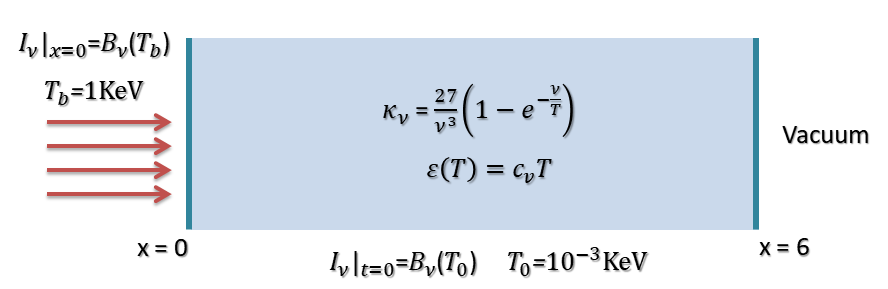
\includegraphics[width=0.75\textwidth]{FC_Test_1d.png}
		\caption{\label{fig:FC_Test_1d}
			Fleck and Cummings test problem}
	\end{figure}

	A 1D homogeneous slab is defined as 6 cm thick whose material opacity is given by
	\begin{equation}
		\varkappa_{\nu} = \frac{27}{\pr{h\nu}^3}\pr{1-e^{-\frac{h\nu}{kT}}}.
	\end{equation}
	
	The left boundary is subject to incoming radiation with black-body spectrum at temperature $T_b = 1$ keV and the right boundary is vacuum. The initial temperature of the slab is $T_0 =1$ eV, and the initial radiation distribution is given as the black-body spectrum at this temperature. This test approximates material energy density as a linear function of temperature
	\begin{equation}
		\varepsilon = \cv T,
	\end{equation}
	
	where the heat capacity of the material is given as
	\begin{equation}
		\cv = 0.5917\ar T_b^3.
	\end{equation}
	
	We use a uniform spatial mesh of 60 cells of length 0.1 cm, 17 energy groups and the double $S_4$ Gauss-Legendre quadrature set. Convergence criteria for temperature and energy density are $\epsilon_T=\epsilon_E=10^{-12}$. Fig. \ref{fig:ref_sols} displays the solution for temperature and total energy density for select instants of time obtained with the TRT problem by means of the MLQD method. Figure \ref{fig:ref_errs_inf_roms} presents the relative error of the solution of the $P_1$, $P_{\frac{1}{3}}$ and diffusion models to the MLQD solution in the $L_1$ norm. These models produce high errors at the early times of the problem and level off to a lower error once the steady state has been reached.
	
	%=================================================================================
	% TEST PROBLEM SOLUTIONS
	\begin{figure}[ht!]
		\centering
		\subfloat[Temperature \label{subfig:refcase_temp_sol}]{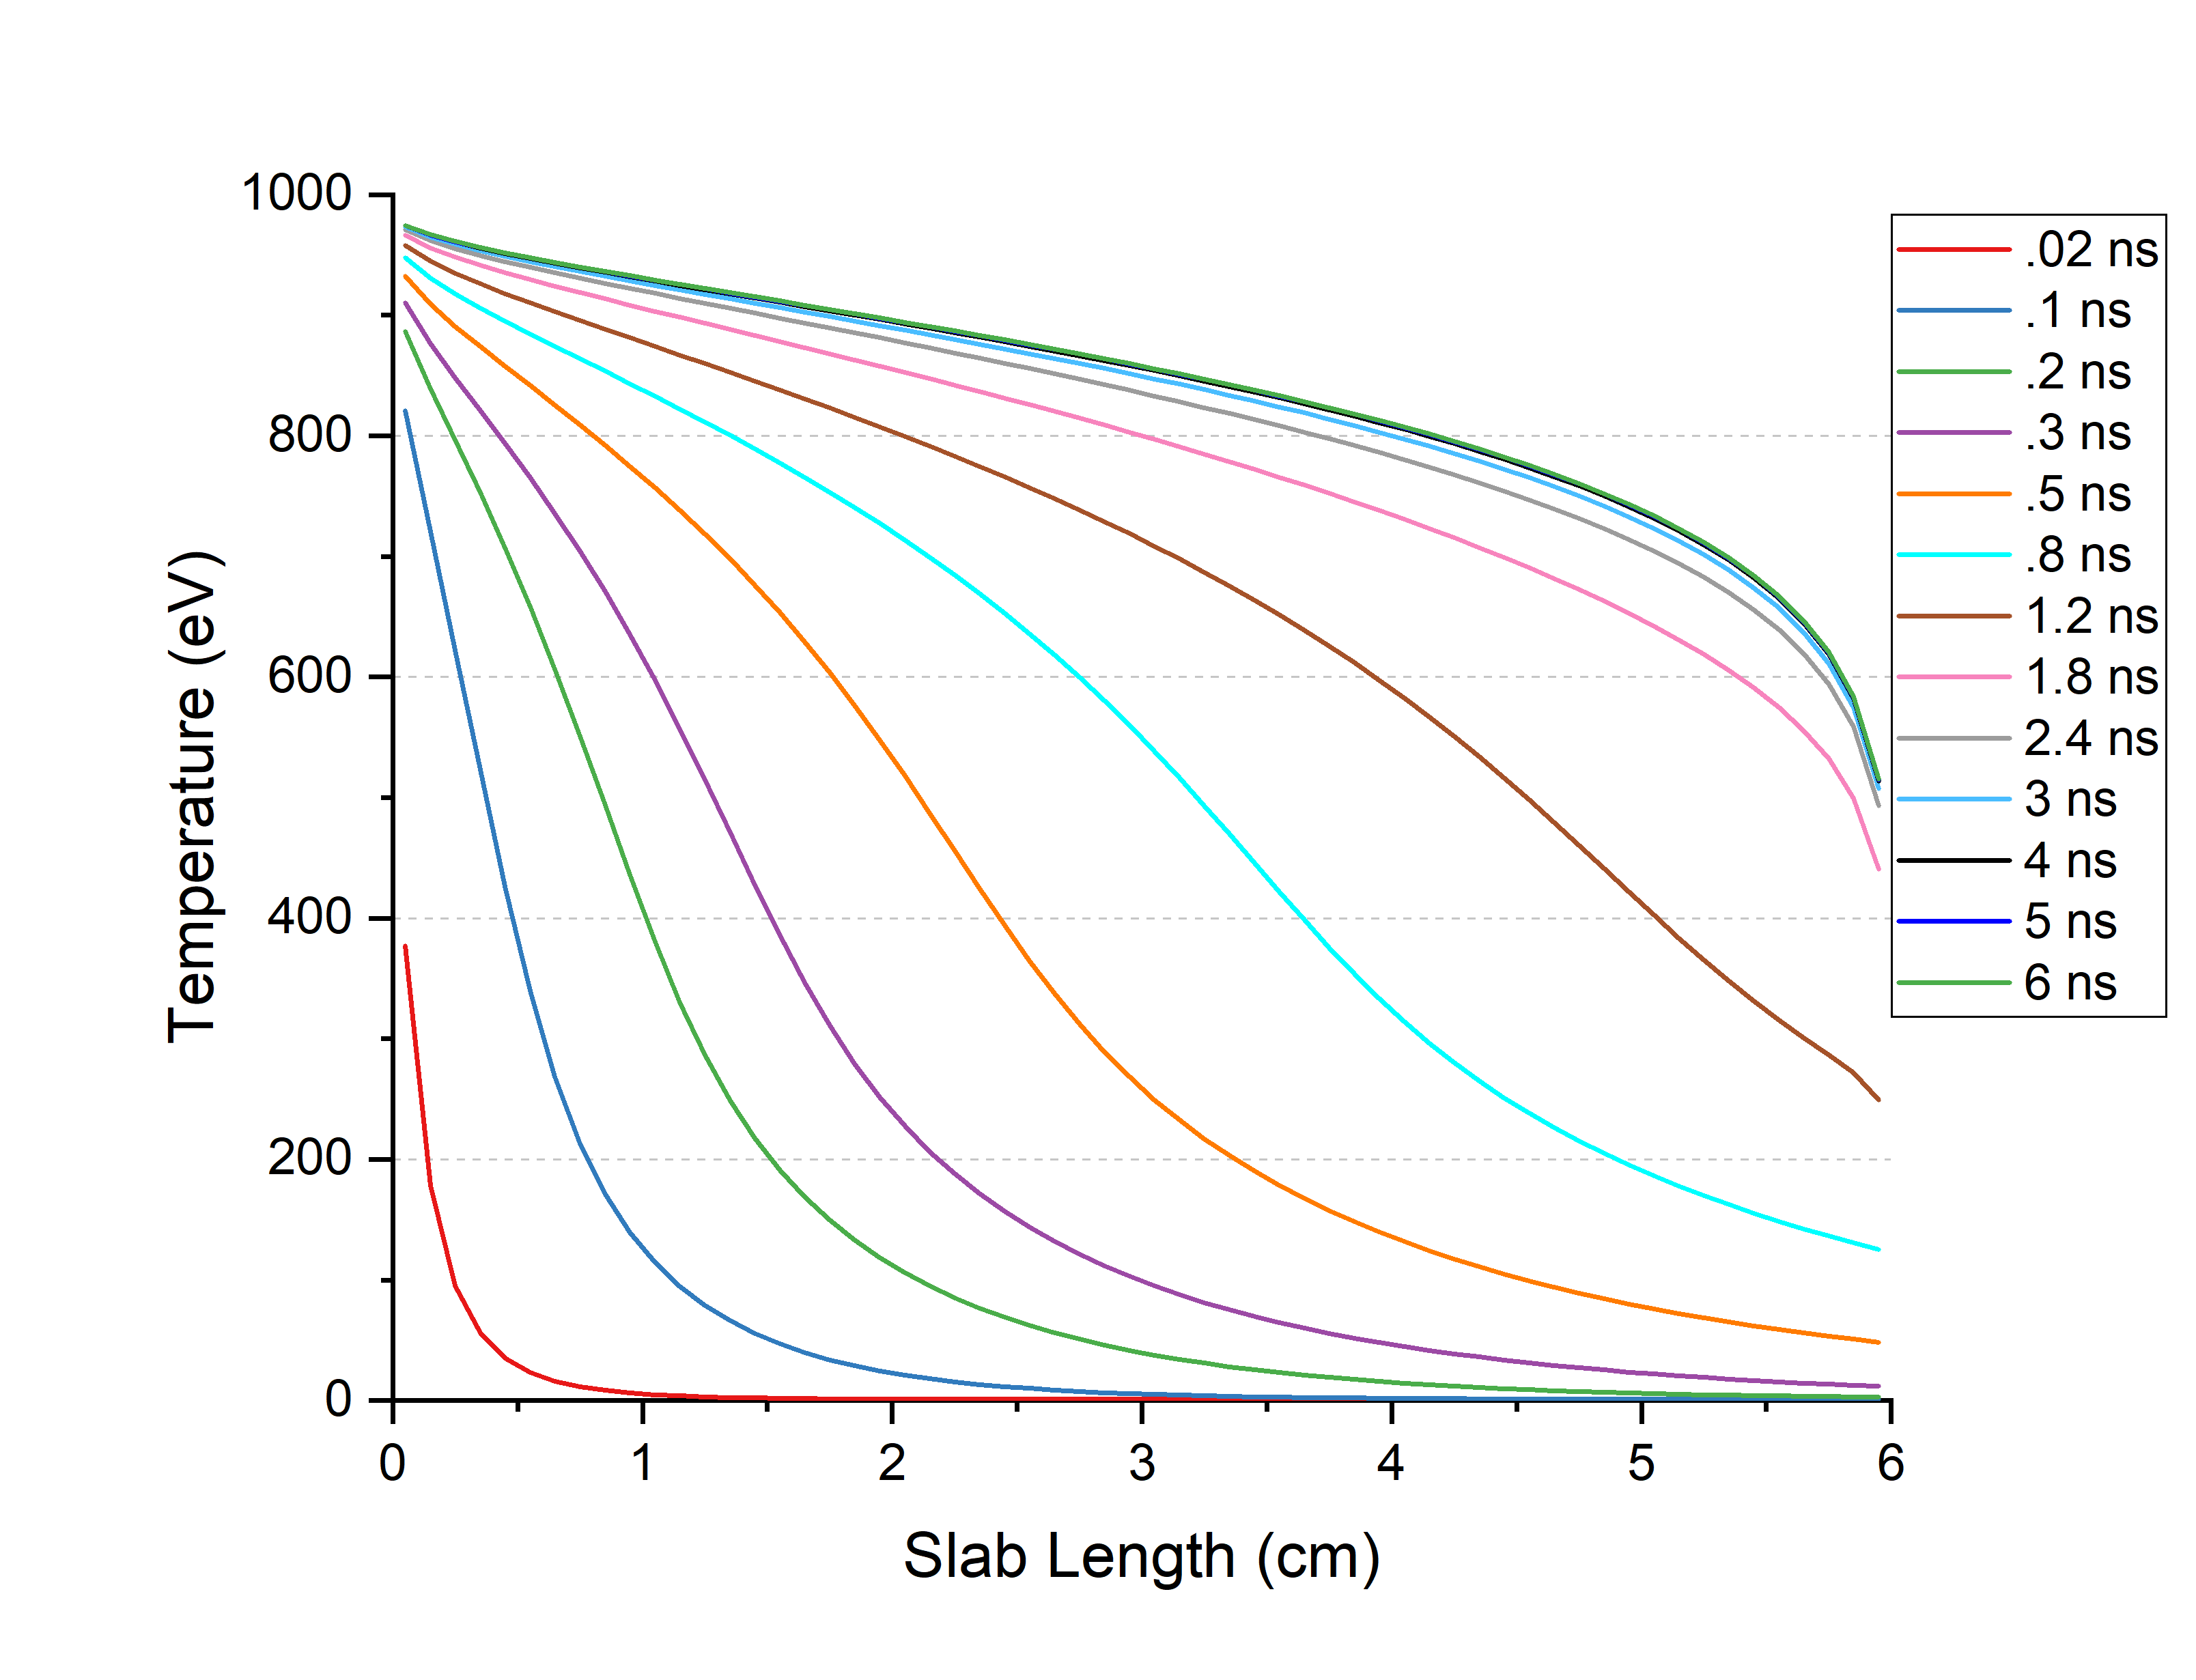
\includegraphics[width=0.5\textwidth]{refcase_temp_sol.png}}
		\subfloat[Total energy density \label{subfig:refcase_E_sol}]{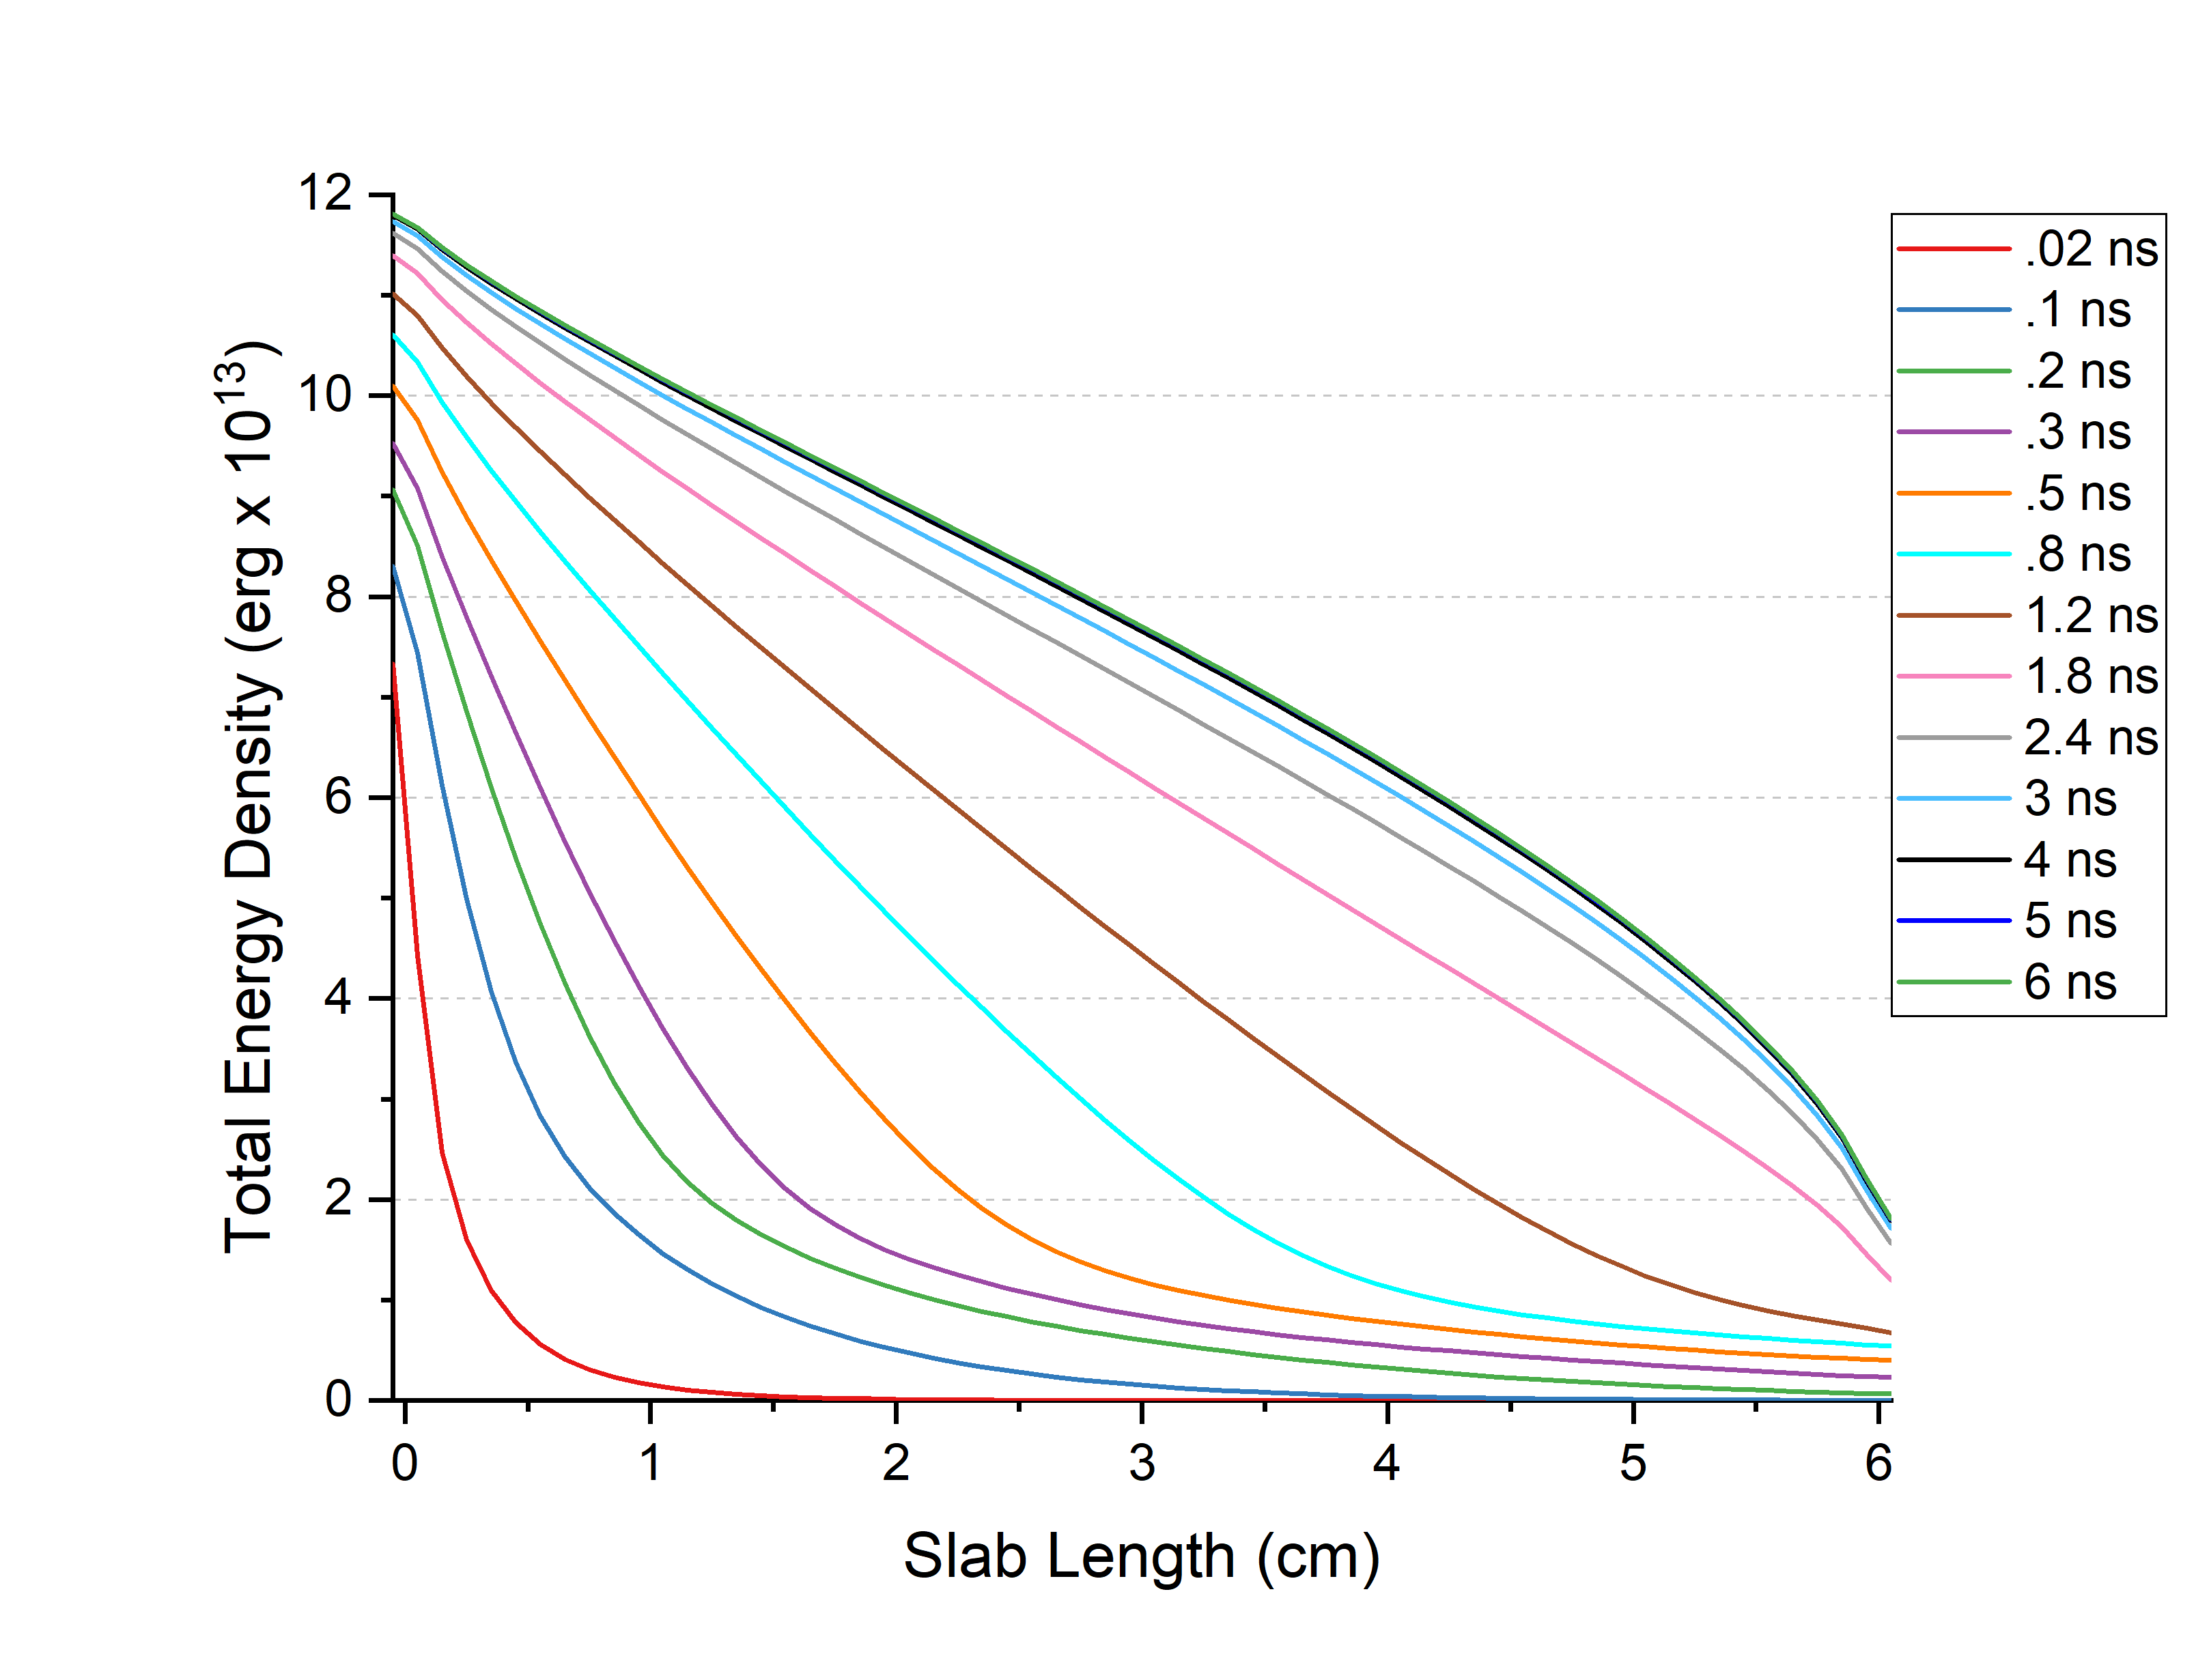
\includegraphics[width=0.5\textwidth]{refcase_E_sol.png}}
		\caption{\label{fig:ref_sols}
			RT solution obtained by the MLQD method to the F-C test problem.}
	\end{figure}

	%=================================================================================
	% TEST PROBLEM ERRORS
	\begin{figure}[ht!]
		\centering
		\subfloat[Temperature relative error \label{subfig:refcase_Temp_rel_inf_roms}]{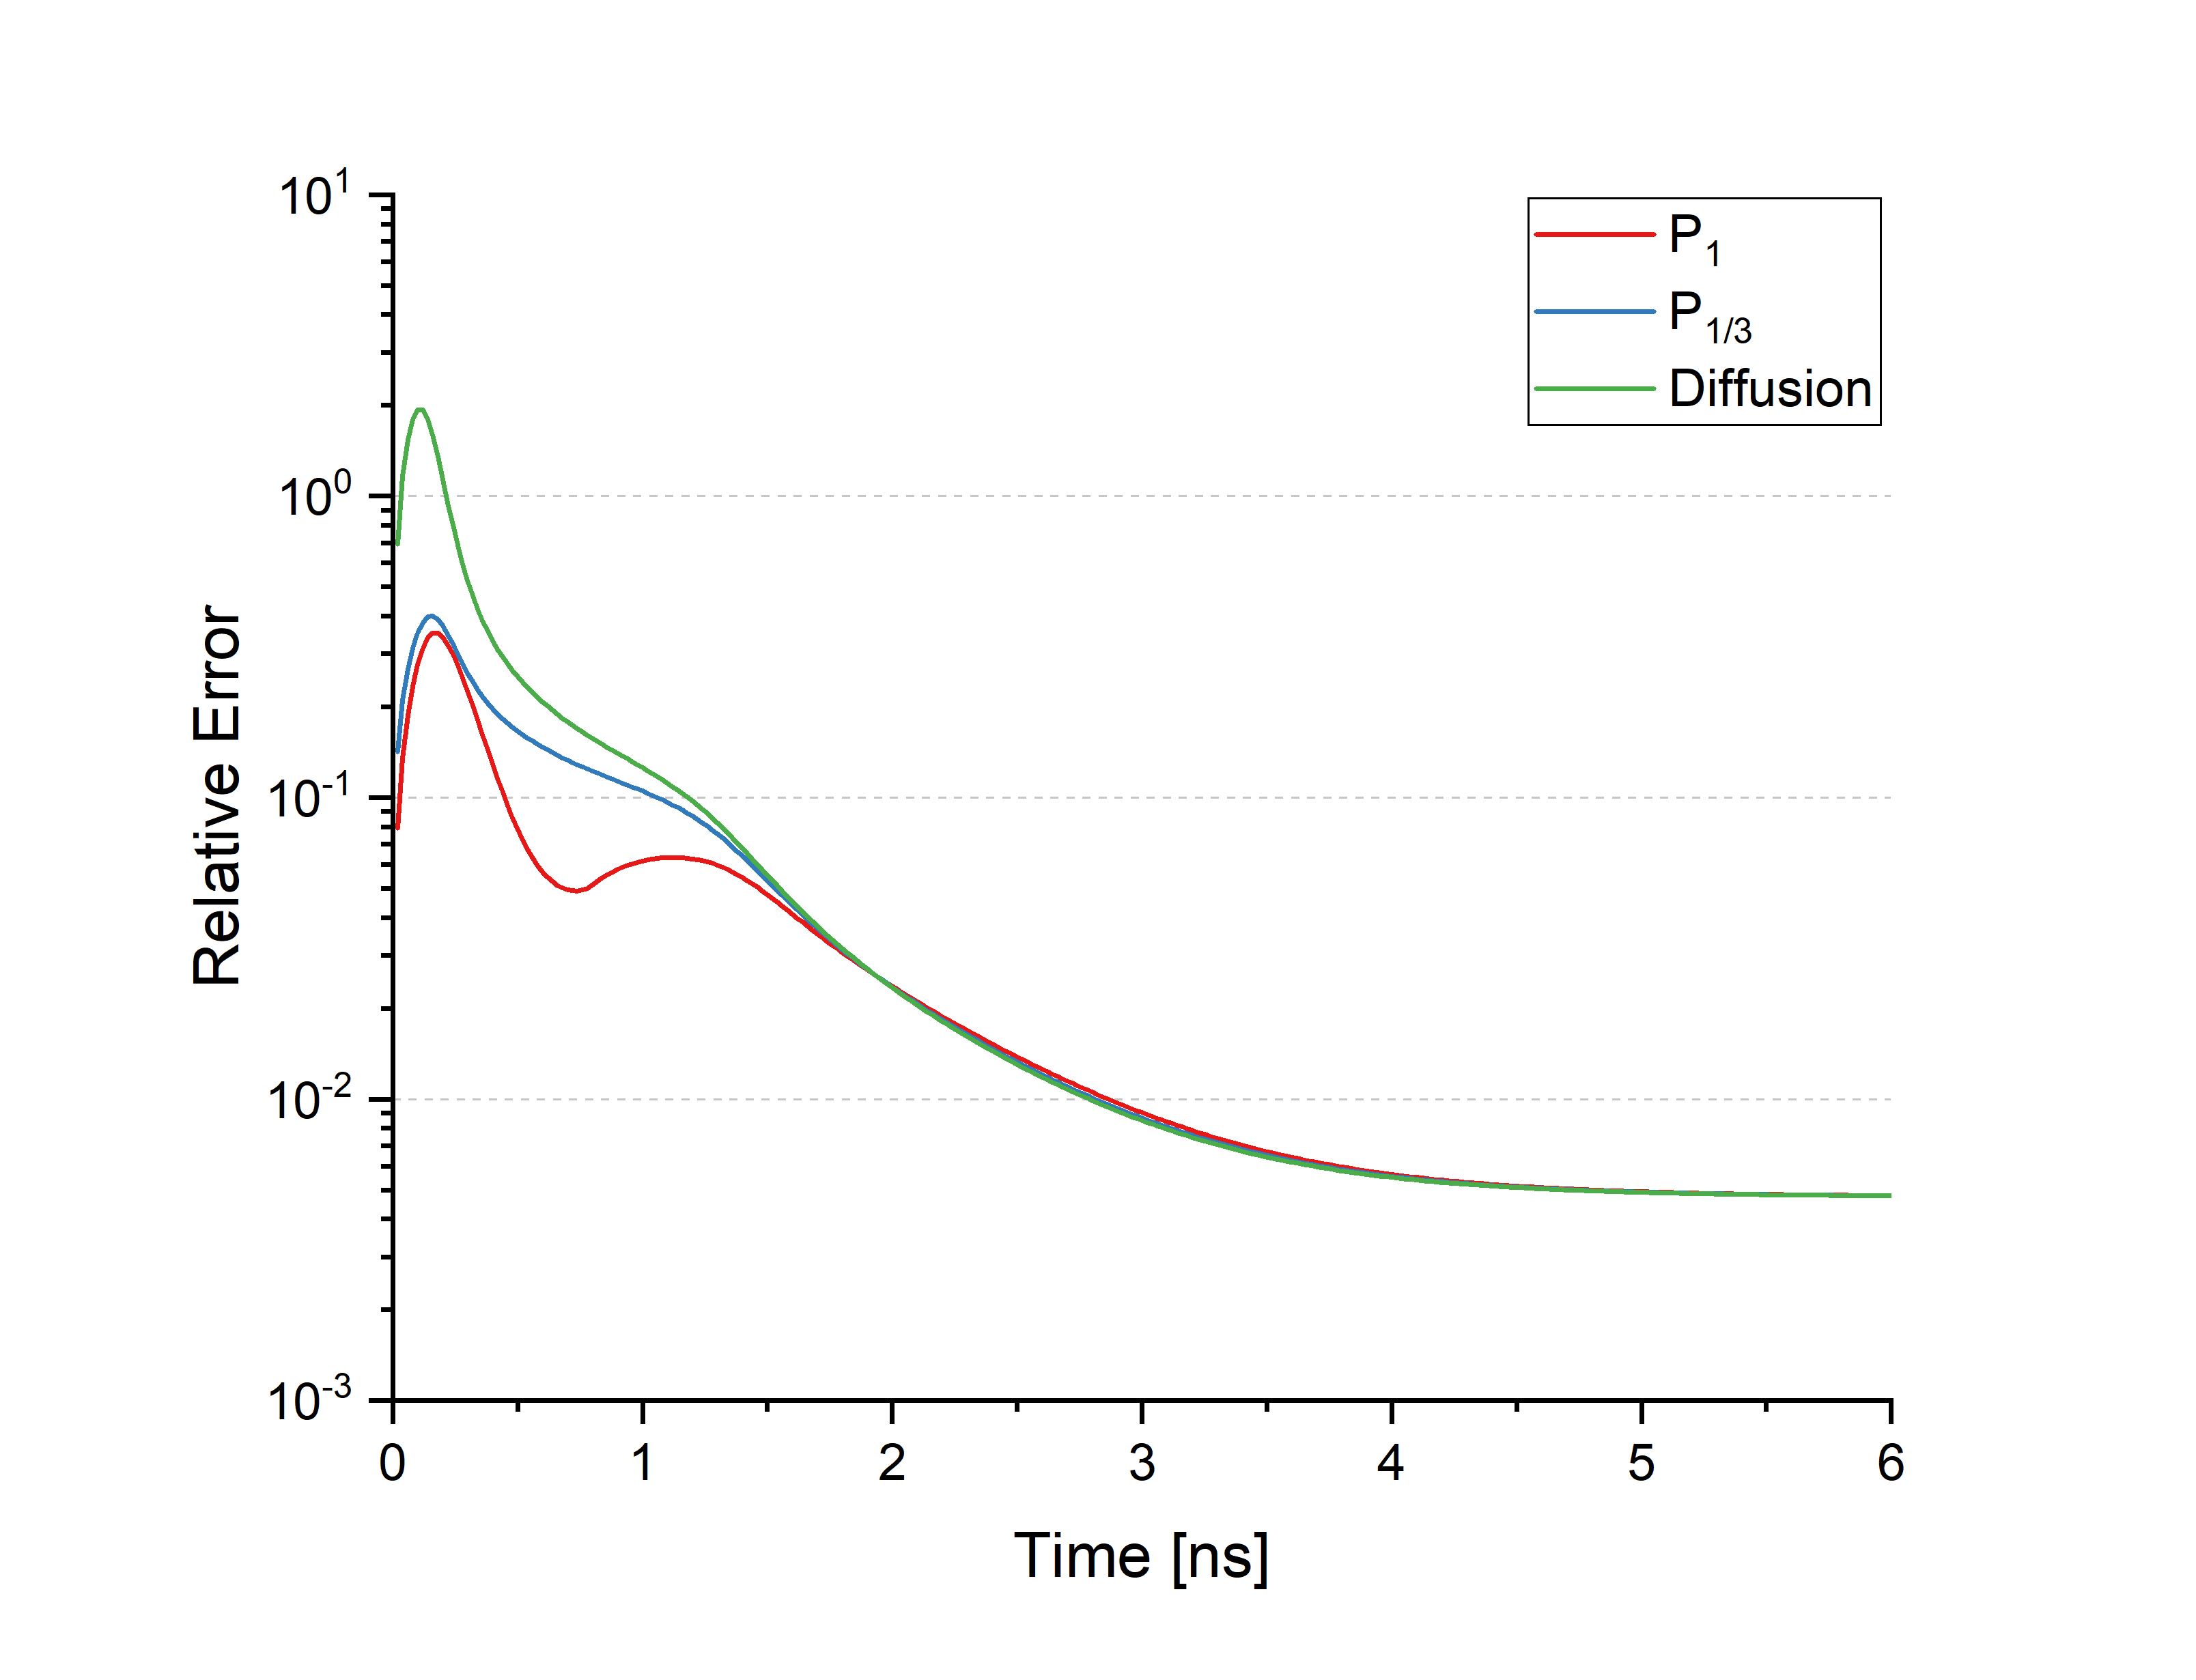
\includegraphics[width=0.5\textwidth]{refcase_Temp_rel_inf_roms.png}}
		\subfloat[Total energy density relative error \label{subfig:refcase_E_rel_inf_roms}]{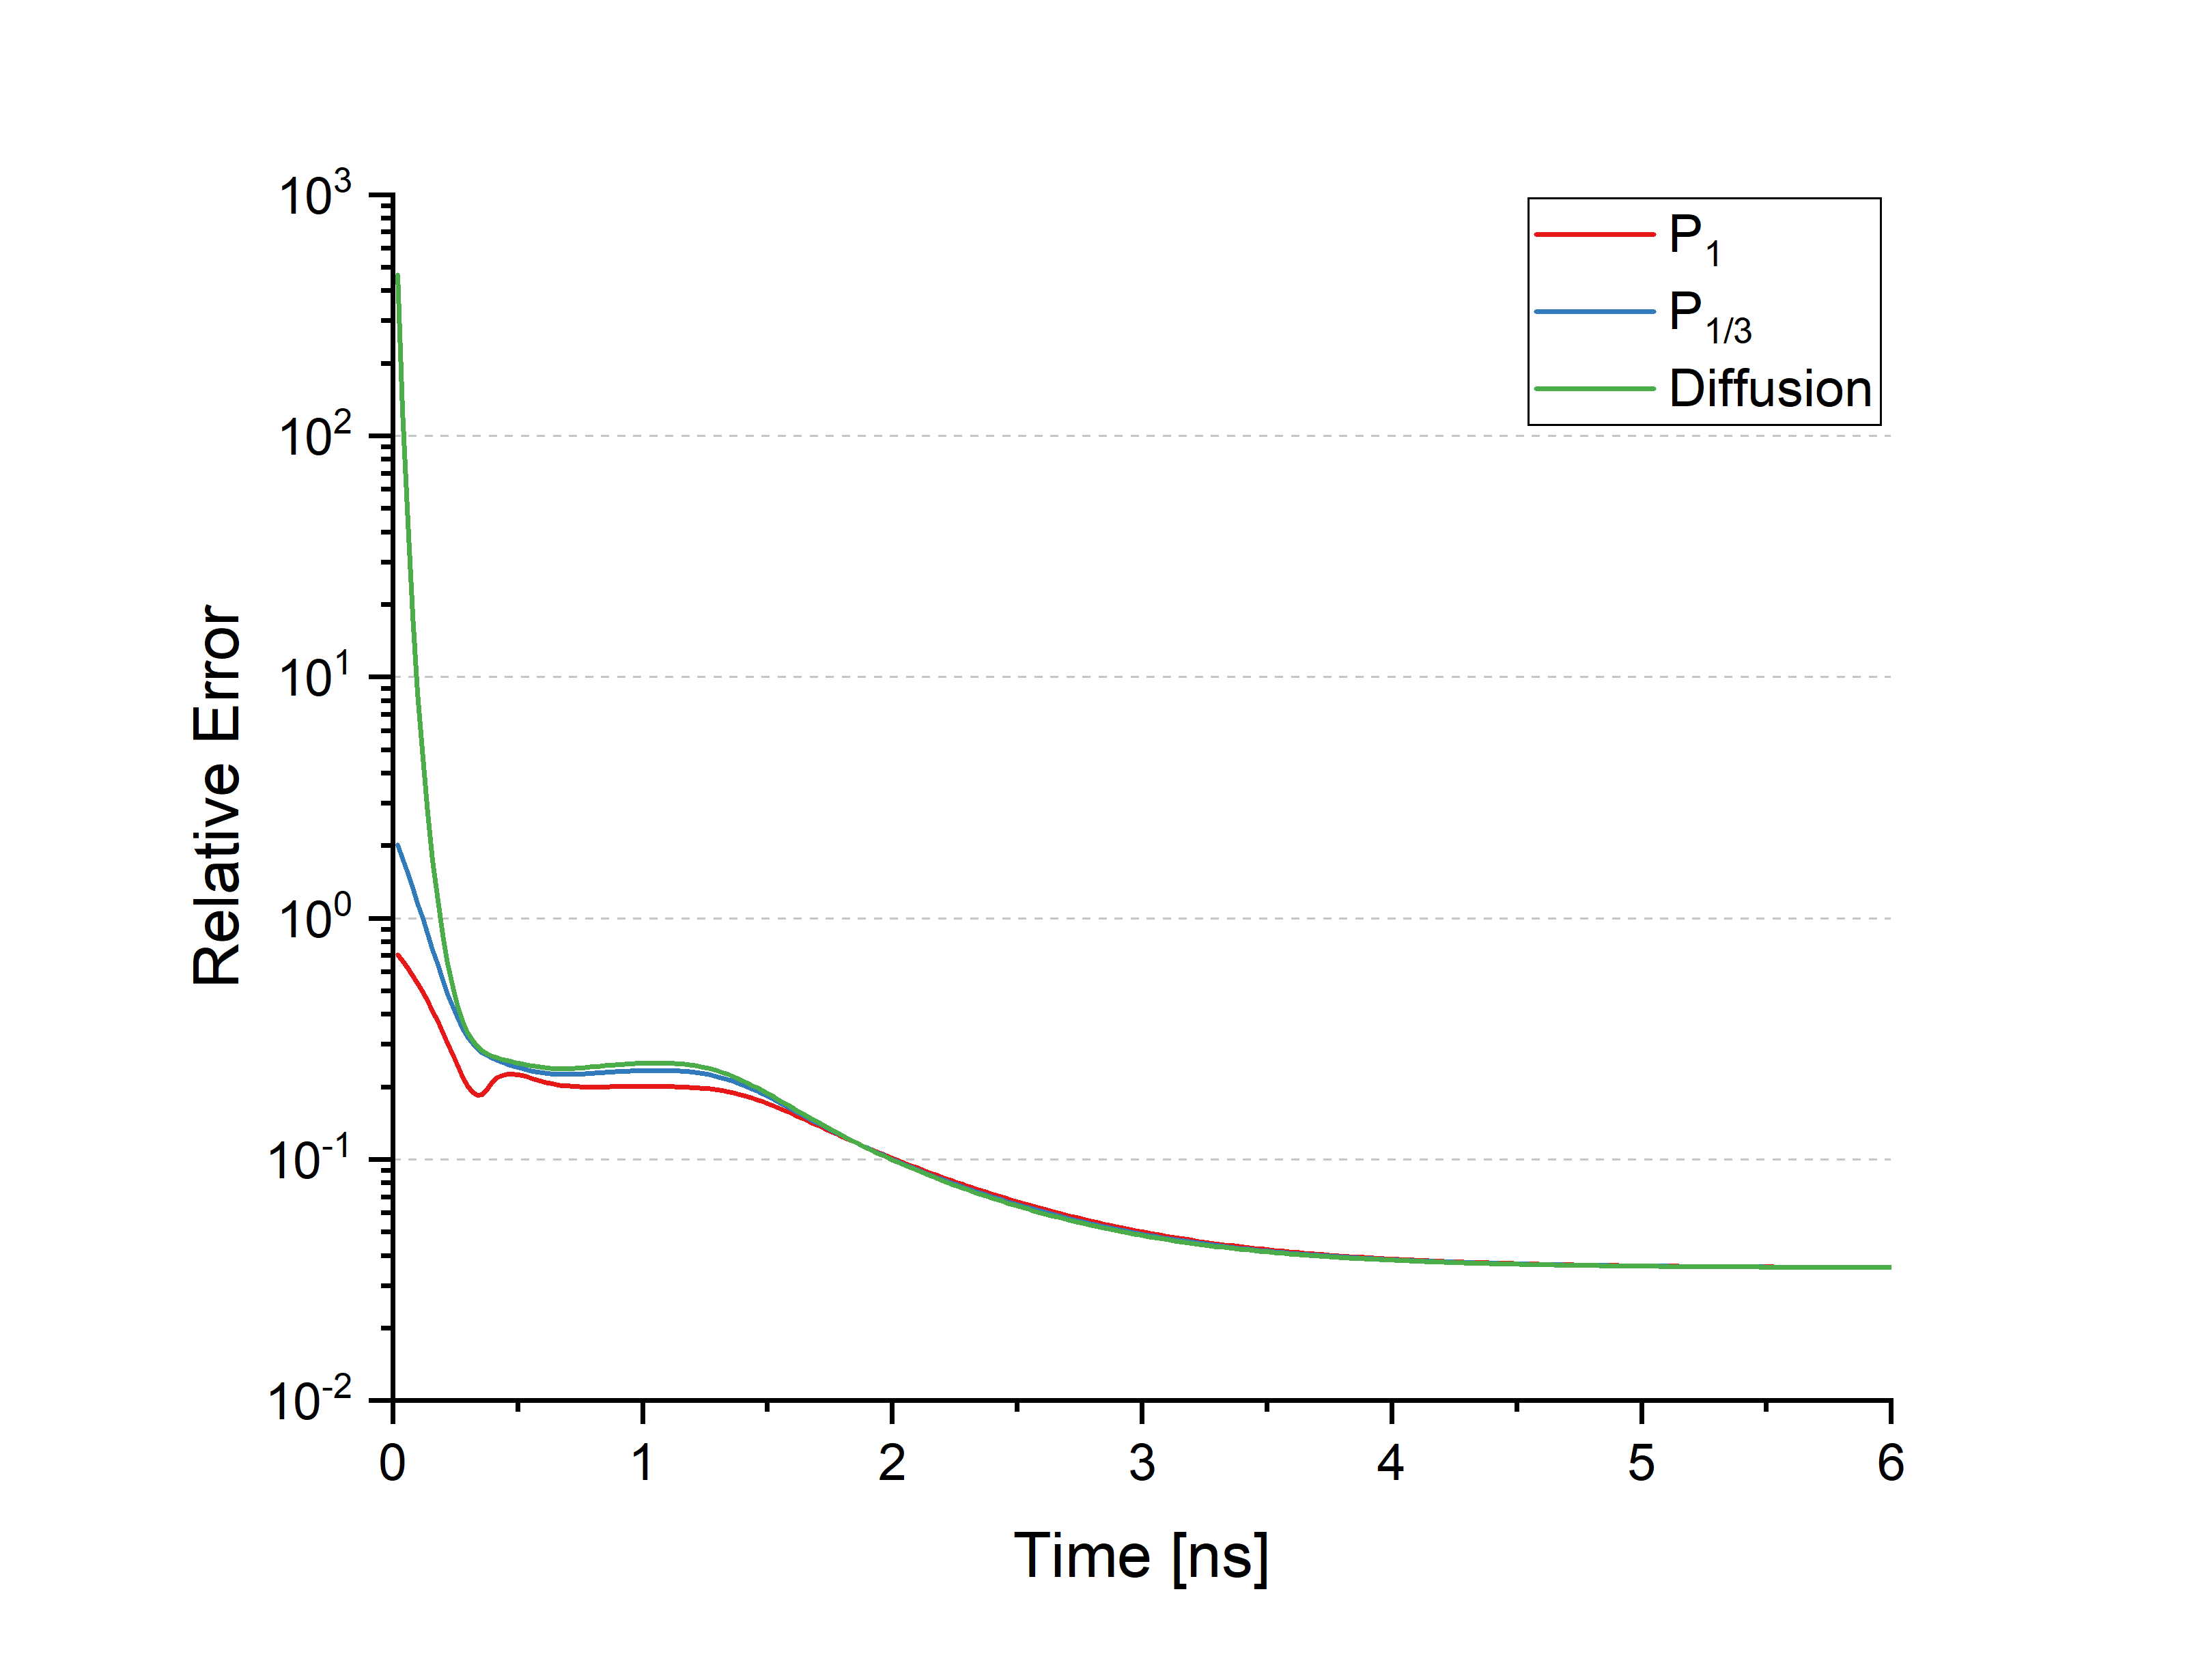
\includegraphics[width=0.5\textwidth]{refcase_E_rel_inf_roms.png}}
		\caption{\label{fig:ref_errs_inf_roms}
			Relative error of the $P_1$, $P_{\frac{1}{3}}$ \& Diffusion solution to the F-C test problem relative to the MLQD solution in $L_1$ norm}
	\end{figure}

\section{Low-Rank Approximation of Group QD Factors} \label{sec:reduced_qdf}
	%The first step in developing the MLOQD-POD ROM is to form a database of known group QD factors $\bA^f_g$. Given the solution to the F-C test problem, the reference group QD factors as a part of the solution of this TRT problem are known on some grid in phase space and time. The reference group QD factors are formed into $N_g$ matrices $\bA^f_g$ whose columns are the group $g$ QD factor solutions for each time step in chronological order. The truncated SVD of $\bA^f_g$ generates reduced rank approximations of the QD factors $\bA^{f*}_g$. 
	
	Fig. \ref{fig:QD_sval_summary} displays the normalized magnitudes and $1-\gamma_n$ \eqref{worth_gam} of the singular values of $\bA^f_g$ for different energy groups. Table \ref{tab:mqd_sigtab} displays the rank of approximation $(r_g)$ involved per energy group at different values of  $\varepsilon_\sigma$ \eqref{cutoff_eps}.
	
	\ind Since the test problem has 60 spatial cells the vector of cell-average QD factors in space has 62 values including 2 boundary values. When $\varepsilon_\sigma=10^{-12}$, the full-rank SVD is used. Note that group 2 uses a significantly higher rank SVD than any other energy group for large $\varepsilon_\sigma$.  This behavior can be explained with Fig. \ref{subfig:QD_svals}, which depicts the singular values normalized to the largest singular value for 7 sample energy groups $\pr{g=1,2,3,4,8,12,17}$. Group 2 is the only group to have two plateau regions, of which the first is high in value. This leads to high-order expansions in group 2 for even large $\varepsilon_\sigma$. The point where the singular values level off to a lower bound is smaller for each successive energy group excluding group 1.
	
	\ind Fig. \ref{subfig:inv_worths} displays $1-\gamma_n$ for each energy group and value of $n$ to show $\gamma_n$ of each successive reduced rank approximation of the QD factors per energy group. $1-\gamma_n$ is chosen over $\gamma_n$ for sake of clarity as it is much easier to analyze on a plot. Some of the latter energy groups quickly reach a value of $10^{-16}$ or numerically zero fairly early, as soon as $n=30$. As seen in Fig. \ref{subfig:QD_svals}, group 2 forms a unique shape among the other curves and demonstrates that significantly higher rank must be used compared to other groups to decrease the value of $1-\gamma_n$.

 	%=================================================================================
 	% SINGULAR VALUE FIGS
	\begin{figure}[ht!]
		\centering
		\subfloat[Normalized singular values of $\bA^f_g$ (QD factor database matrices) \label{subfig:QD_svals}]{\includegraphics[width=0.5\textwidth]{QD_svals.png}}
		\subfloat[$1-\gamma_n$ for $\bA^f_g$ (QD factor database matrices) \label{subfig:inv_worths}]{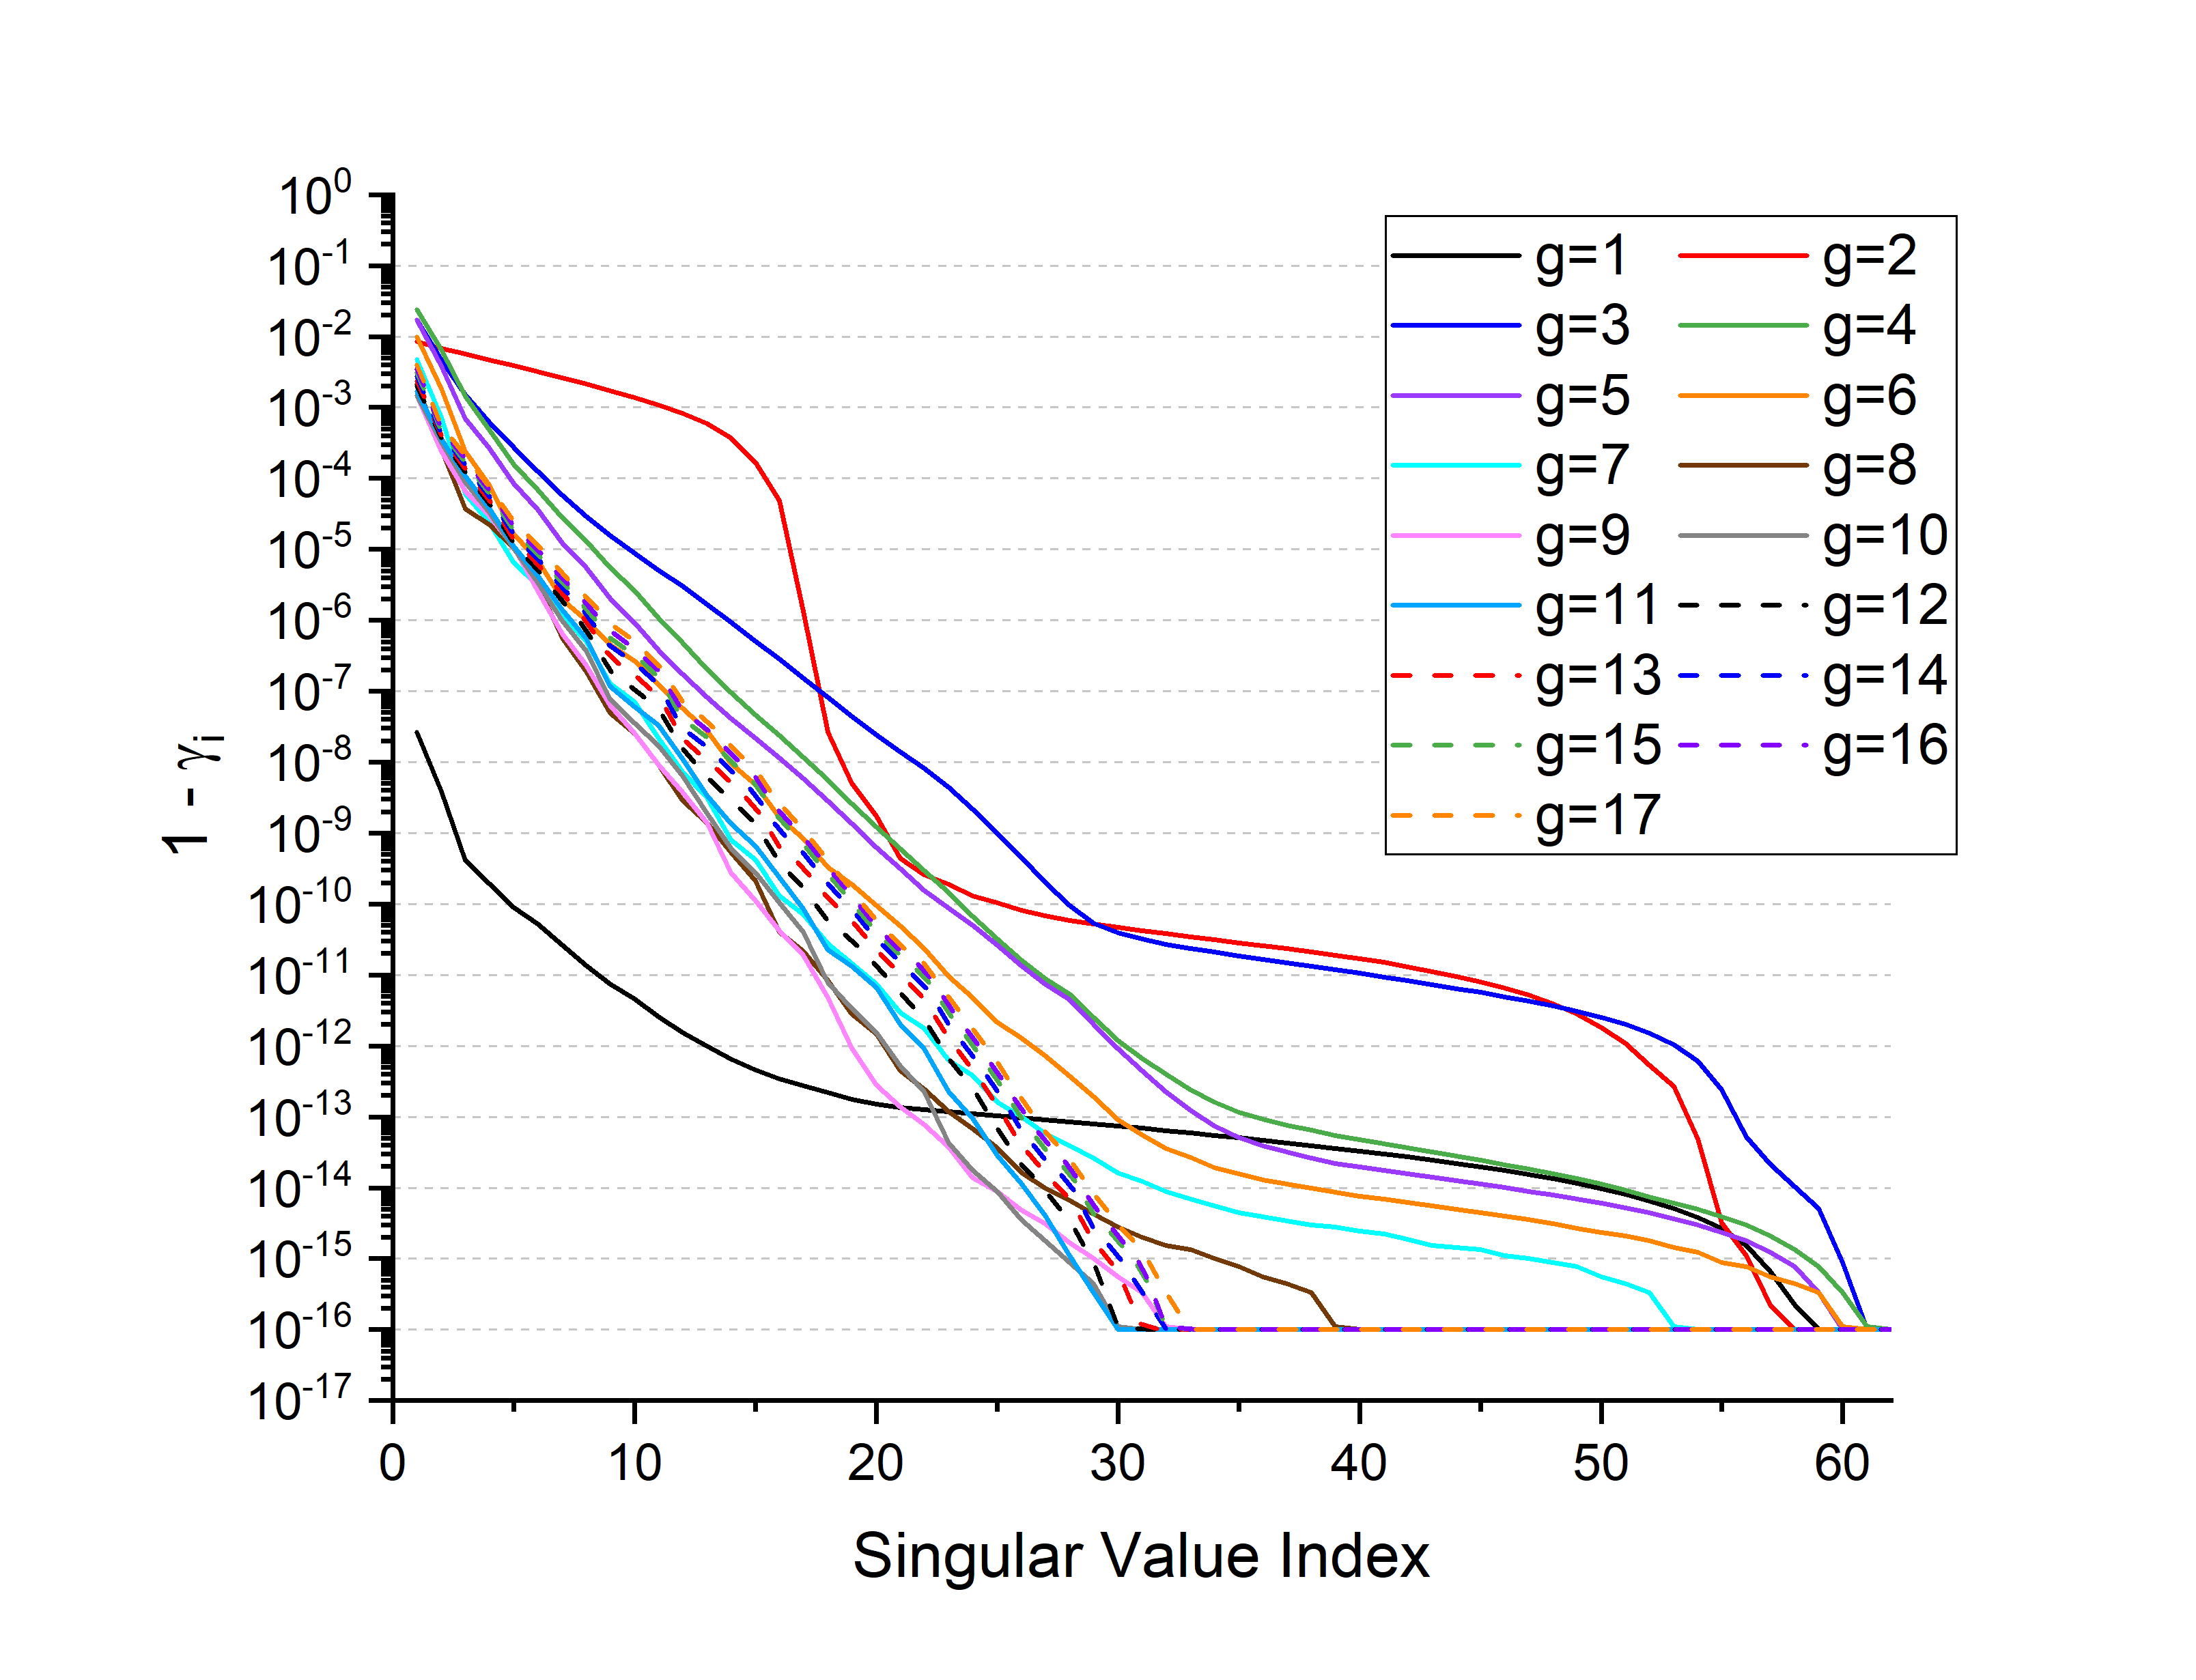
\includegraphics[width=0.5\textwidth]{inv_worths.png}}
		\caption{\label{fig:QD_sval_summary}
			Group QD factor normalized singular values and $1-\gamma_n$}
	\end{figure}
	
	%=================================================================================
	% SINGULAR VALUE TABLE
	\begin{table}[ht!]
		\caption{	\label{tab:mqd_sigtab} The rank of approximation $(r_g)$ of $f_g$ in each energy group for decreasing values of $\varepsilon_\sigma$}
		\begin{tabular}{|c||c|c|c|c|c|c|c|c|c|c|c|c|c|c|c|c|c|}	
			\hline
			$\varepsilon_\sigma \backslash  \ g$ & 1 & 2 & 3 & 4 & 5 & 6 & 7 & 8 & 9 & 10 & 11 & 12 & 13 & 14 & 15 & 16 & 17 \\
			\hline
			\hline
			$10^{-1}$ & 1  &  1 & 2  & 2  & 2  & 1  &  1 & 1 &  1 &   1 & 1 &  1 &  1 & 1 &  1 &  1 & 1 \\ \hline
			$10^{-2}$ & 1 & 16 & 6 & 5 & 5 & 4 & 3 & 3 & 3 & 3 & 3 & 3 & 3 & 4 & 4 & 4 & 4\\ \hline
			$10^{-3}$ & 1 & 18 & 13 & 11 & 10 & 7 & 7 & 7 & 7 & 7 & 7 & 8 & 8 & 8 & 8 & 9 & 9\\ \hline
			$10^{-4}$ & 2 & 19 & 21 & 17 & 16 & 14 & 12 & 11 & 11 & 12 & 12 & 12 & 13 & 13 & 14 & 14 & 14\\ \hline
			$10^{-12}$ & 62 & 62 & 62 & 62 & 62 & 62 & 62 & 62 & 62 & 62 & 62 & 62 & 62 & 62 & 62 & 62 & 62\\ \hline
		\end{tabular}
	\end{table}

	
	\ind To investigate the causes for the results shown in Fig. \ref{fig:QD_sval_summary} and Table \ref{tab:mqd_sigtab} we observe the actual reduced rank forms of the QD factors. Select energy groups $g=\pr{2,3,8}$ are chosen as groups 2 and 3 require the highest ranks for large $\varepsilon_\sigma$, and group 8 is a good representative energy group for the rest of the group QD factors. Figs. \ref{fig:qdf_g2_recomps}, \ref{fig:qdf_g3_recomps} and \ref{fig:qdf_g8_recomps} show the low-rank approximations of the group QD factors $f_g^*$ for groups 2, 3 and 8 respectively. Each of these figures displays the approximate QD factors obtained for 6 different ranks $r=\pr{1,2,5,10,15,20}$. These figures show more clearly the reason for groups 2 and 3 being the most difficult to approximate with low rank. For all plots shown when r = 20 are used $\pr{r=20}$, the structure of the approximate QD factors has converged to the high order MLQD solution to the resolution of the plot.
	
	\ind For groups 2 and 3 the approximate QD factors are structured as a fast moving wave during the initial stage of the TRT problem that is related to the propagation of the radiation front in these energy groups that are optically thick at this stage. Group 8 shows a smoother wave structure because photons in this more optically thin group move faster through the spatial domain. The structure of the group 2 approximate QD factors is unique due to the discontinuous nature of the waves. They display a sharp drop at the end of each wave dropping to a value of 1/3. Since this must then be propagated from the left boundary to the right, an SVD of higher rank is required to recreate this structure with its sharp discontinuities. Thus Fig. \ref{fig:qdf_g2_recomps} shows the reduced rank forms of the group 2 approximate QD factors taking on a poor representation of the full rank form until at least $r=15$.
	
	\ind In Fig. \ref{fig:qdf_g3_recomps}, the group 3 approximate QD factors have converged to the resolution of the plot by the time the SVD with $r=15$ has been used, and most of the full rank form has been recreated with $r=10$. The group 8 approximate QD factors require an SVD of even smaller rank for the same accuracy, having converged to the full rank form by the resolution of the plot of Fig. \ref{fig:qdf_g8_recomps} for $r=10$. Using an SVD with $r=5$ for the approximate QD factors in group 8 also gives a very similar structure.

	%=================================================================================
	% QDF G2 RECOMP
	\begin{figure}[ht!]
		\centering
		\subfloat[r = 1 \label{subfig:qdf_g2_cut1}]{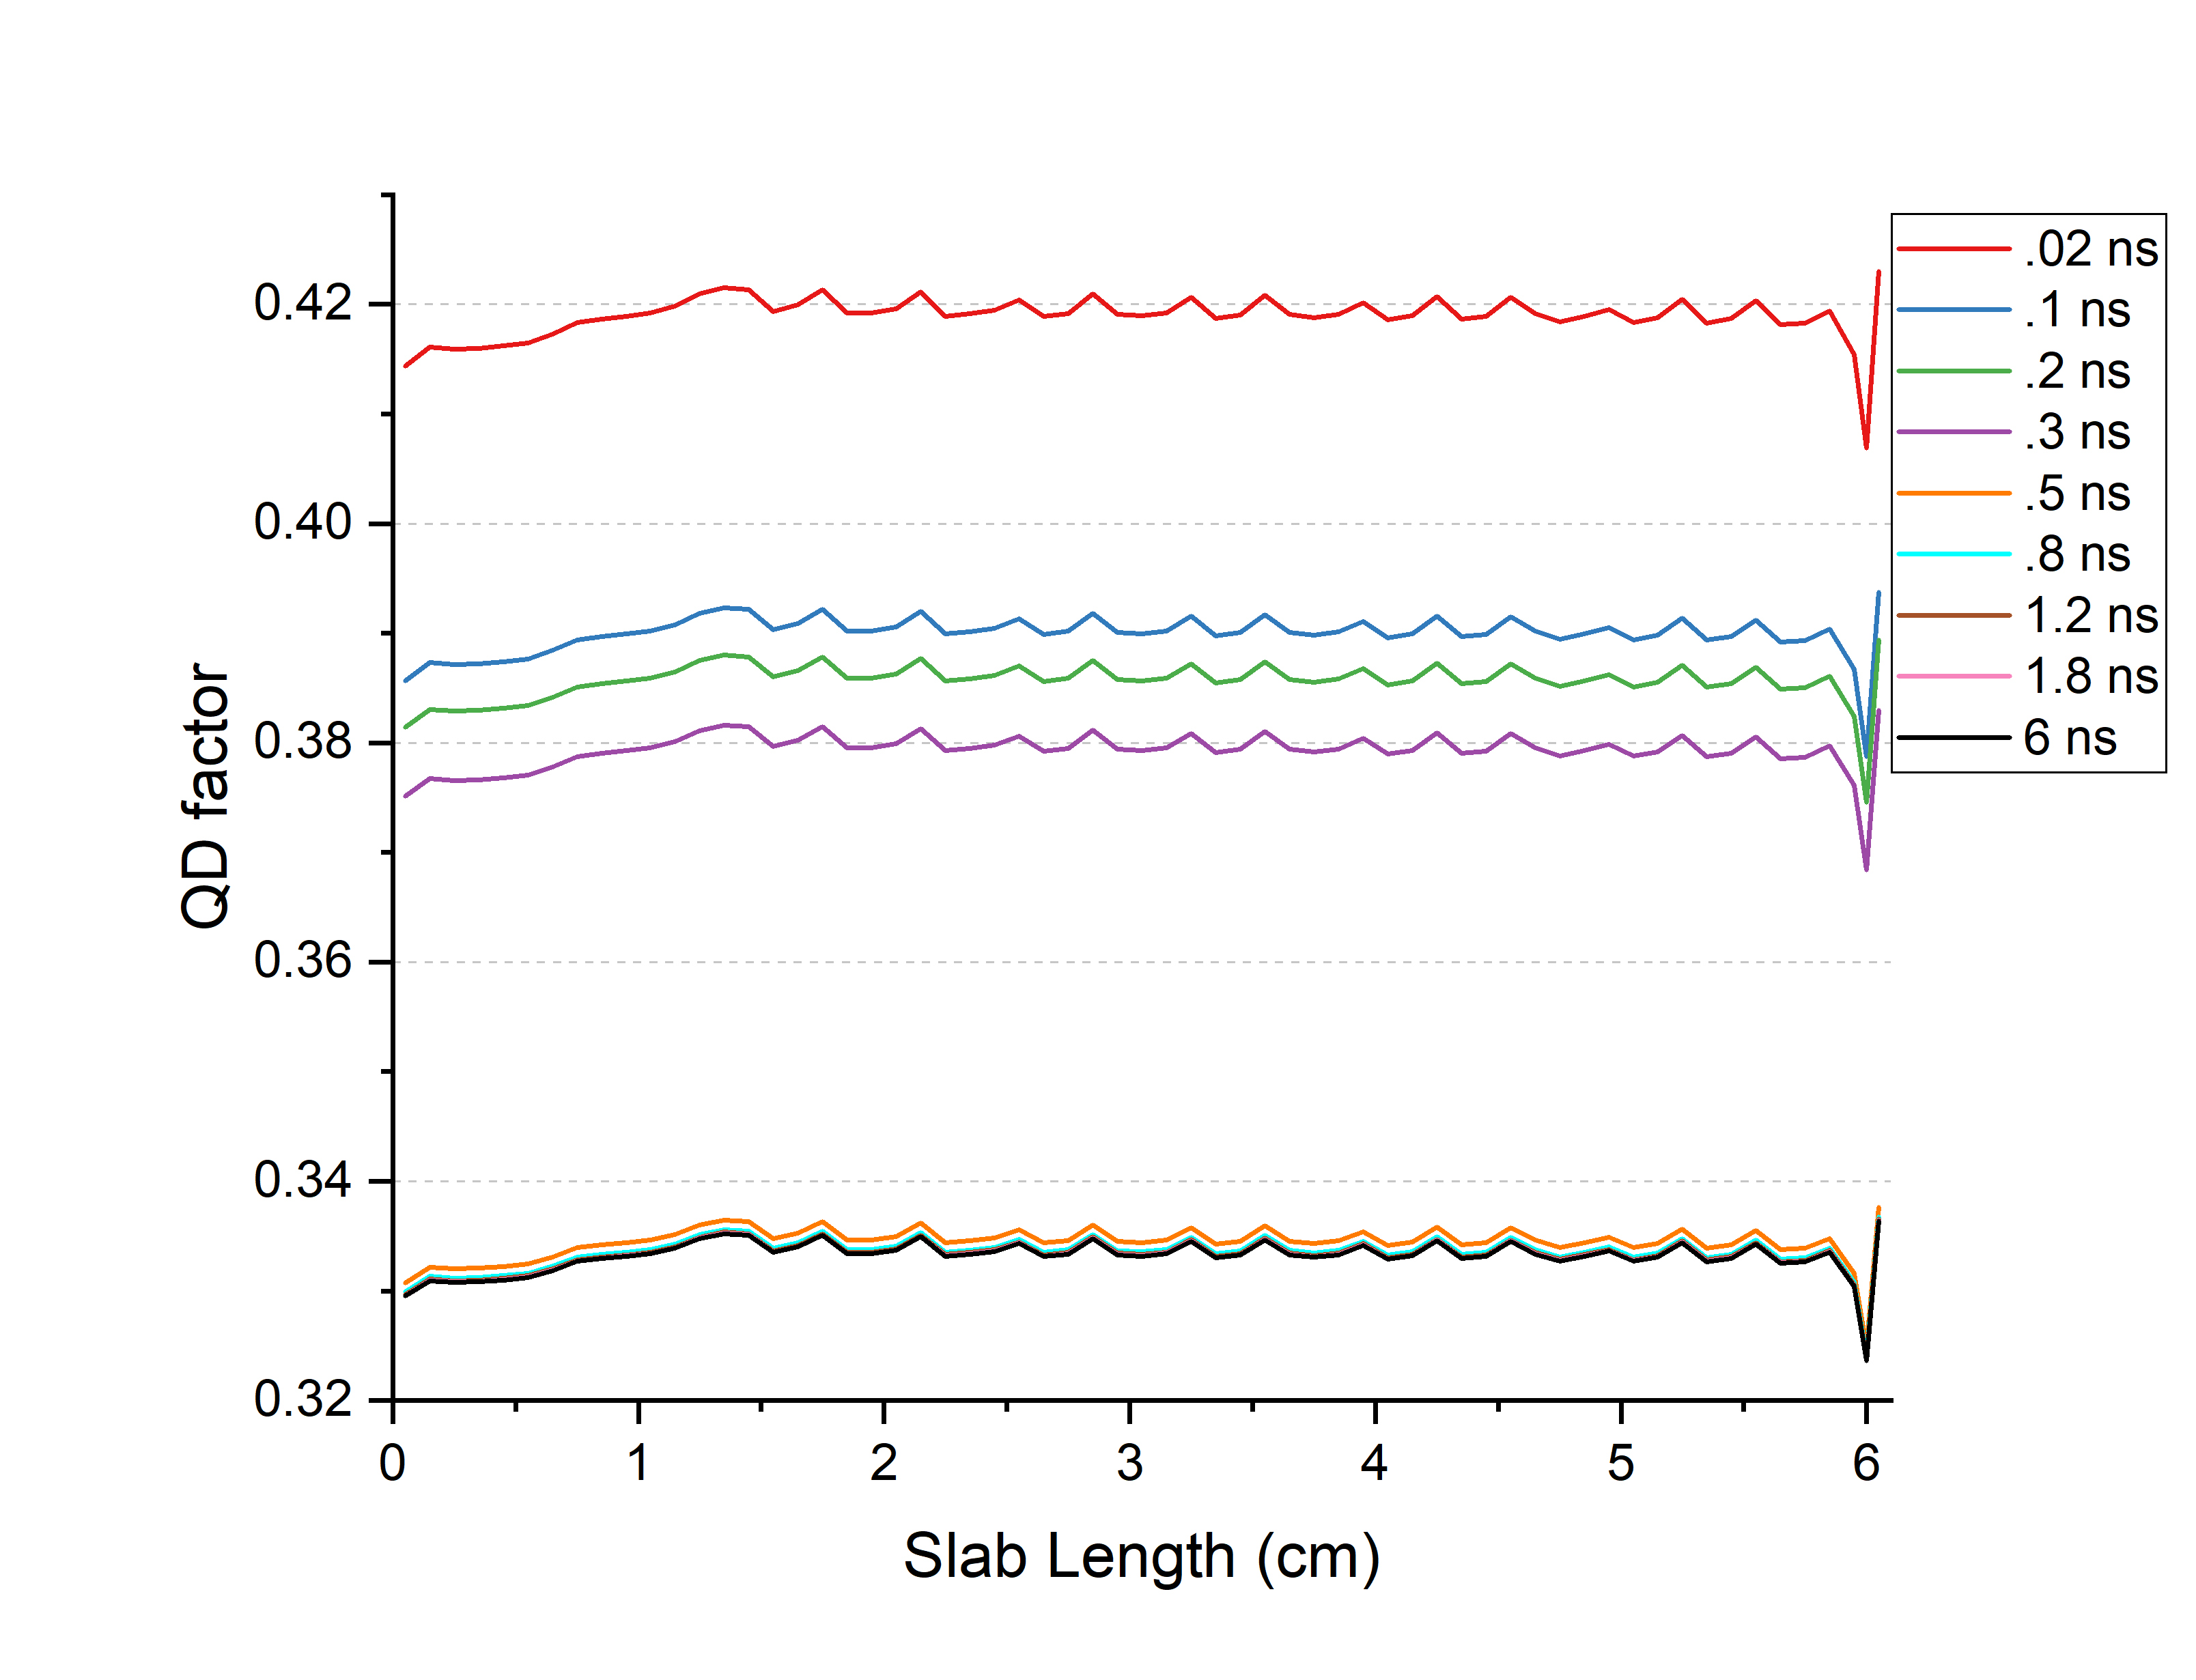
\includegraphics[width=0.5\textwidth]{qdf_g2_cut1.png}}
		\subfloat[r = 2 \label{subfig:qdf_g2_cut2}]{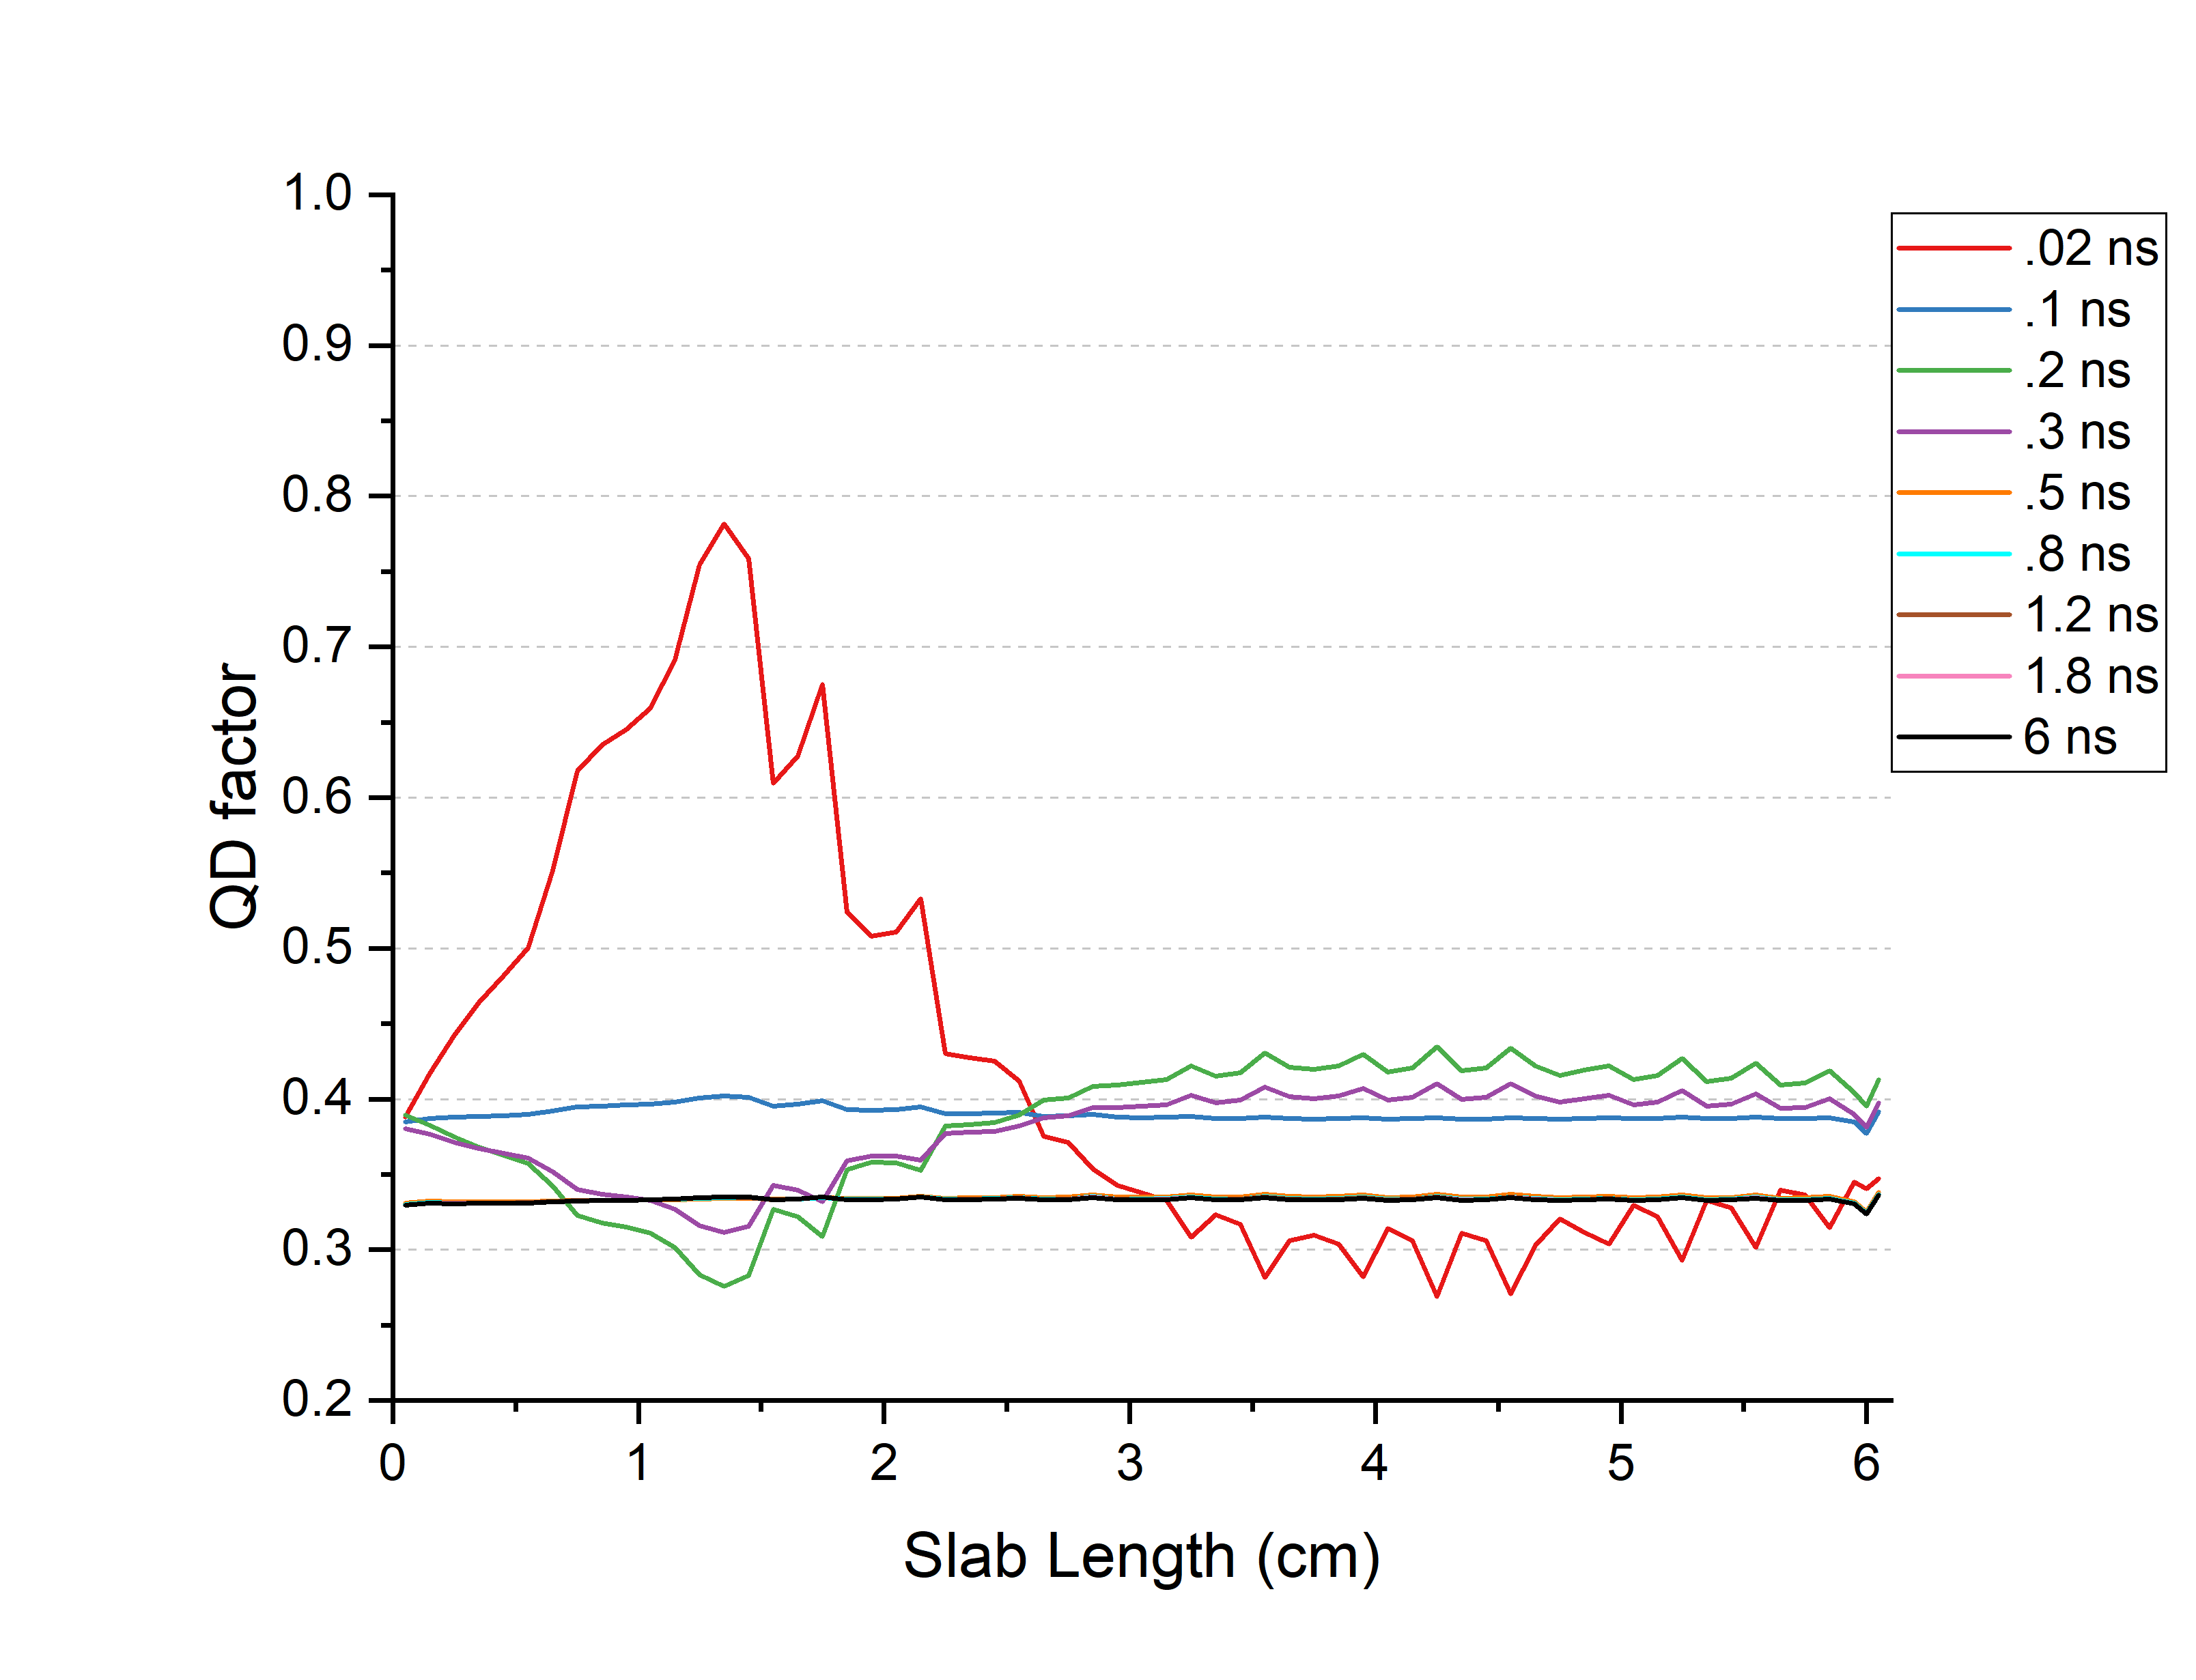
\includegraphics[width=0.5\textwidth]{qdf_g2_cut2.png}}\\
		\subfloat[r = 5 \label{subfig:qdf_g2_cut5}]{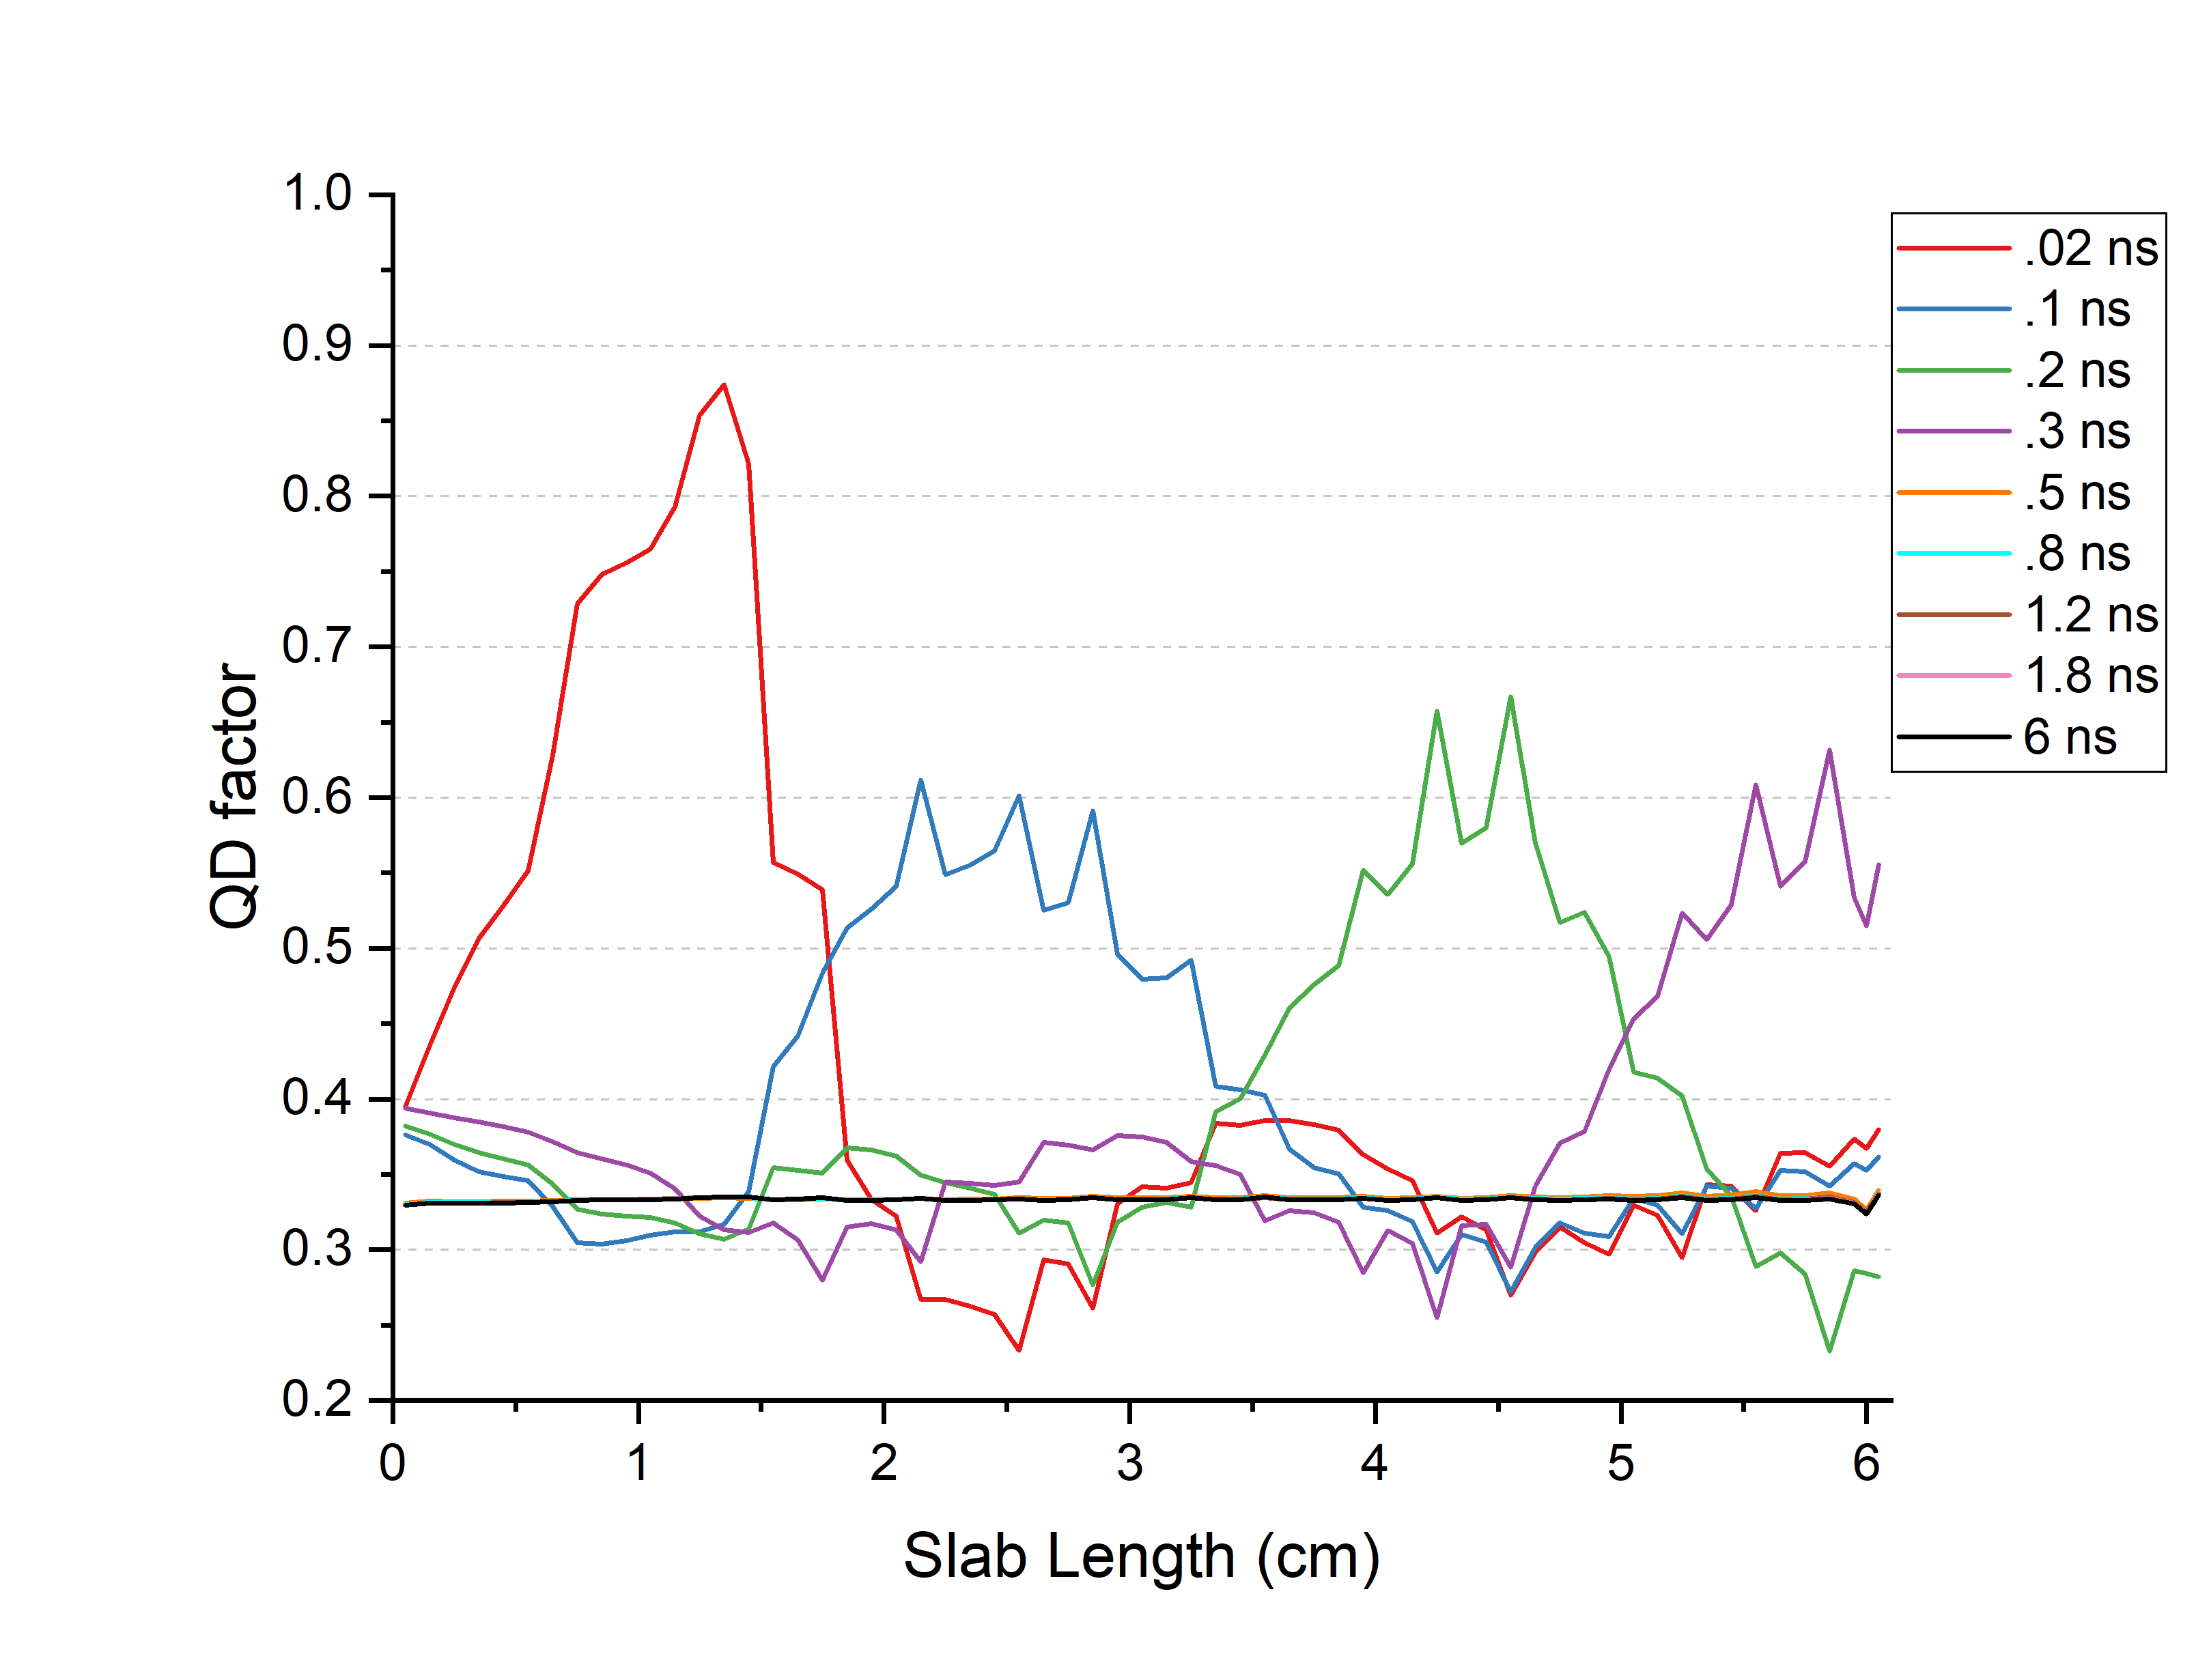
\includegraphics[width=0.5\textwidth]{qdf_g2_cut5.png}}
		\subfloat[r = 10 \label{subfig:qdf_g2_cut10}]{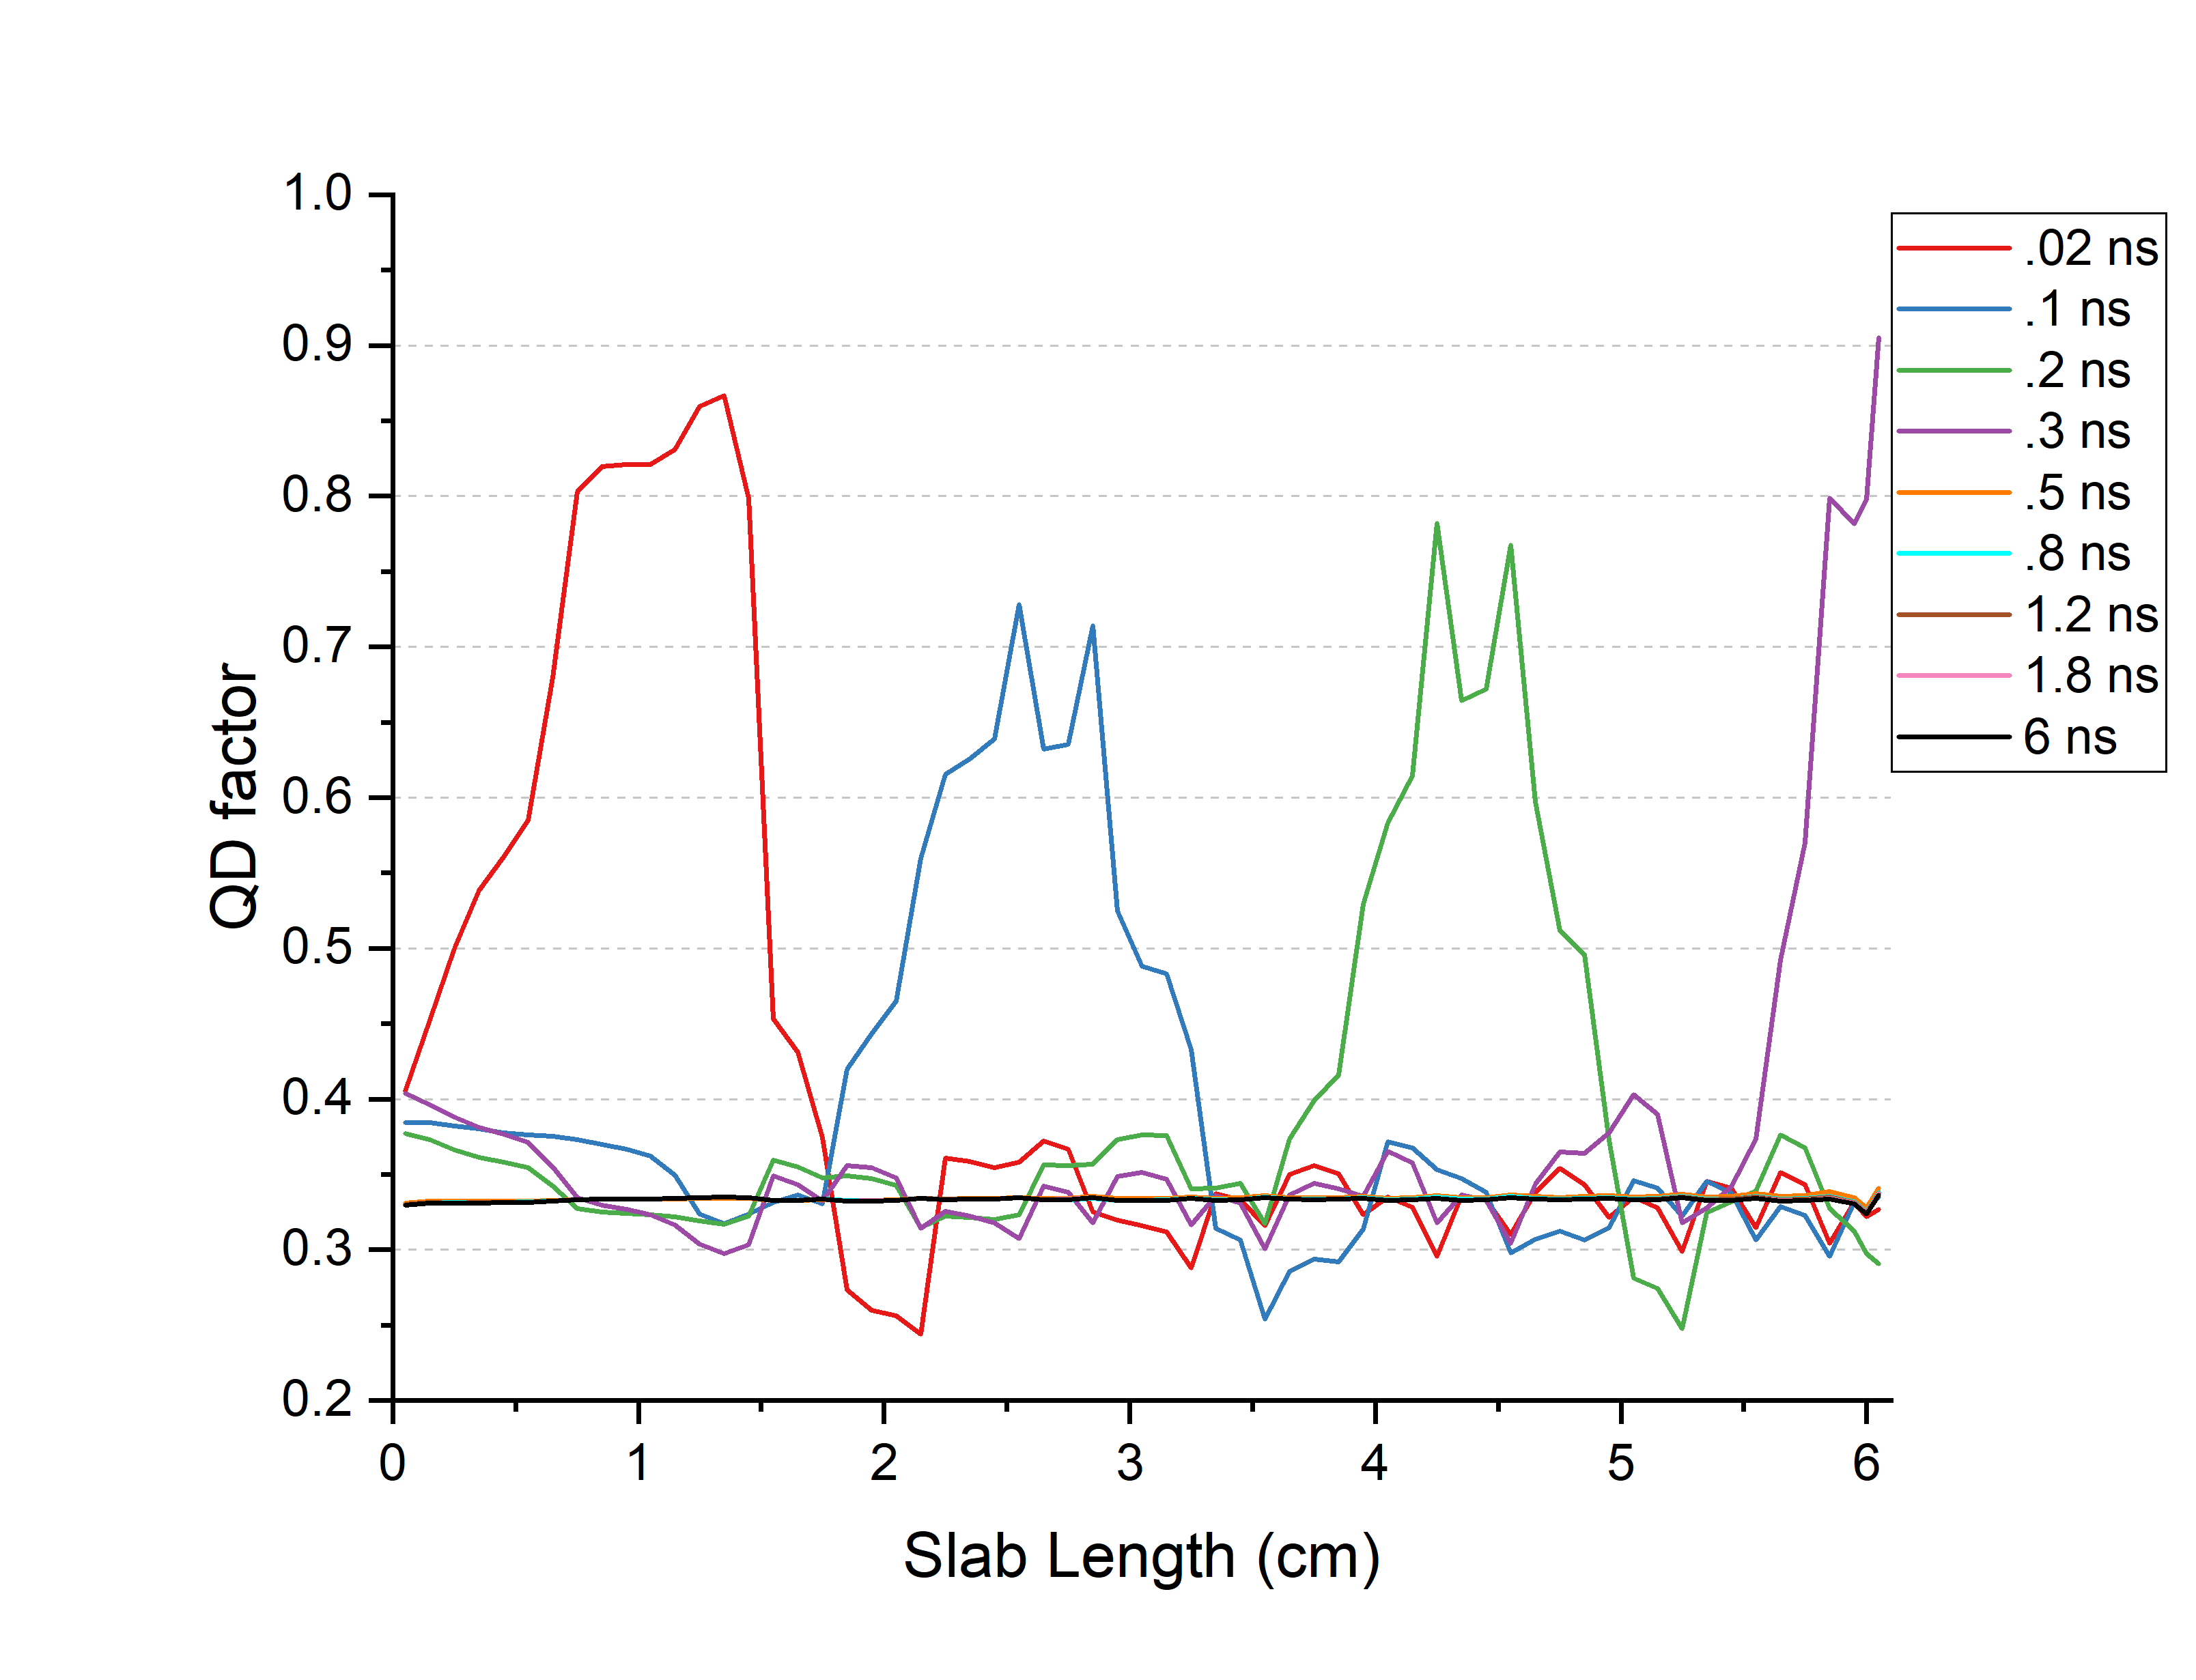
\includegraphics[width=0.5\textwidth]{qdf_g2_cut10.png}}\\
		\subfloat[r = 15 \label{subfig:qdf_g2_cut15}]{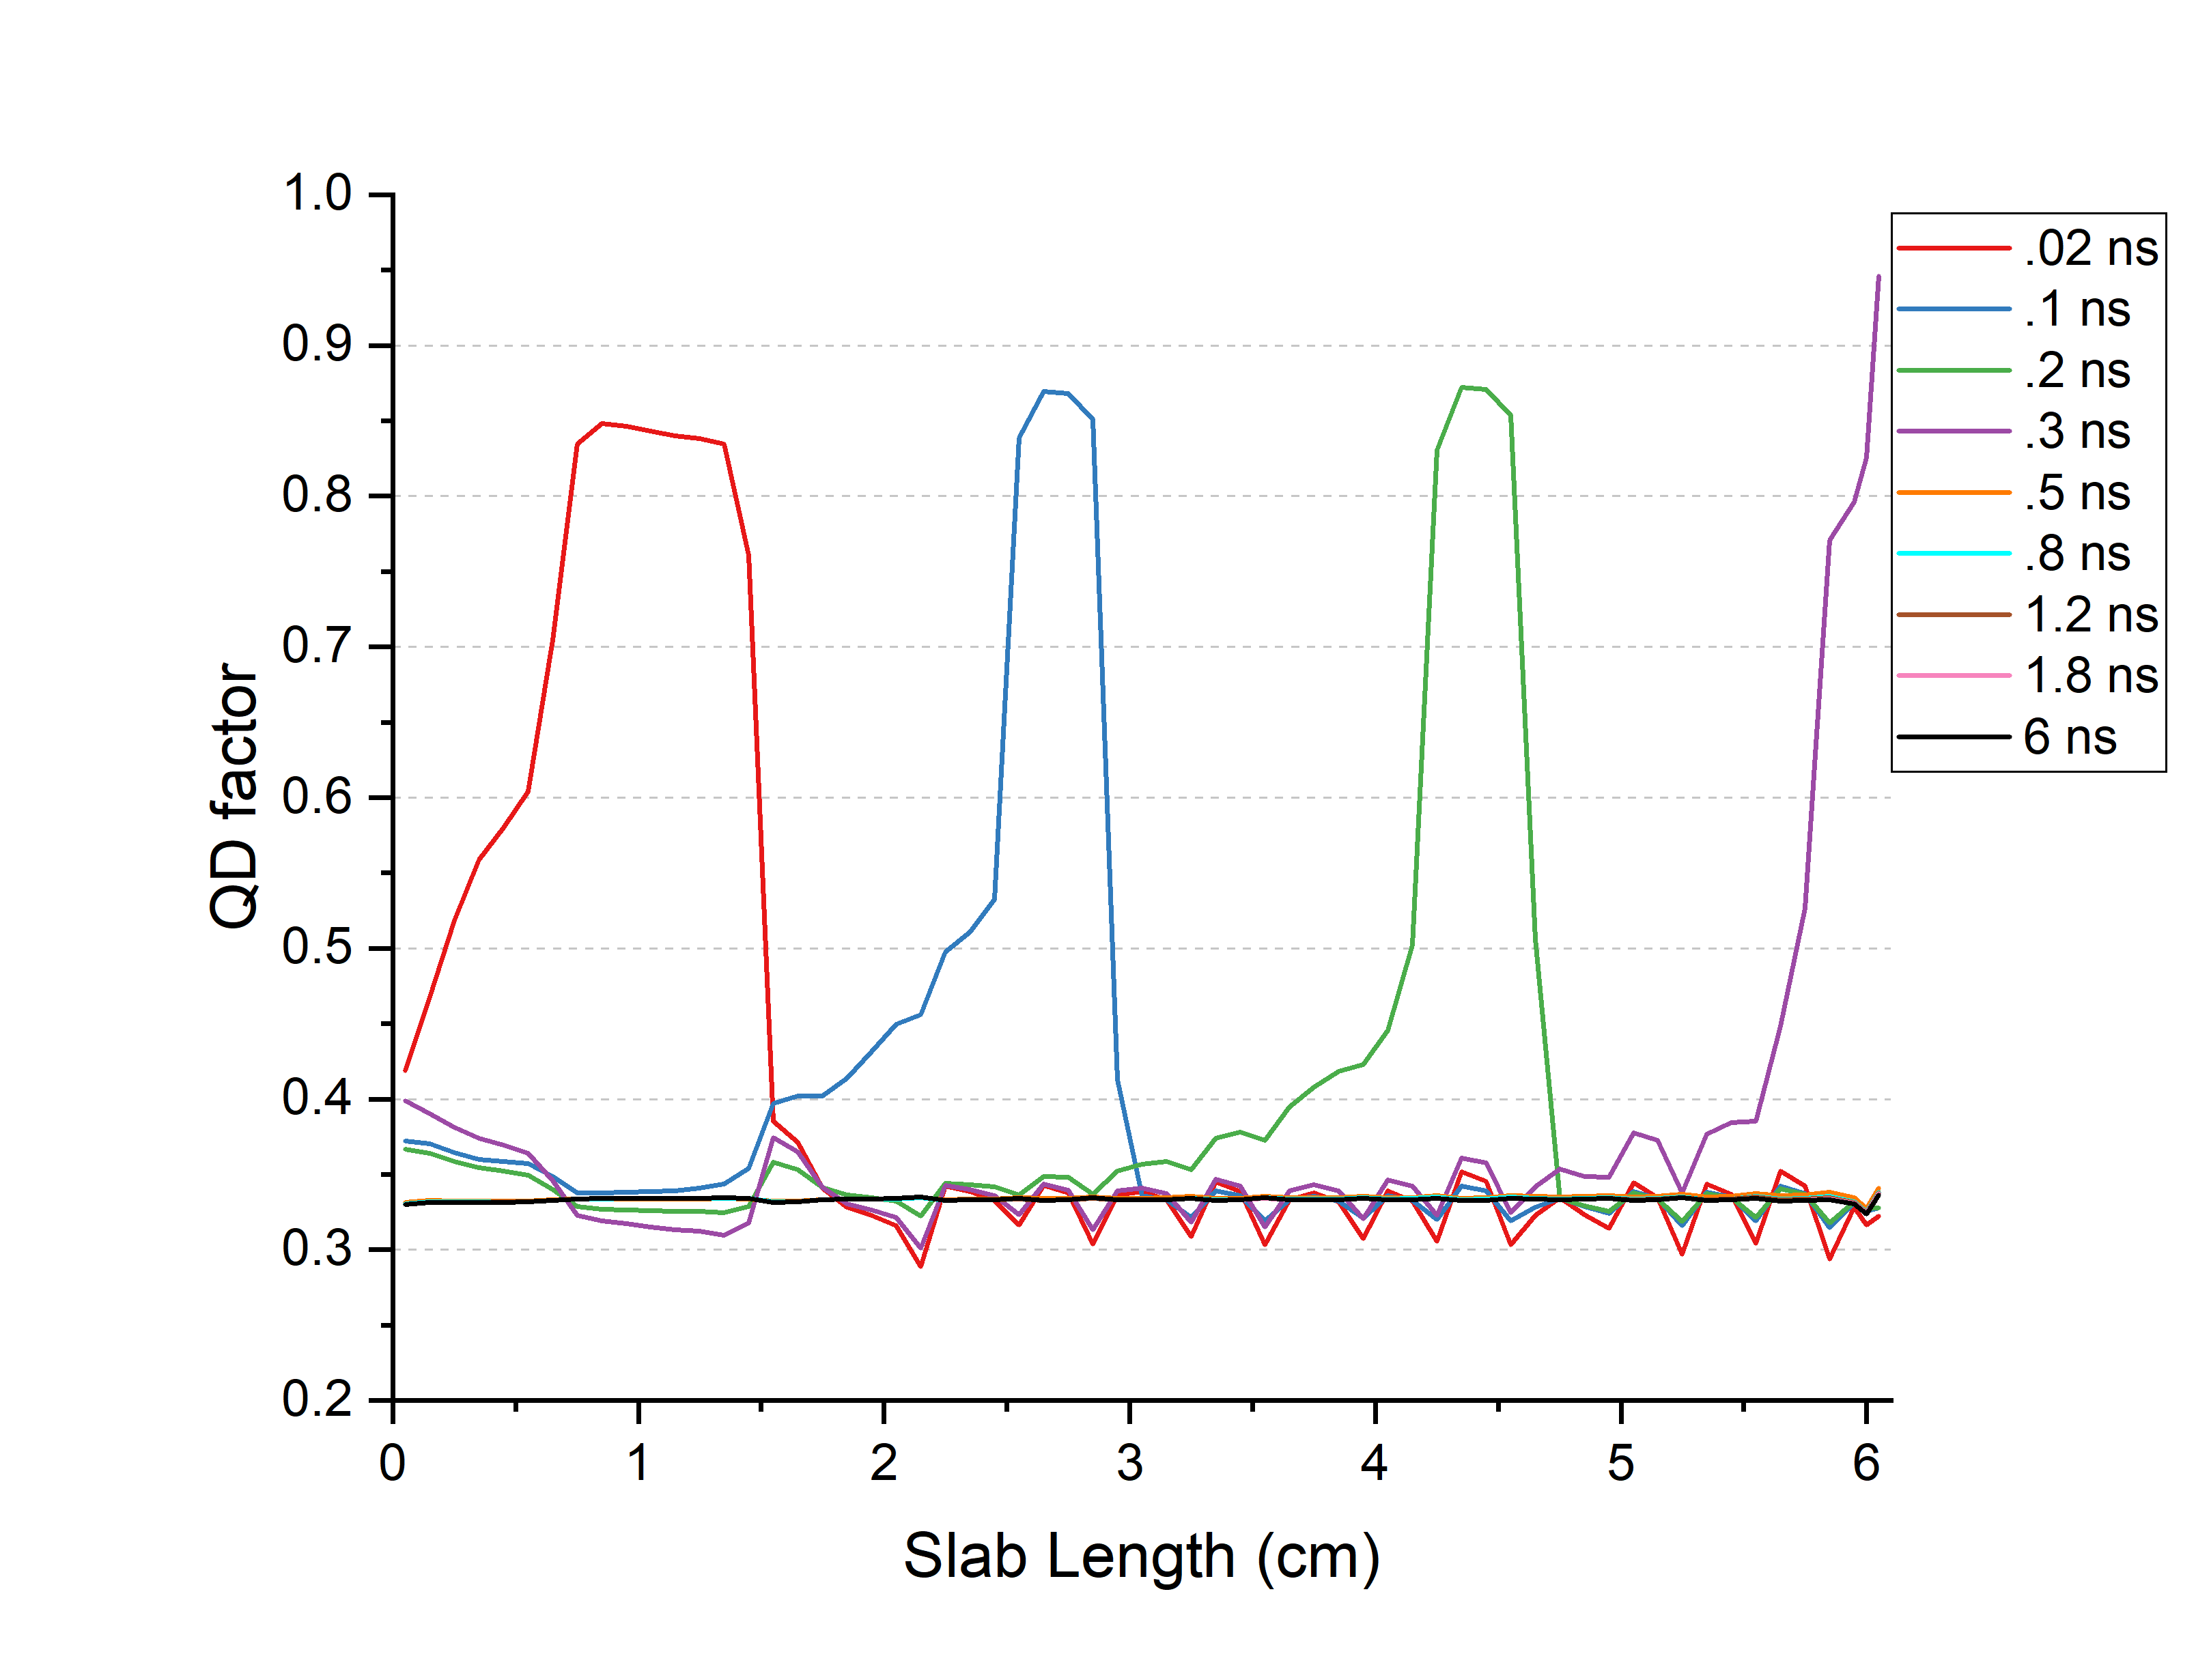
\includegraphics[width=0.5\textwidth]{qdf_g2_cut15.png}}
		\subfloat[r = 20 \label{subfig:qdf_g2_cut20}]{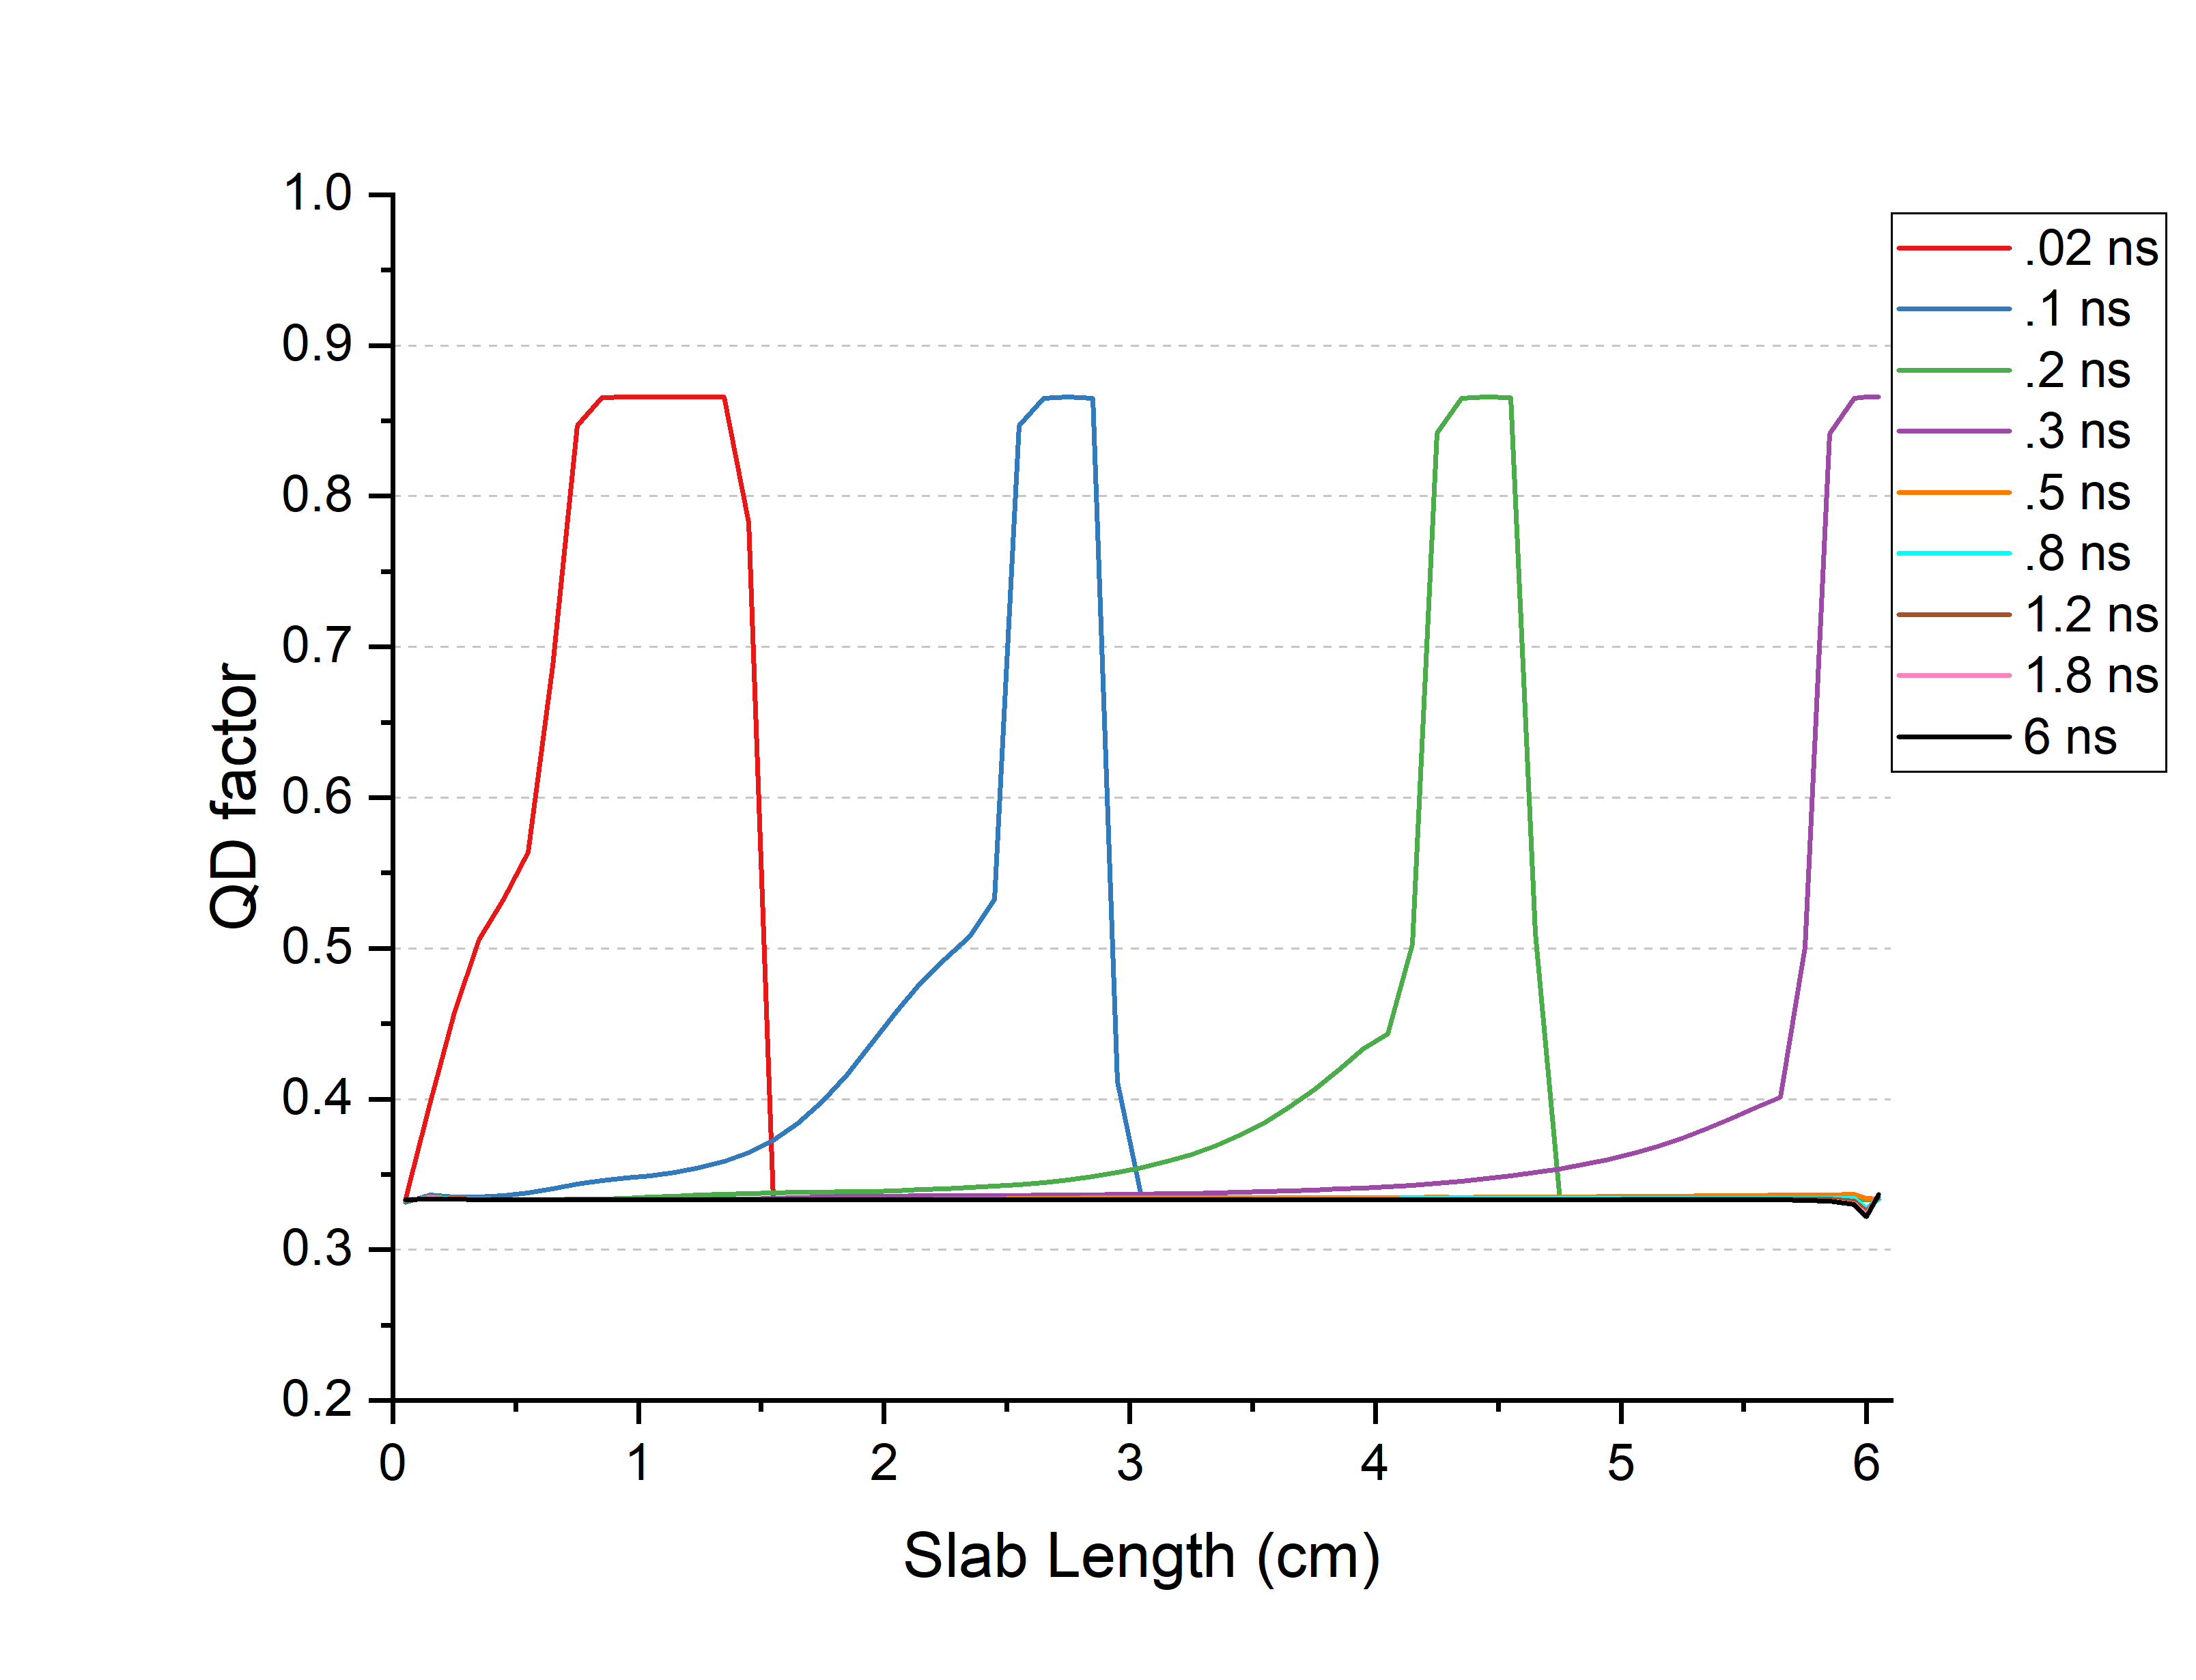
\includegraphics[width=0.5\textwidth]{qdf_g2_cut20.png}}
		\caption{\label{fig:qdf_g2_recomps}
			Low-rank approximation of the group QD factors for $g=2$ for select time steps}
	\end{figure}

	%=================================================================================
	% QDF G3 RECOMP
	\begin{figure}[ht!]
		\centering
		\subfloat[r = 1 \label{subfig:qdf_g3_cut1}]{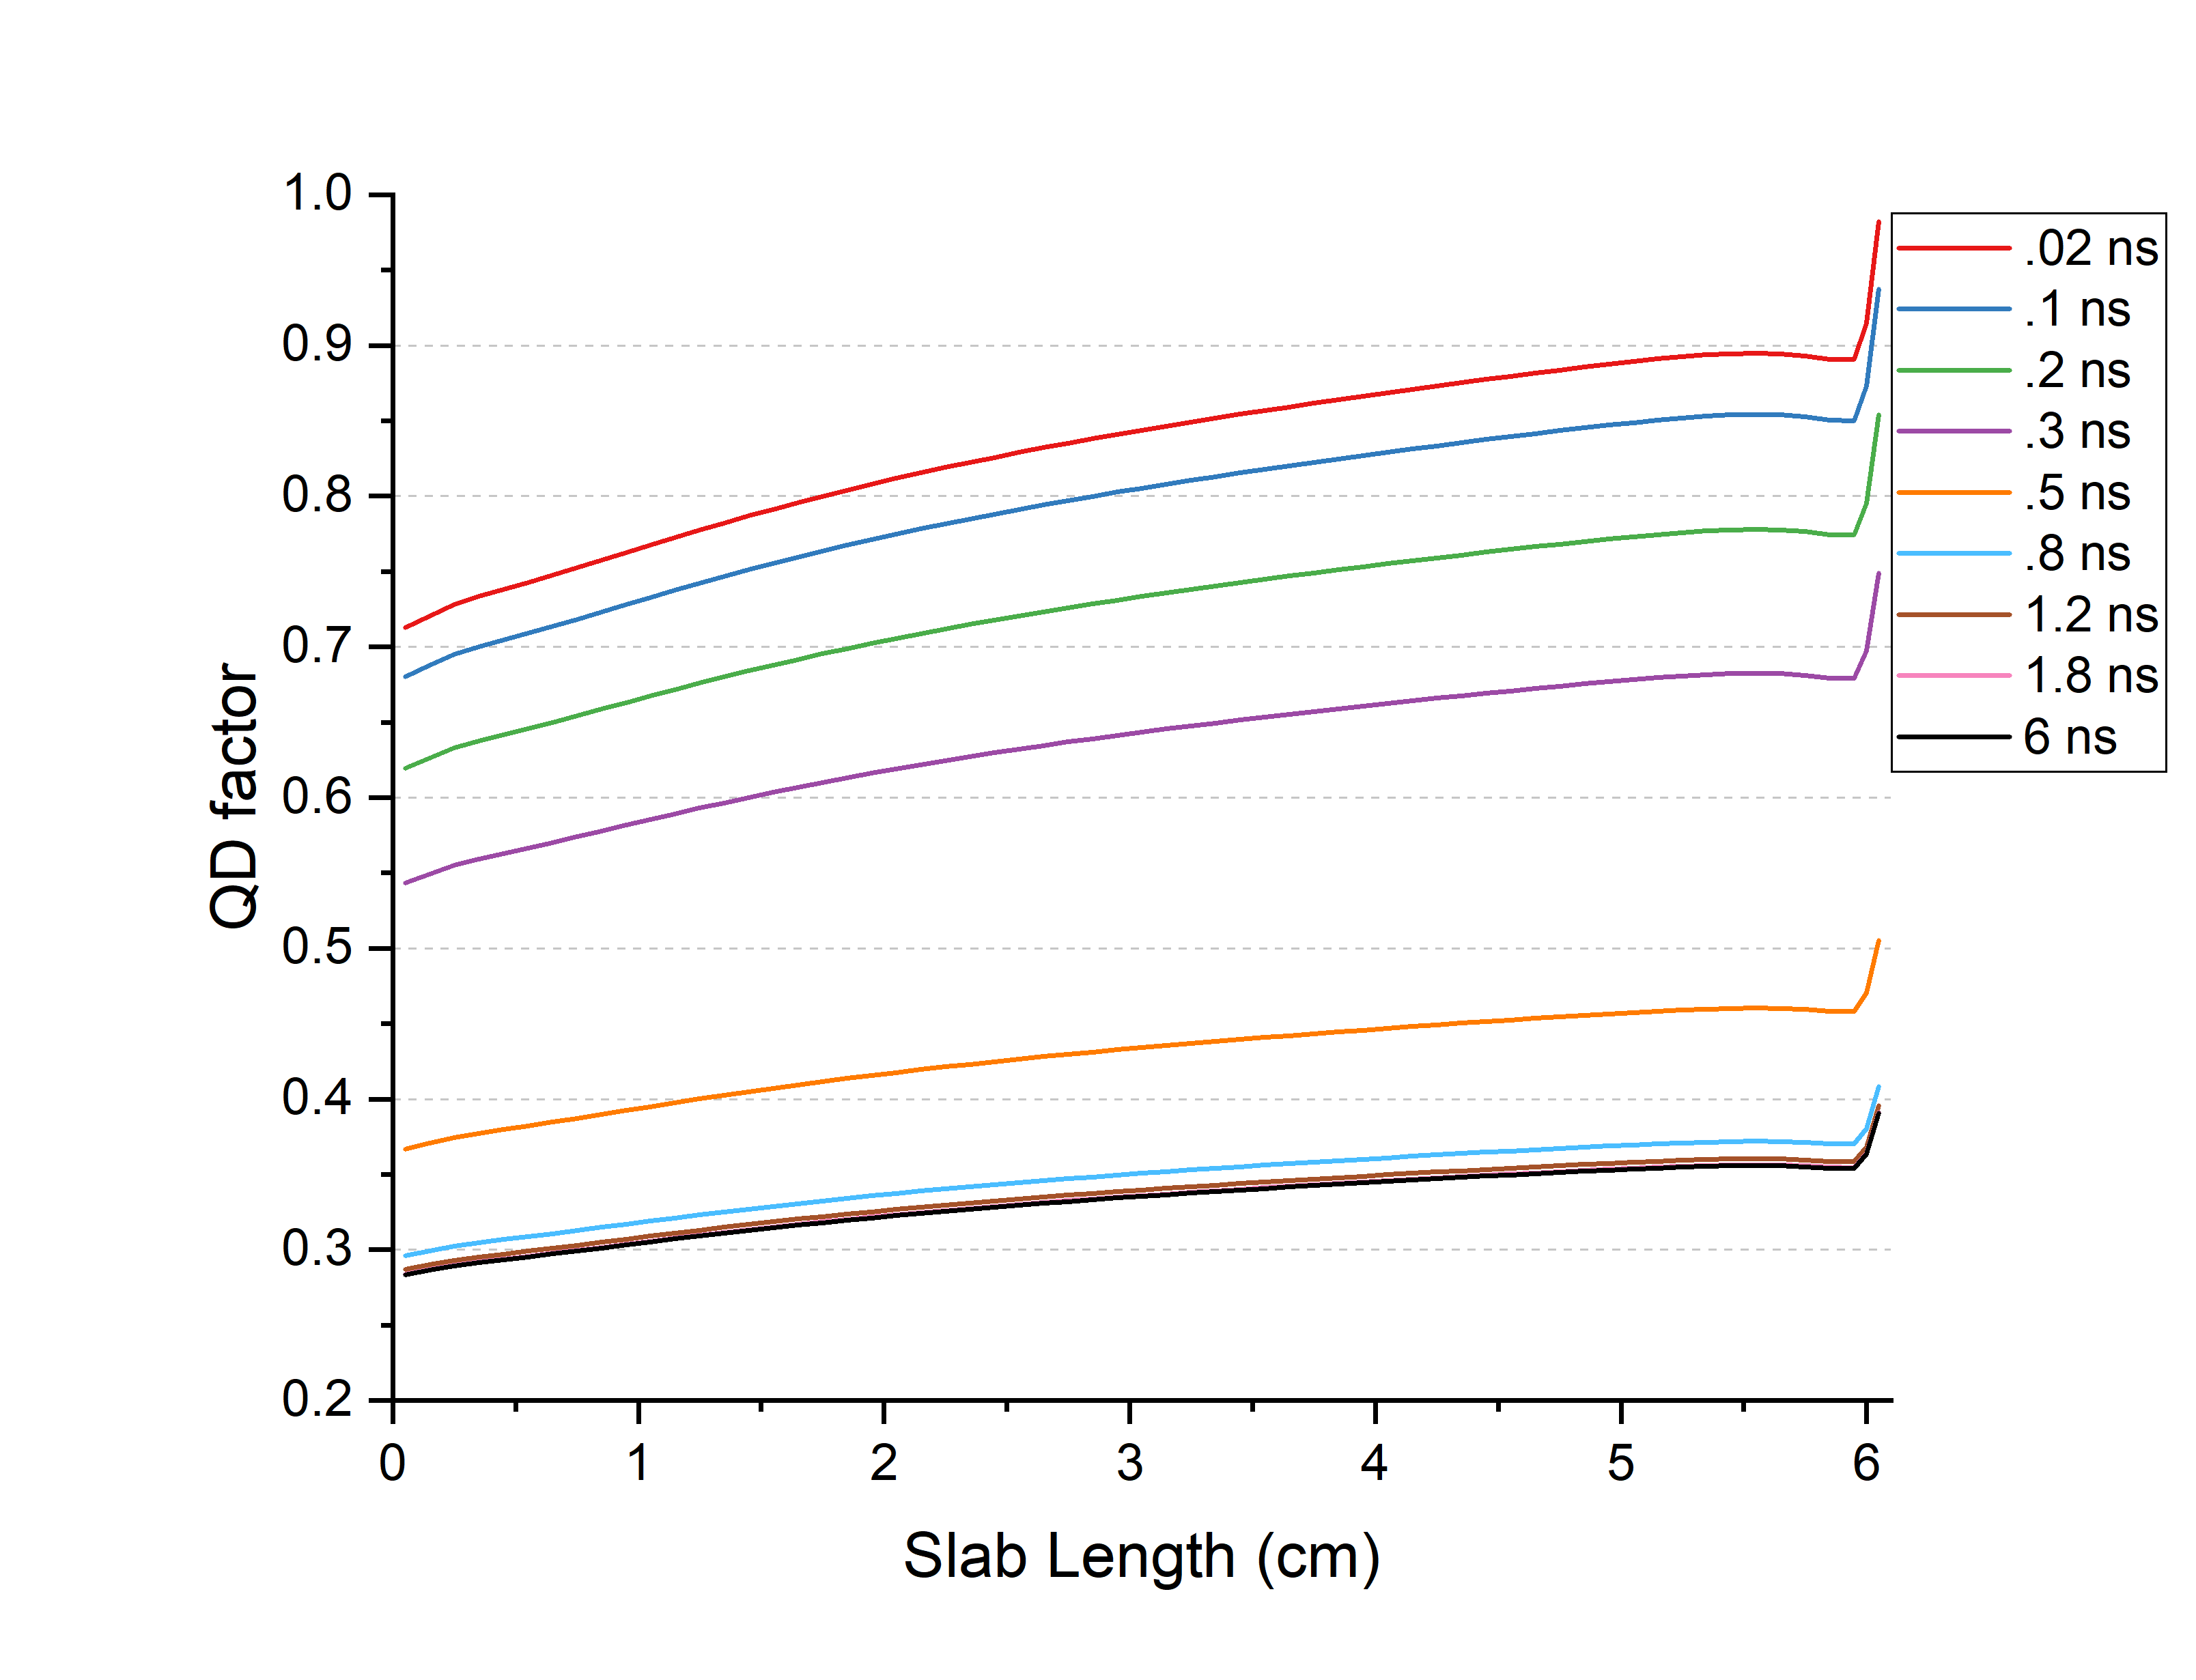
\includegraphics[width=0.5\textwidth]{qdf_g3_cut1.png}}
		\subfloat[r = 2 \label{subfig:qdf_g3_cut2}]{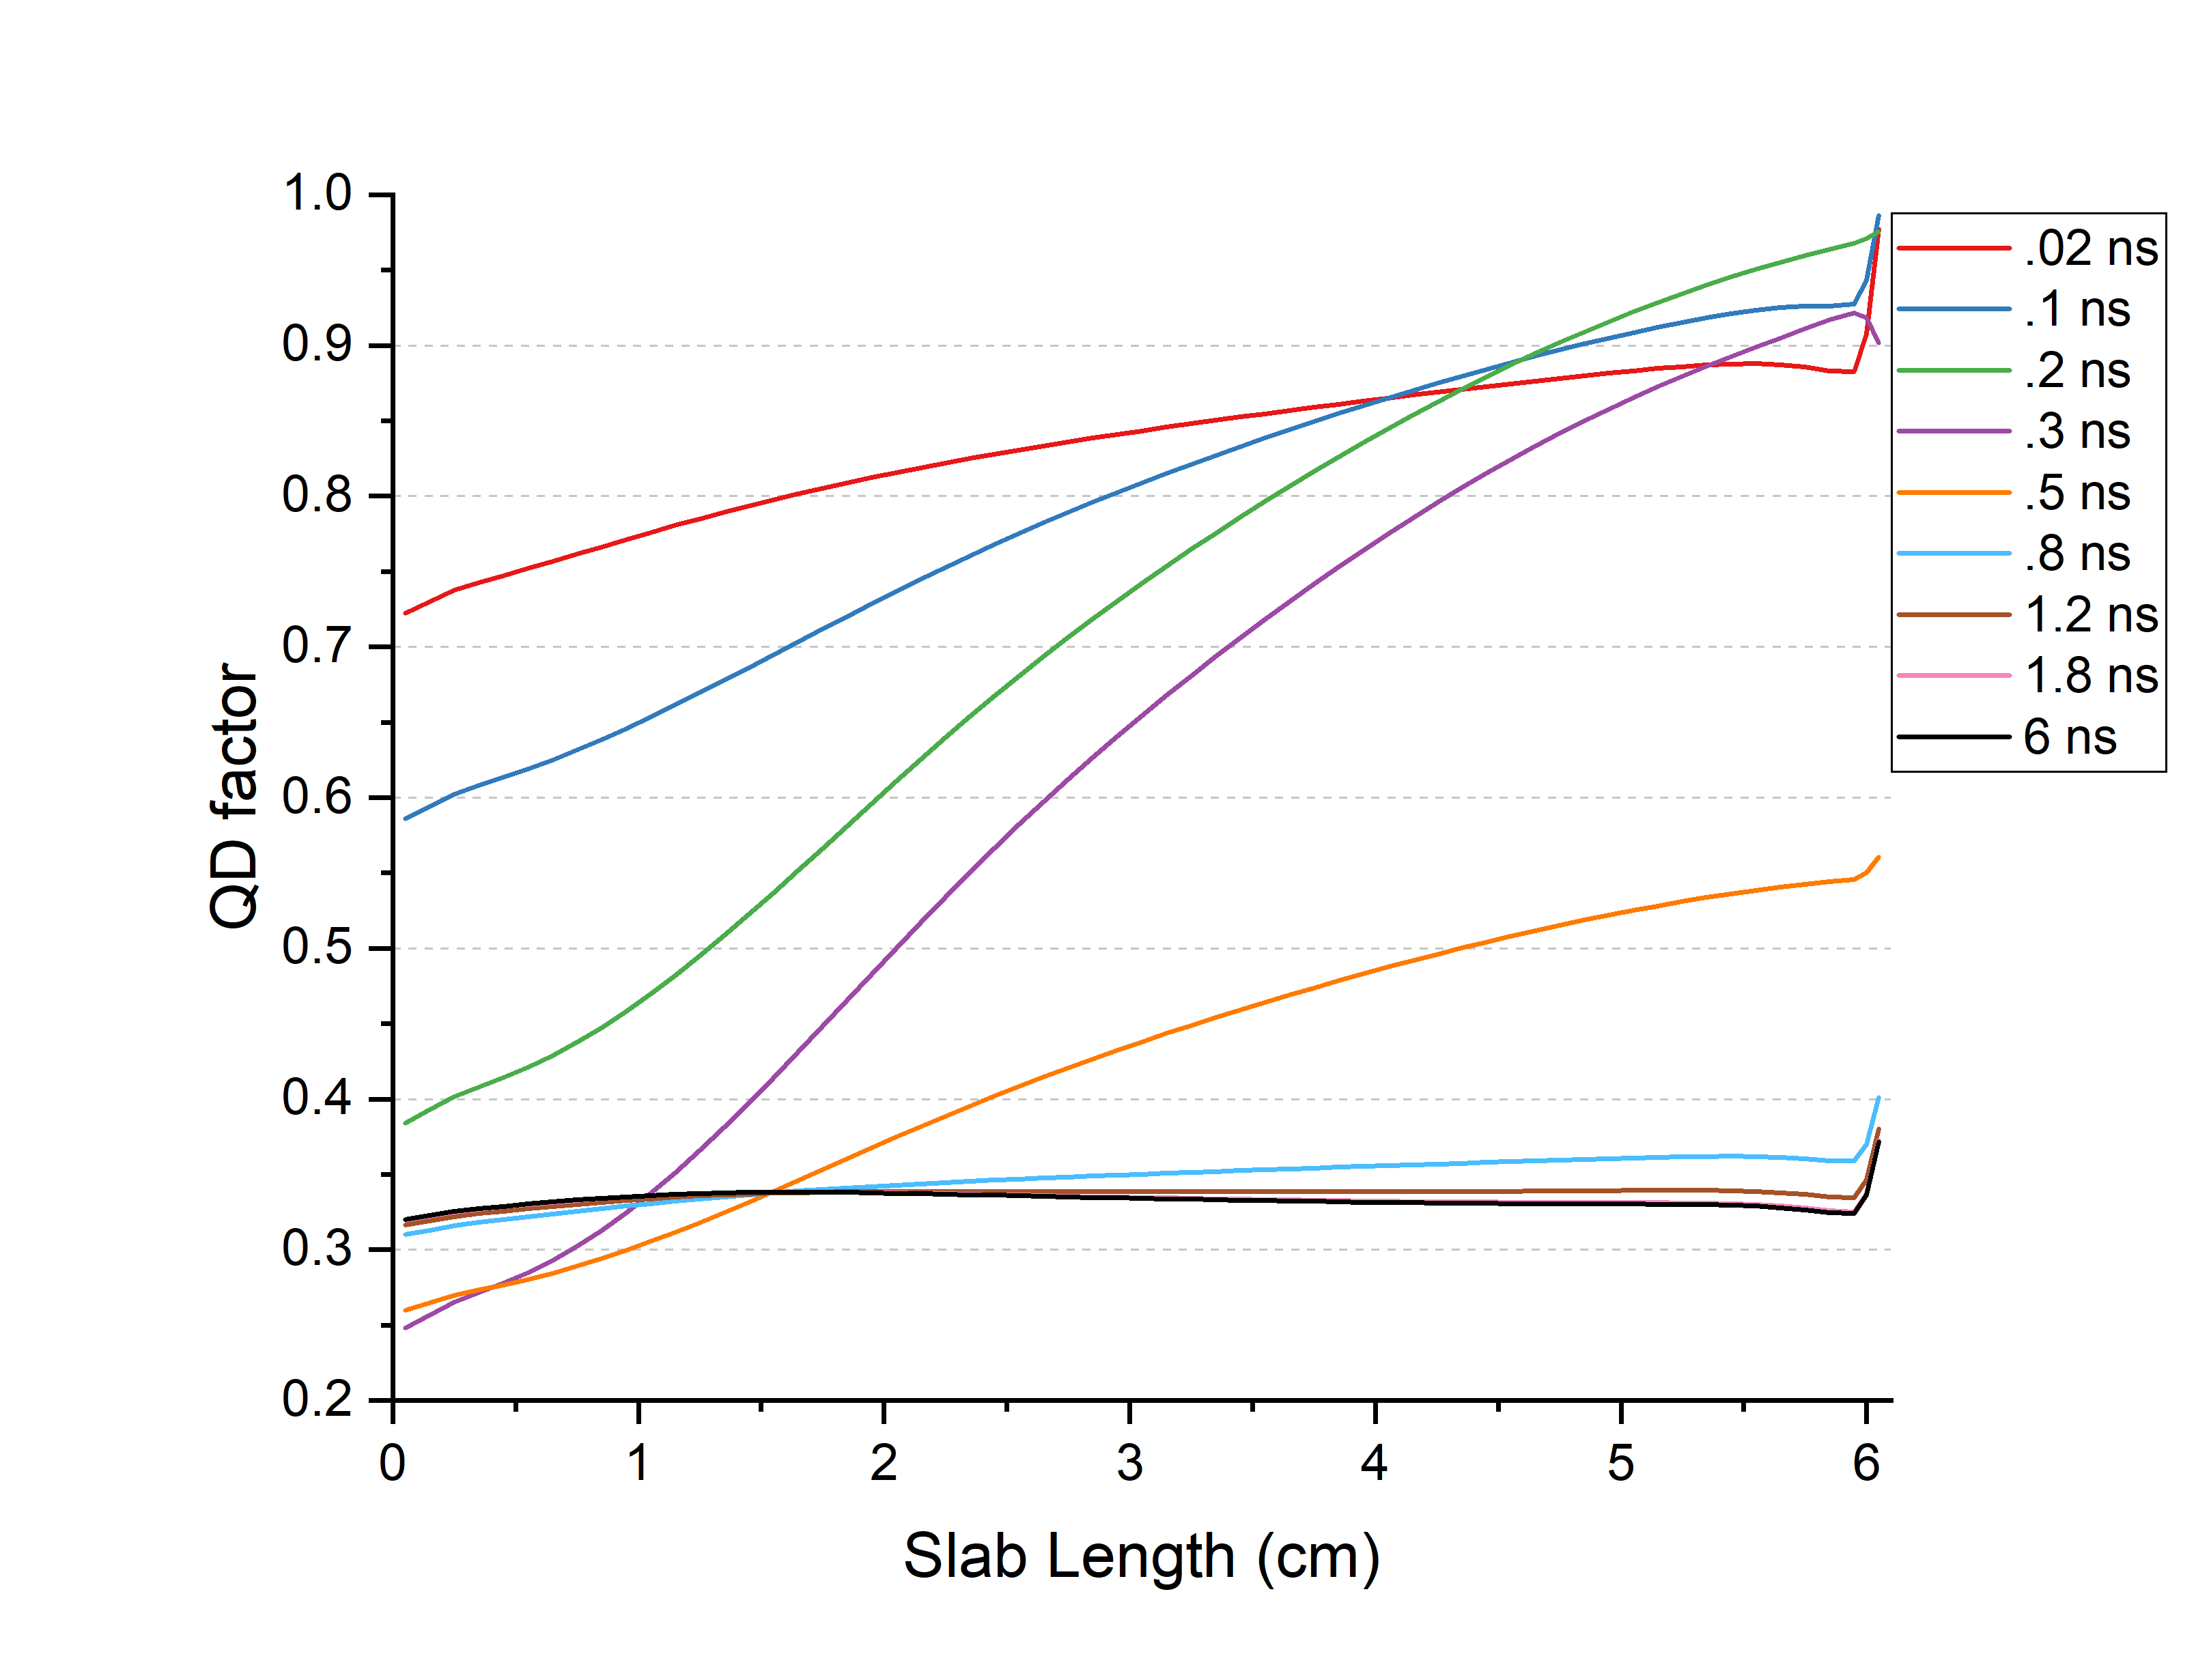
\includegraphics[width=0.5\textwidth]{qdf_g3_cut2.png}}\\
		\subfloat[r = 5 \label{subfig:qdf_g3_cut5}]{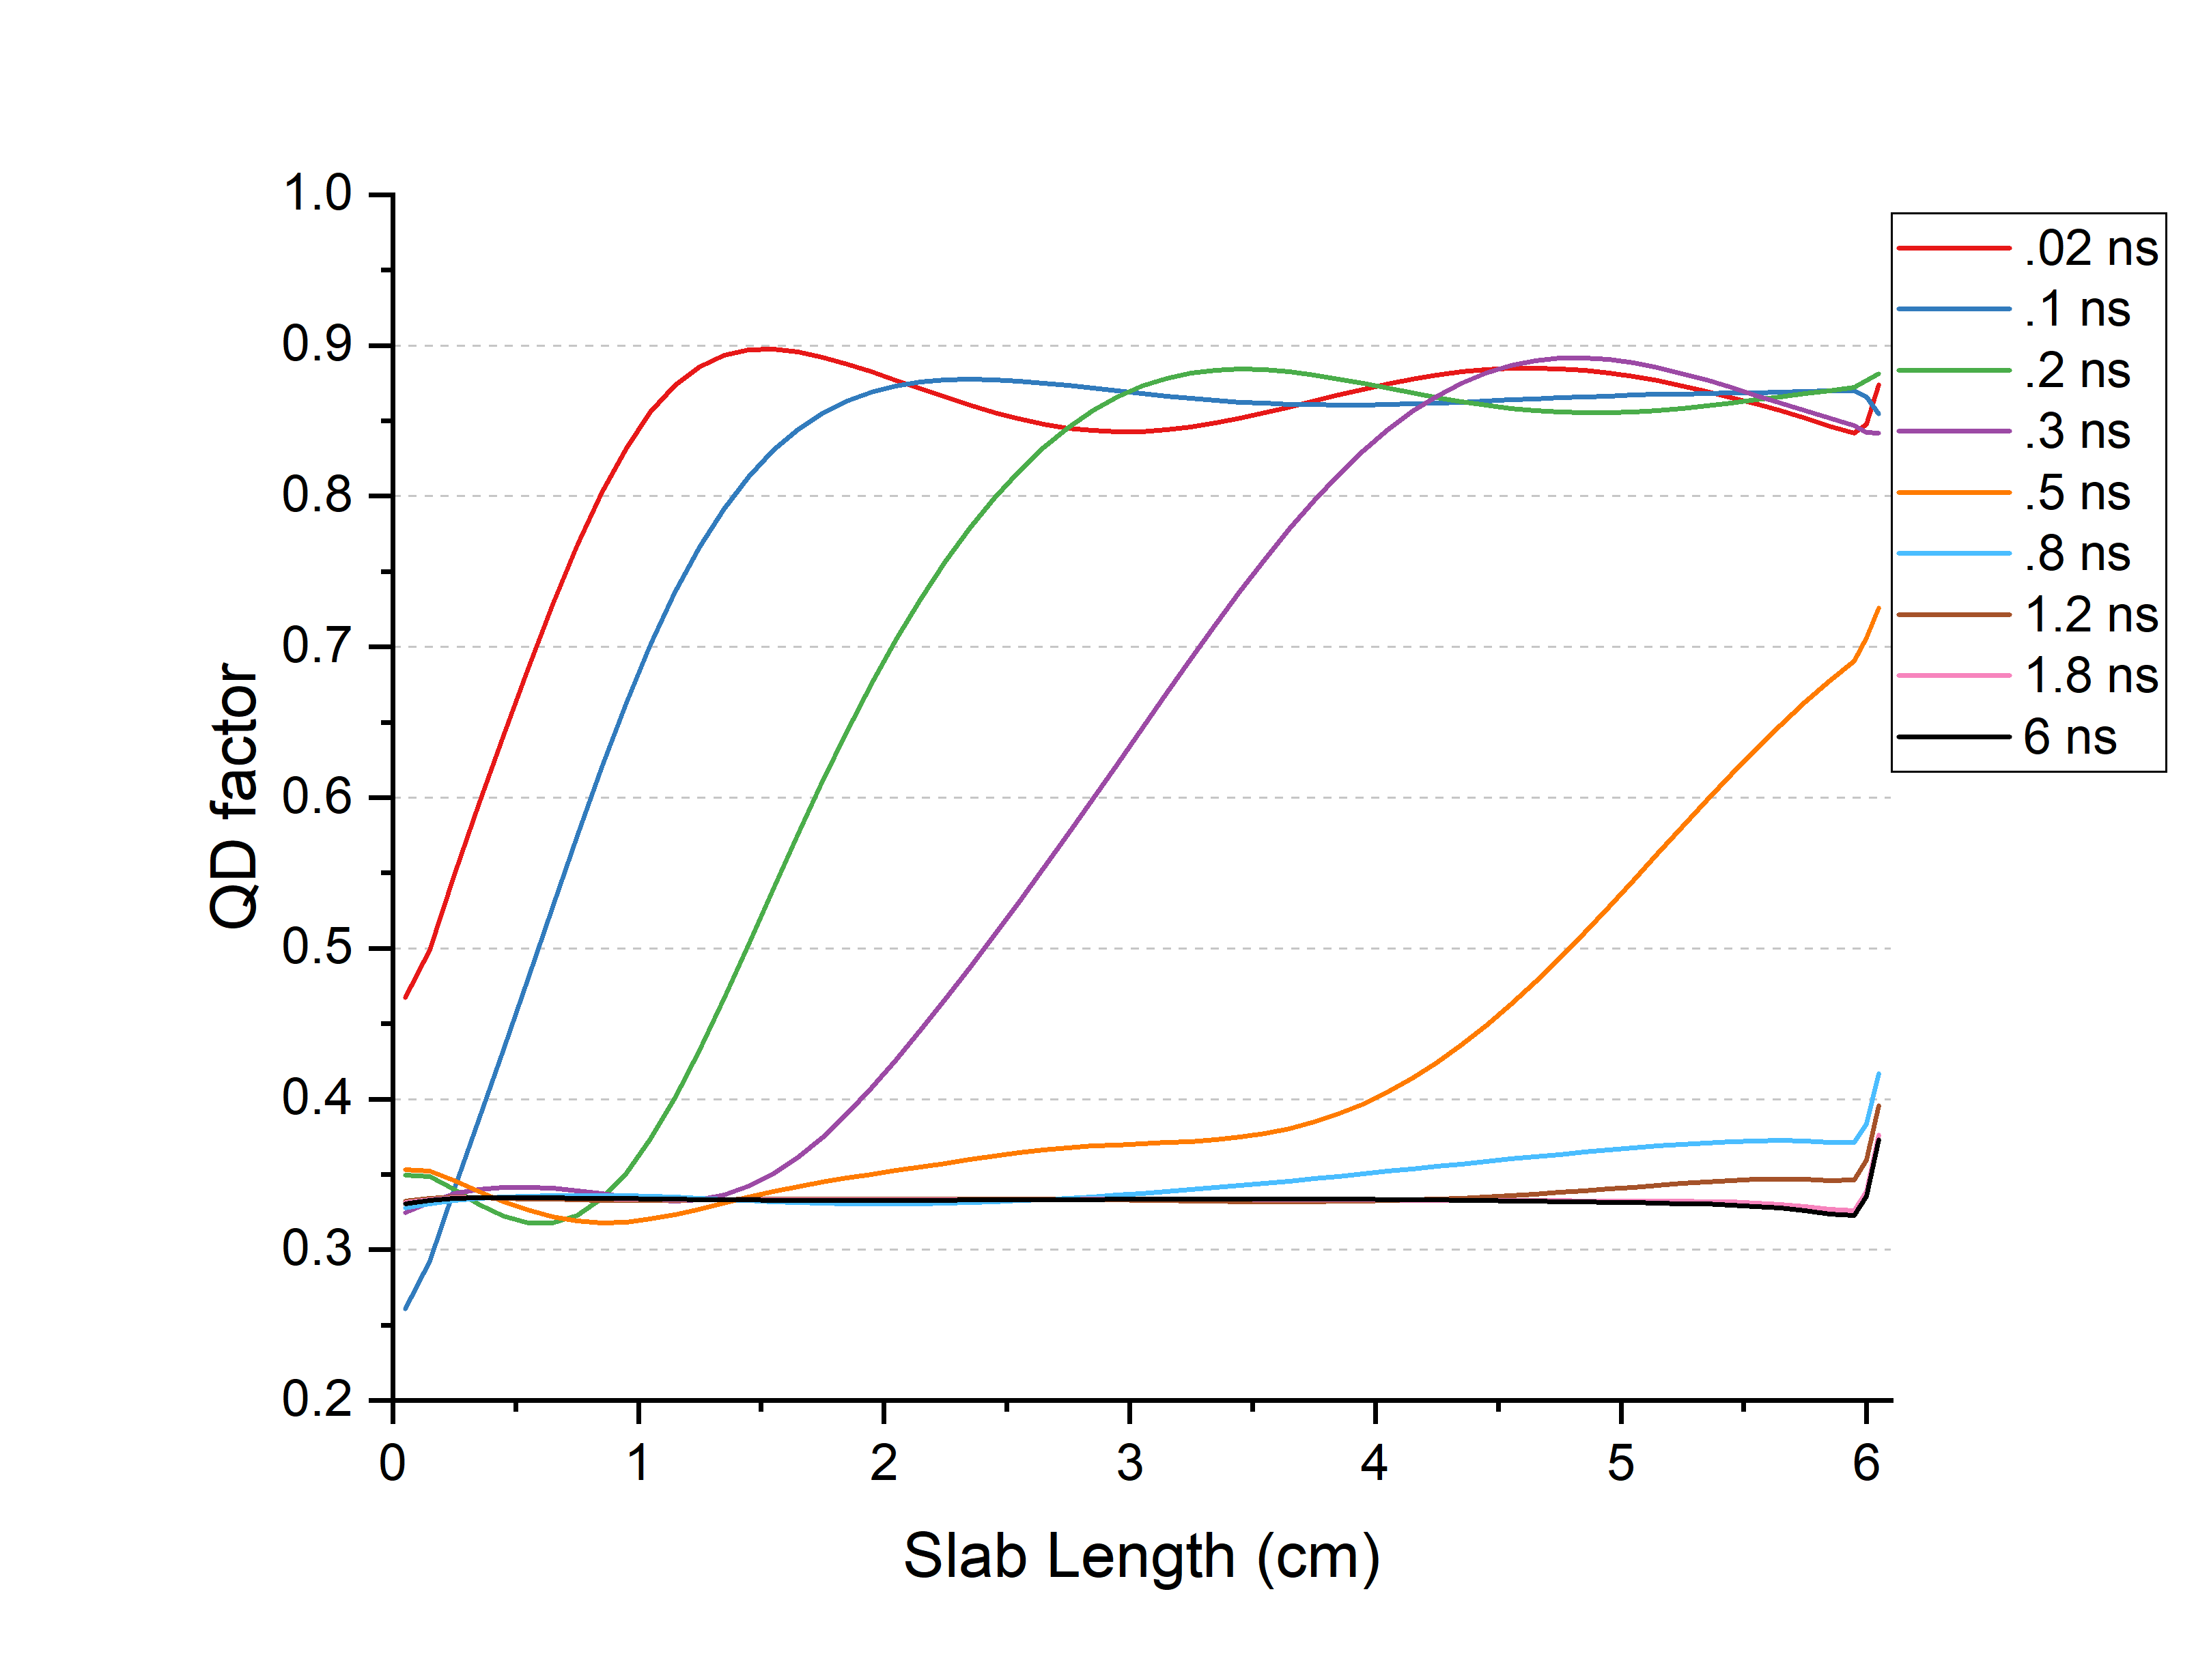
\includegraphics[width=0.5\textwidth]{qdf_g3_cut5.png}}
		\subfloat[r = 10 \label{subfig:qdf_g3_cut10}]{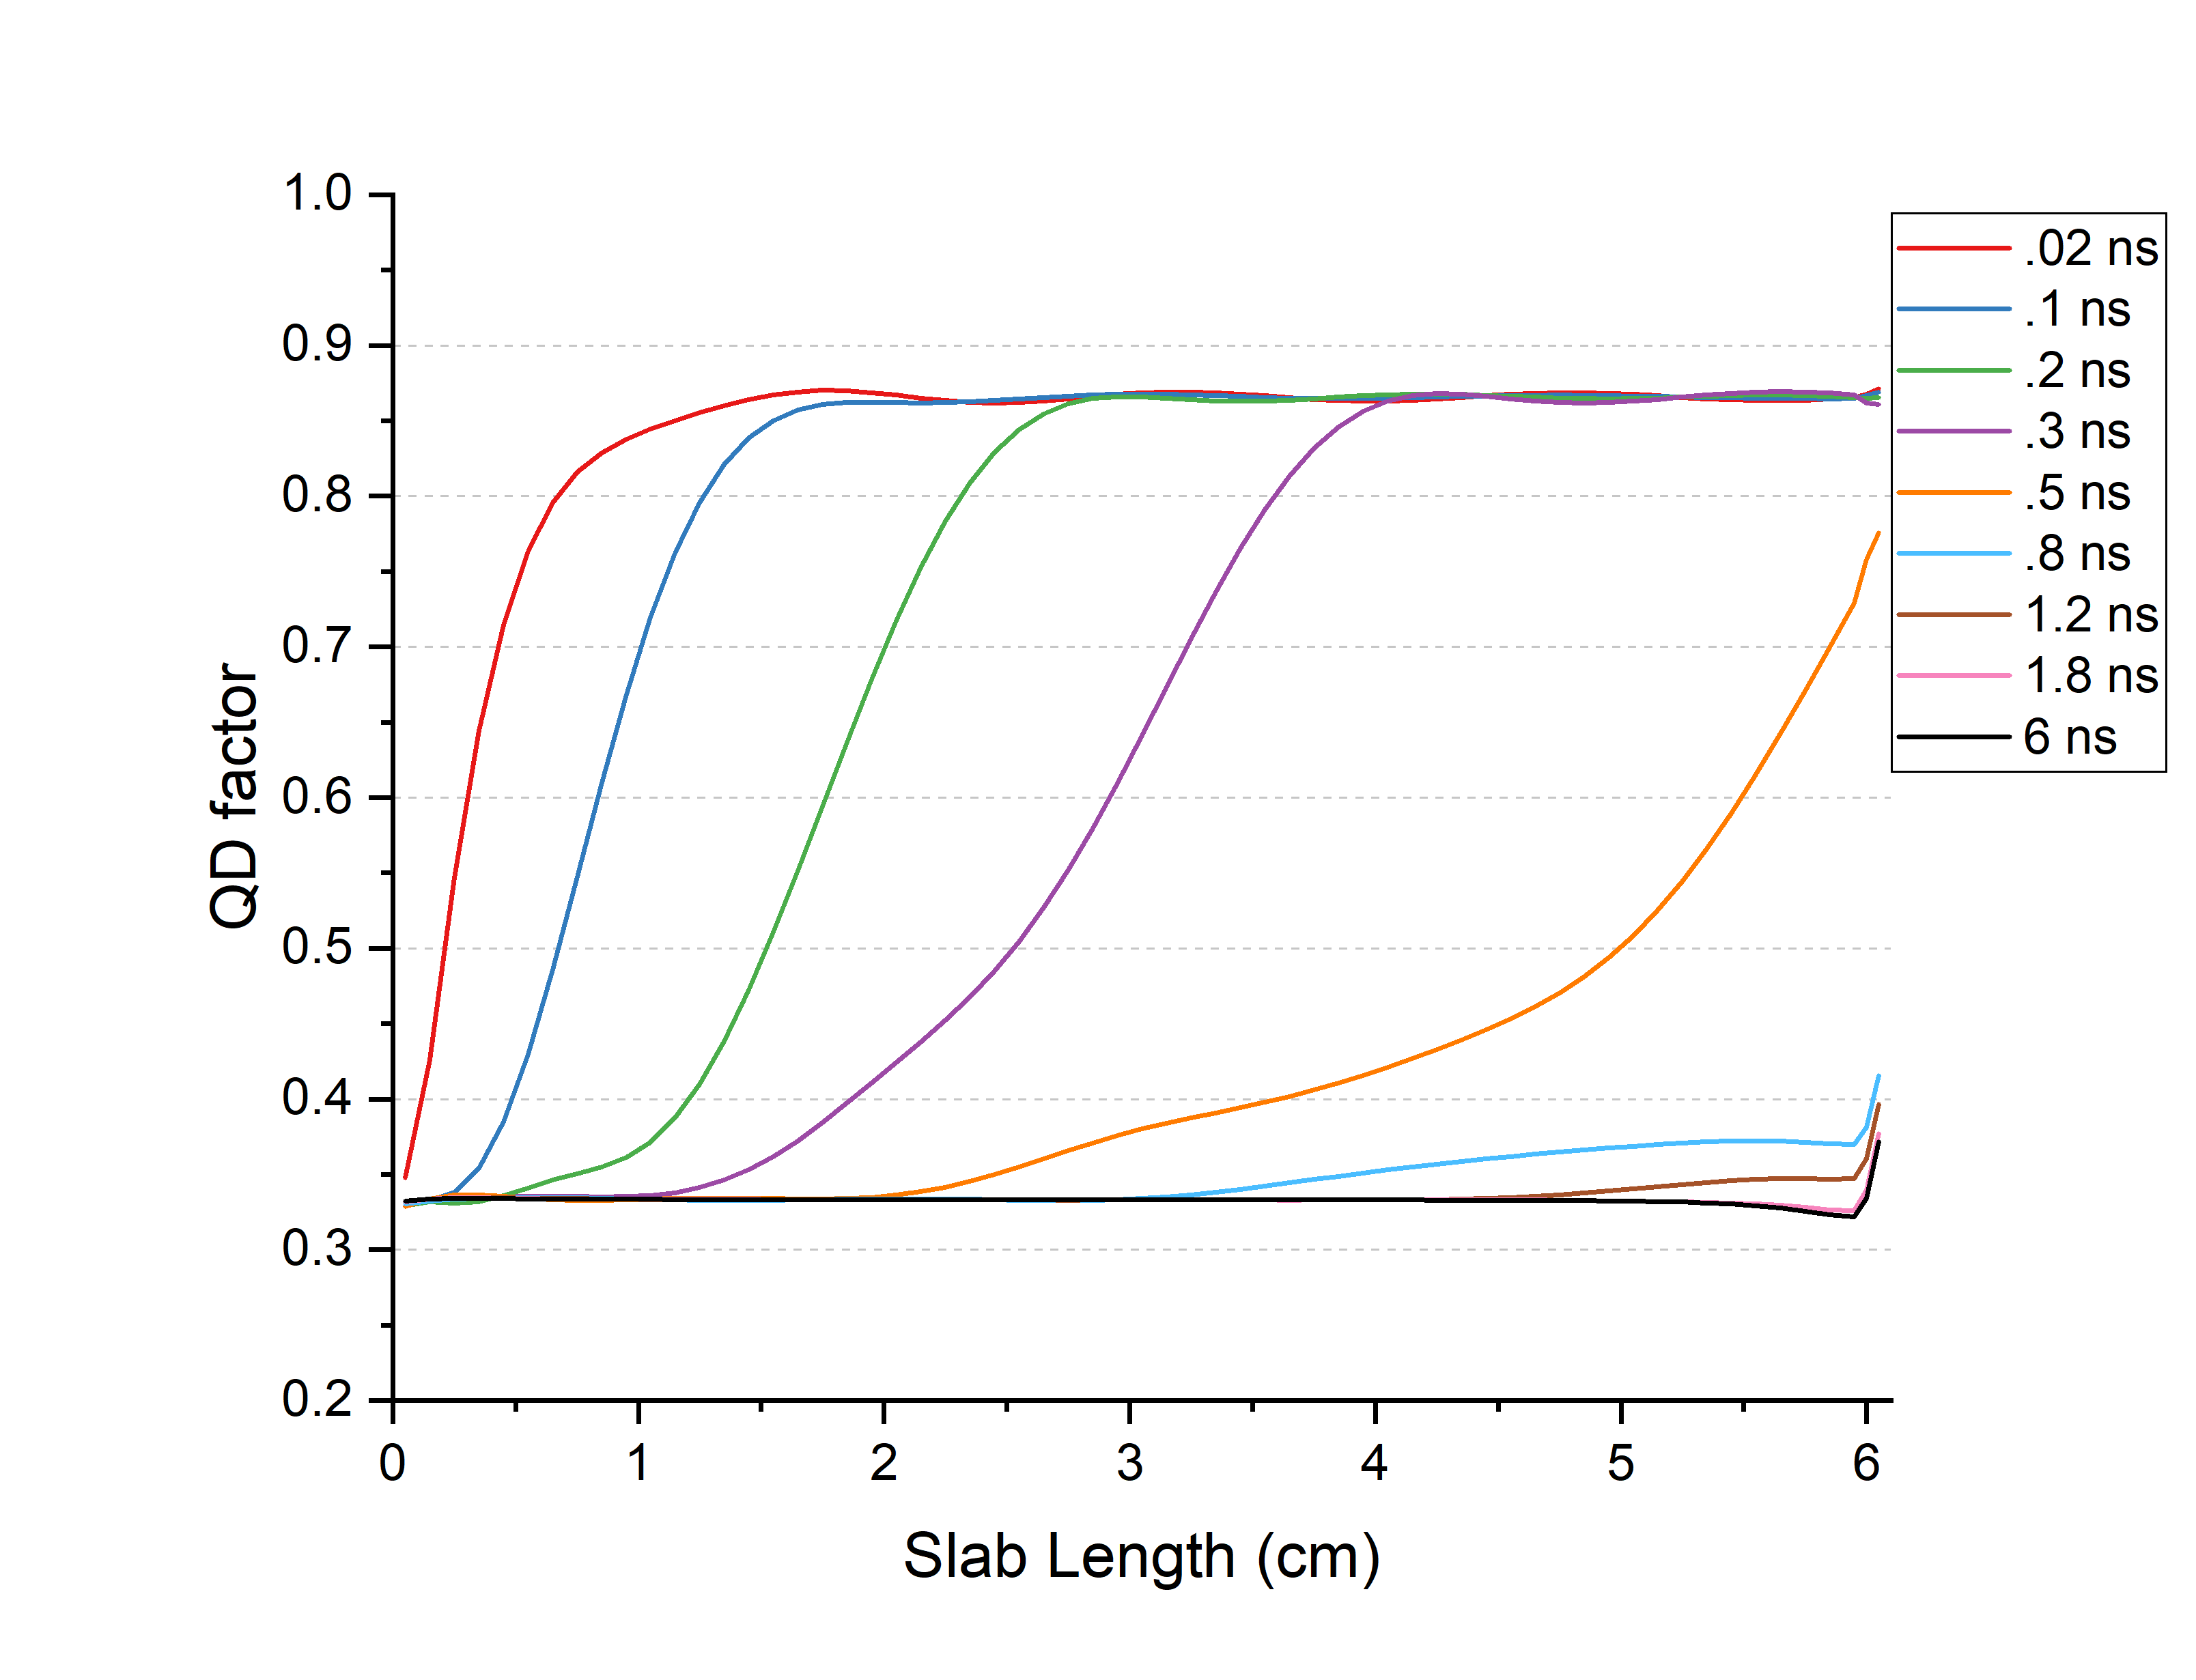
\includegraphics[width=0.5\textwidth]{qdf_g3_cut10.png}}\\
		\subfloat[r = 15 \label{subfig:qdf_g3_cut15}]{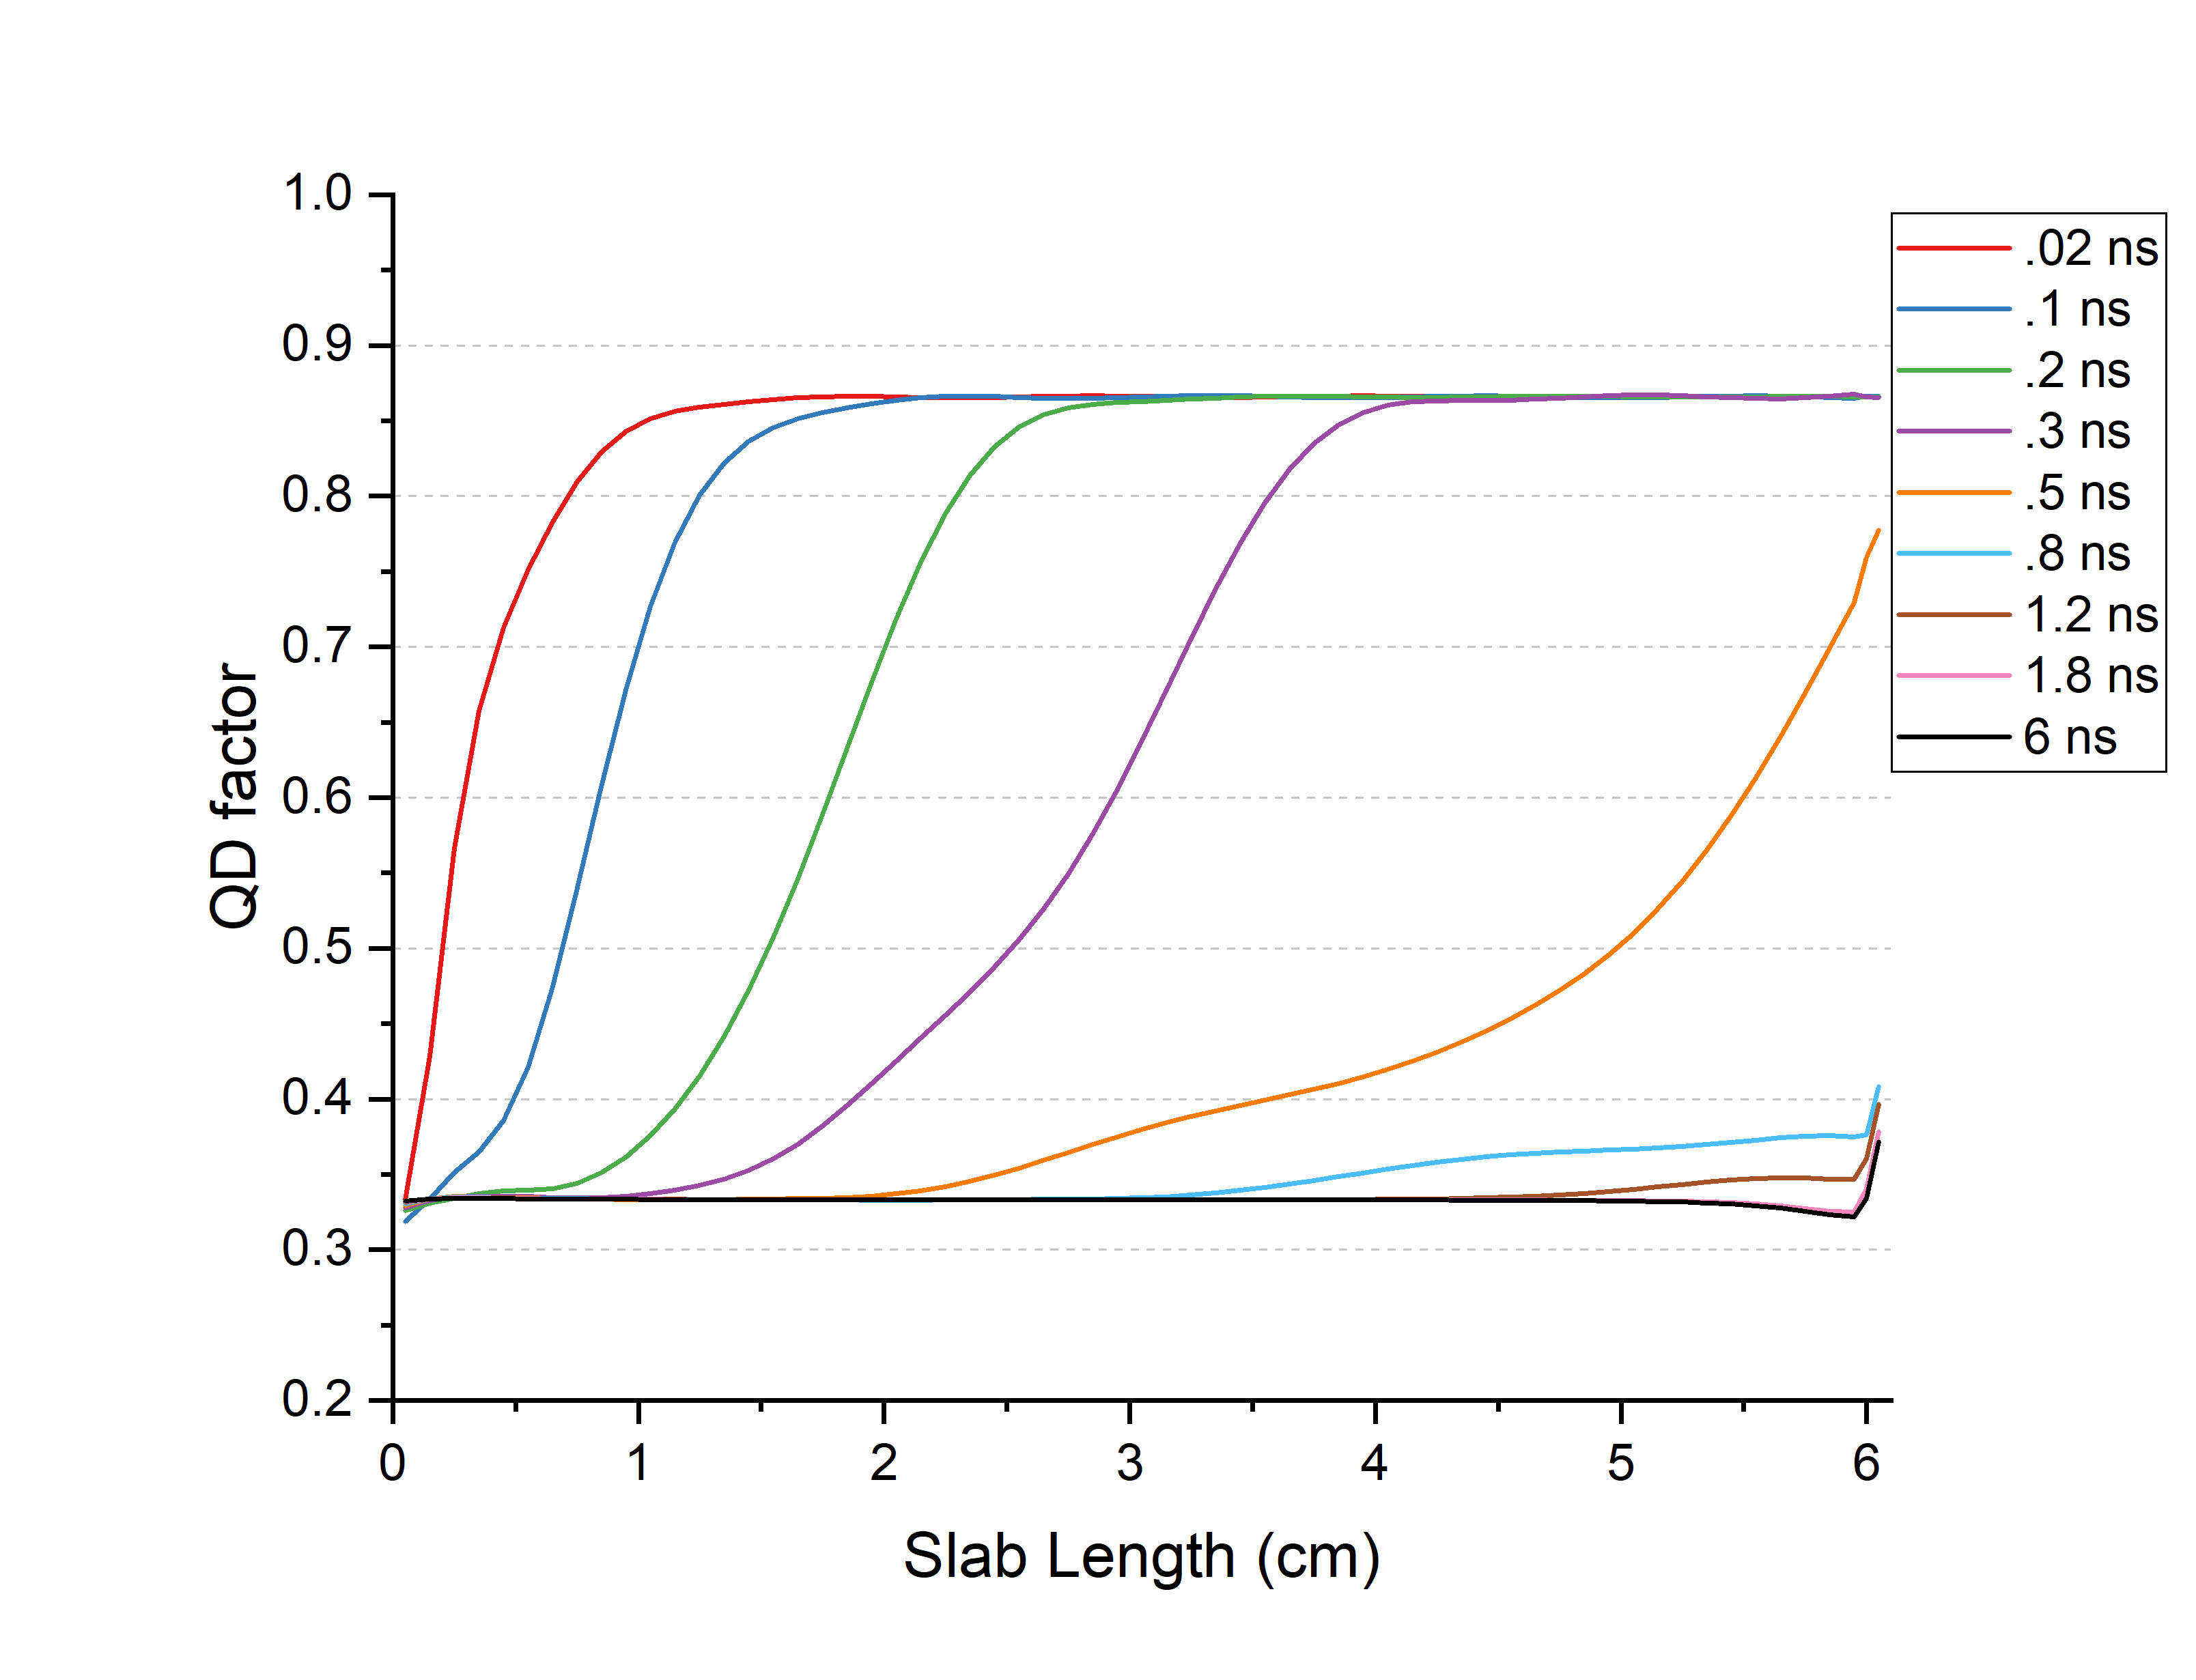
\includegraphics[width=0.5\textwidth]{qdf_g3_cut15.png}}
		\subfloat[r = 20 \label{subfig:qdf_g3_cut20}]{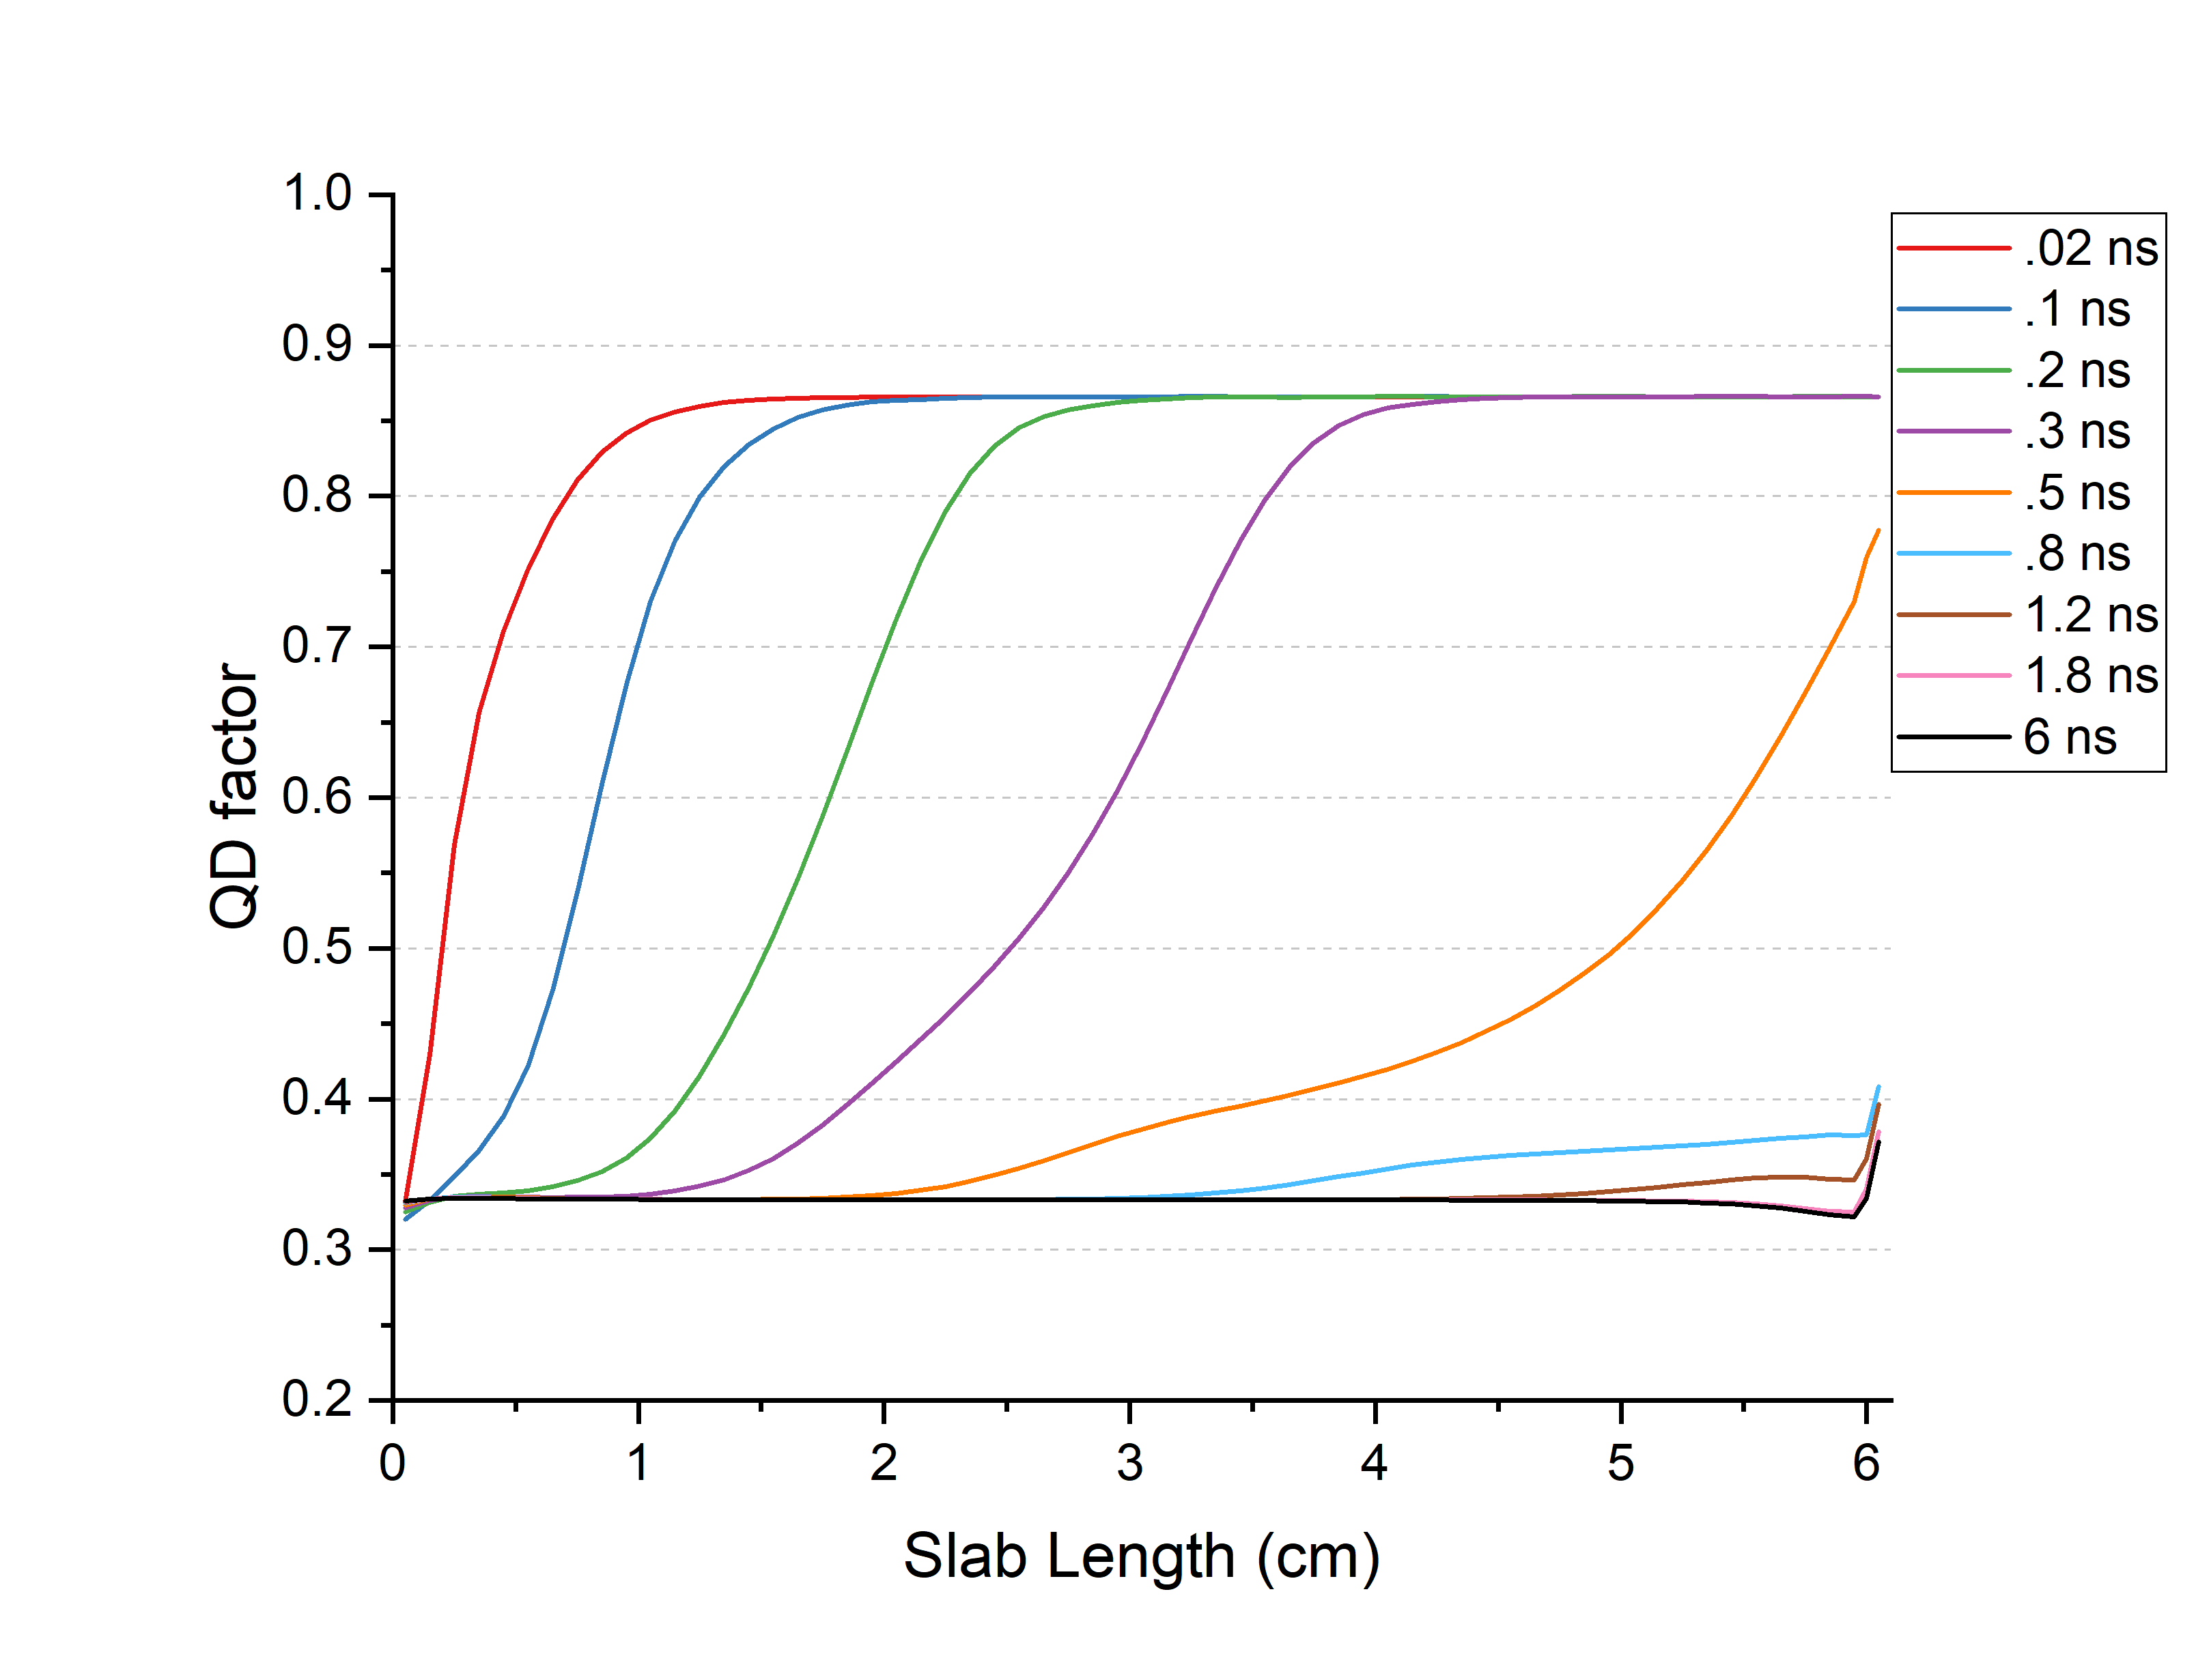
\includegraphics[width=0.5\textwidth]{qdf_g3_cut20.png}}
		\caption{\label{fig:qdf_g3_recomps}
			Low-rank approximation of the group QD factors for $g=3$ for select time steps}
	\end{figure}

	%=================================================================================
	% QDF G8 RECOMP
	\begin{figure}[ht!]
		\centering
		\subfloat[r = 1 \label{subfig:qdf_g8_cut1}]{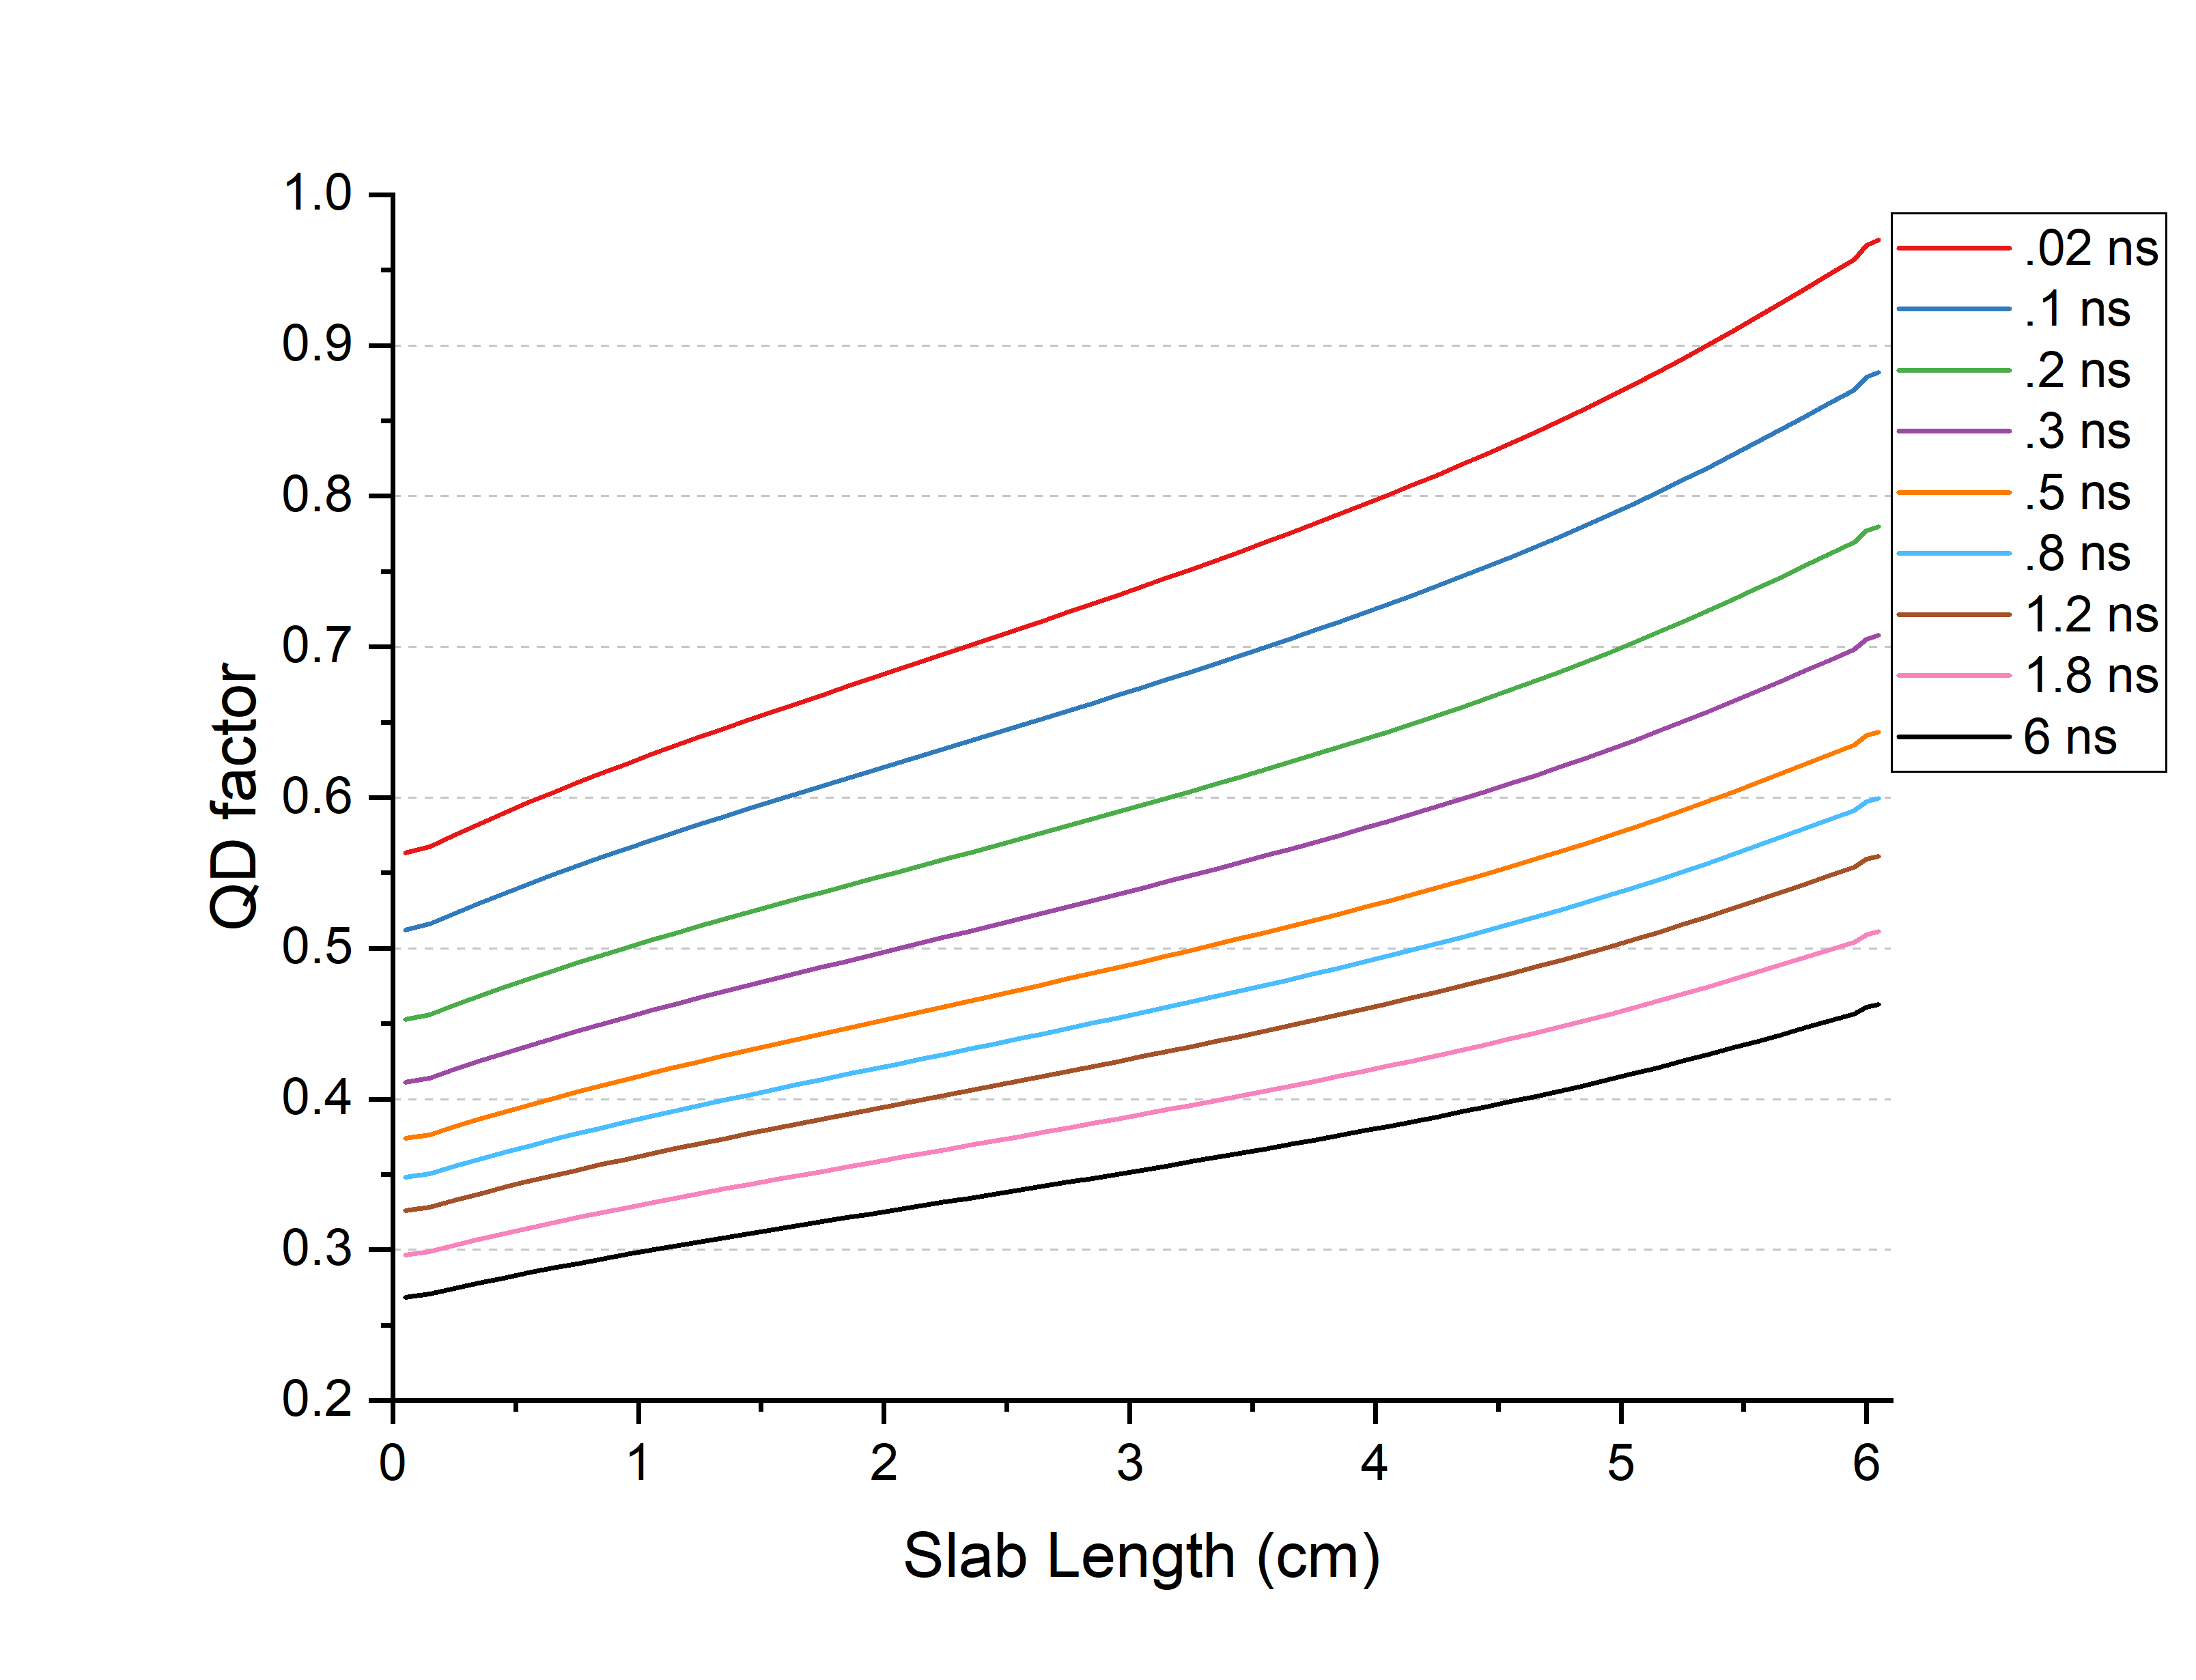
\includegraphics[width=0.5\textwidth]{qdf_g8_cut1.png}}
		\subfloat[r = 2 \label{subfig:qdf_g8_cut2}]{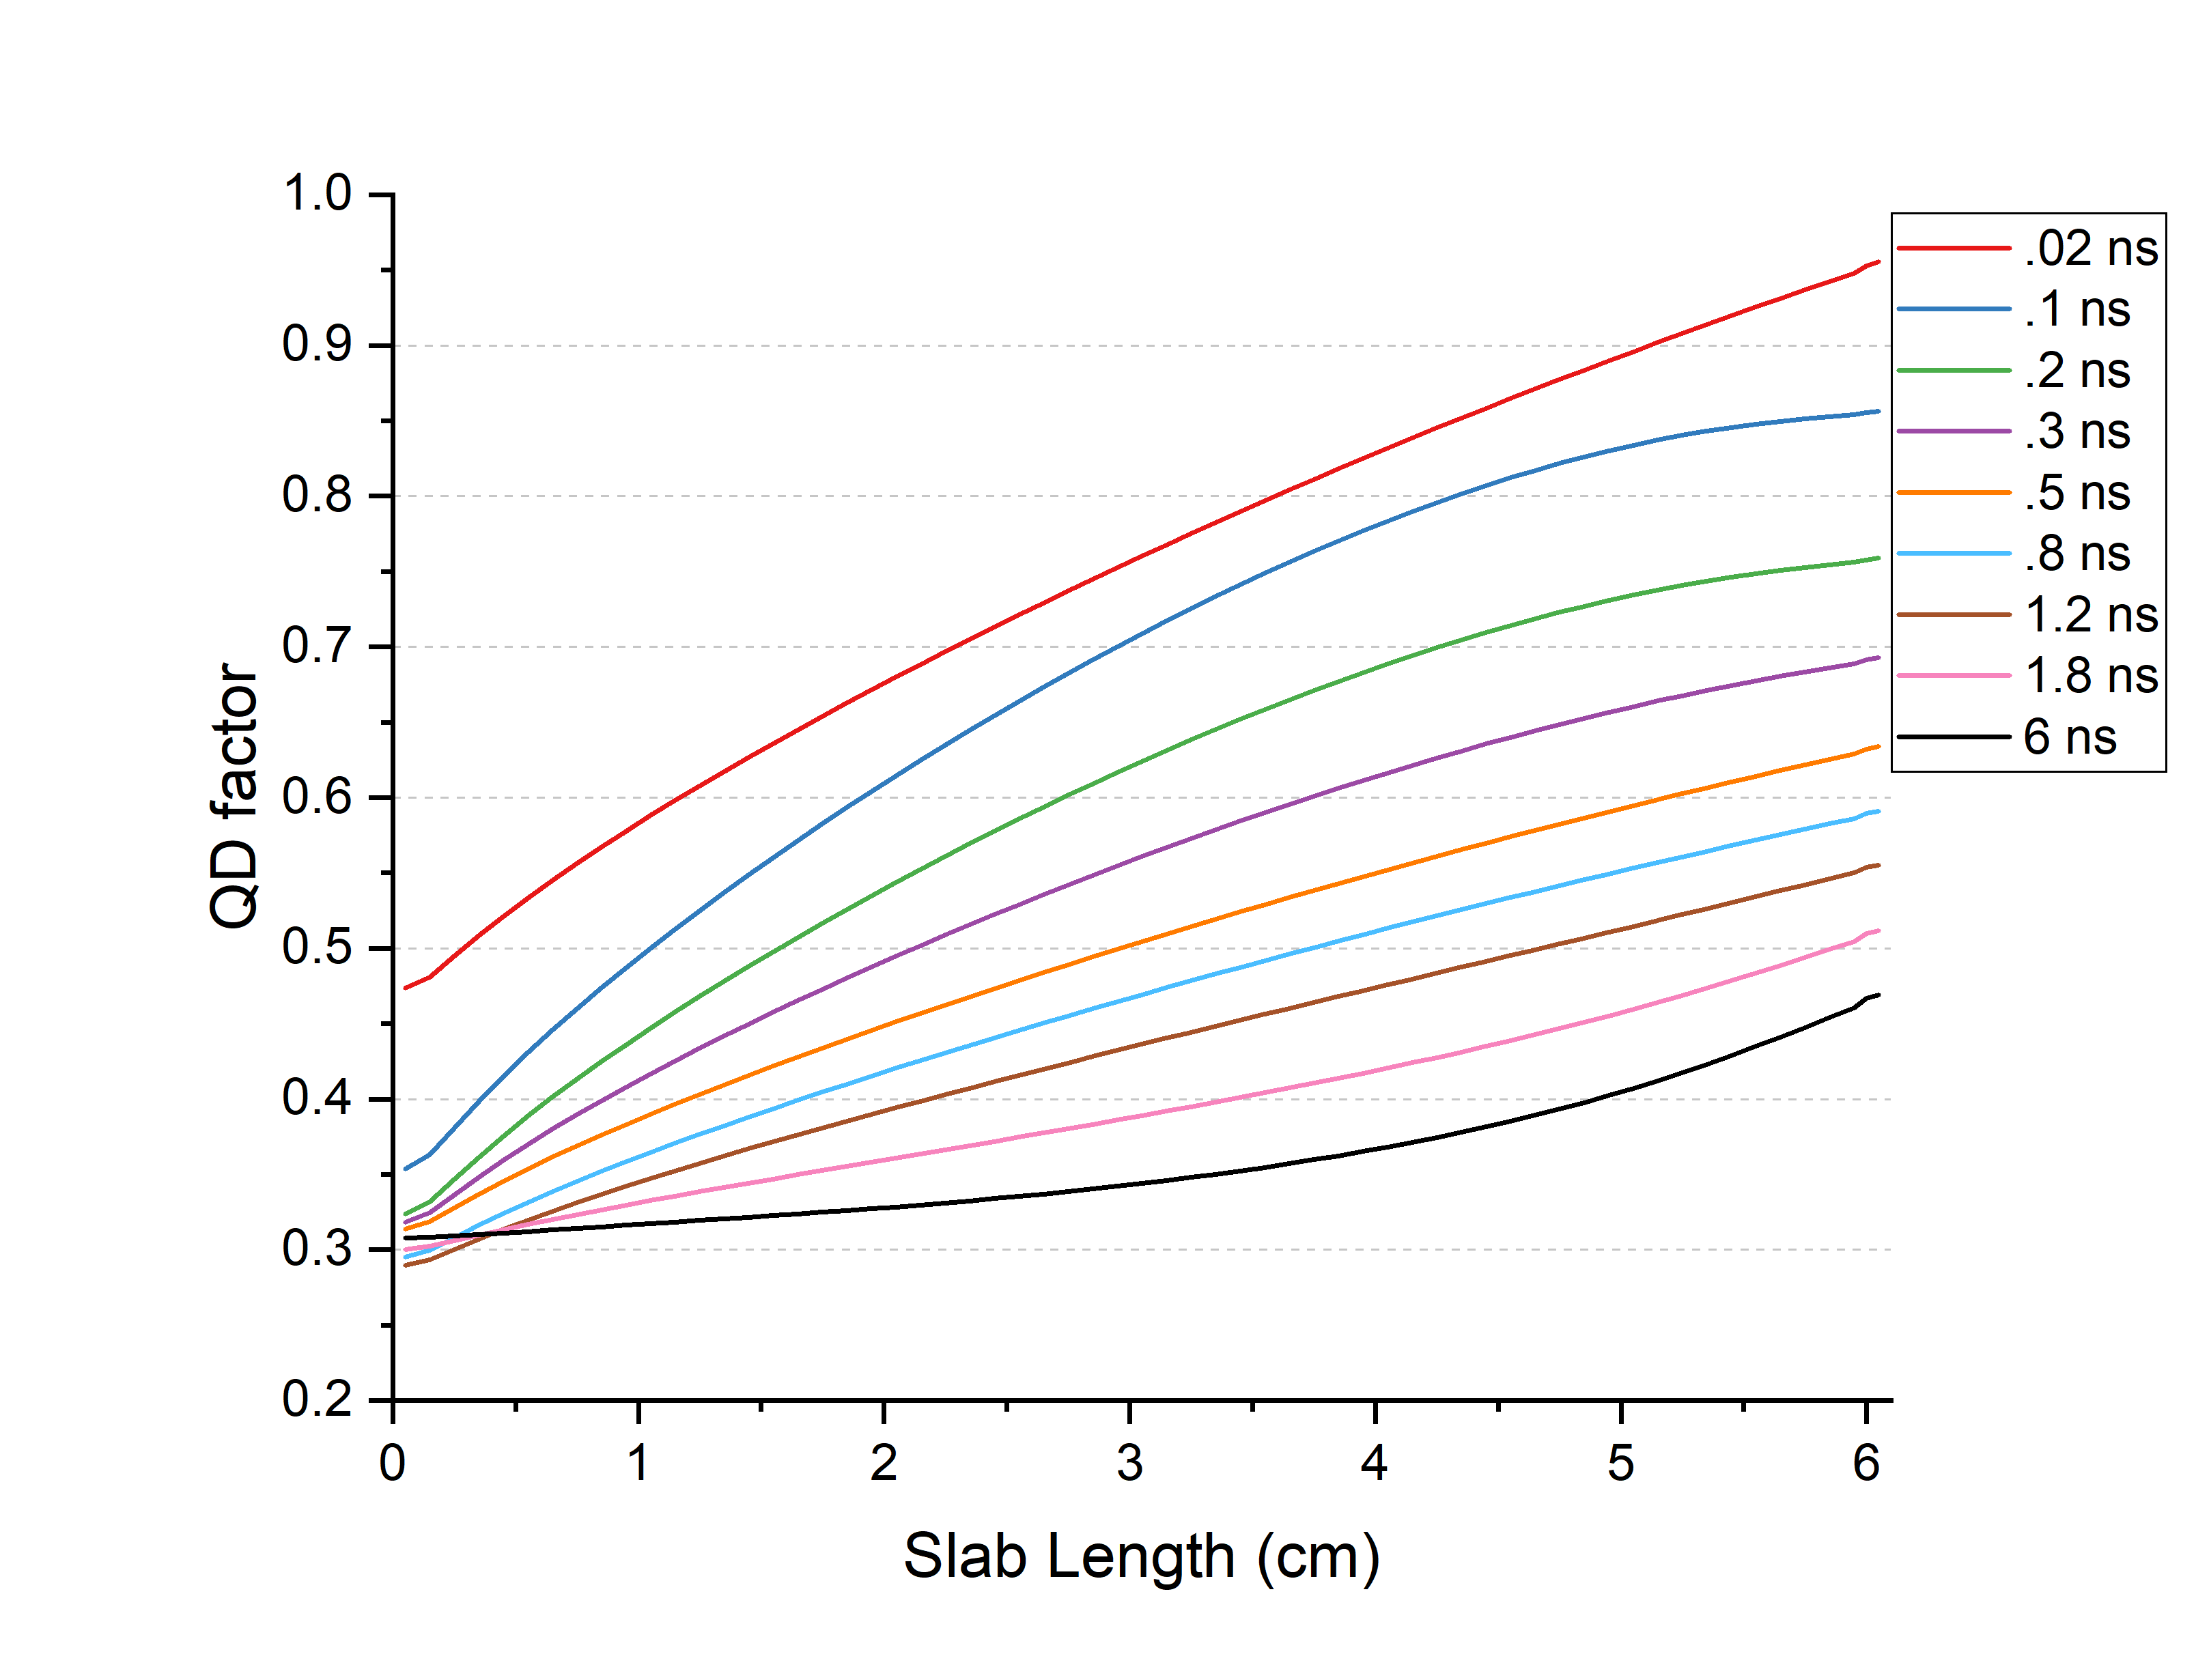
\includegraphics[width=0.5\textwidth]{qdf_g8_cut2.png}}\\
		\subfloat[r = 5 \label{subfig:qdf_g8_cut5}]{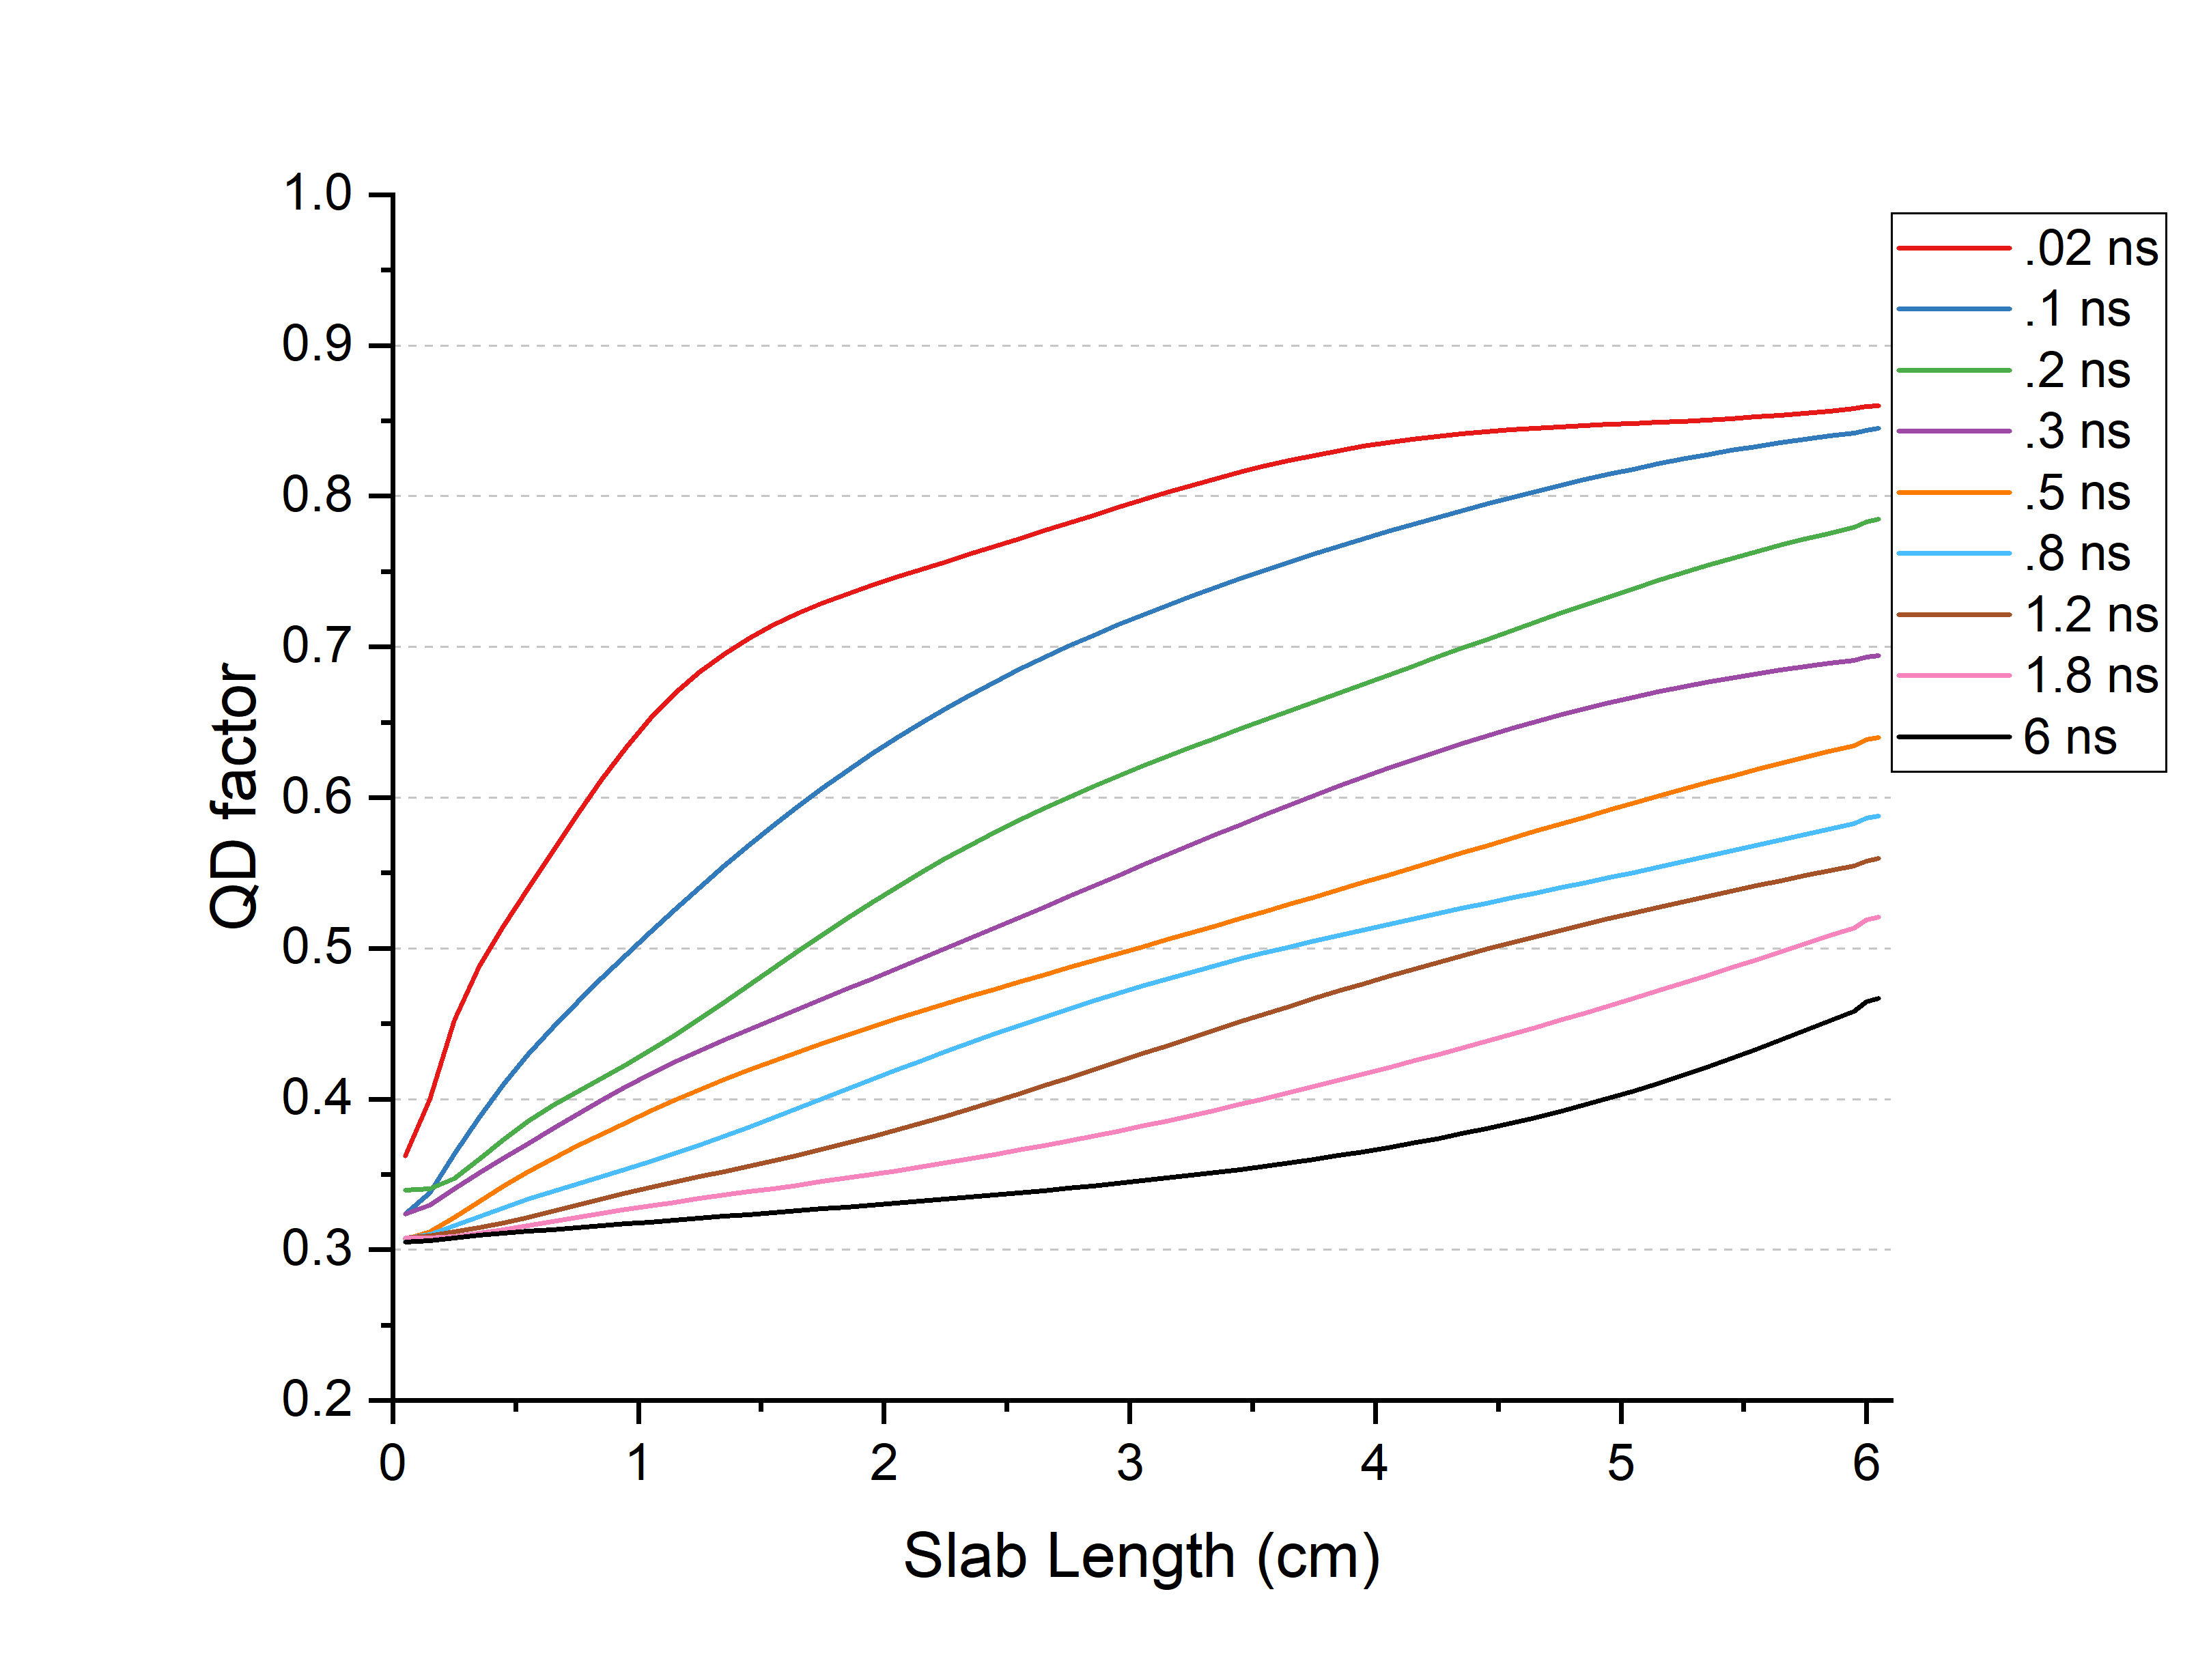
\includegraphics[width=0.5\textwidth]{qdf_g8_cut5.png}}
		\subfloat[r = 10 \label{subfig:qdf_g8_cut10}]{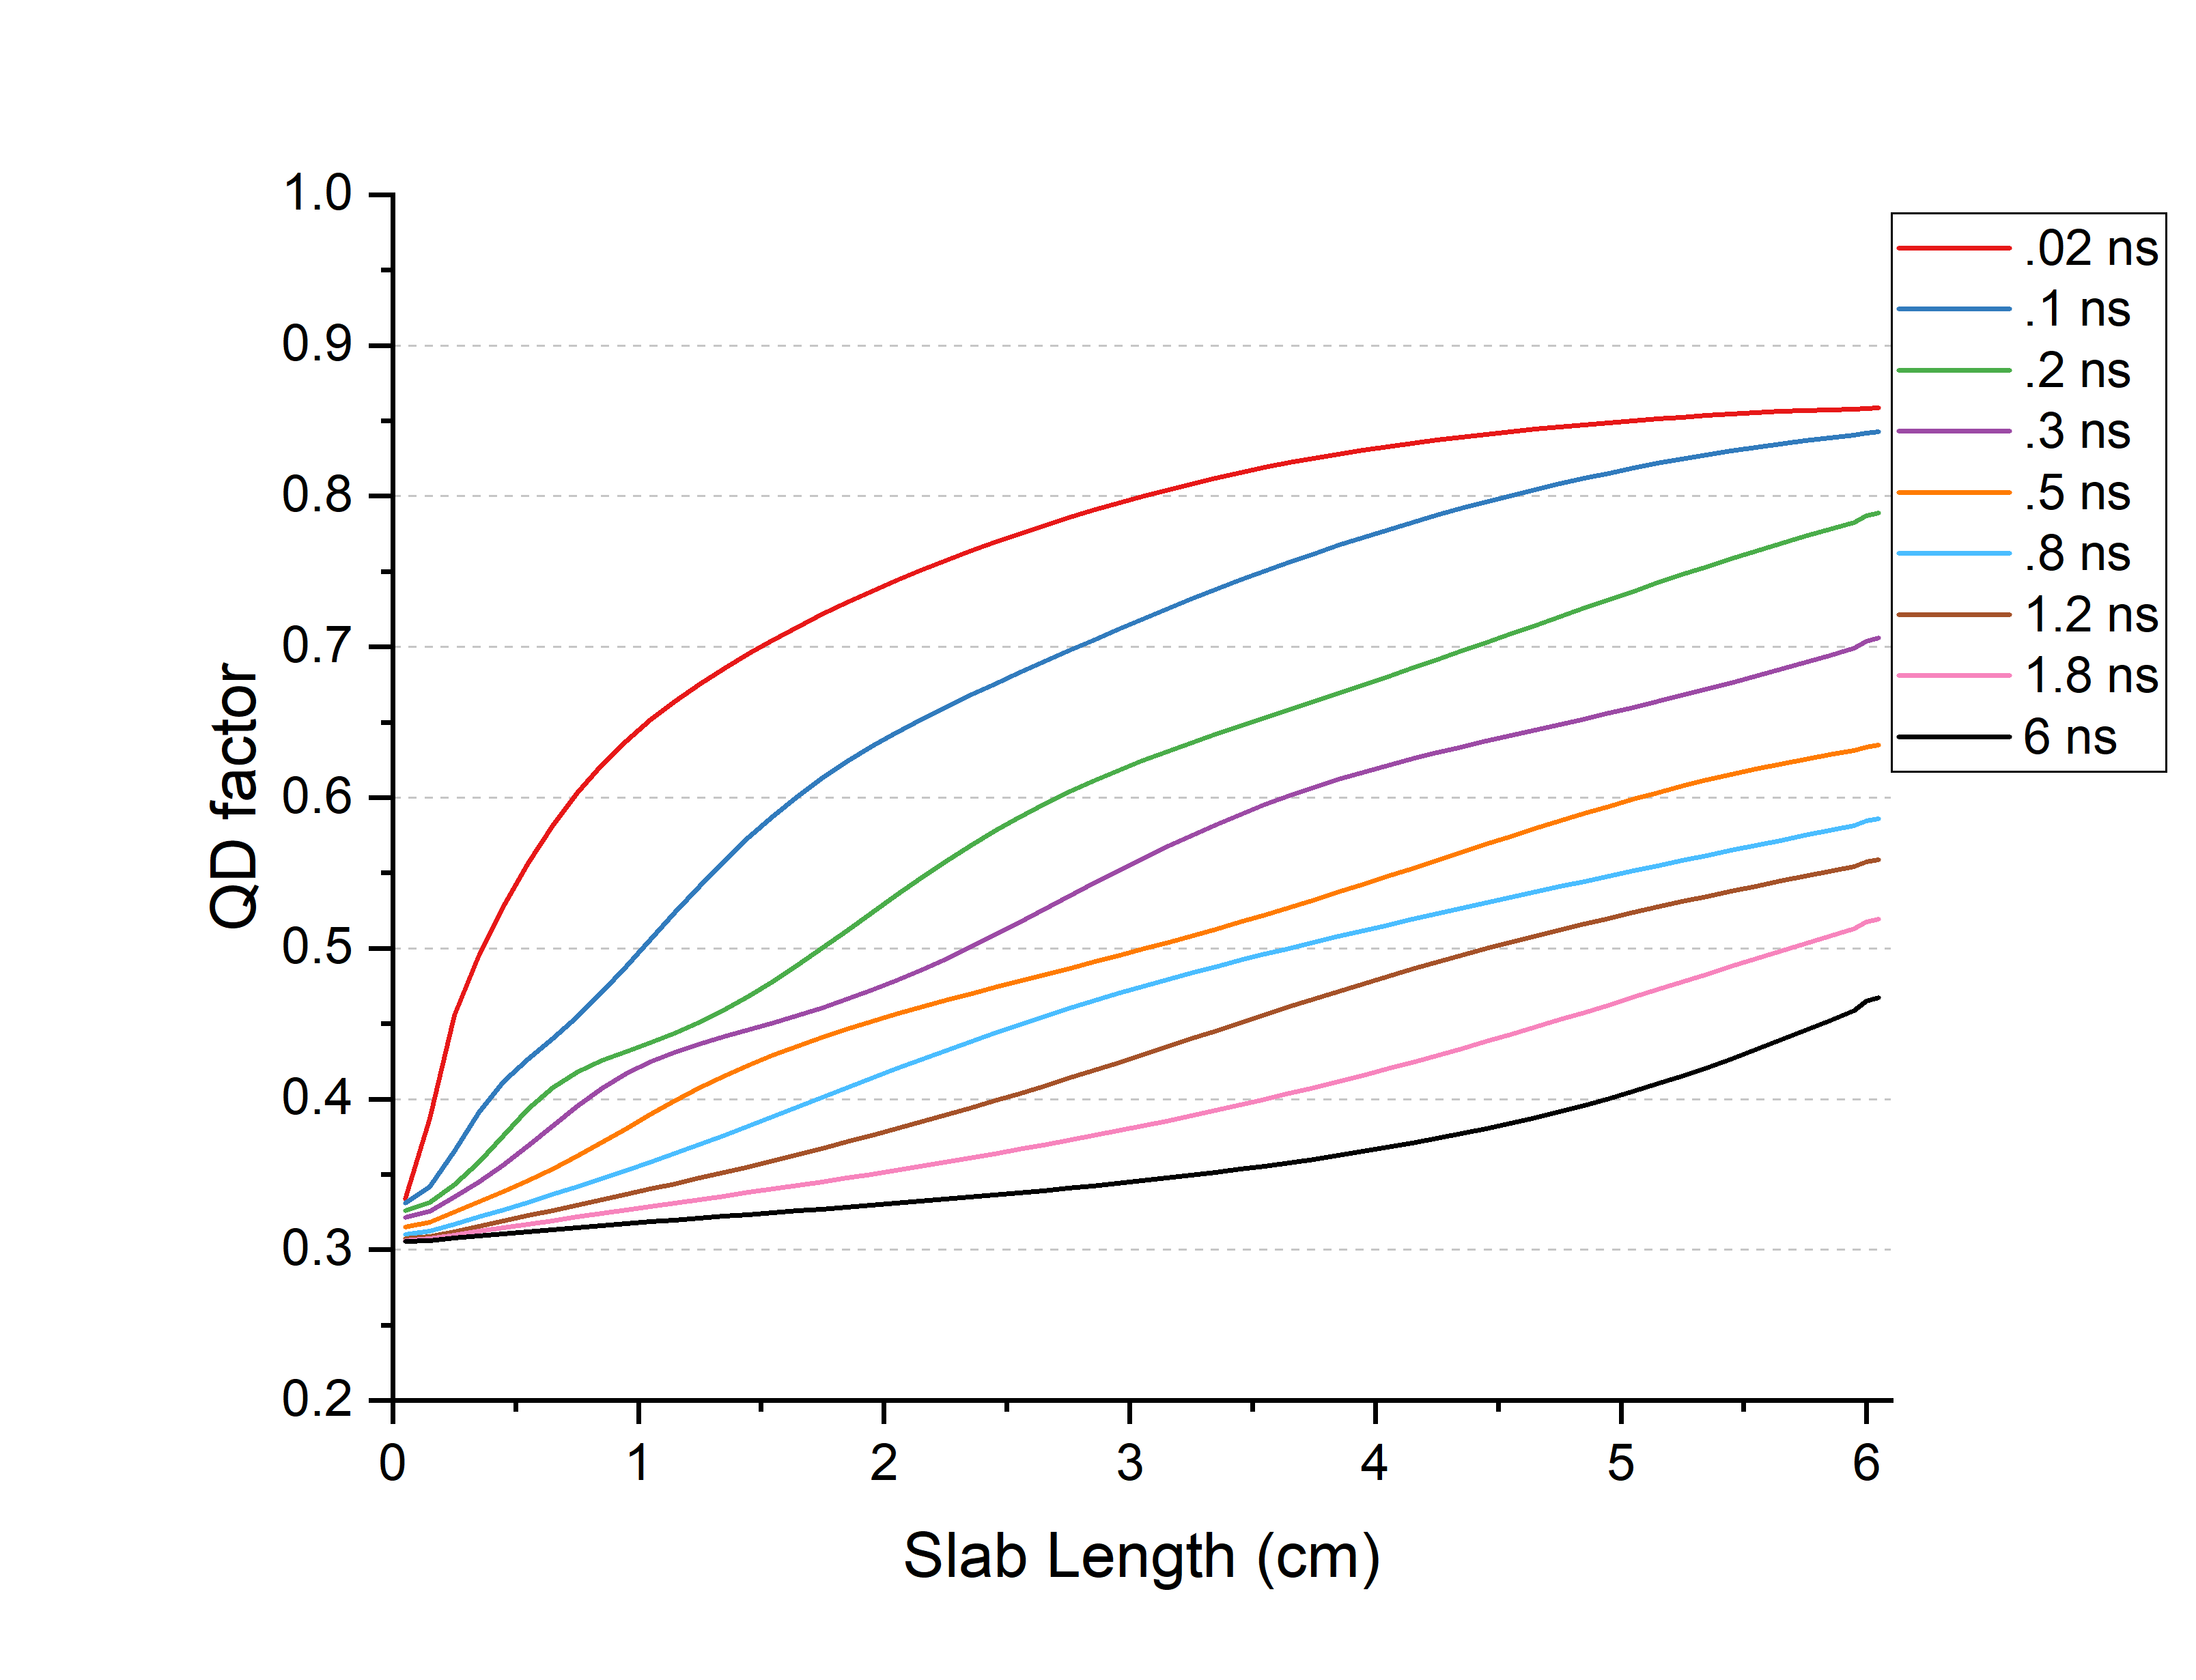
\includegraphics[width=0.5\textwidth]{qdf_g8_cut10.png}}\\
		\subfloat[r = 15 \label{subfig:qdf_g8_cut15}]{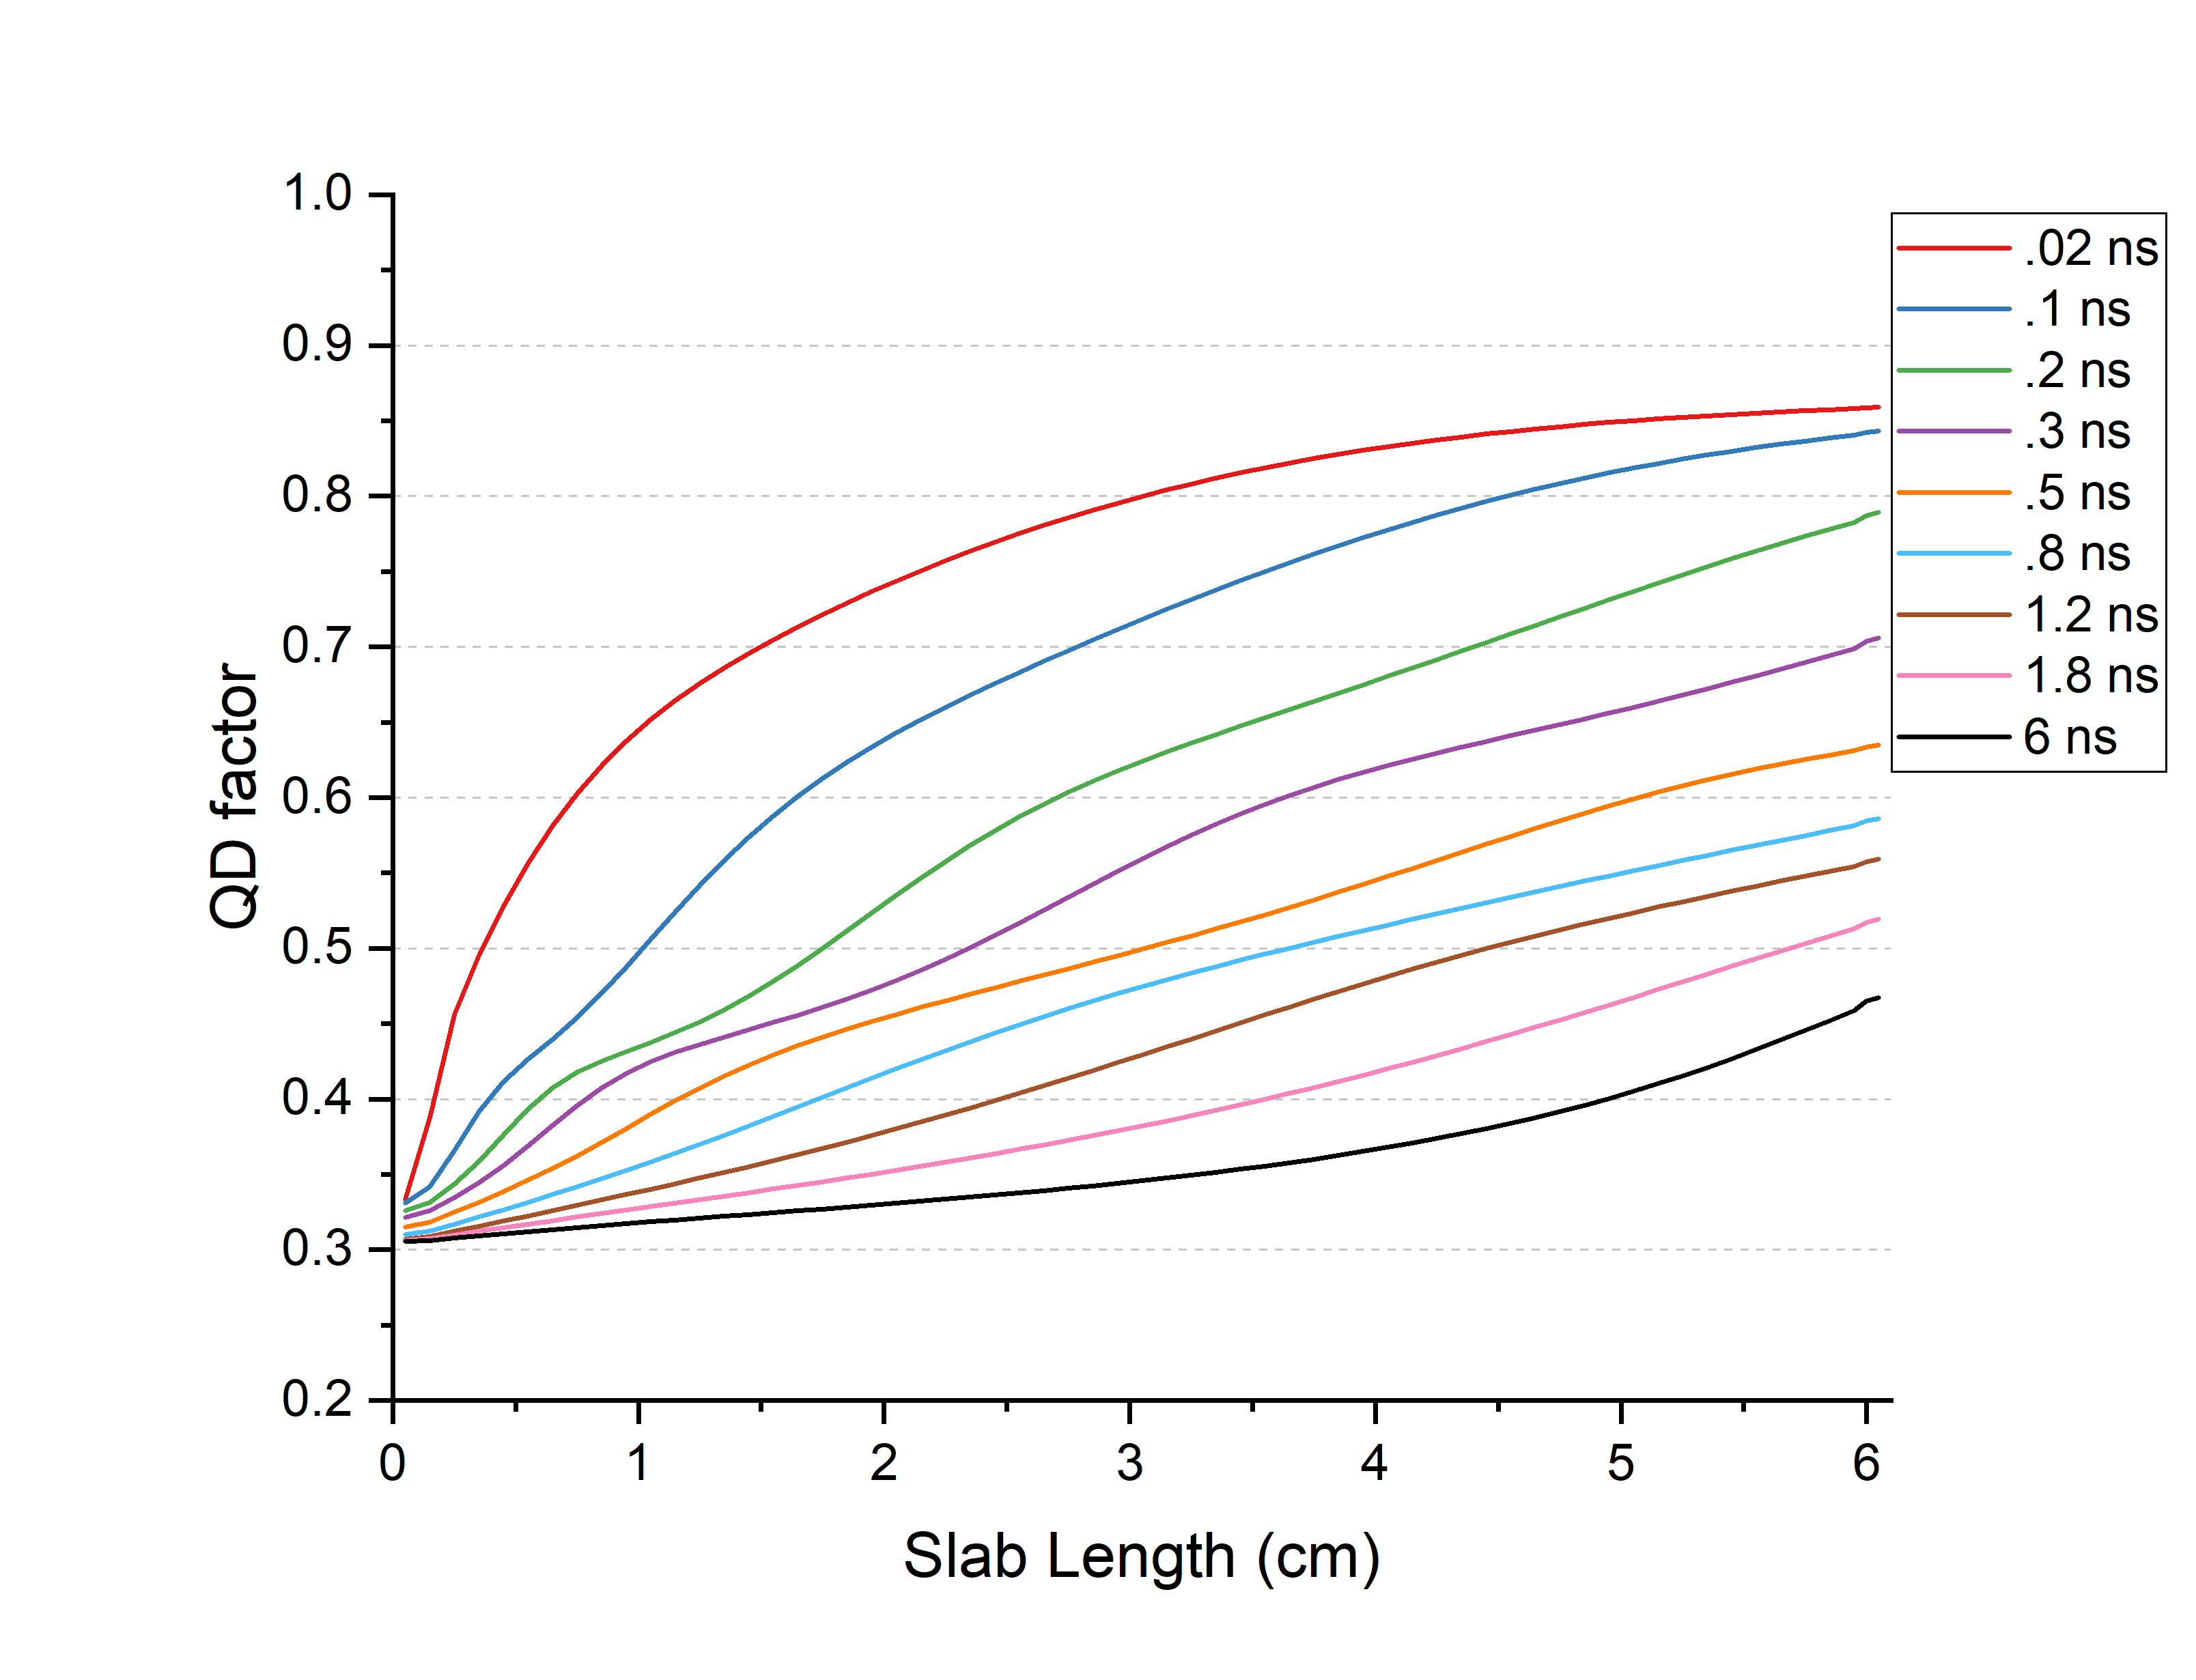
\includegraphics[width=0.5\textwidth]{qdf_g8_cut15.png}}
		\subfloat[r = 20 \label{subfig:qdf_g8_cut20}]{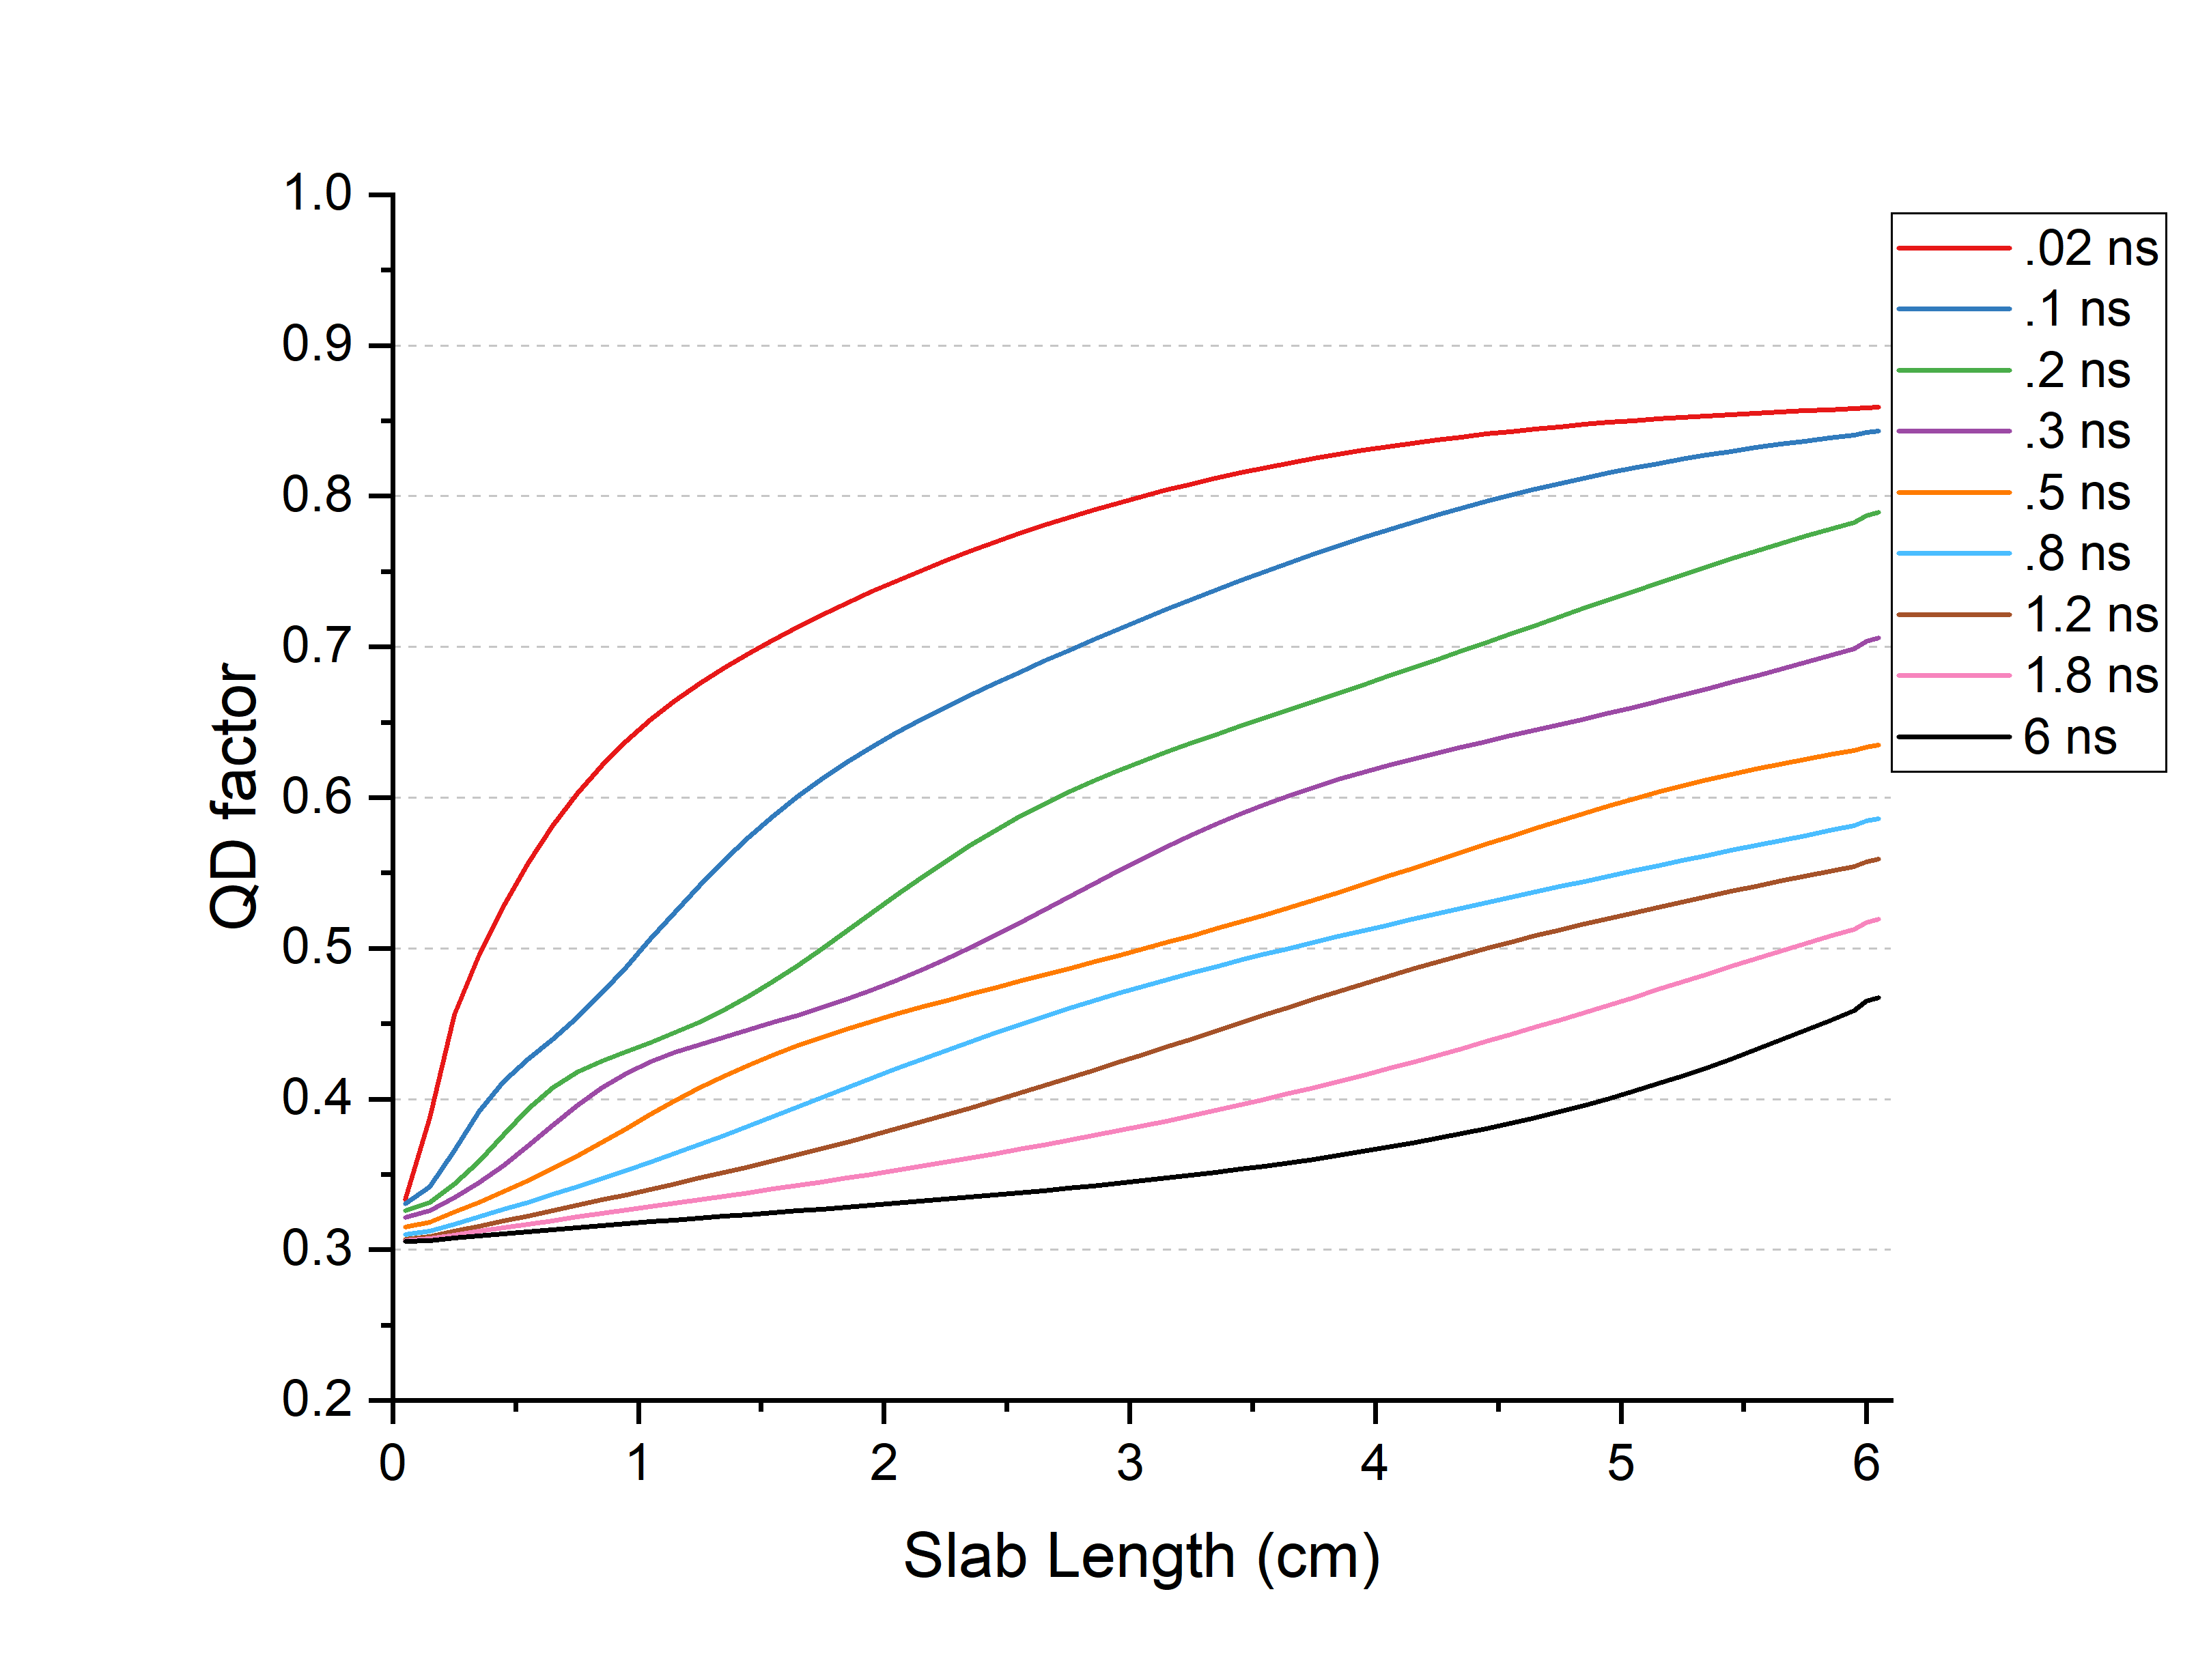
\includegraphics[width=0.5\textwidth]{qdf_g8_cut20.png}}
		\caption{\label{fig:qdf_g8_recomps}
			Low-rank approximation of the group QD factors for $g=8$ for select time steps}
	\end{figure}

\section{Numerical Results of the MLOQD-POD ROM} \label{sec:mloqd-pod_res}
	\ind The F-C test (Sec. \ref{sec:mpod_test}) is solved with the MLOQD-POD ROM for $0 \le t  \le 6$ ns using  the time step length $\Delta t=2 \times 10^{-2}$ ns. Thus, there are 300 time steps. This is the number of snapshots used to build the data set of reference QD factors. We consider MLOQD-POD ROMs using singular value relative cutoff criteria of $\varepsilon_\sigma = 10^{-1}, 10^{-2}, \dots 10^{-12}$. Figure \ref{fig:ref_errs_inf} presents the relative error of the solution of these MLOQD-POD ROMs compared to the  reference solution in the  $\infty$-norm at every instant of time. The results show how the accuracy of MLOQD-POD ROMs improves as $\varepsilon_\sigma$  decreases. The relative error is decreases in magnitude at every instant of time for both temperature and energy density for each successive decrease of $\varepsilon_\sigma$. Note that  both temperature and energy density obtained by means of these MLOQD-POQ ROMs eventually match the reference solution, as the relative error reaches the level of convergence specified for the test problem $\pr{\epsilon_T=\epsilon_E=10^{-12}}$.

	%=================================================================================
	% TEST PROBLEM ERRORS
	\begin{figure}[ht!]
		\centering
		\subfloat[Temperature relative error \label{subfig:refcase_Temp_rel_inf}]{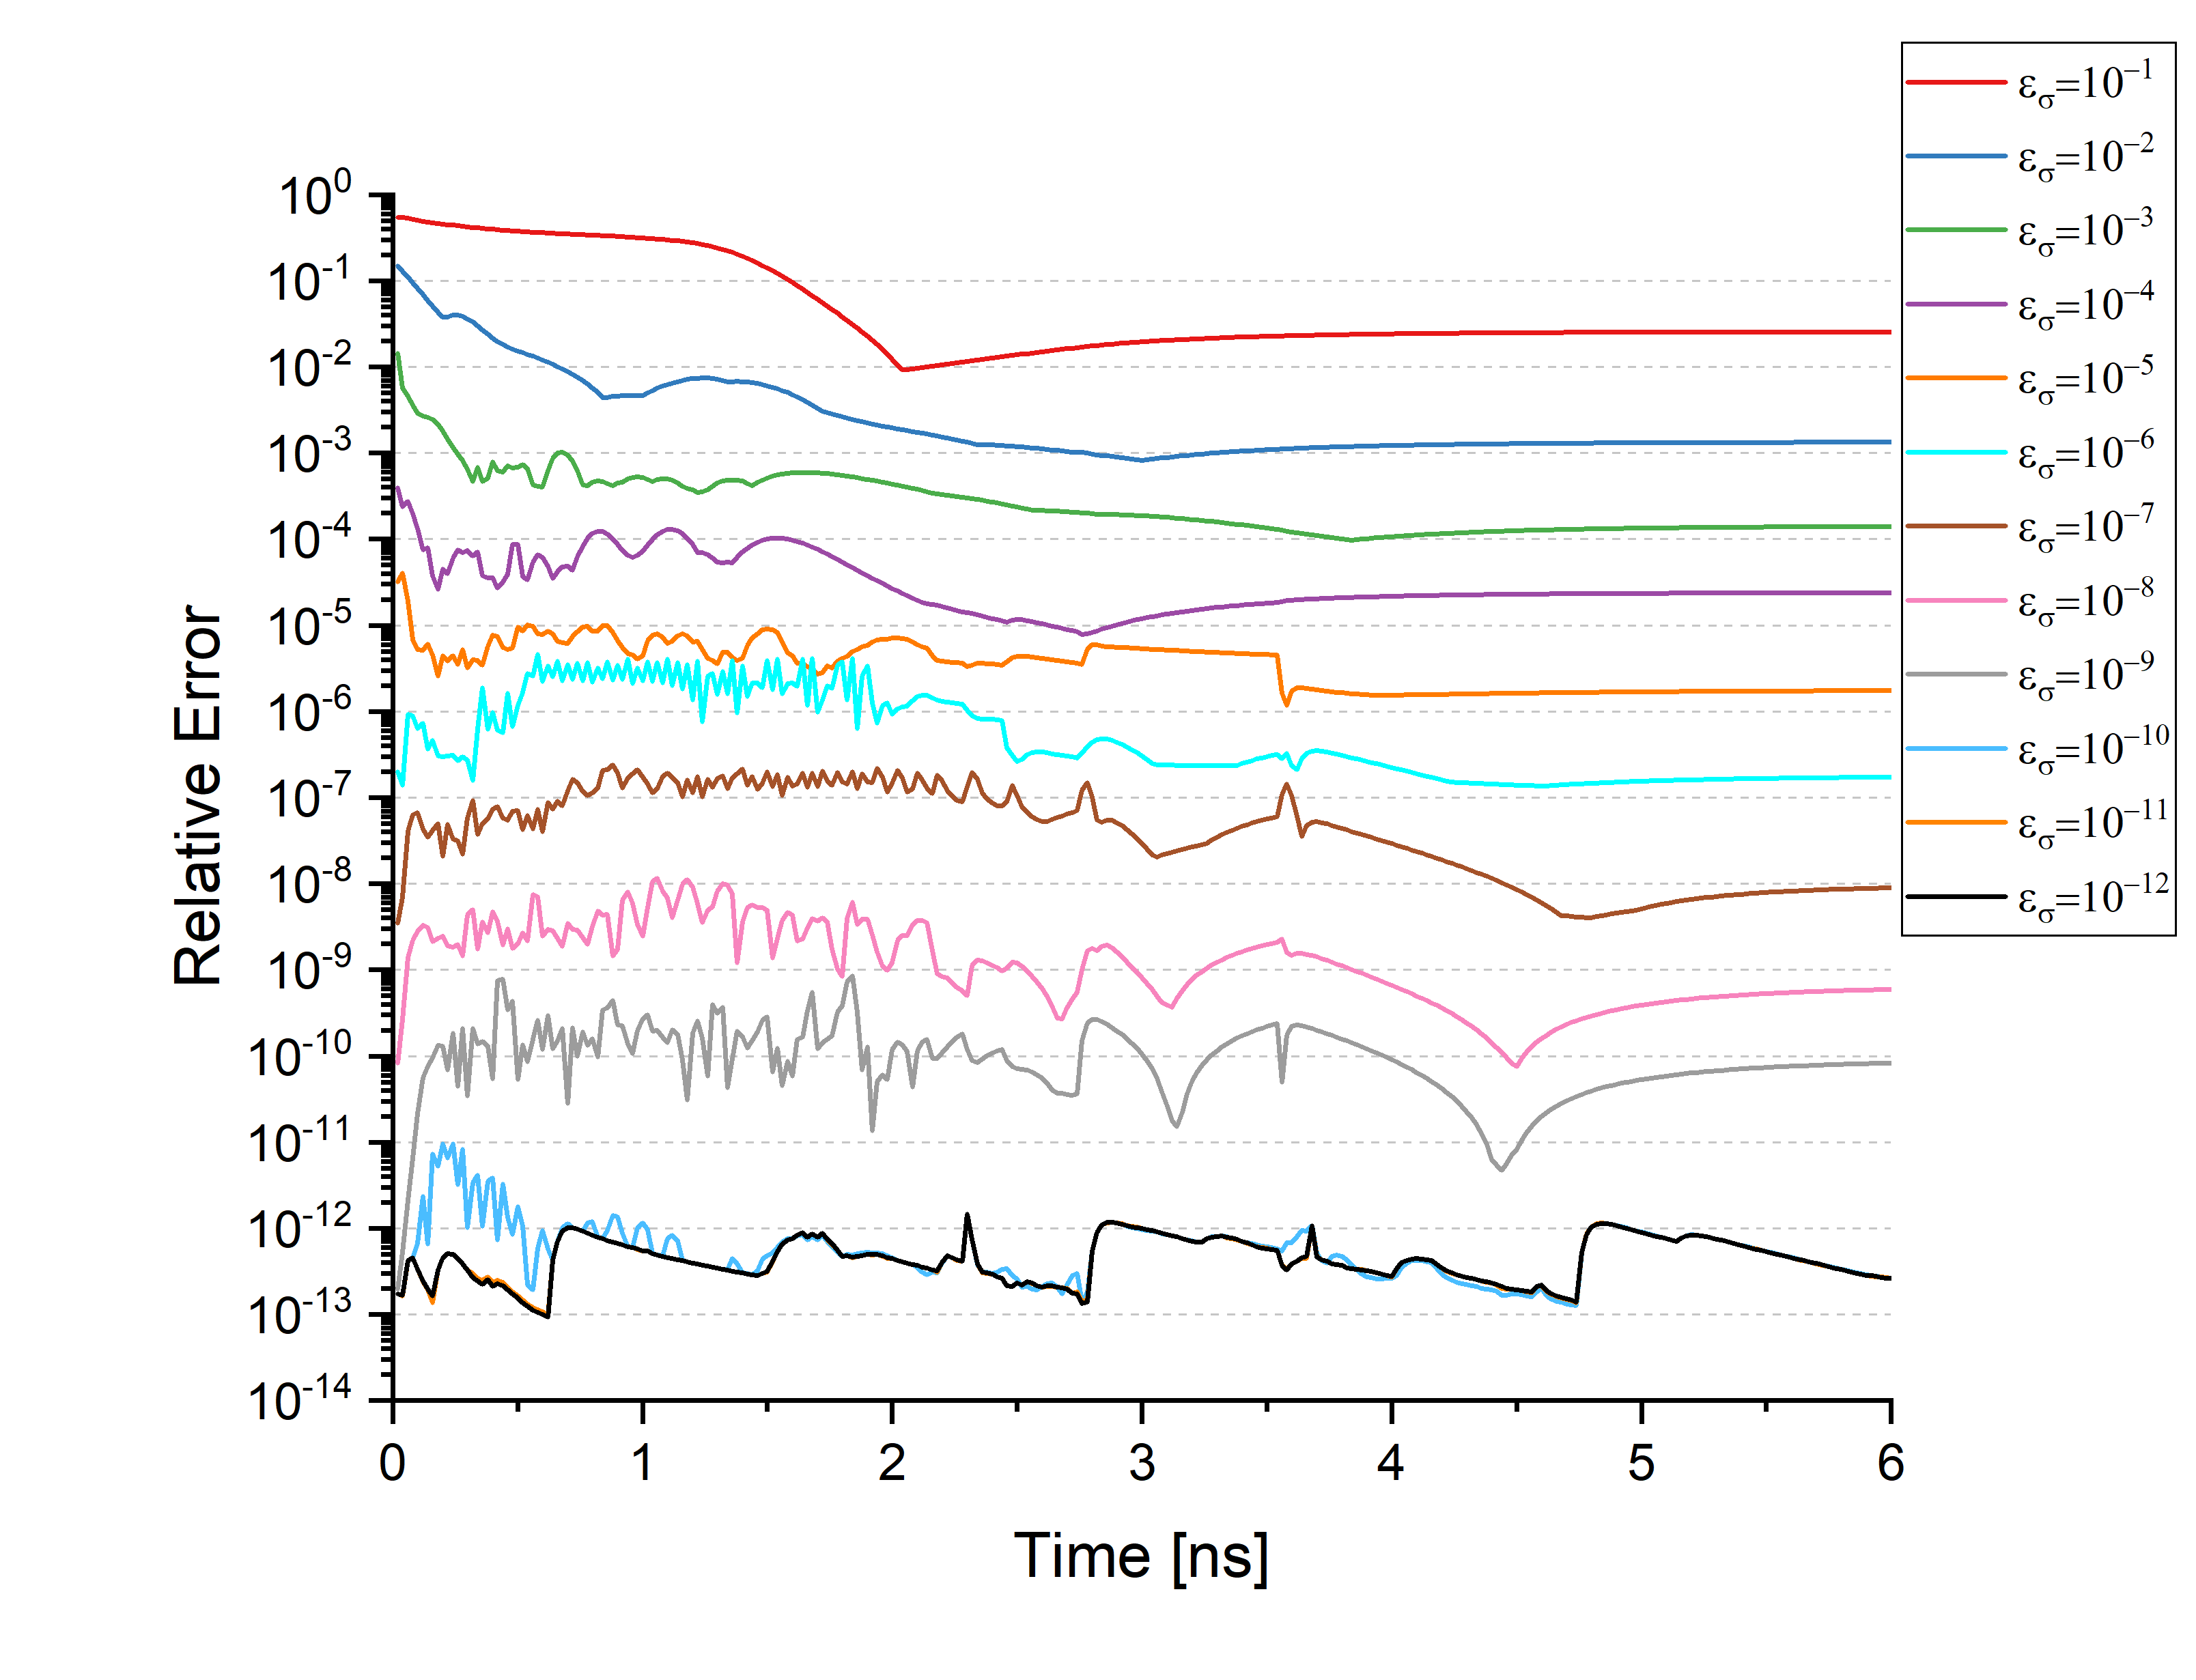
\includegraphics[width=0.5\textwidth]{refcase_Temp_rel_inf.png}}
		\subfloat[Total energy density relative error \label{subfig:refcase_E_rel_inf}]{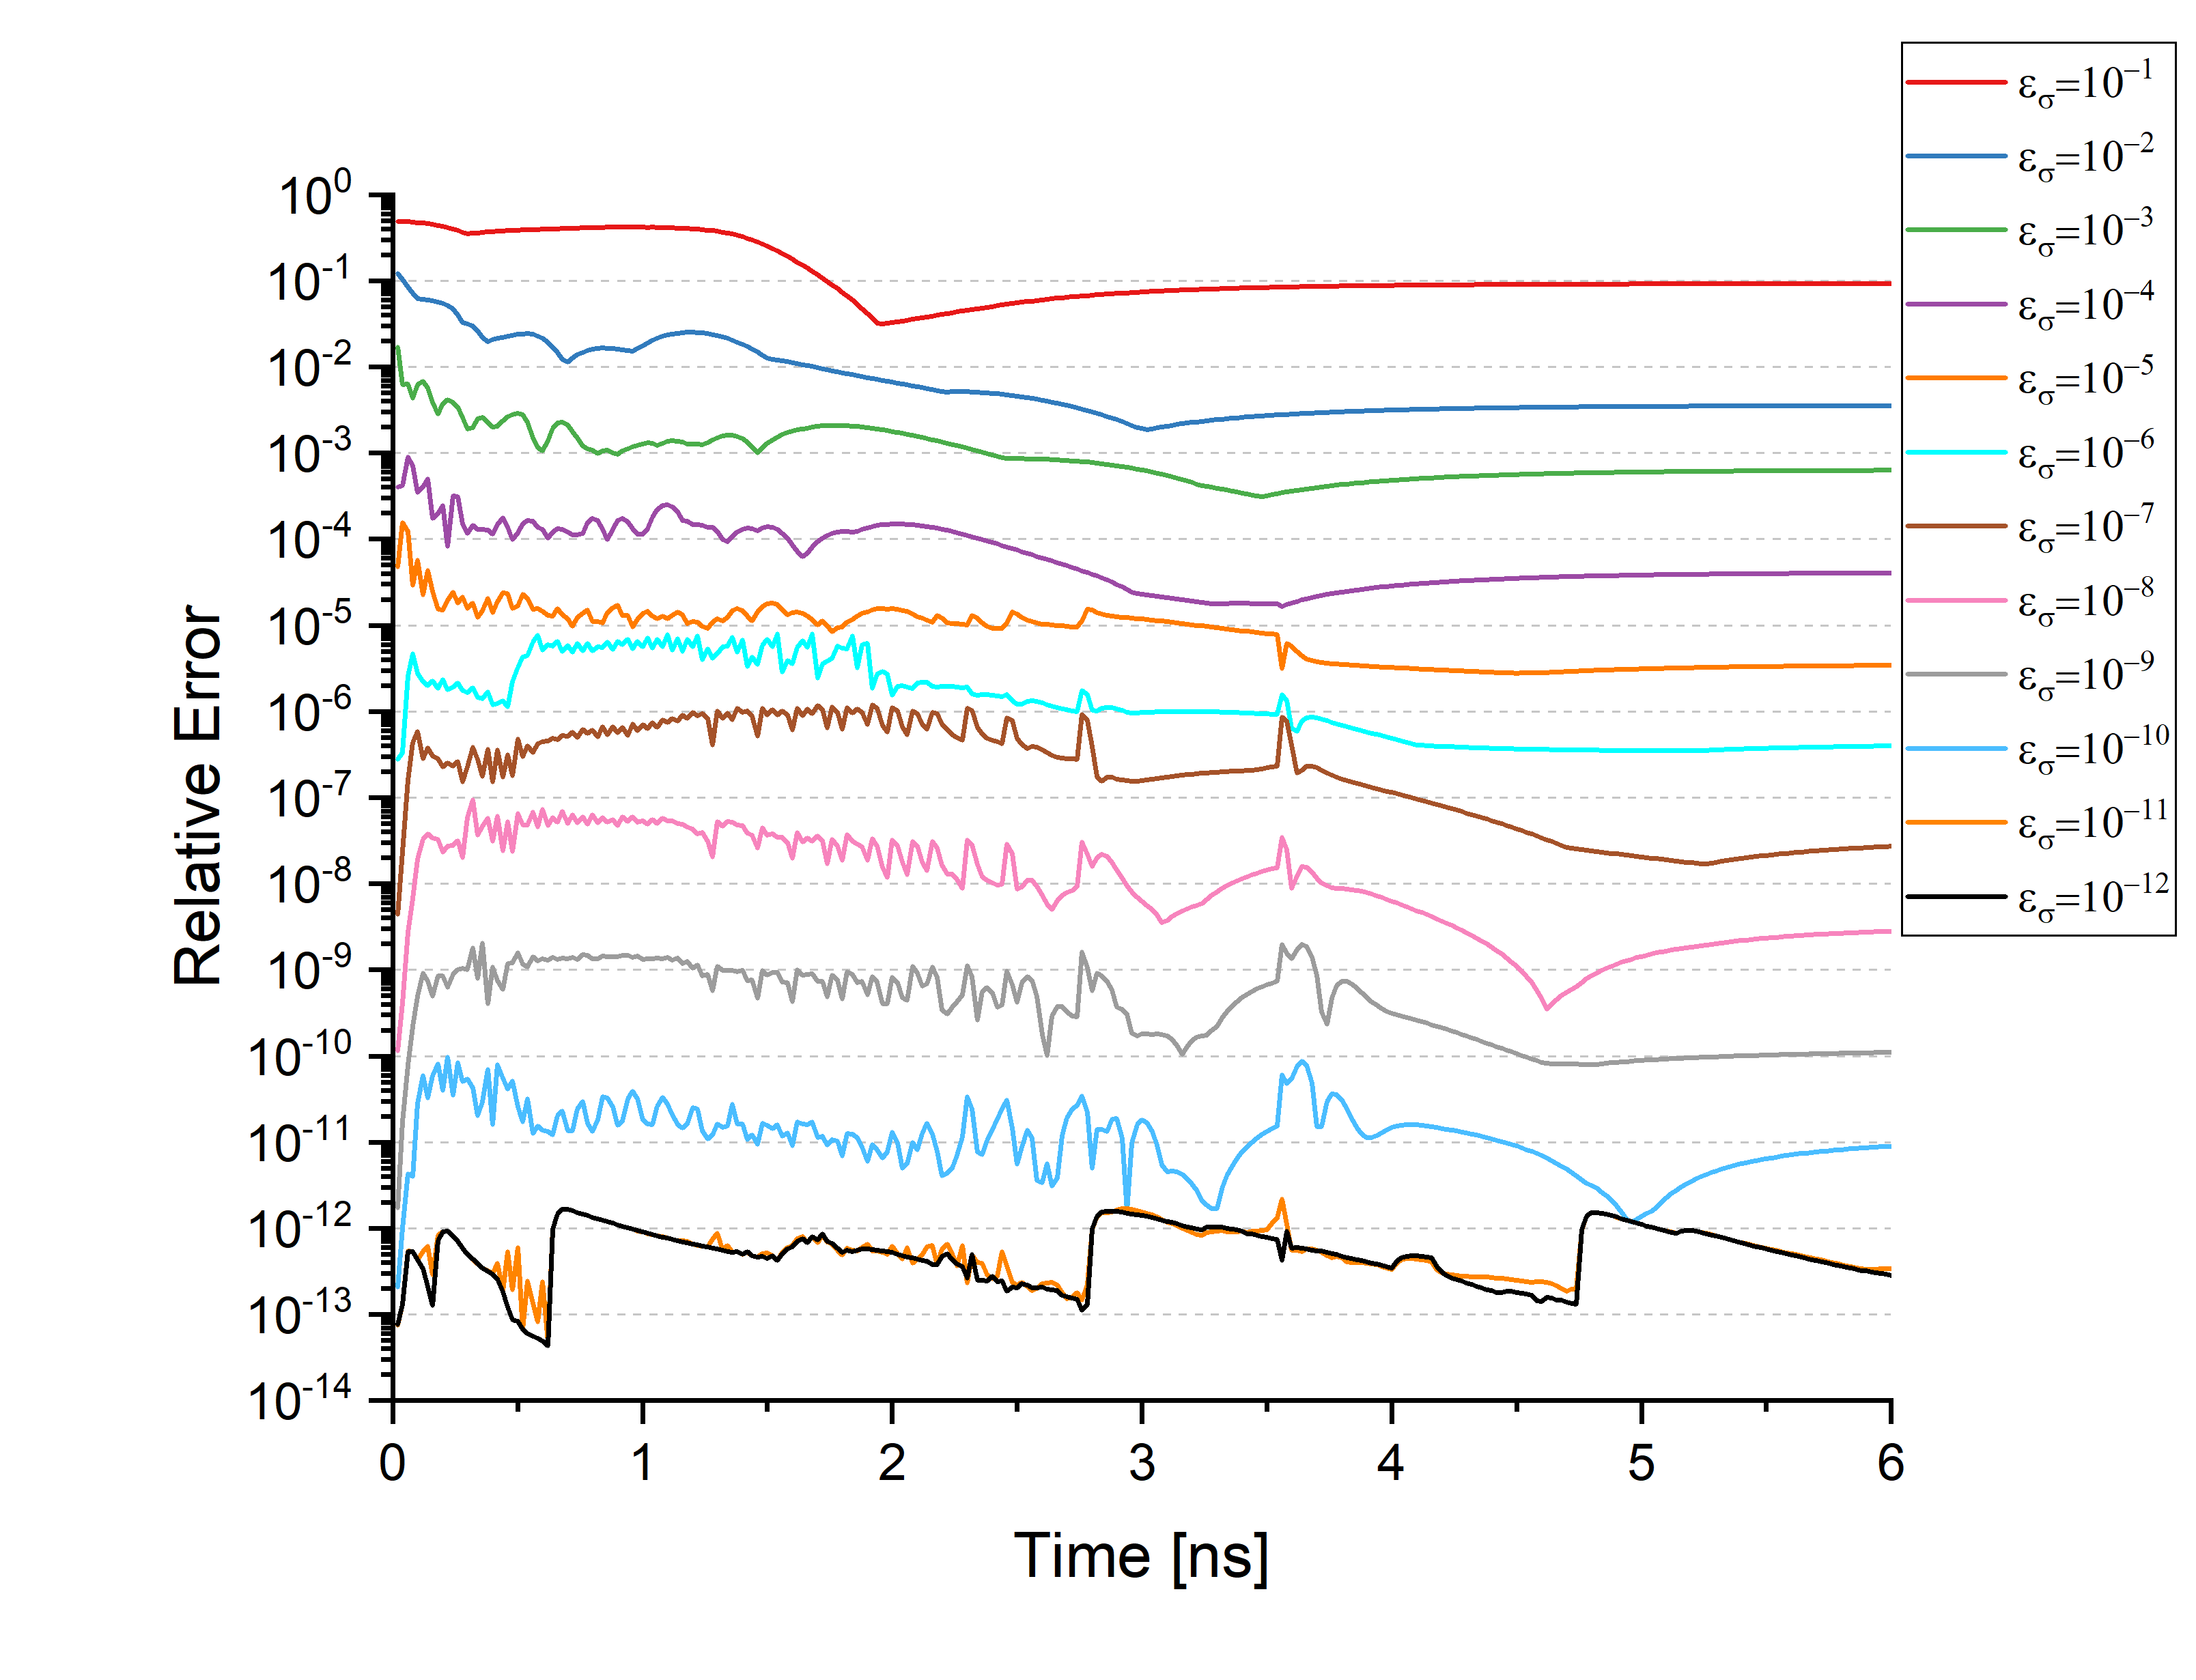
\includegraphics[width=0.5\textwidth]{refcase_E_rel_inf.png}}
		\caption{\label{fig:ref_errs_inf}
			Relative Error of the MLOQD-POD ROM solution to the F-C test problem versus the high order solution in $\infty$ norm for various $\varepsilon_\sigma$ values}
	\end{figure}

	\ind The MLOQD-POD ROM also has the capability to use an incomplete database of QD factors. For instance, using the database formed for the original F-C test described in Sec. \ref{sec:mpod_test} the MLOQD-POD ROM may solve the F-C test with a refined time step length. In this case the problem is solved over more instants of time than are included in the database. QD factors for the instants of time not included in the database are calculated with linear interpolation between the recorded values \cite{Bui-Thanh-2003}. Figure \ref{fig:errors_dt-0.01} shows the  relative error in $L_1$-norm of the MLOQD-POD ROM solution computed with $\Delta t \! = \! 1\! \times\! 10^{-2}$ ns using various values of $\varepsilon_{\sigma}$. Figure \ref{fig:errors_dt-0.005}  presents the relative error in $L_1$-norm of the solutions computed with $\Delta t \! = \! 5\! \times  \! 10^{-3}$ ns. Figure \ref{fig:errors_dt-0.002}  presents the relative error in $L_1$-norm of the solutions computed with $\Delta t \! = \! 2\! \times  \! 10^{-3}$ ns. The reference solution is recalculated for each time step length to find relative errors, and the database generated with $\Delta t = 2\times 10^{-2}$ ns is used for all MLOQD-POD ROMs. The relative error of these MLOQD-POD ROMs saturates at $\varepsilon_\sigma=10^{-4}$, thus the shown results are for only $\varepsilon_\sigma \geq 10^{-4}$. For all cases the error at the early time steps is large and drops several orders of magnitude as the problem progresses, which can be attributed to how the dynamics of the problem evolve. The radiation front changes most rapidly at the start of the problem during initial wave formation. The group QD factors experience similarly rapid changes as a result as depicted in Figs. \ref{fig:qdf_g2_recomps}, \ref{fig:qdf_g3_recomps} and \ref{fig:qdf_g8_recomps}. Such swift changes may be difficult to estimate with linear interpolation, limiting the accuracy of the ROM at early times. When comparing the relative error of each ROM the error at early instants of time does not significantly change, and at the final stage of the problem when the change rate of the solution is very small there is only an order of magnitude difference in the errors between the solutions computed with time steps $1\times10^{-2}$ ns and $2\times10^{-3}$ ns. The difference in time step length between these two cases is an order of 5, thus the error of the MLOQD-POD ROM is not very sensitive to how refined the time step length is compared to the reference case from which the approximate QD factors are generated.

	%=================================================================================
	% REDUCED TIME STEP ERRORS PLOT
	\begin{figure}[ht!]
		\centering
		\subfloat[Temperature relative error \label{subfig-1:MG_bc1000-t001_qdf1000-t002_Tavg_mlqd}]{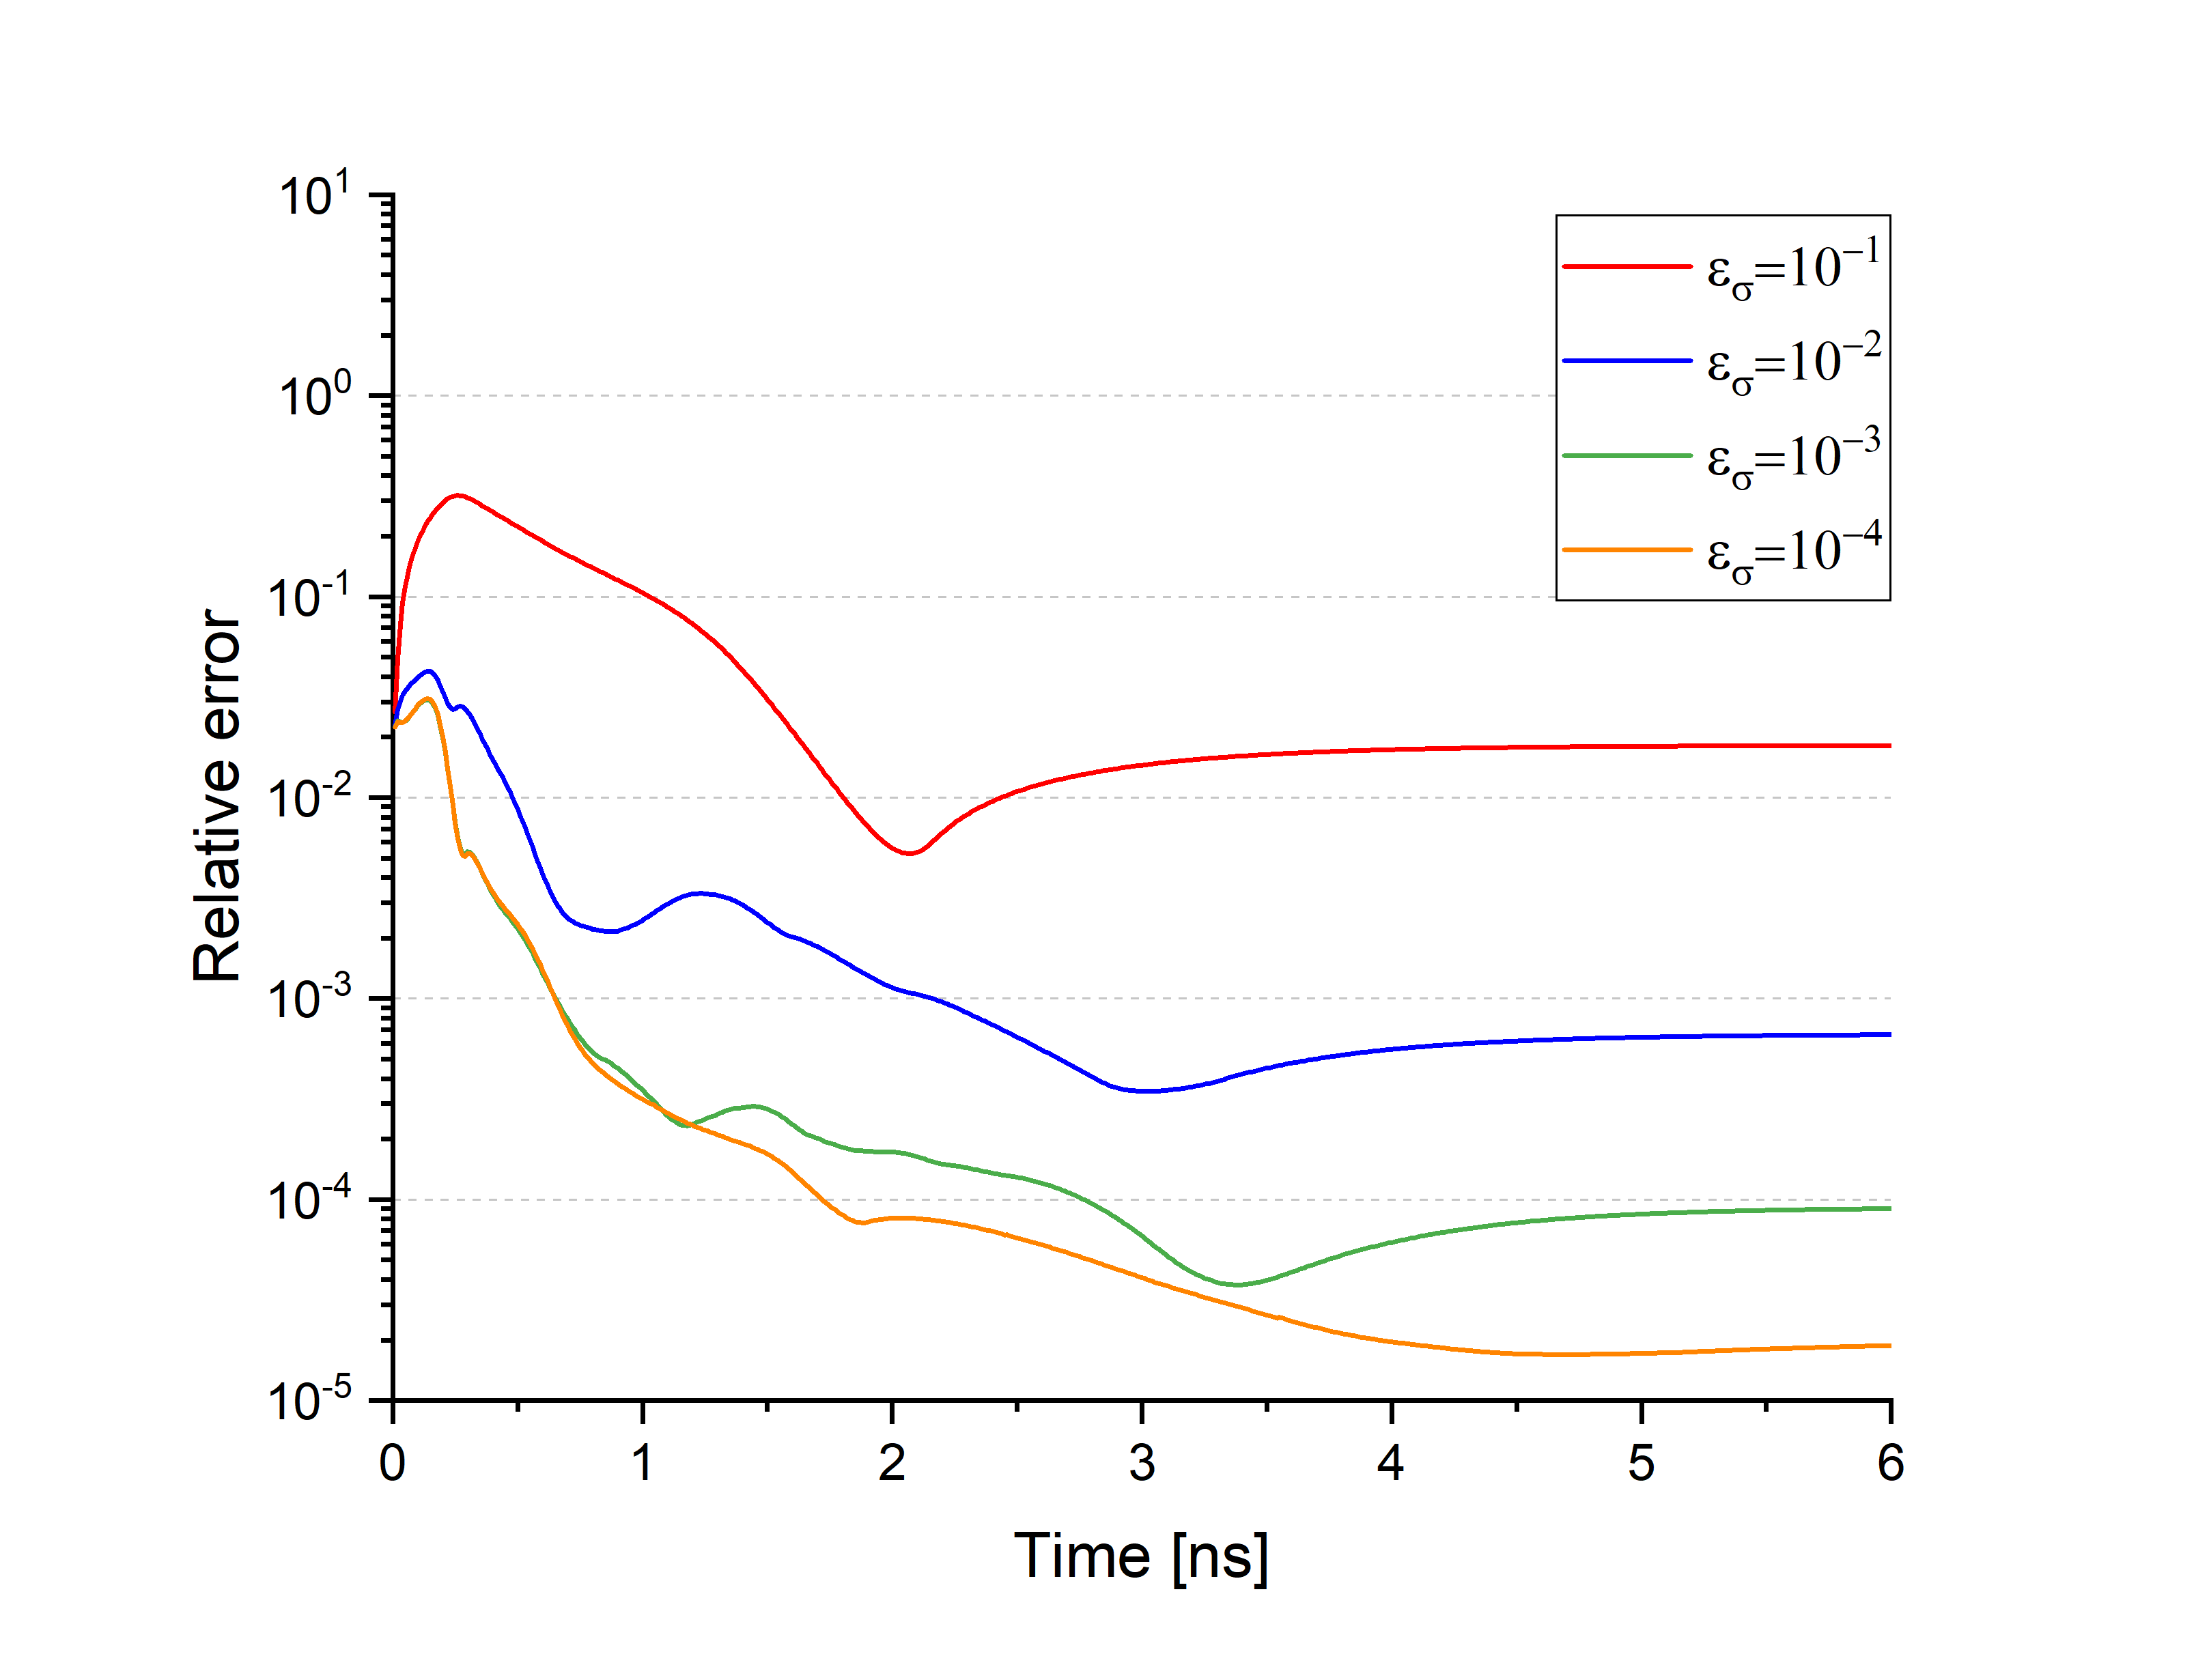
\includegraphics[width=0.5\textwidth]{MG_bc1000-t001_qdf1000-t002_Tavg_mlqd.png}}
		\subfloat[Energy density relative error \label{subfig-1:MG_bc1000-t001_qdf1000-t002_Eavg_mlqd}]{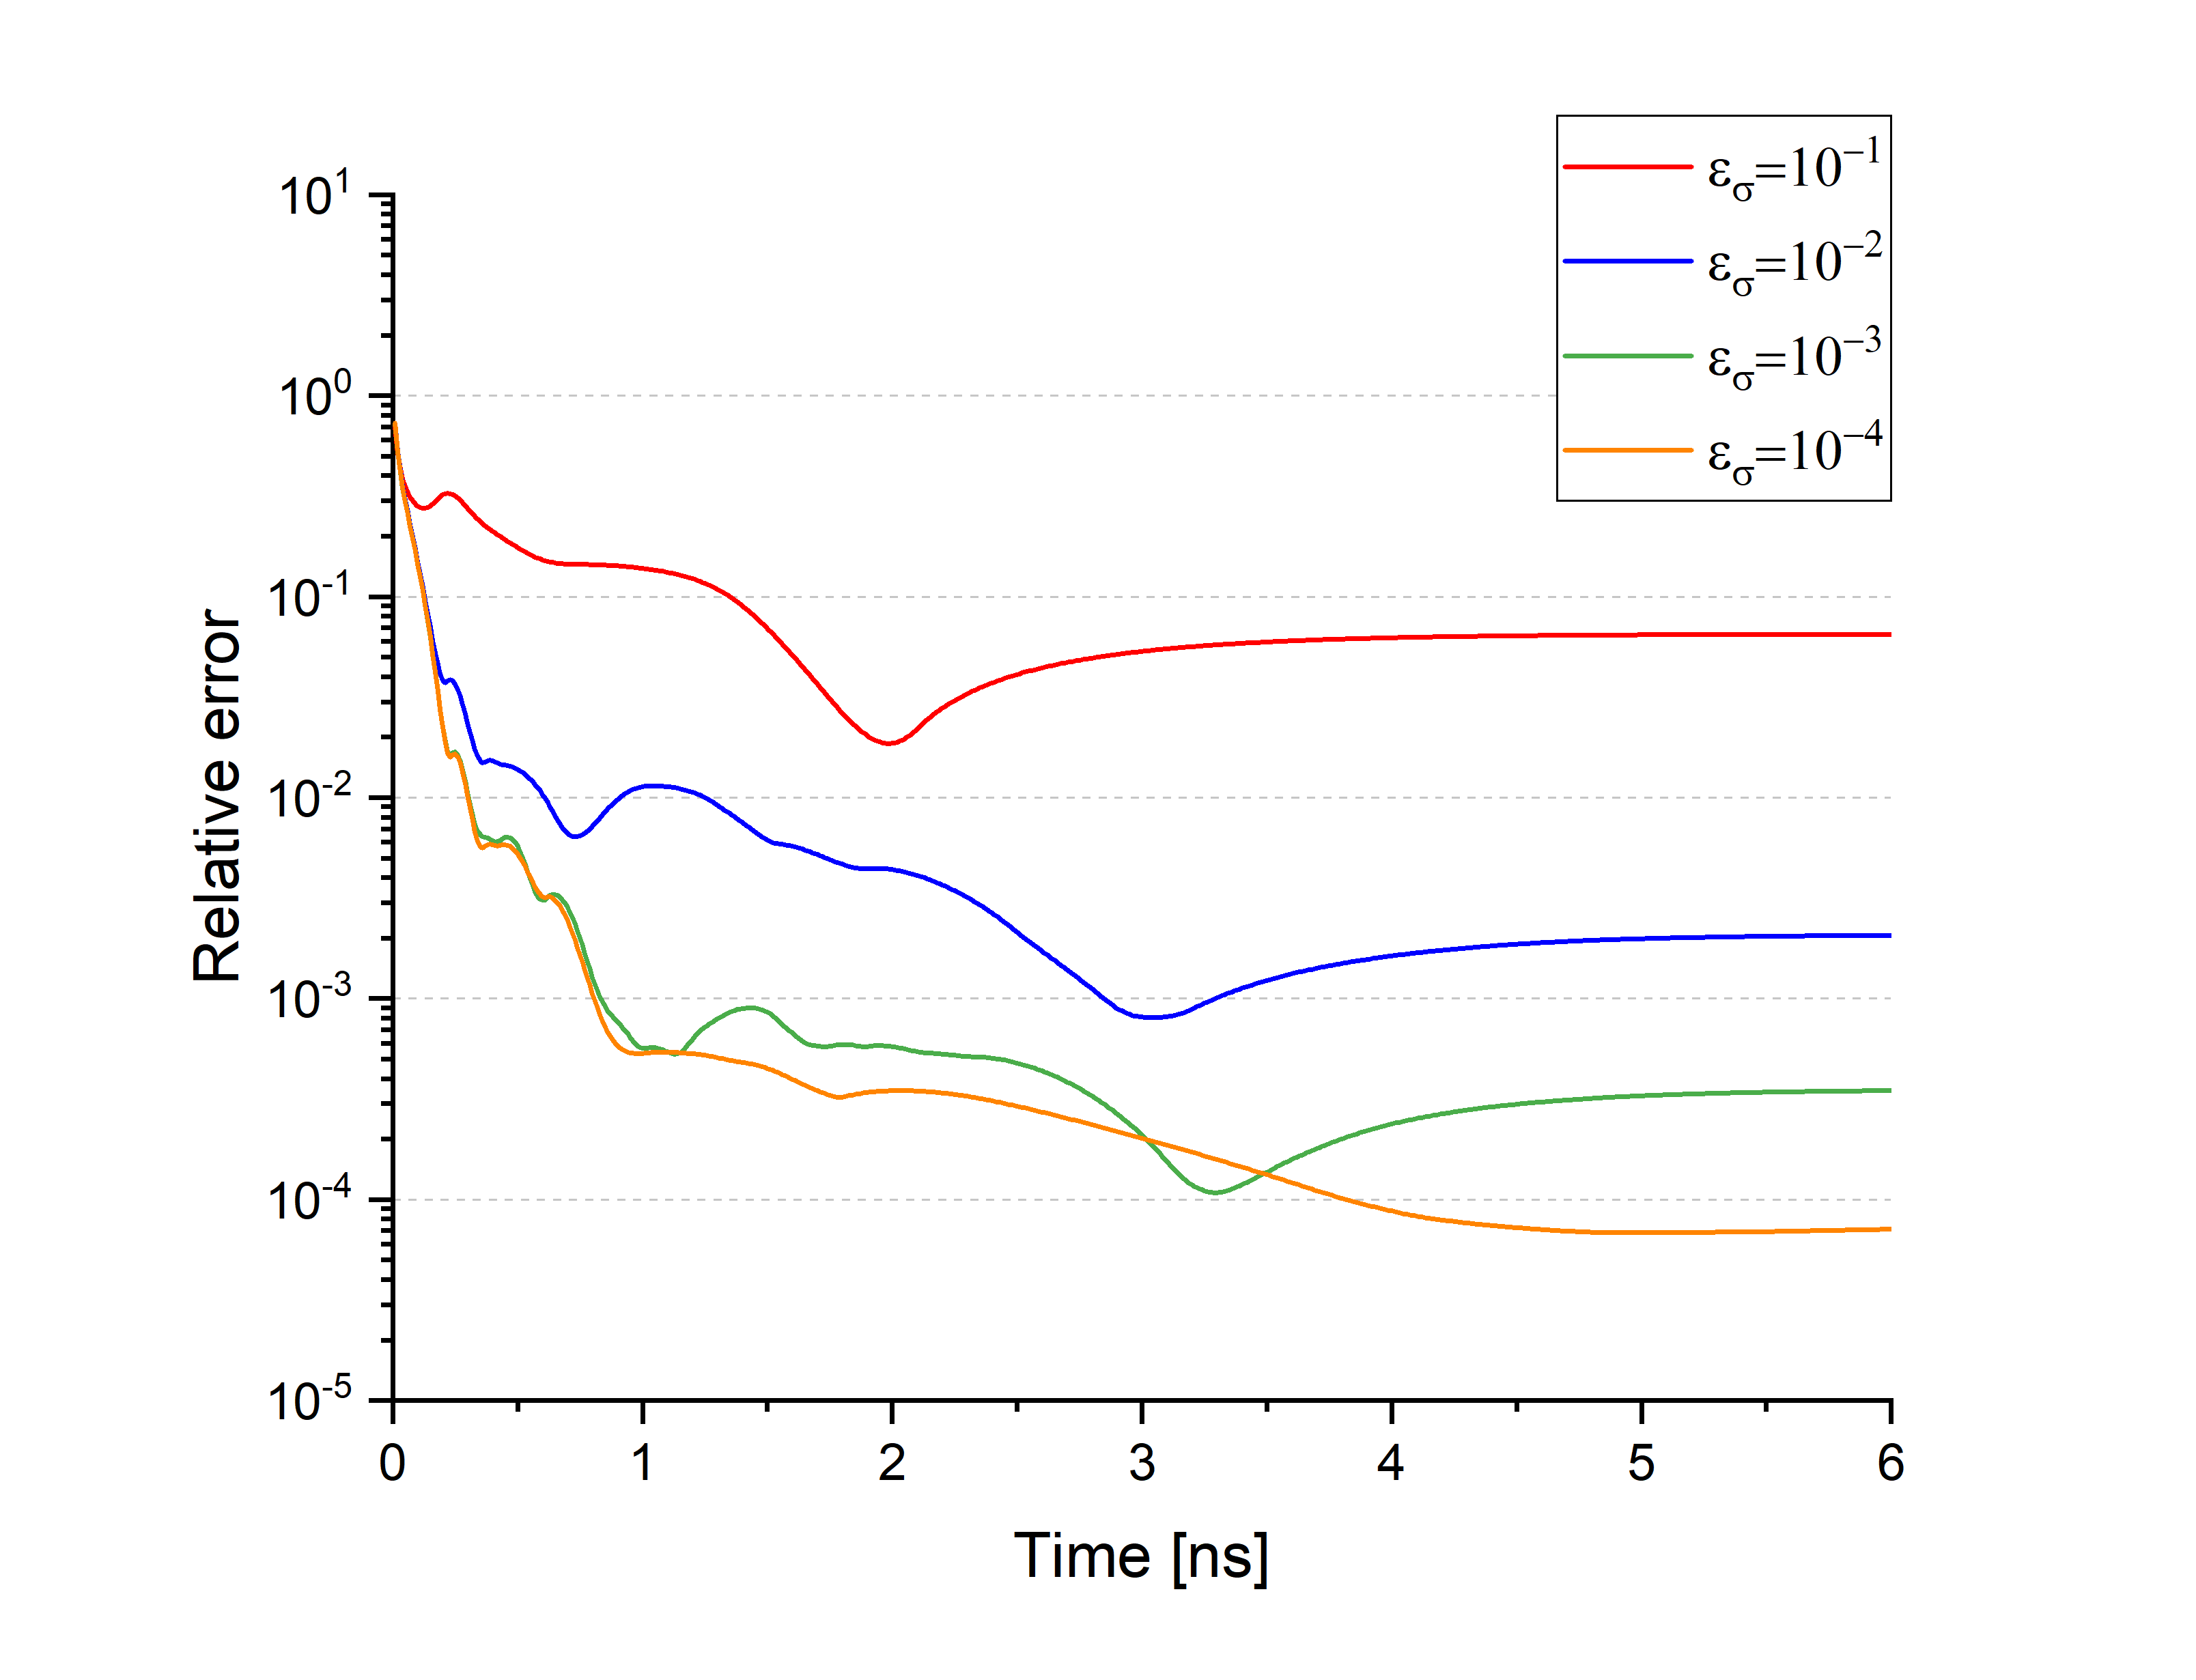
\includegraphics[width=0.5\textwidth]{MG_bc1000-t001_qdf1000-t002_Eavg_mlqd.png}}
		\caption{\label{fig:errors_dt-0.01}
			Relative error in the $L_1$-norm of MLOQD-POD ROM solutions  computed with $\Delta t\! =\! 1 \! \times \! 10^{-2}$~ns
			versus the reference TRT solution. The data for the MLOQD-POD ROM is generated with $\Delta t\! =\! 2 \! \times\!  10^{-2}$ ns. }
	\end{figure}

	\begin{figure}[ht!]
		\centering
		\subfloat[Temperature relative error \label{subfig-1:MG_bc1000-t0005_qdf1000-t002_Tavg_mlqd}]{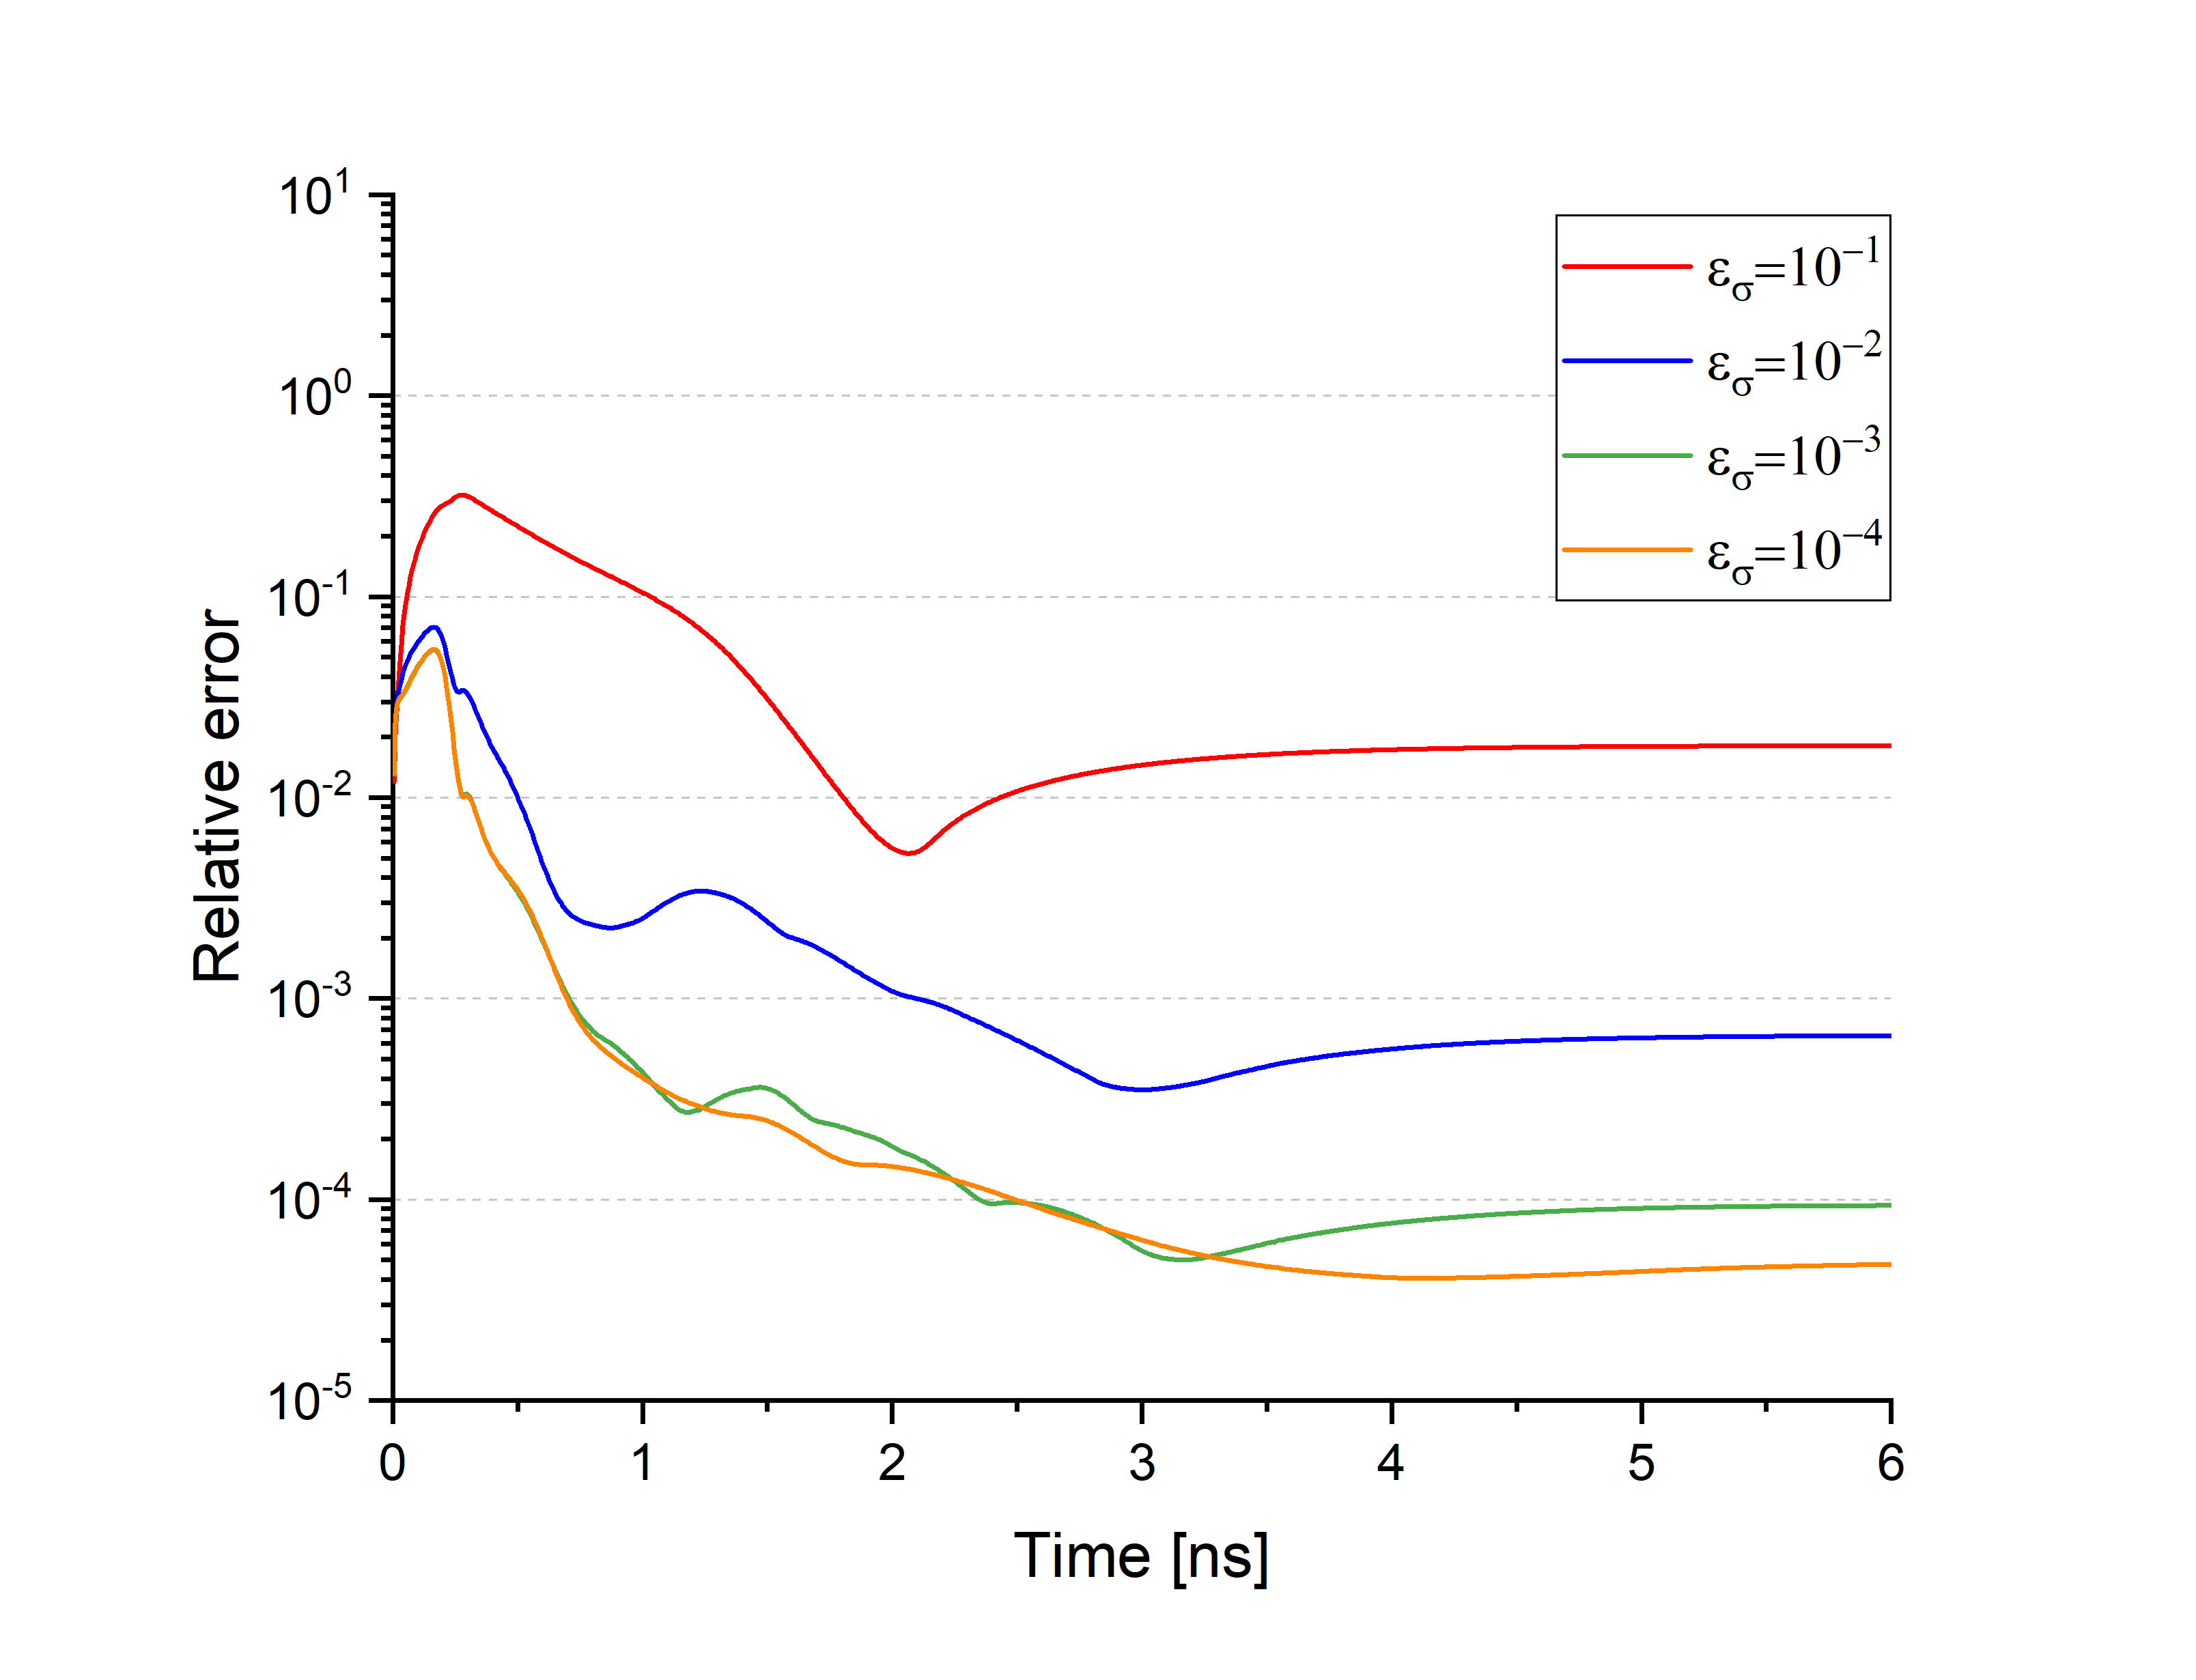
\includegraphics[width=0.5\textwidth]{MG_bc1000-t0005_qdf1000-t002_Tavg_mlqd.png}}
		\subfloat[Energy density relative error \label{subfig-1:MG_bc1000-t0005_qdf1000-t002_Eavg_mlqd}]{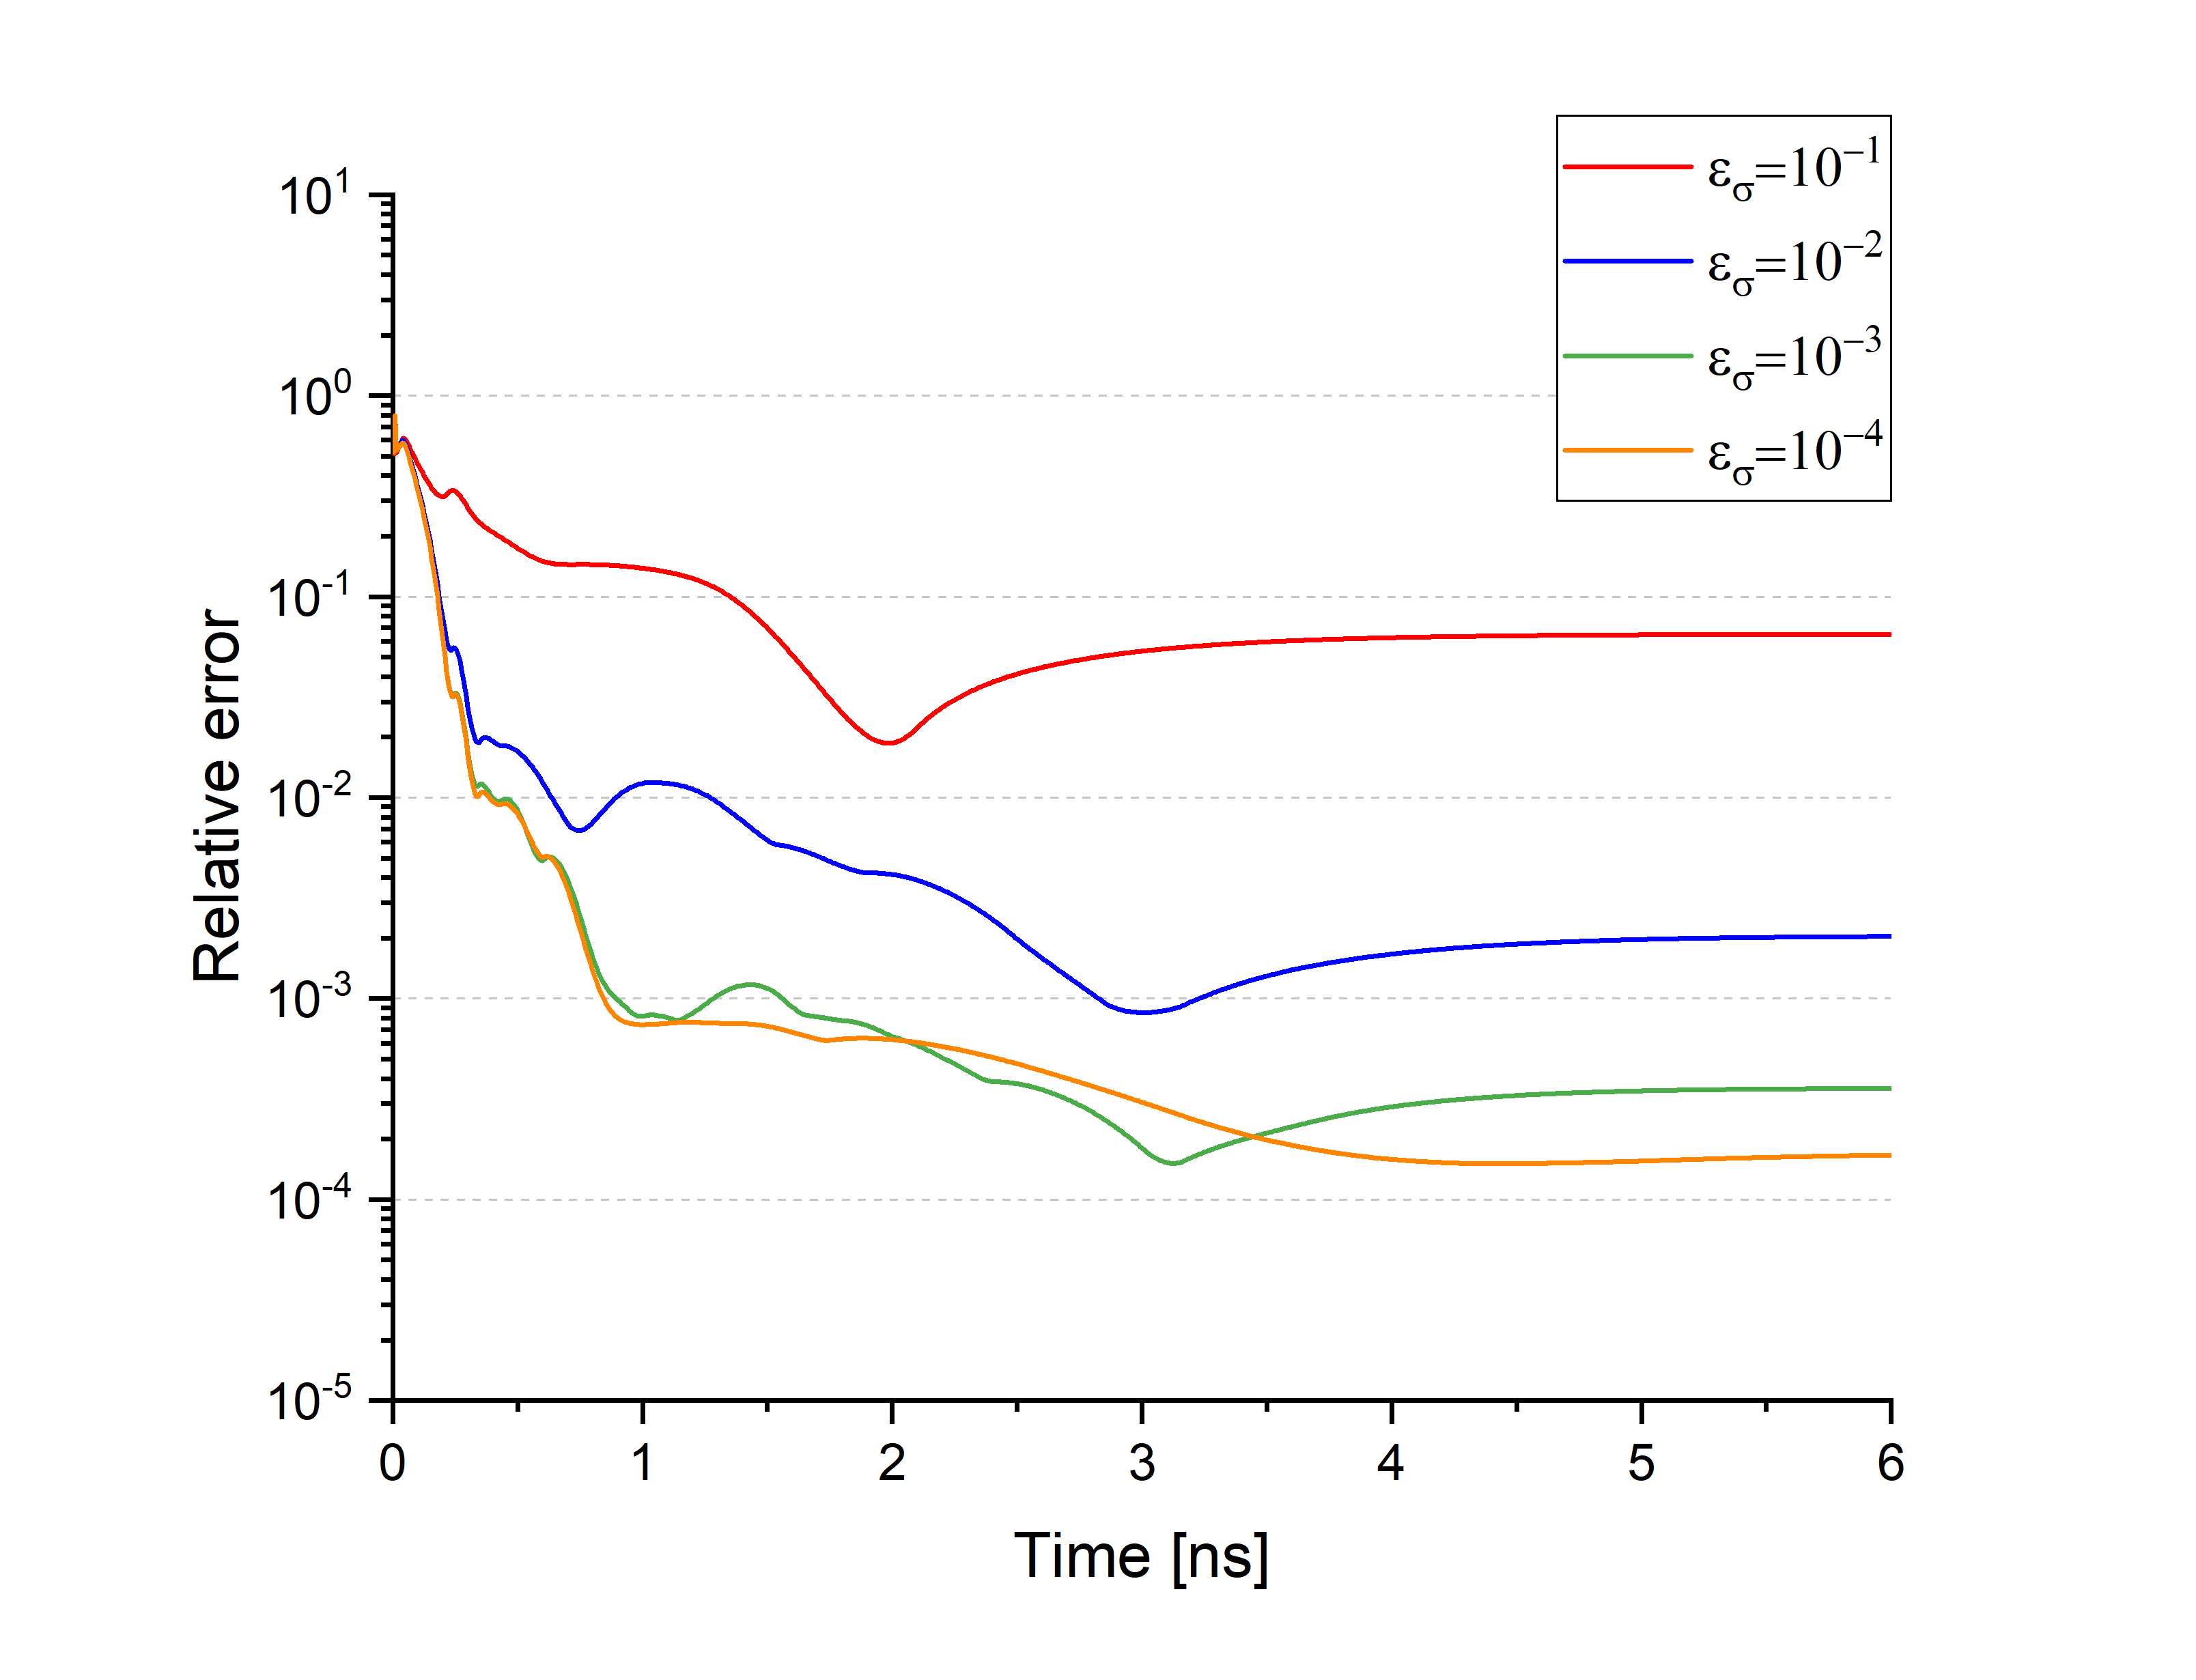
\includegraphics[width=0.5\textwidth]{MG_bc1000-t0005_qdf1000-t002_Eavg_mlqd.png}}
		\caption{\label{fig:errors_dt-0.005}
			Relative error in the $L_1$-norm of MLOQD-POD ROM solutions  computed with $\Delta t\! =\! 5 \! \times \! 10^{-3}$~ns
			versus the reference TRT solution. The data for the MLOQD-POD ROM is generated with $\Delta t\! =\! 2 \! \times\!  10^{-2}$ ns. }
	\end{figure}

	\begin{figure}[ht!]
		\centering
		\subfloat[Temperature relative error \label{subfig-1:MG_bc1000-t0002_qdf1000-t002_Tavg_mlqd}]{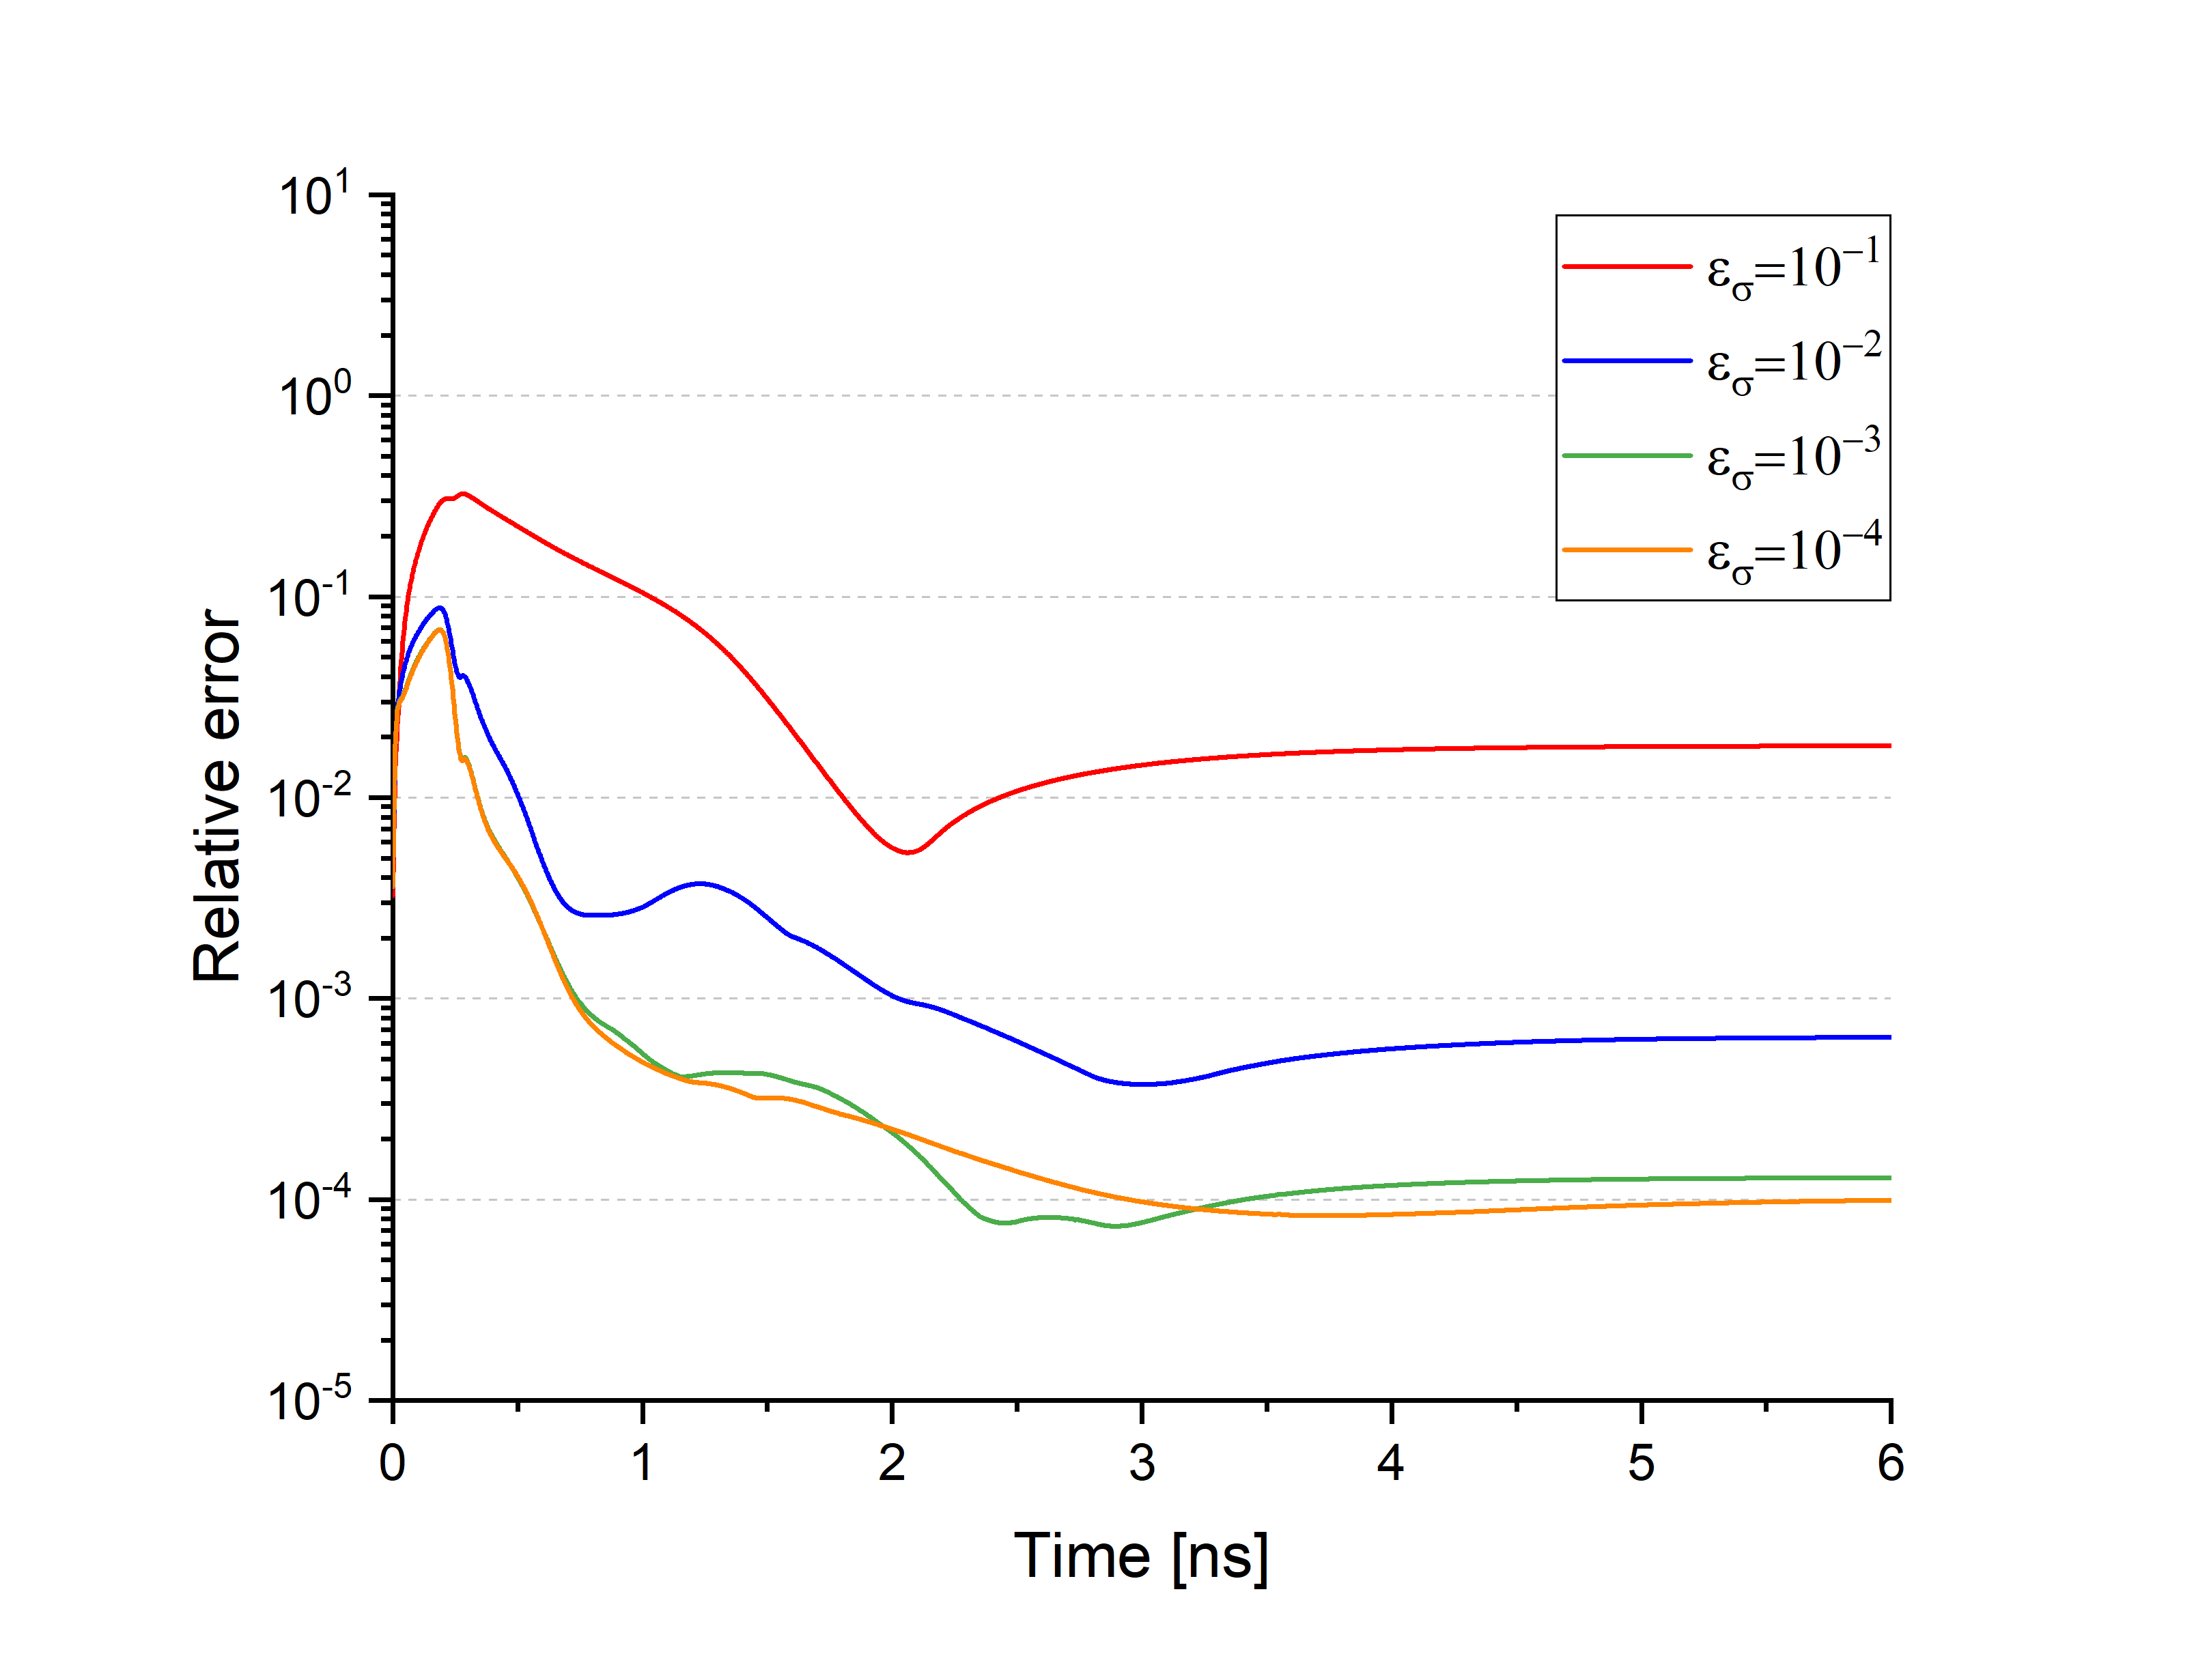
\includegraphics[width=0.5\textwidth]{MG_bc1000-t0002_qdf1000-t002_Tavg_mlqd.png}}
		\subfloat[Energy density relative error \label{subfig-1:MG_bc1000-t0002_qdf1000-t002_Eavg_mlqd}]{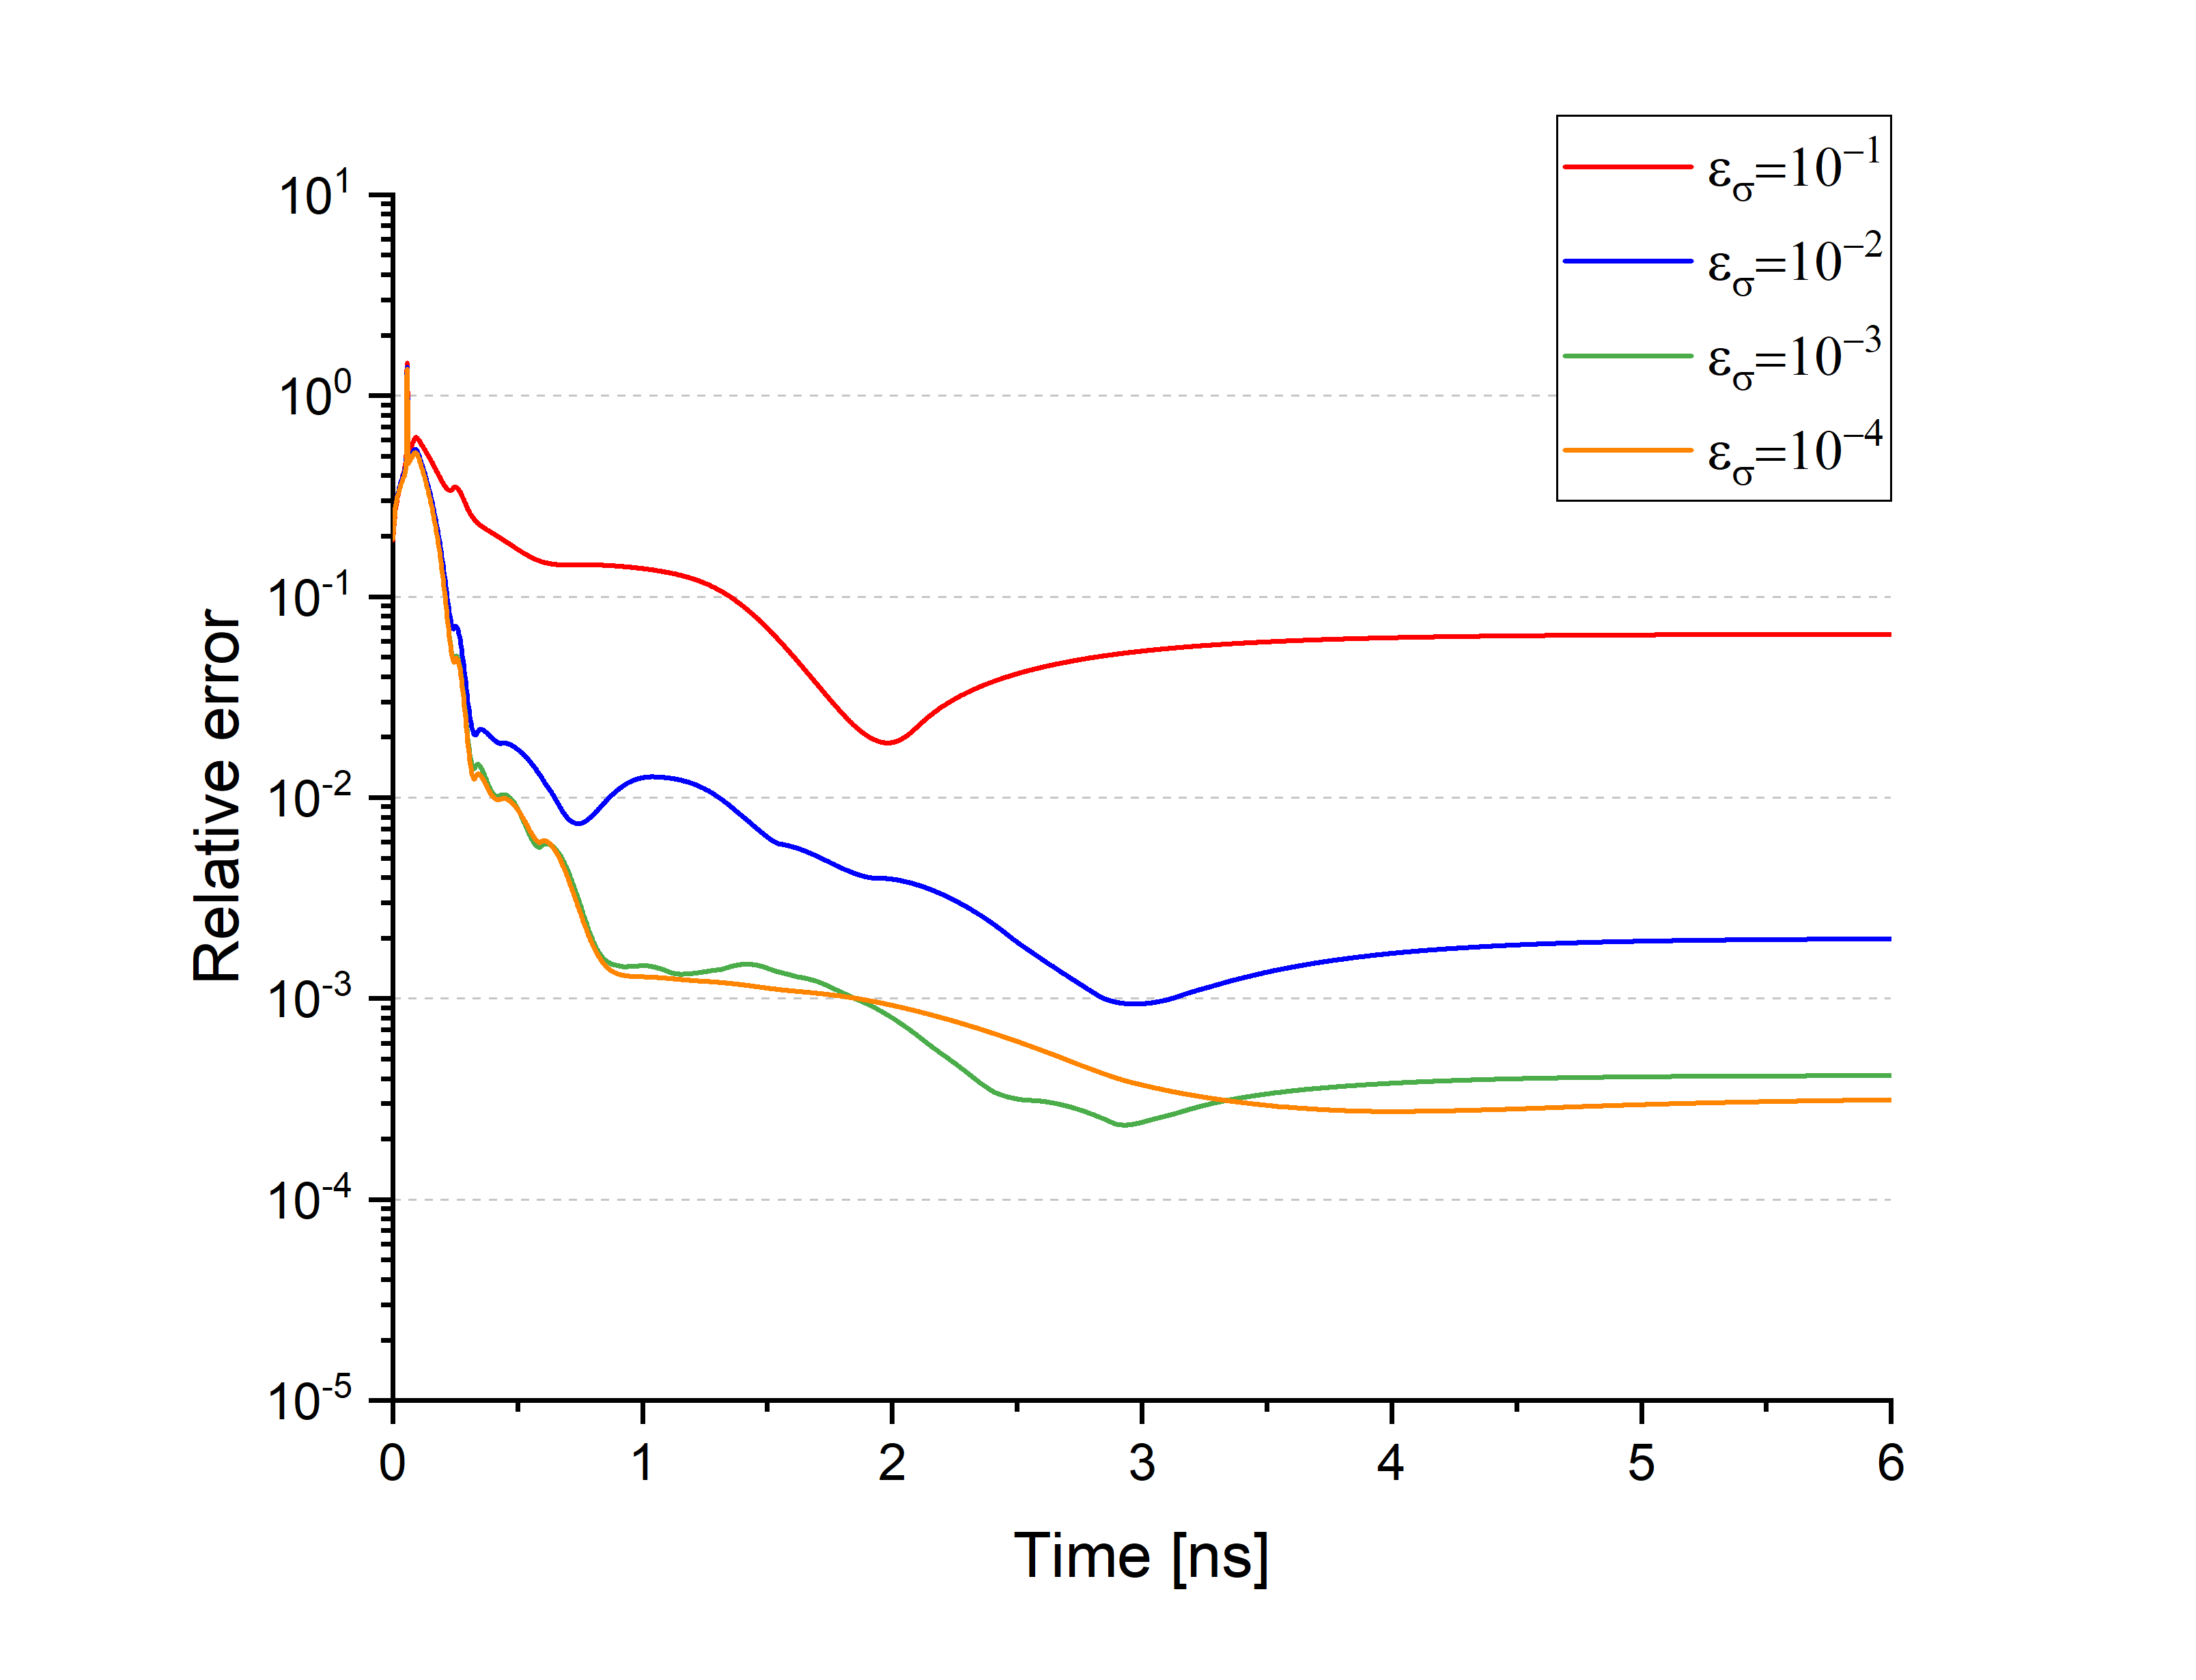
\includegraphics[width=0.5\textwidth]{MG_bc1000-t0002_qdf1000-t002_Eavg_mlqd.png}}
		\caption{\label{fig:errors_dt-0.002}
			Relative error in the $L_1$-norm of MLOQD-POD ROM solutions  computed with $\Delta t\! =\! 2 \! \times \! 10^{-3}$~ns
			versus the reference TRT solution. The data for the MLOQD-POD ROM is generated with $\Delta t\! =\! 2 \! \times\!  10^{-2}$ ns. }
	\end{figure}

	\ind The MLOQD-POD ROM can be further extended to develop a parameterized ROM for a class of TRT problems using QD factors estimated from a set of base cases. In this study we consider a ROM parameterized with respect to the temperature $T_{in}$ of incoming radiation at the left boundary. A database of the group QD factors for problems with two selected temperatures of incoming radiation  $T_{in}^{(1)}$ and $T_{in}^{(2)}$ is constructed. The MLOQD-POD ROM solutions of TRT problems with incoming radiation at some given temperature are calculated using group QD factors obtained by linear interpolation between values in the database. Results are presented for three parameterized ROMs. One model uses $T_{in}^{(1)}~=~1$~KeV and $T_{in}^{(2)}=0.98$ KeV. The second model is formed with  $T_{in}^{(1)}=1$ KeV and $T_{in}^{(2)}=0.96$ KeV. The third is formed with  $T_{in}^{(1)}=1$ KeV and $T_{in}^{(2)}=0.92$ KeV. The databases are generated for $\Delta t = 2\times10^{-2}$ ns. Figure \ref{fig:errors_bc_T=990} shows  the  relative error in $L_1$-norm in the solution  for $T_{in}=0.99$ KeV computed by means of first parameterized MLOQD-POD ROM with various values of $\varepsilon_{\sigma}$. Figure \ref{fig:errors_bc_T=980} presents the relative error of the MLOQD-POD ROM solution  for $T_{in}= 0.98$ KeV obtained from the second model that is parameterized with a larger interval of  $[T_{in}^{(1)},T_{in}^{(2)}]$. Figure \ref{fig:errors_bc_T=960} presents the relative error of the MLOQD-POD ROM solution  for $T_{in}= 0.96$ KeV obtained from the third model that is parameterized with the largest interval of  $[T_{in}^{(1)},T_{in}^{(2)}]$. The reference solution is computed for each value of $T_{in}$ to obtain relative errors. The error in the MLOQD-POD ROM saturates at $\varepsilon_\sigma=10^{-6}$ and smaller values are not shown. Compared to the ROMs that used a reduced time step length compared to the database, the error displayed here is more uniform across time, and the lowest error found is smaller. As the interval $[T_{in}^{(1)},T_{in}^{(2)}]$ increases the error at $\varepsilon_\sigma=10^{-6}$ increases. However, the error associated with $\varepsilon_\sigma=10^{-1}$ does not visibly change on the plots shown.
	
	%=================================================================================
	% BOUNDARY CONDITION DATABASE ERRORS PLOT
	\begin{figure}[ht!]
		\centering
		\subfloat[Temperature relative error \label{subfig:MG_bc990-t002_qdf1000-980-t002_Tavg_mlqd}]{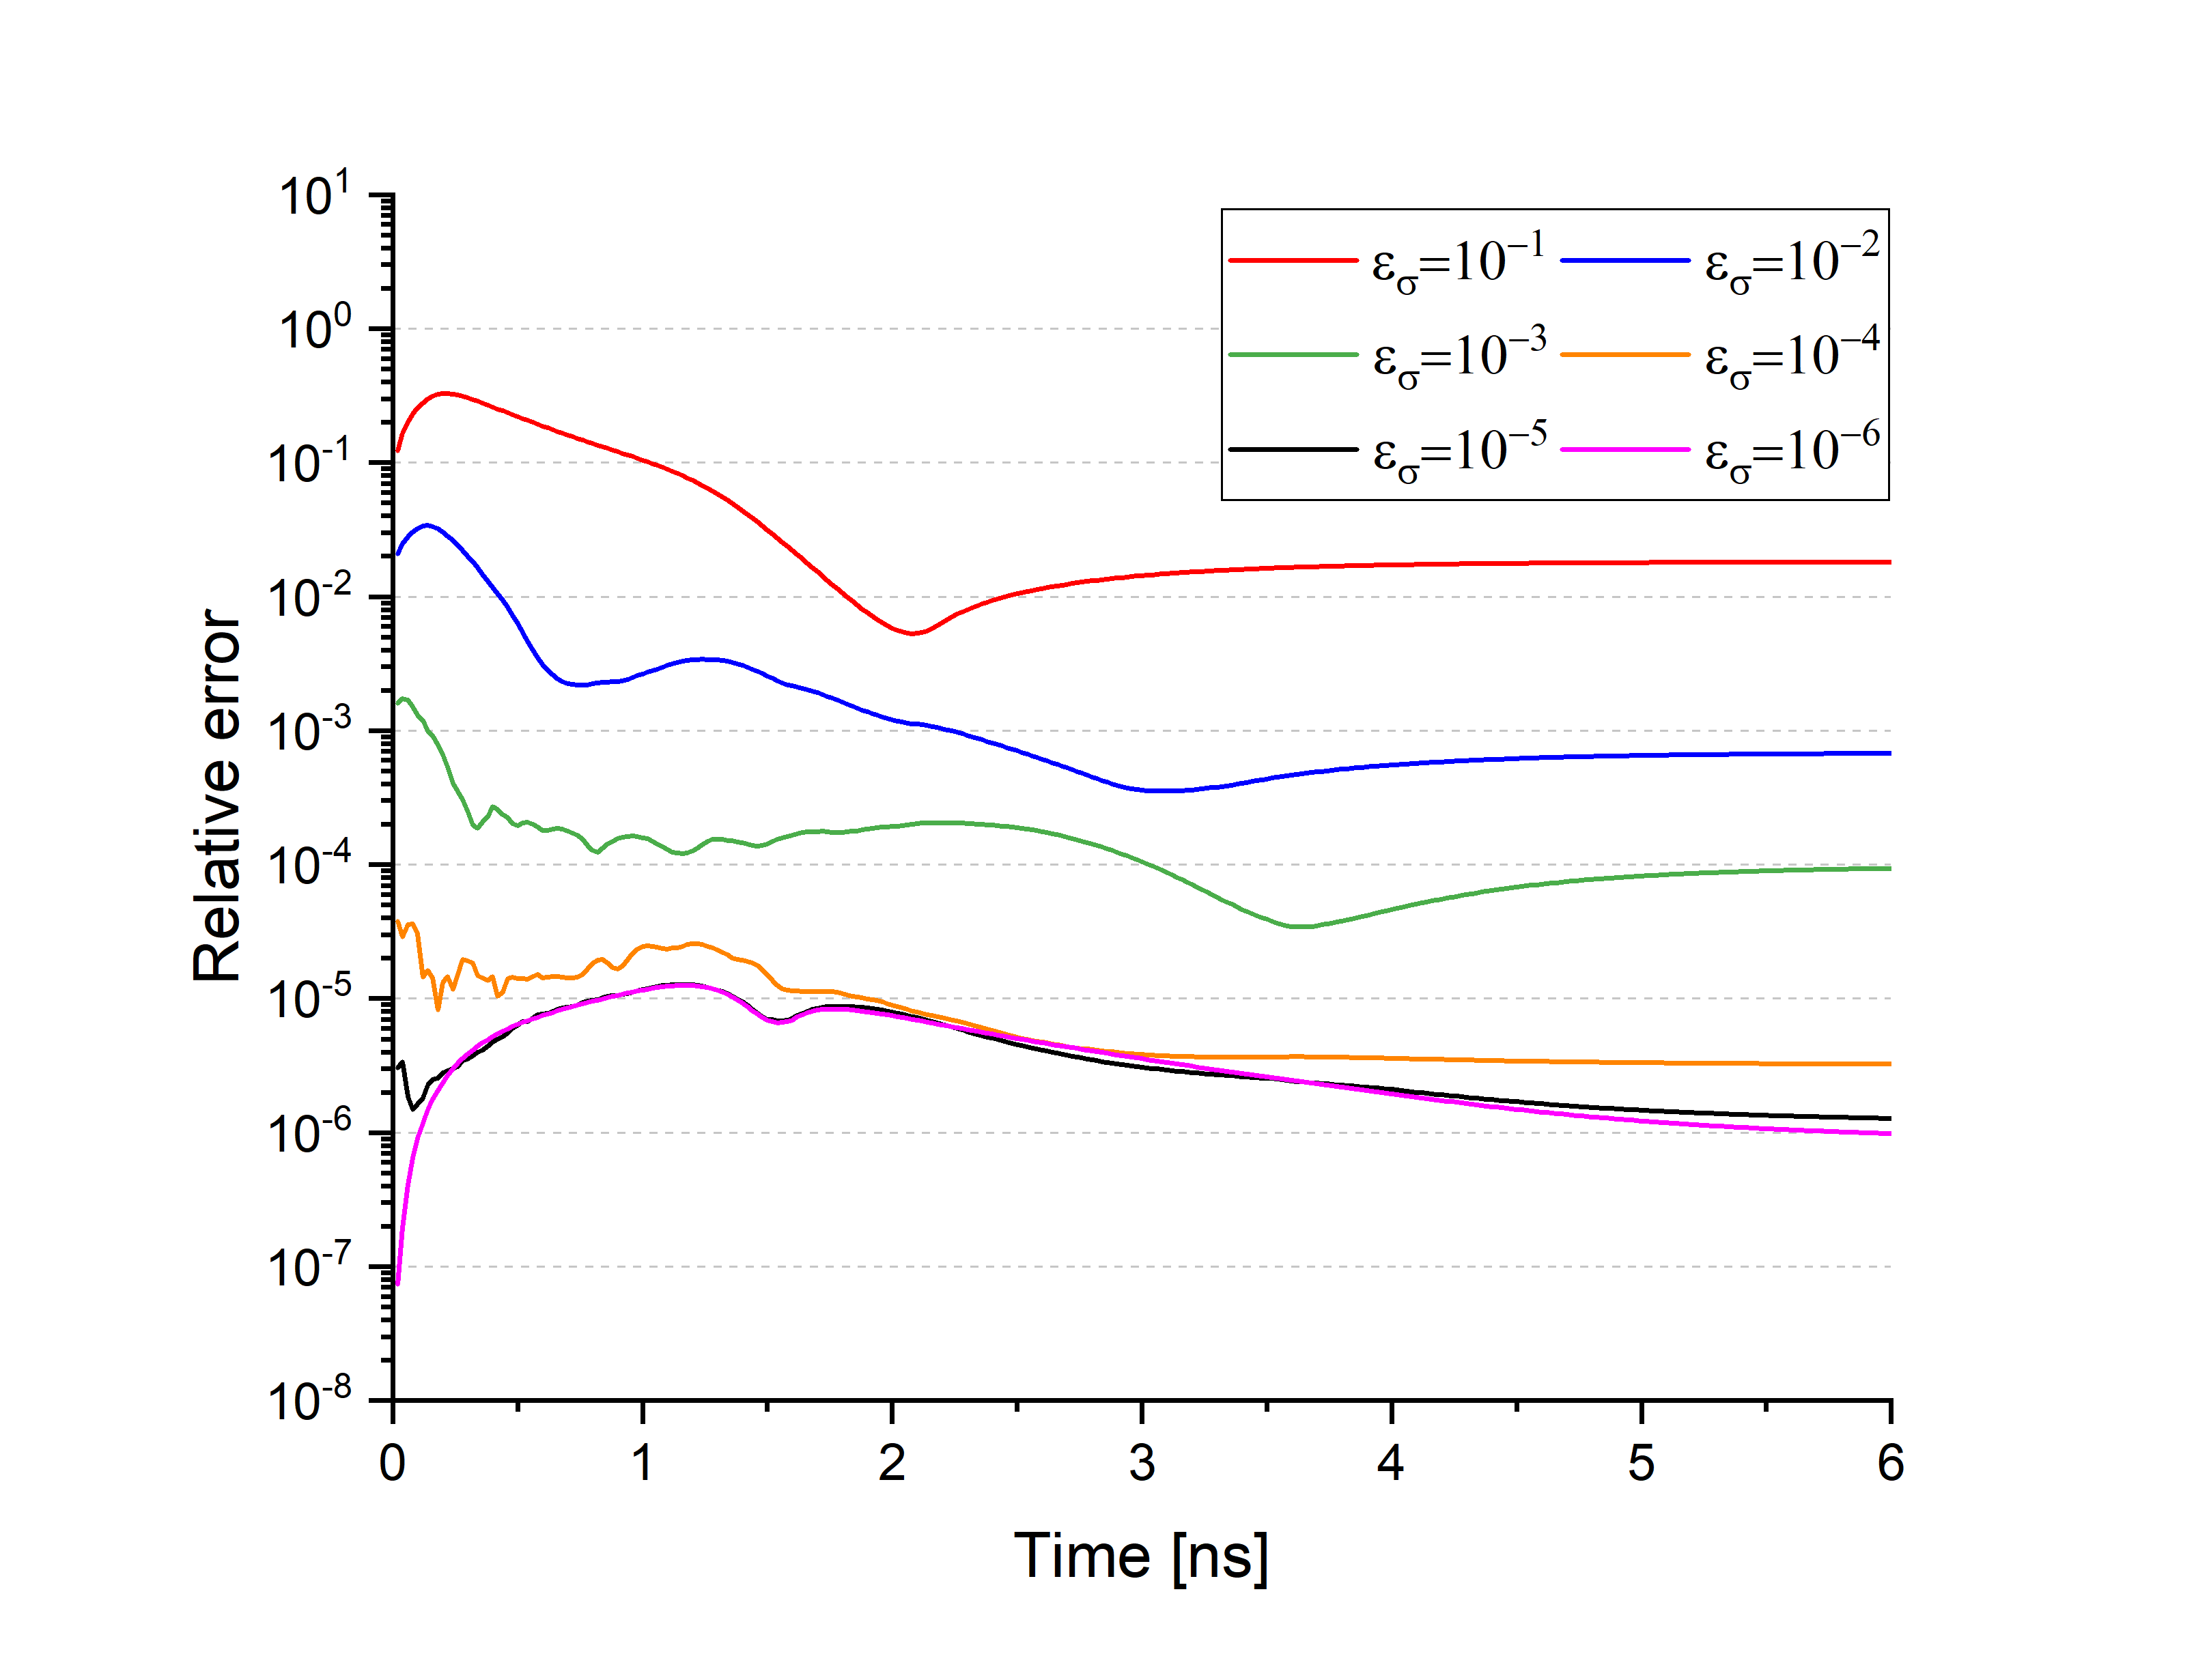
\includegraphics[width=0.5\textwidth]{MG_bc990-t002_qdf1000-980-t002_Tavg_mlqd.png}}
		\subfloat[Energy density relative error \label{subfig:MG_bc990-t002_qdf1000-980-t002_Eavg_mlqd}]{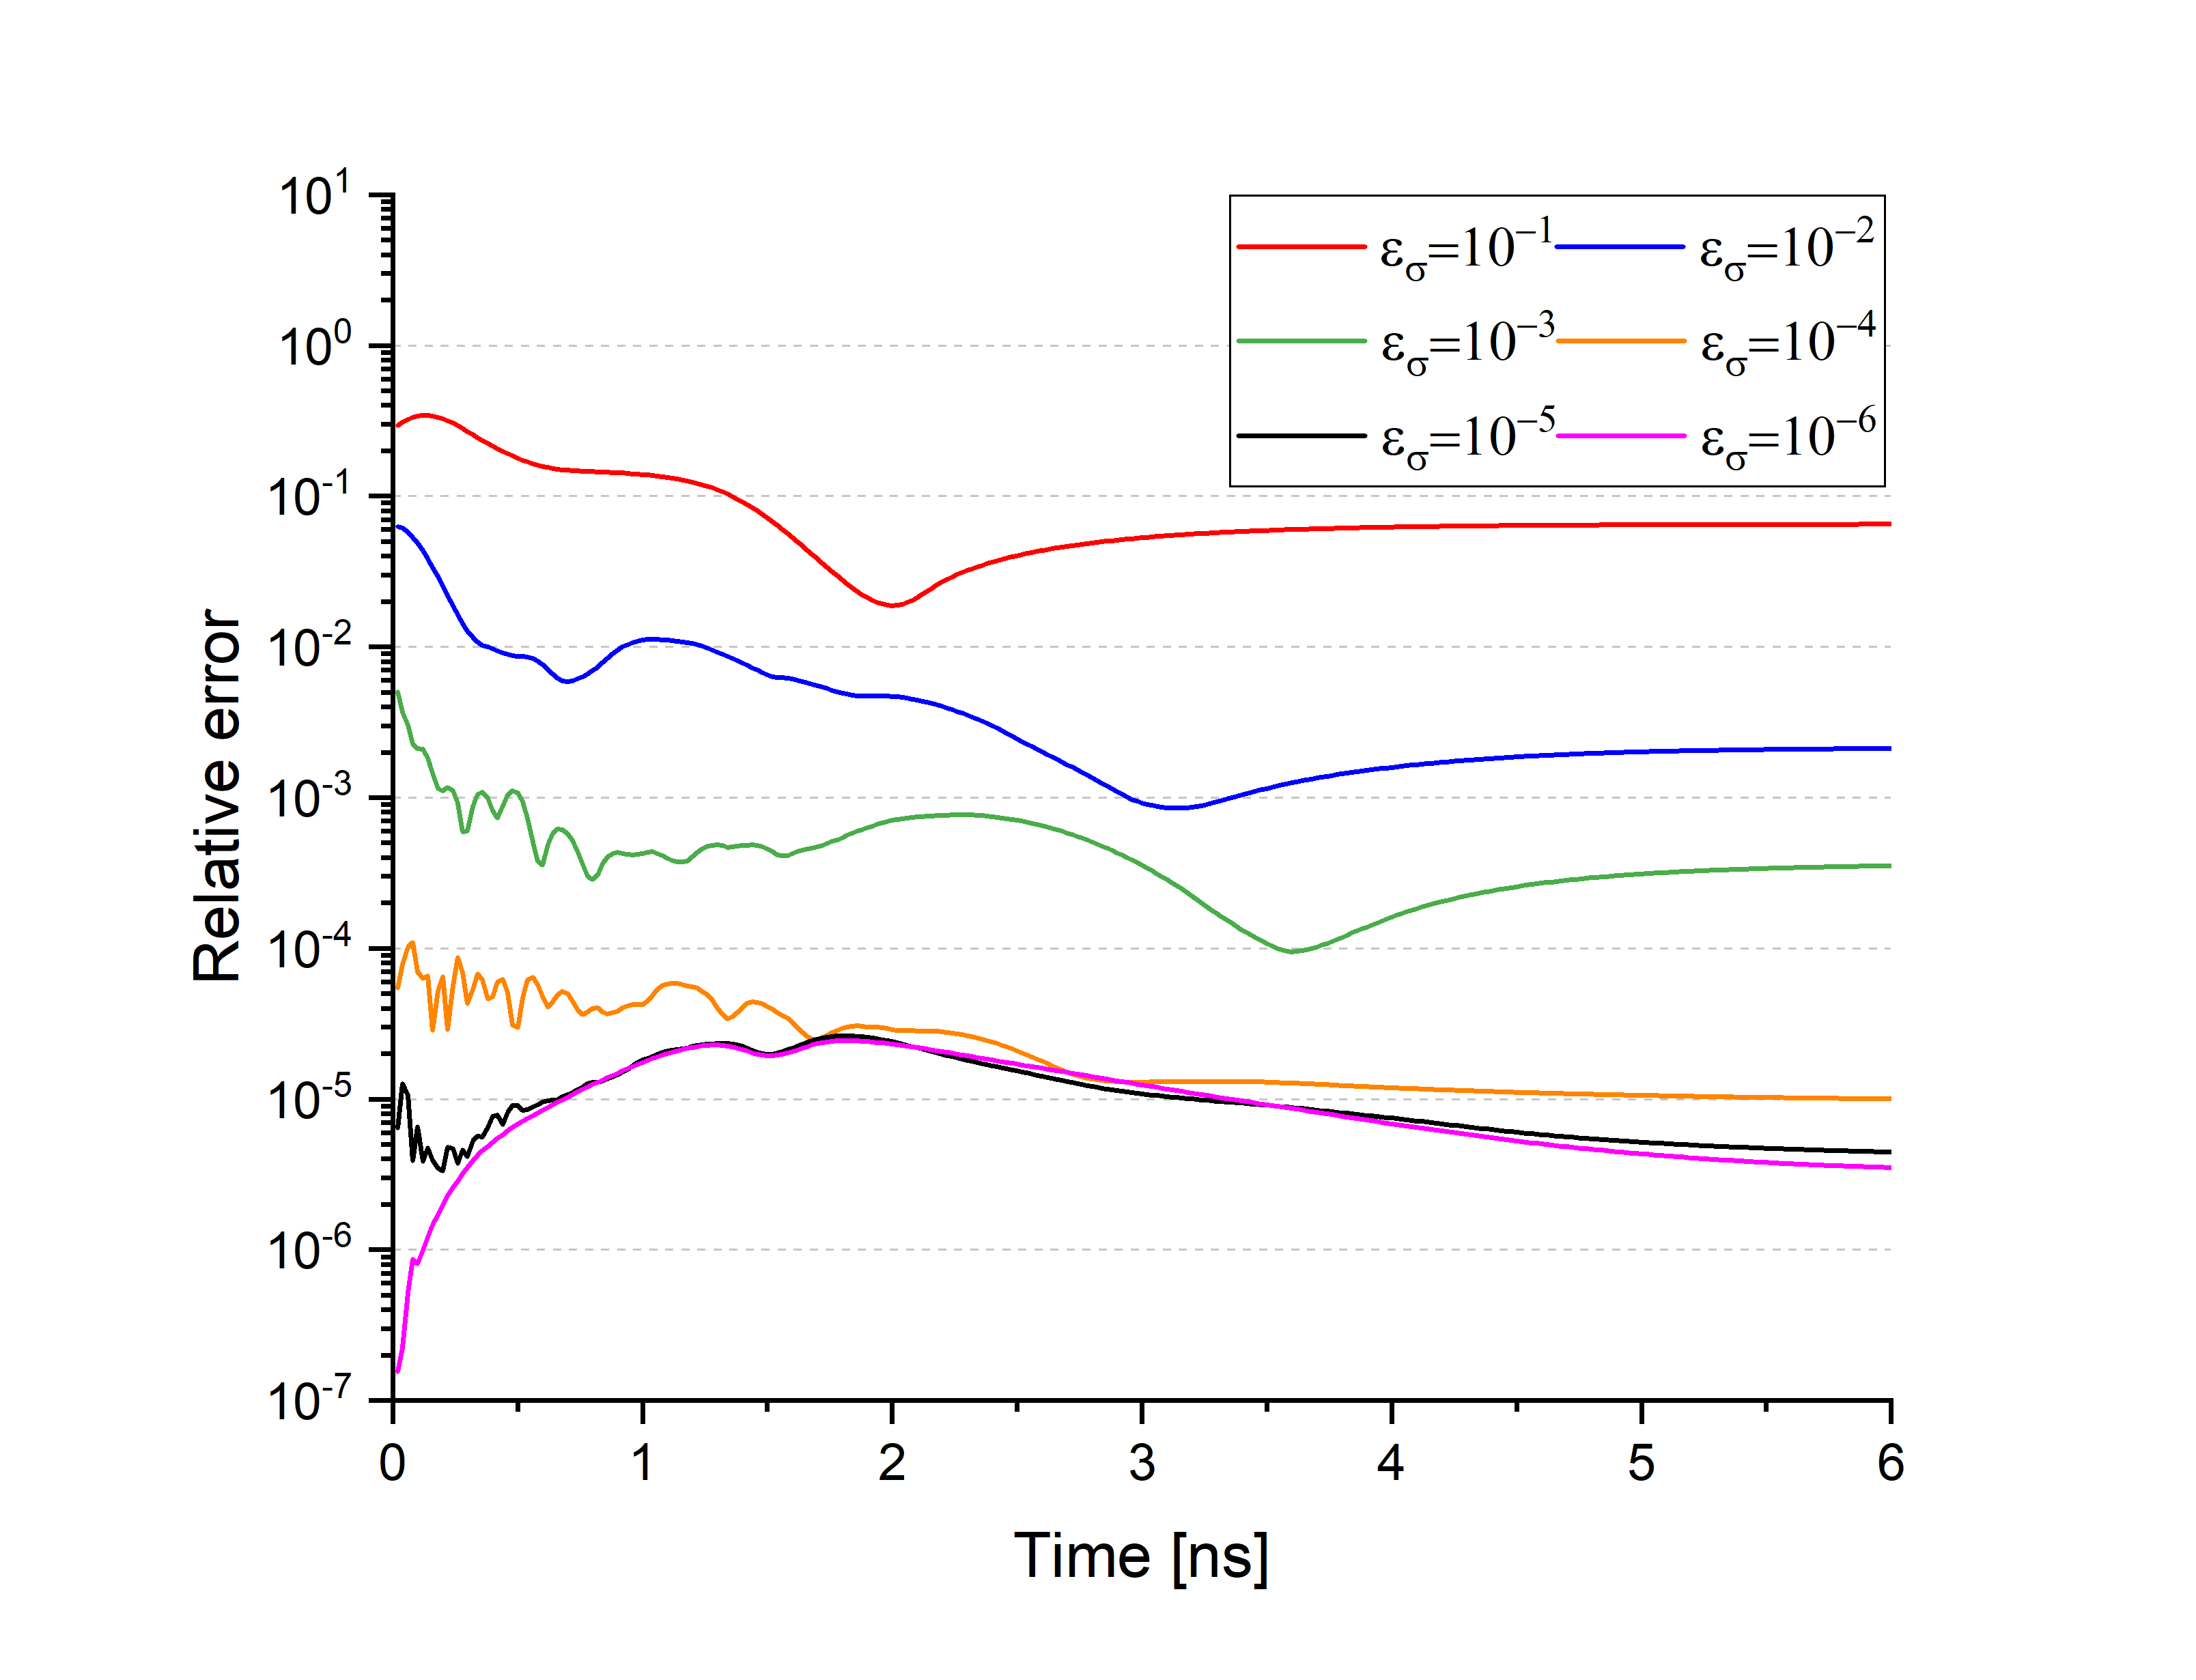
\includegraphics[width=0.5\textwidth]{MG_bc990-t002_qdf1000-980-t002_Eavg_mlqd.png}}
		\caption{\label{fig:errors_bc_T=990}
			Relative error in the $L_1$-norm of the MLOQD-POD ROM solutions computed with $T_{in}~=~0.99$~KeV using base cases with $T_{in}^{\pr{1}}=1$ KeV  and $T_{in}^{\pr{2}}=0.98$ KeV. }
	\end{figure}

	\begin{figure}[ht!]
		\centering
		\subfloat[Temperature relative error \label{subfig:MG_bc980-t002_qdf1000-960-t002_Tavg_mlqd}]{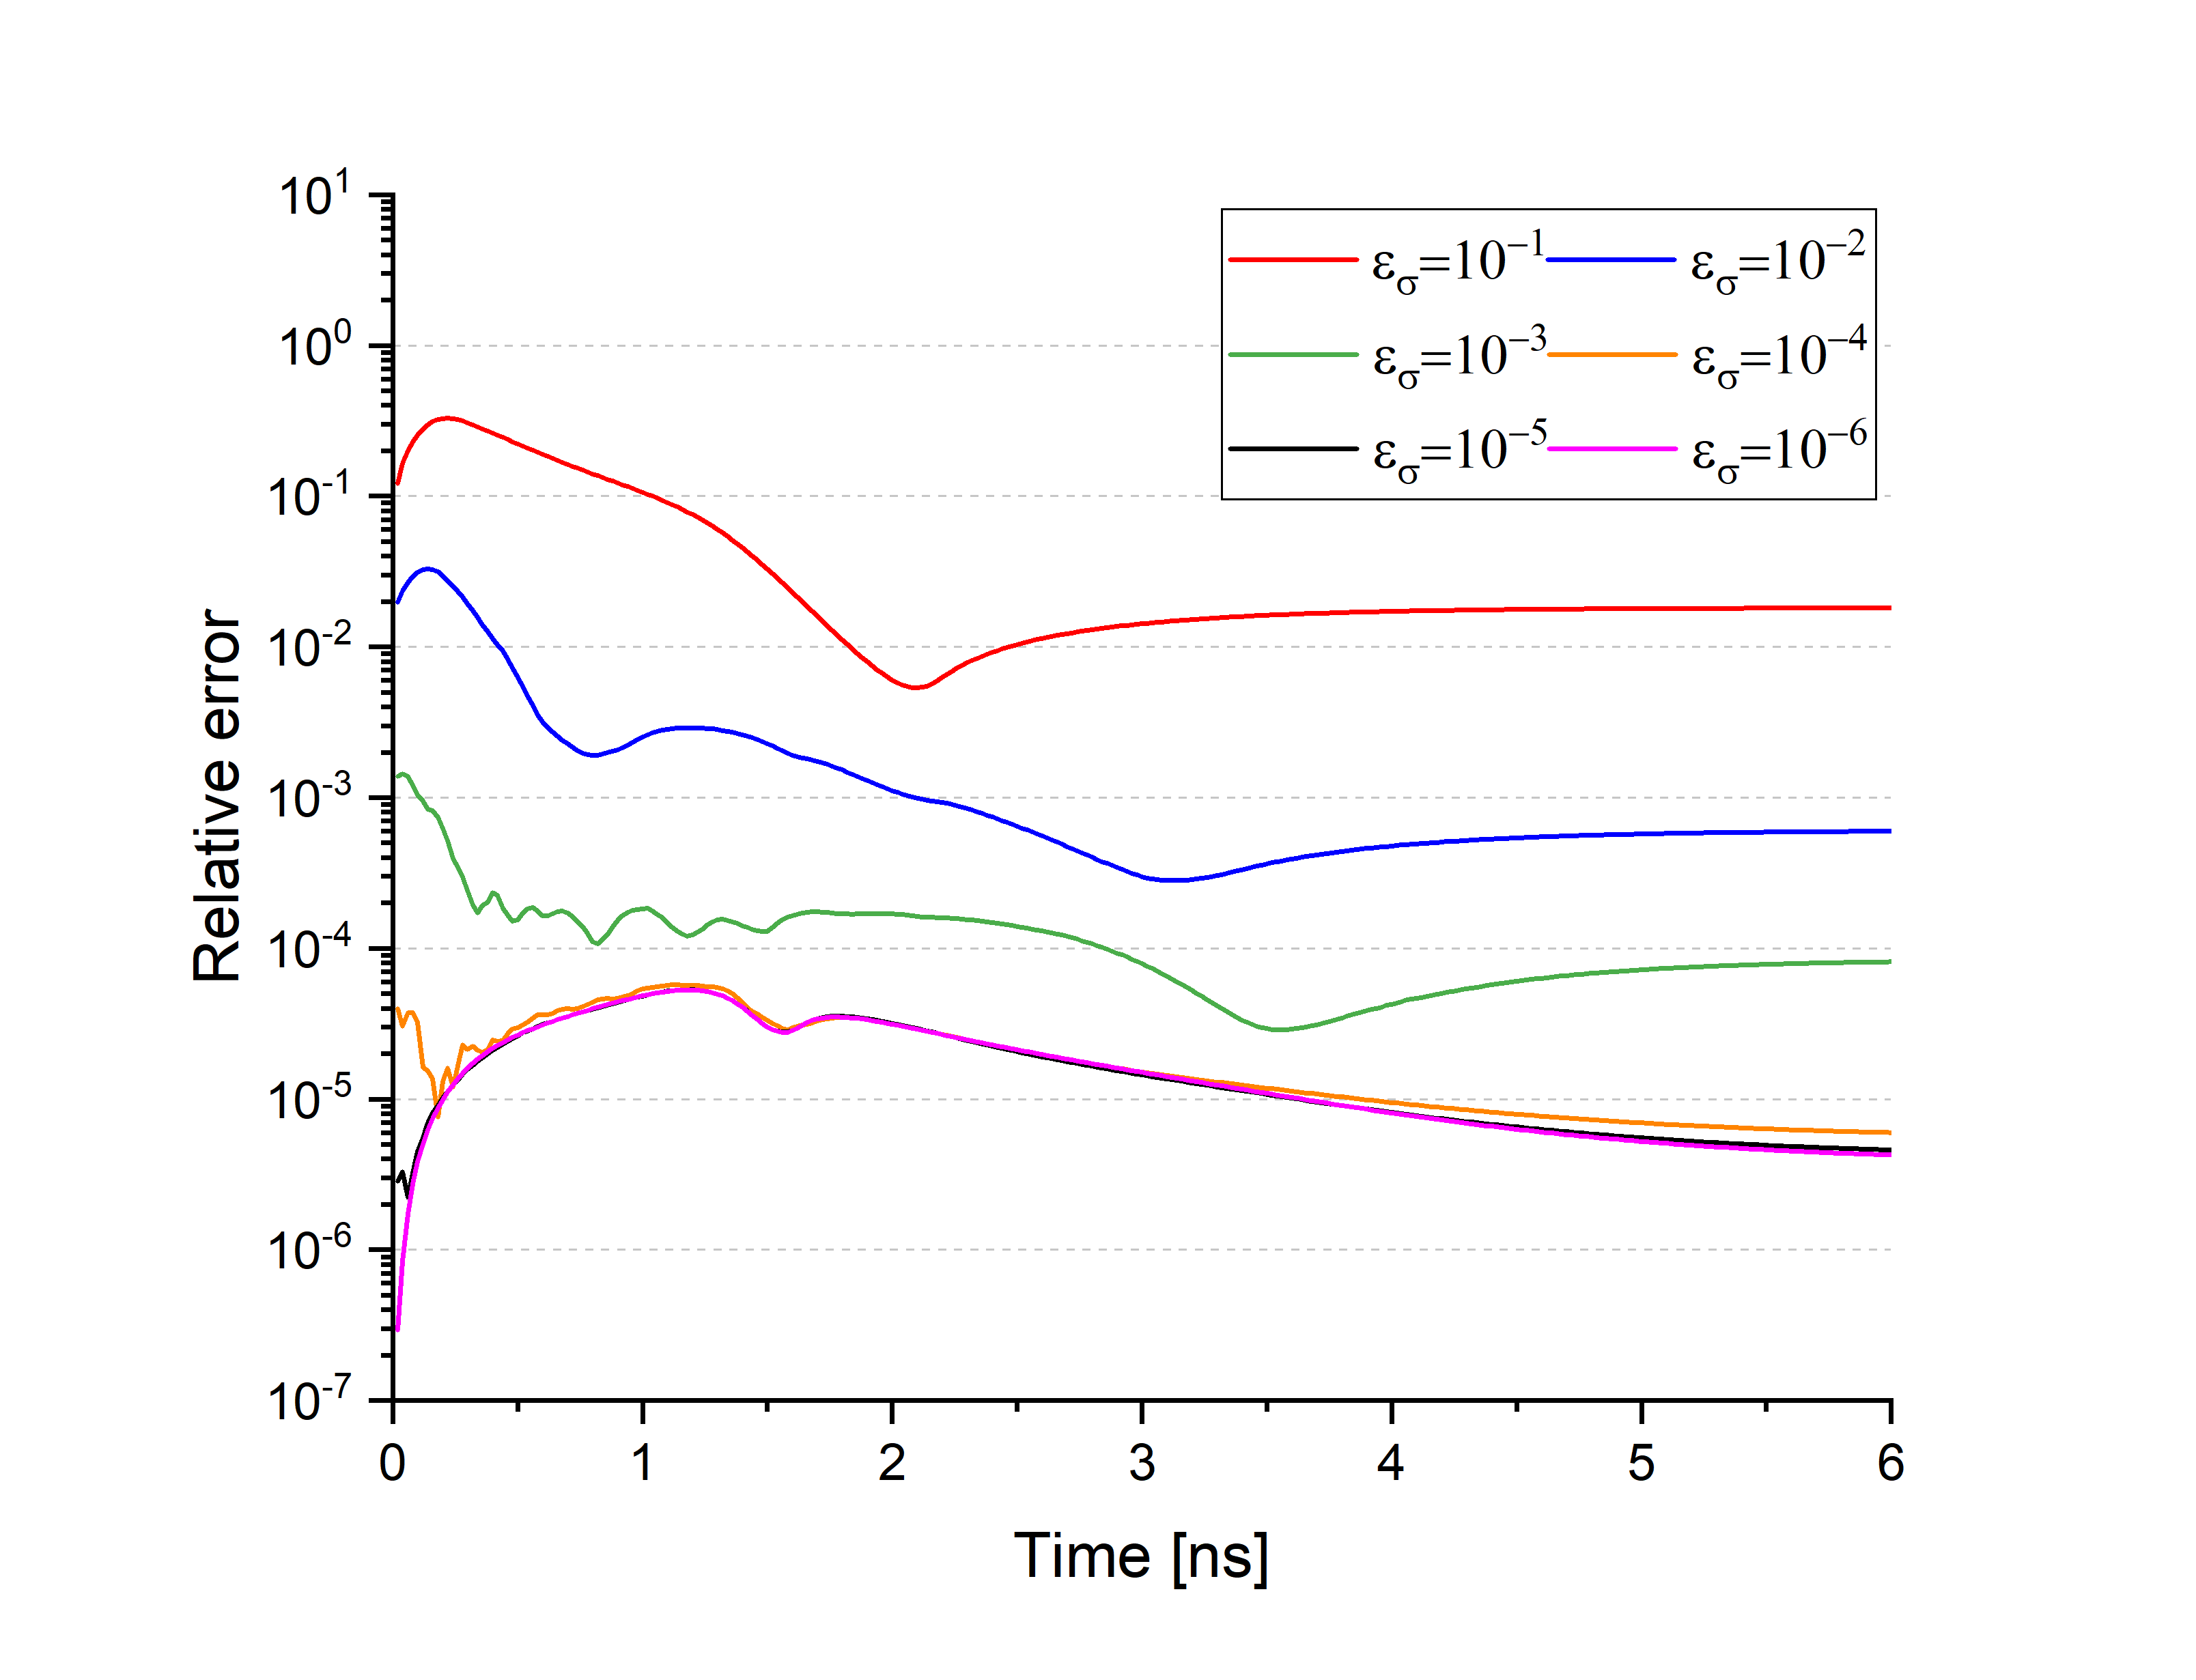
\includegraphics[width=0.5\textwidth]{MG_bc980-t002_qdf1000-960-t002_Tavg_mlqd.png}}
		\subfloat[Energy density relative error \label{subfig:MG_bc980-t002_qdf1000-960-t002_Eavg_mlqd}]{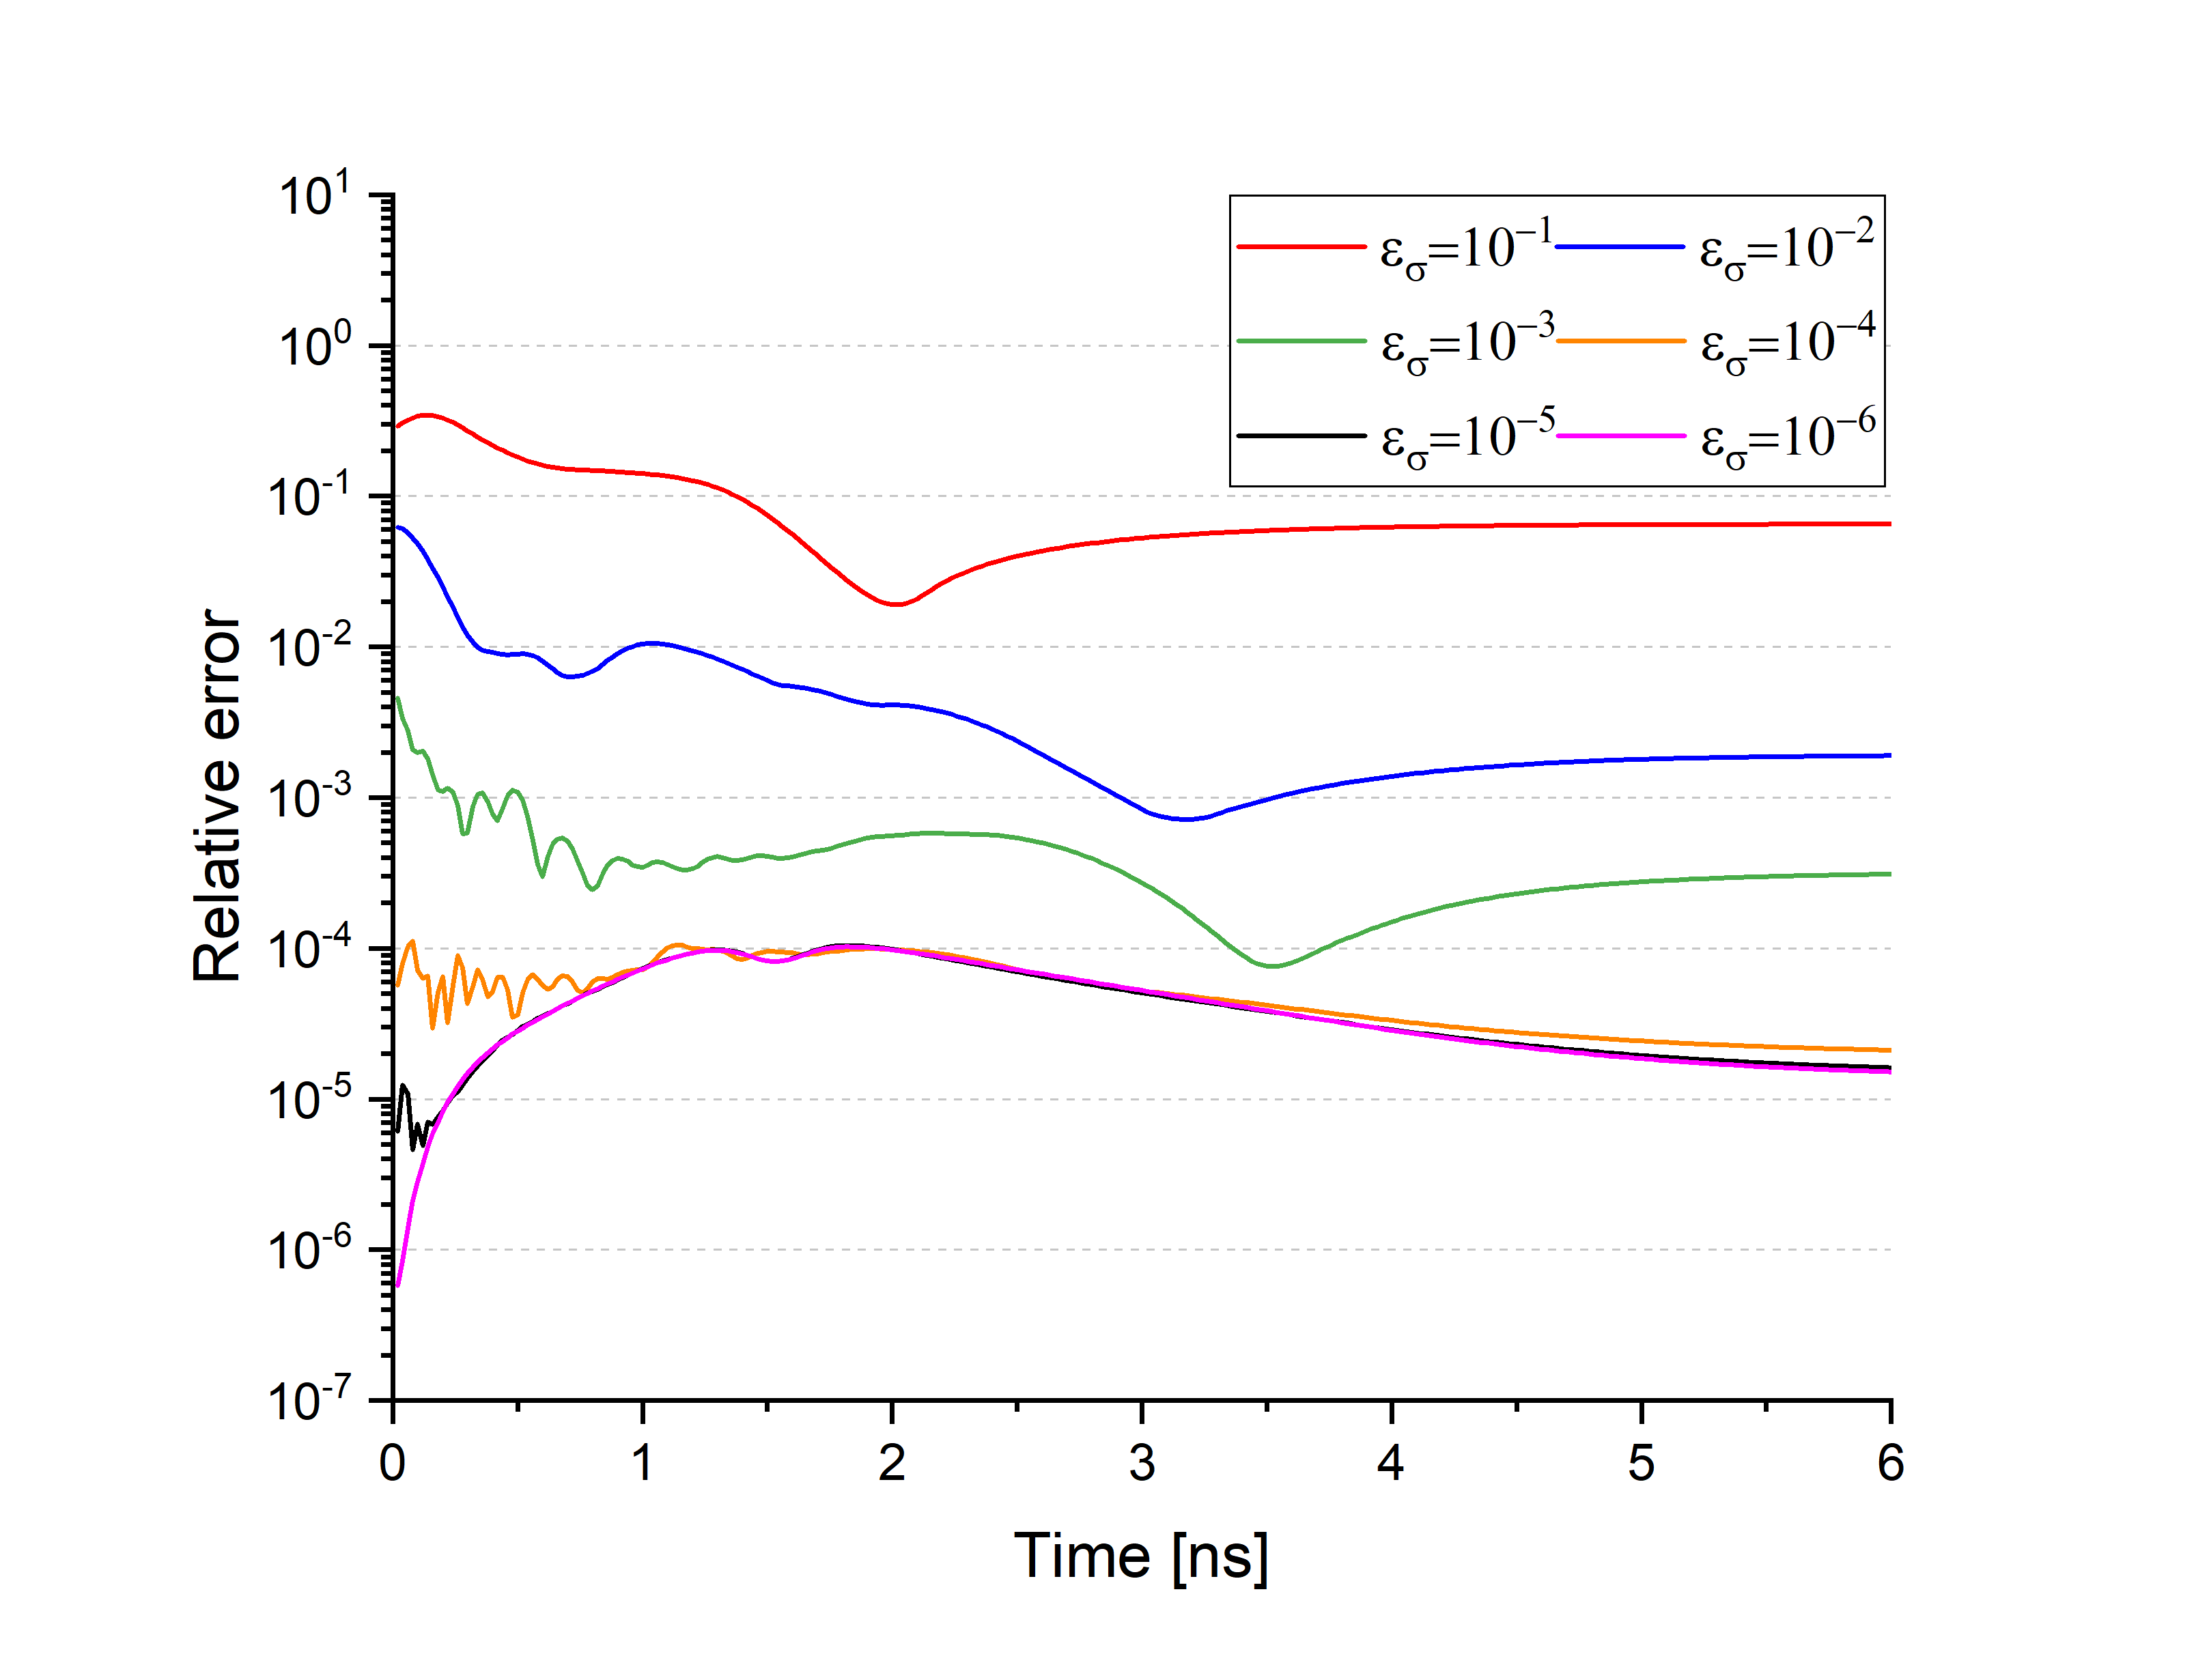
\includegraphics[width=0.5\textwidth]{MG_bc980-t002_qdf1000-960-t002_Eavg_mlqd.png}}
		\caption{\label{fig:errors_bc_T=980}
			Relative error in the $L_1$-norm of the MLOQD-POD ROM solutions computed with $T_{in}~=~0.98$~KeV using base cases with $T_{in}^{\pr{1}}=1$ KeV  and $T_{in}^{\pr{2}}=0.96$ KeV.}
	\end{figure}

	\begin{figure}[ht!]
		\centering
		\subfloat[Temperature relative error \label{subfig:MG_bc960-t002_qdf1000-920-t002_Tavg_mlqd}]{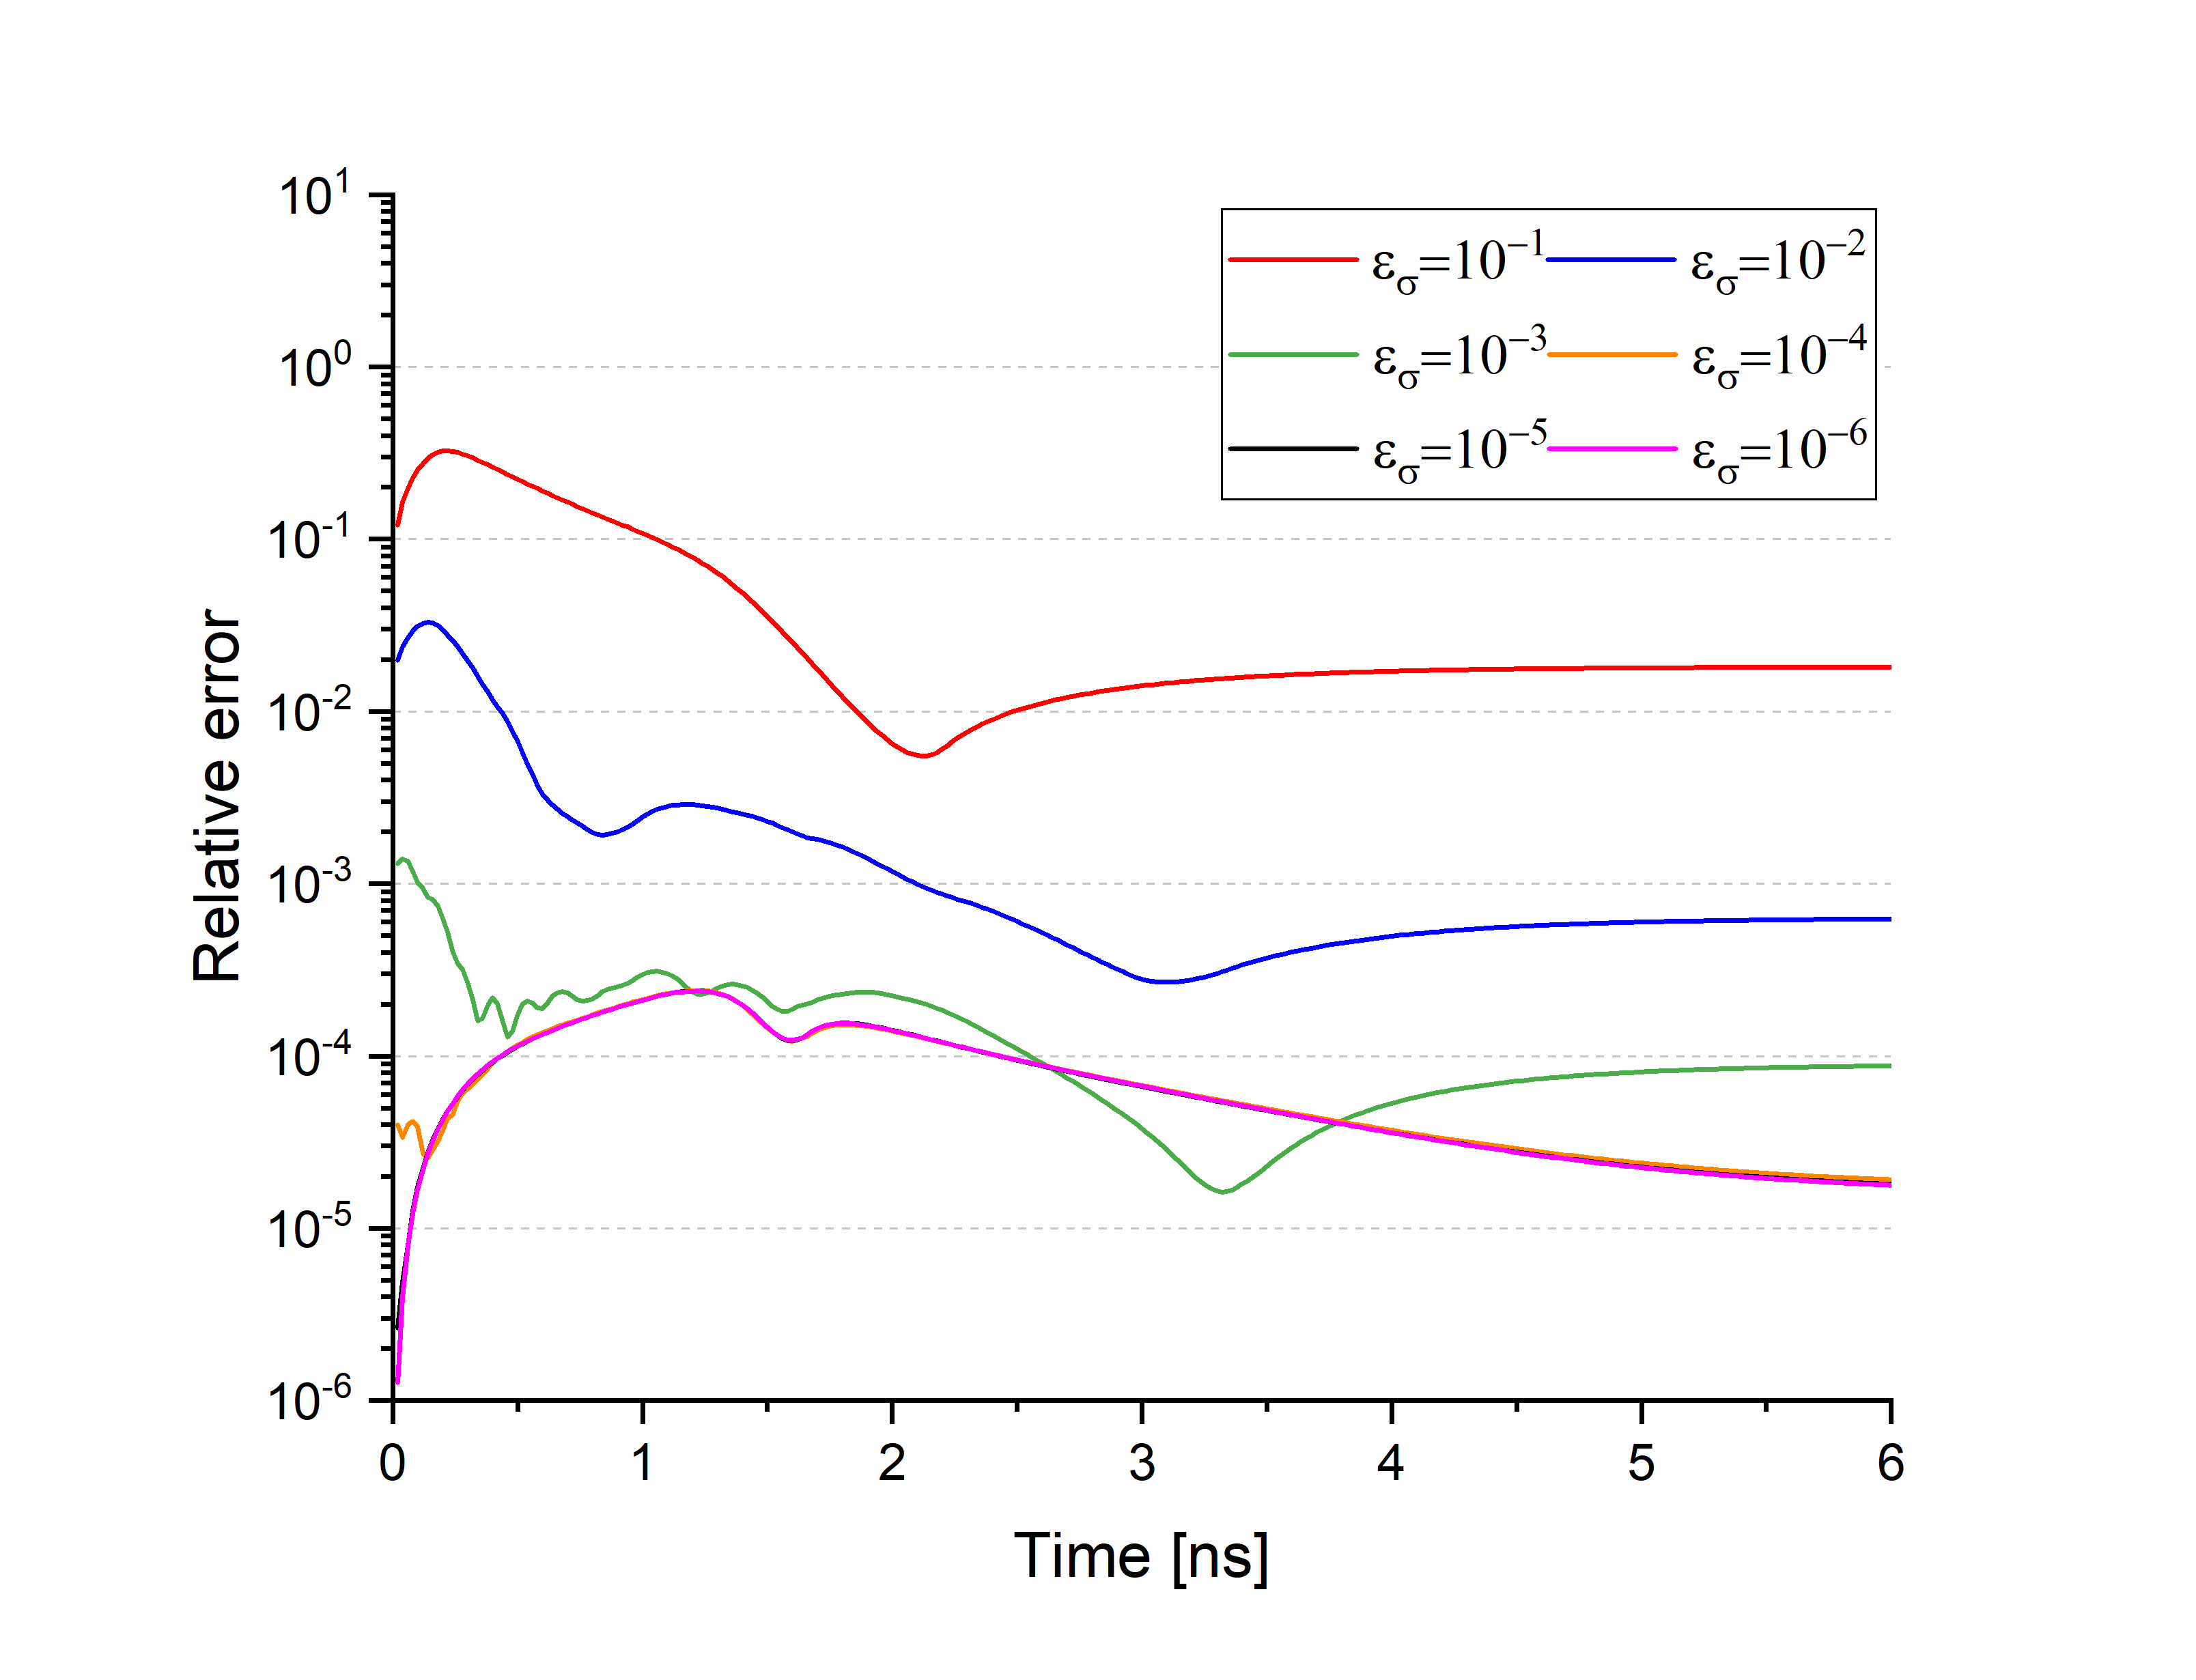
\includegraphics[width=0.5\textwidth]{MG_bc960-t002_qdf1000-920-t002_Tavg_mlqd.png}}
		\subfloat[Energy density relative error \label{subfig:MG_bc960-t002_qdf1000-920-t002_Eavg_mlqd}]{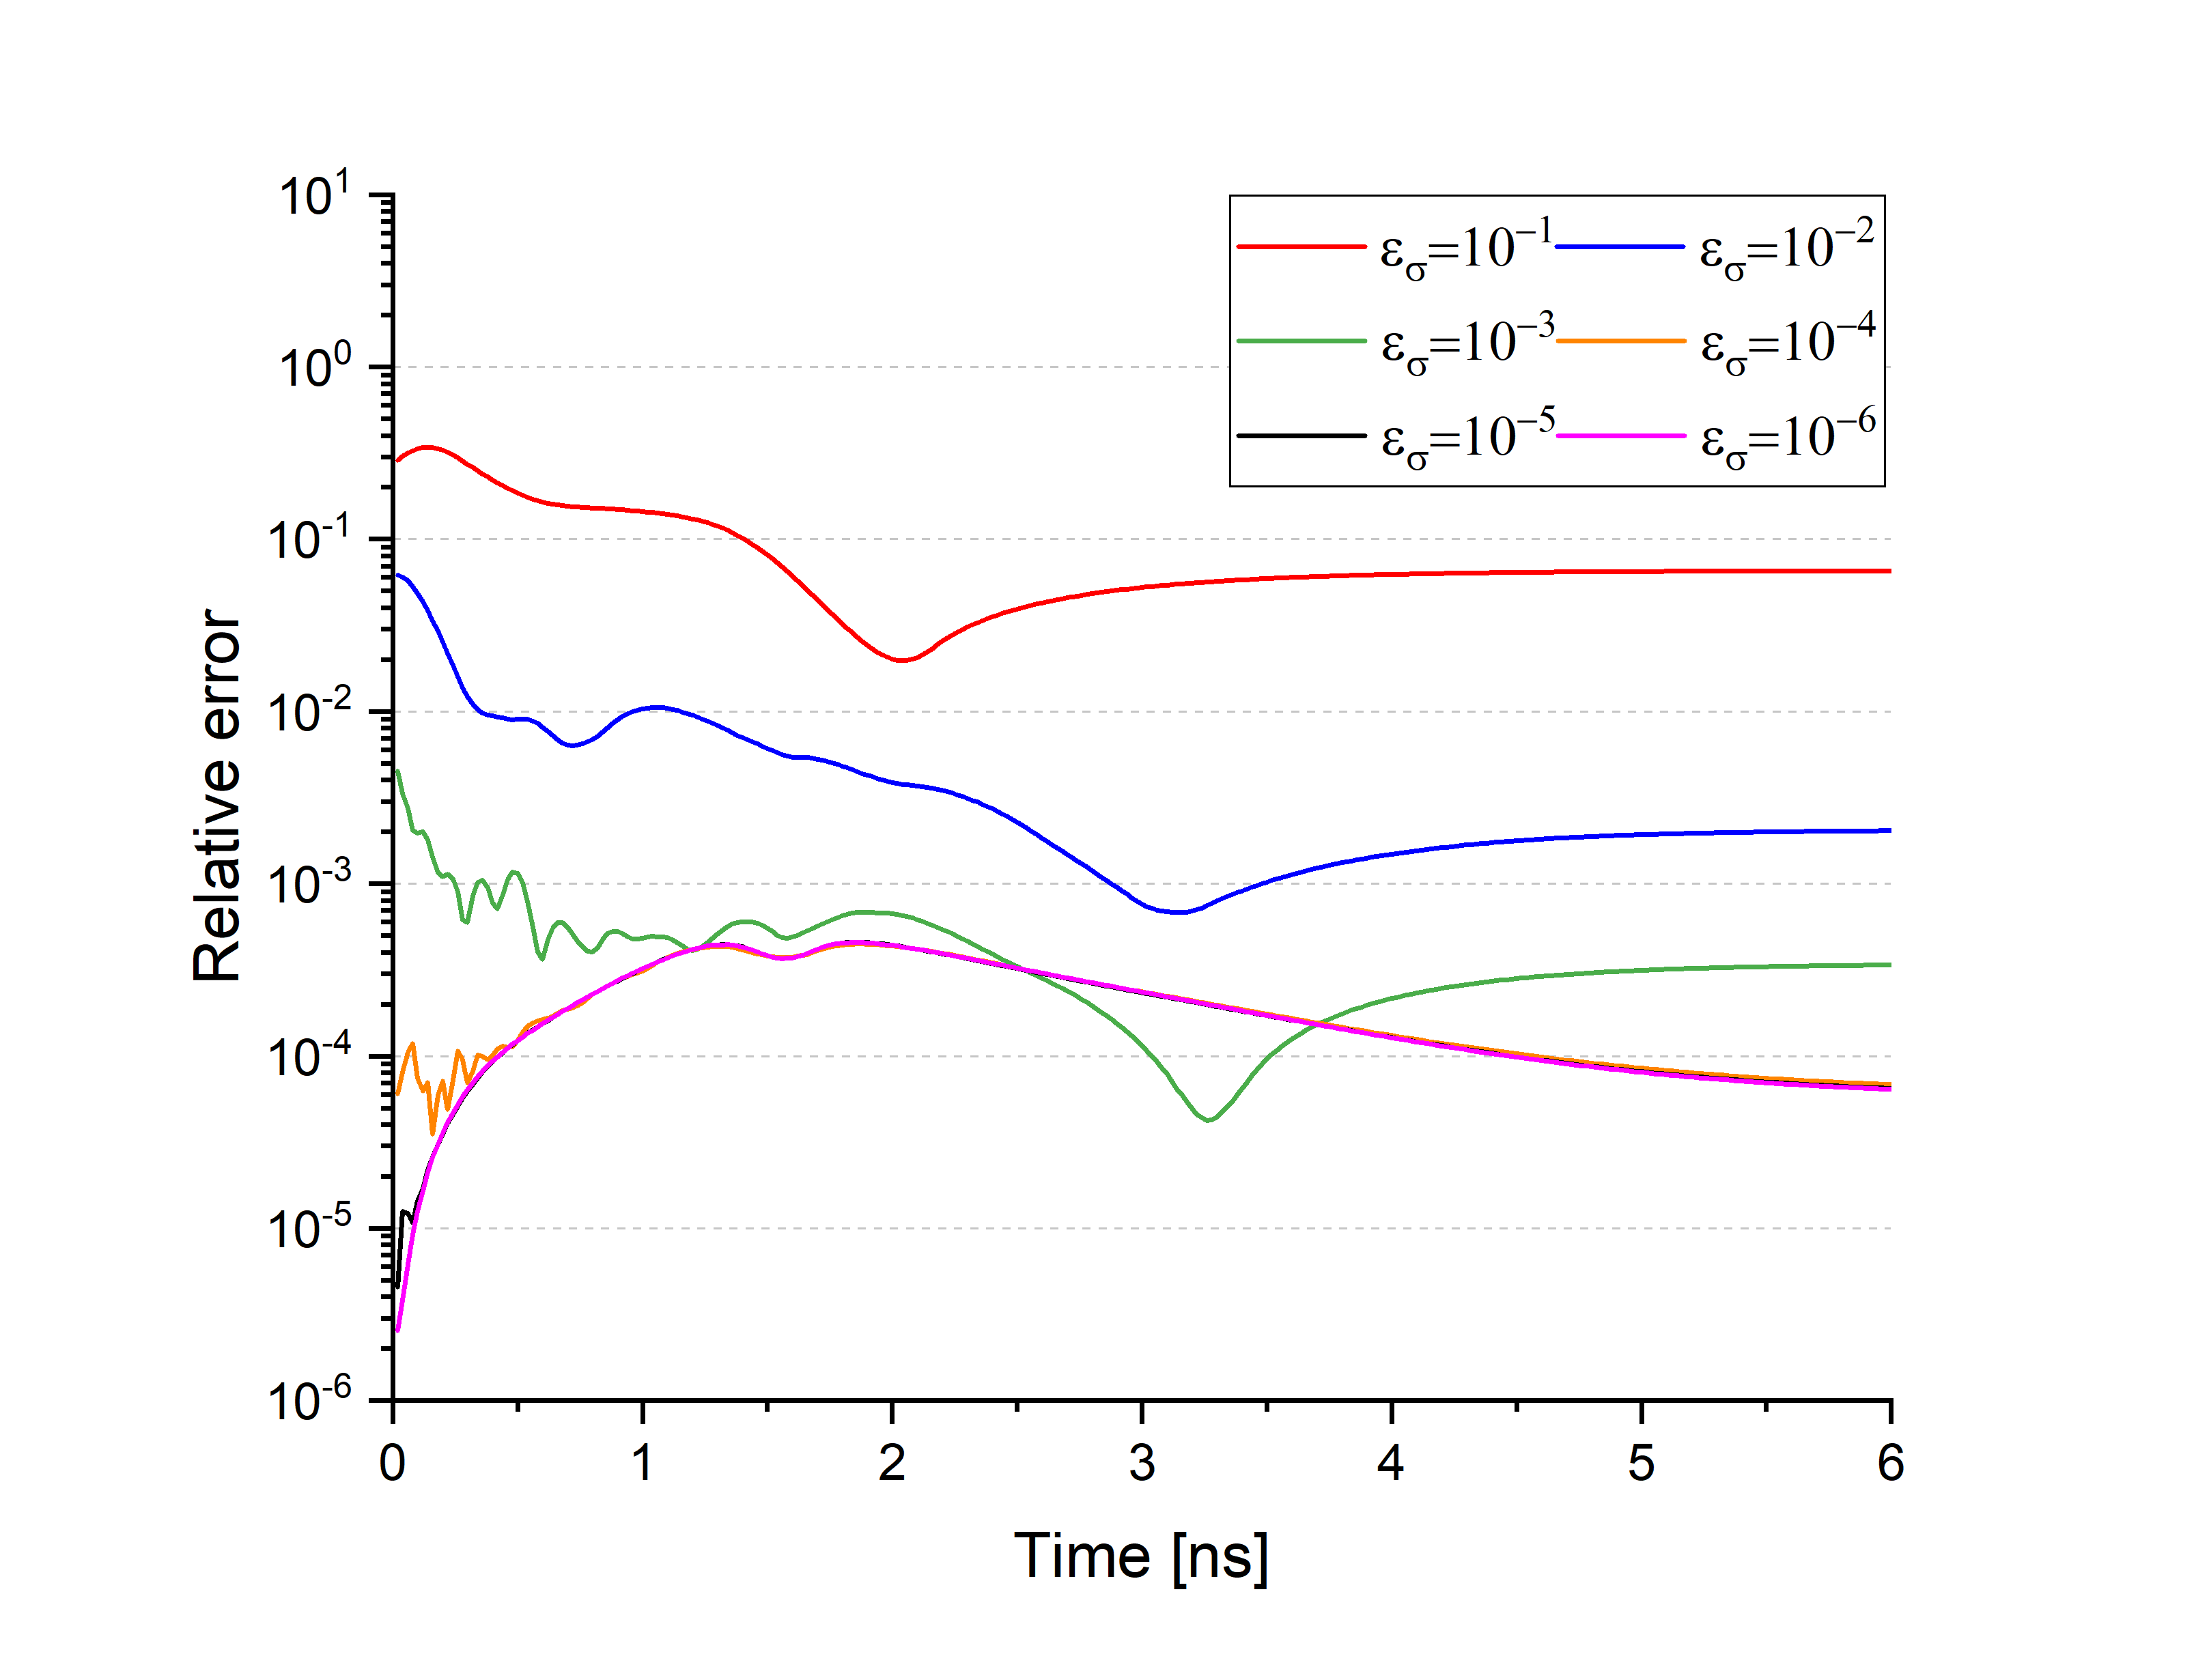
\includegraphics[width=0.5\textwidth]{MG_bc960-t002_qdf1000-920-t002_Eavg_mlqd.png}}
		\caption{\label{fig:errors_bc_T=960}
			Relative error in the $L_1$-norm of the MLOQD-POD ROM solutions computed with $T_{in}~=~0.96$~KeV using base cases with $T_{in}^{\pr{1}}=1$ KeV  and $T_{in}^{\pr{2}}=0.92$ KeV.}
	\end{figure}

	\ind The two types of ROMs utilizing an incomplete database can be combined to create a parameterized ROM with respect to the temperature $T_{in}$ of incoming radiation at the left boundary that also employs a reduced time step relative to the used database. In this case the same databases as created for the parameterized ROM in $T_{in}$ are adopted, now also interpolated linearly between instants of time. The first model uses $T_{in}^{(1)}~=~1$~KeV and $T_{in}^{(2)}=0.98$ KeV. The second one is formed with  $T_{in}^{(1)}=1$ KeV and $T_{in}^{(2)}=0.96$ KeV. The third is formed with  $T_{in}^{(1)}=1$ KeV and $T_{in}^{(2)}=0.92$ KeV. The data is generated for $\Delta t = 2\times10^{-2}$ ns. Figure \ref{fig:errors_bc_T=990_t001} shows the relative error in $L_1$-norm in the MLOQD-POD ROM solution  for $T_{in}=0.99$ KeV and $\Delta t = \! 1\! \times\! 10^{-2}$ ns computed by means of the first model with various values of $\varepsilon_{\sigma}$. Figure \ref{fig:errors_bc_T=980_t001} presents the relative error of the MLOQD-POD ROM solution for $T_{in}= 0.98$ KeV and $\Delta t = \! 1\! \times\! 10^{-2}$ ns obtained from the second model that is parameterized with a larger interval of $[T_{in}^{(1)},T_{in}^{(2)}]$. Figure \ref{fig:errors_bc_T=960_t001} presents the relative error of the MLOQD-POD ROM solution  for $T_{in}= 0.96$ KeV and $\Delta t = \! 1\! \times\! 10^{-2}$ ns obtained from the third model that is parameterized with the largest interval of  $[T_{in}^{(1)},T_{in}^{(2)}]$. The reference MLQD solution is recomputed for each $T_{in}$ at $\Delta t = \! 1\! \times\! 10^{-2}$ ns to find relative errors. The errors shown in Figs. \ref{fig:errors_bc_T=990_t001} - \ref{fig:errors_bc_T=960_t001} are very similar to Fig. \ref{fig:errors_dt-0.01}, and the error only marginally changes as the distance $[T_{in}^{(1)},T_{in}^{(2)}]$ is increased. This result demonstrates that these ROMs are most limited in accuracy by the refinement of time step length relative to the database of QD factors.

	%=================================================================================
	% BOUNDARY CONDITION DATABASE ERRORS PLOT	
	\begin{figure}[ht!]
		\centering
		\subfloat[Temperature relative error \label{subfig:MG_bc990-t001_qdf1000-980-t002_Tavg_mlqd}]{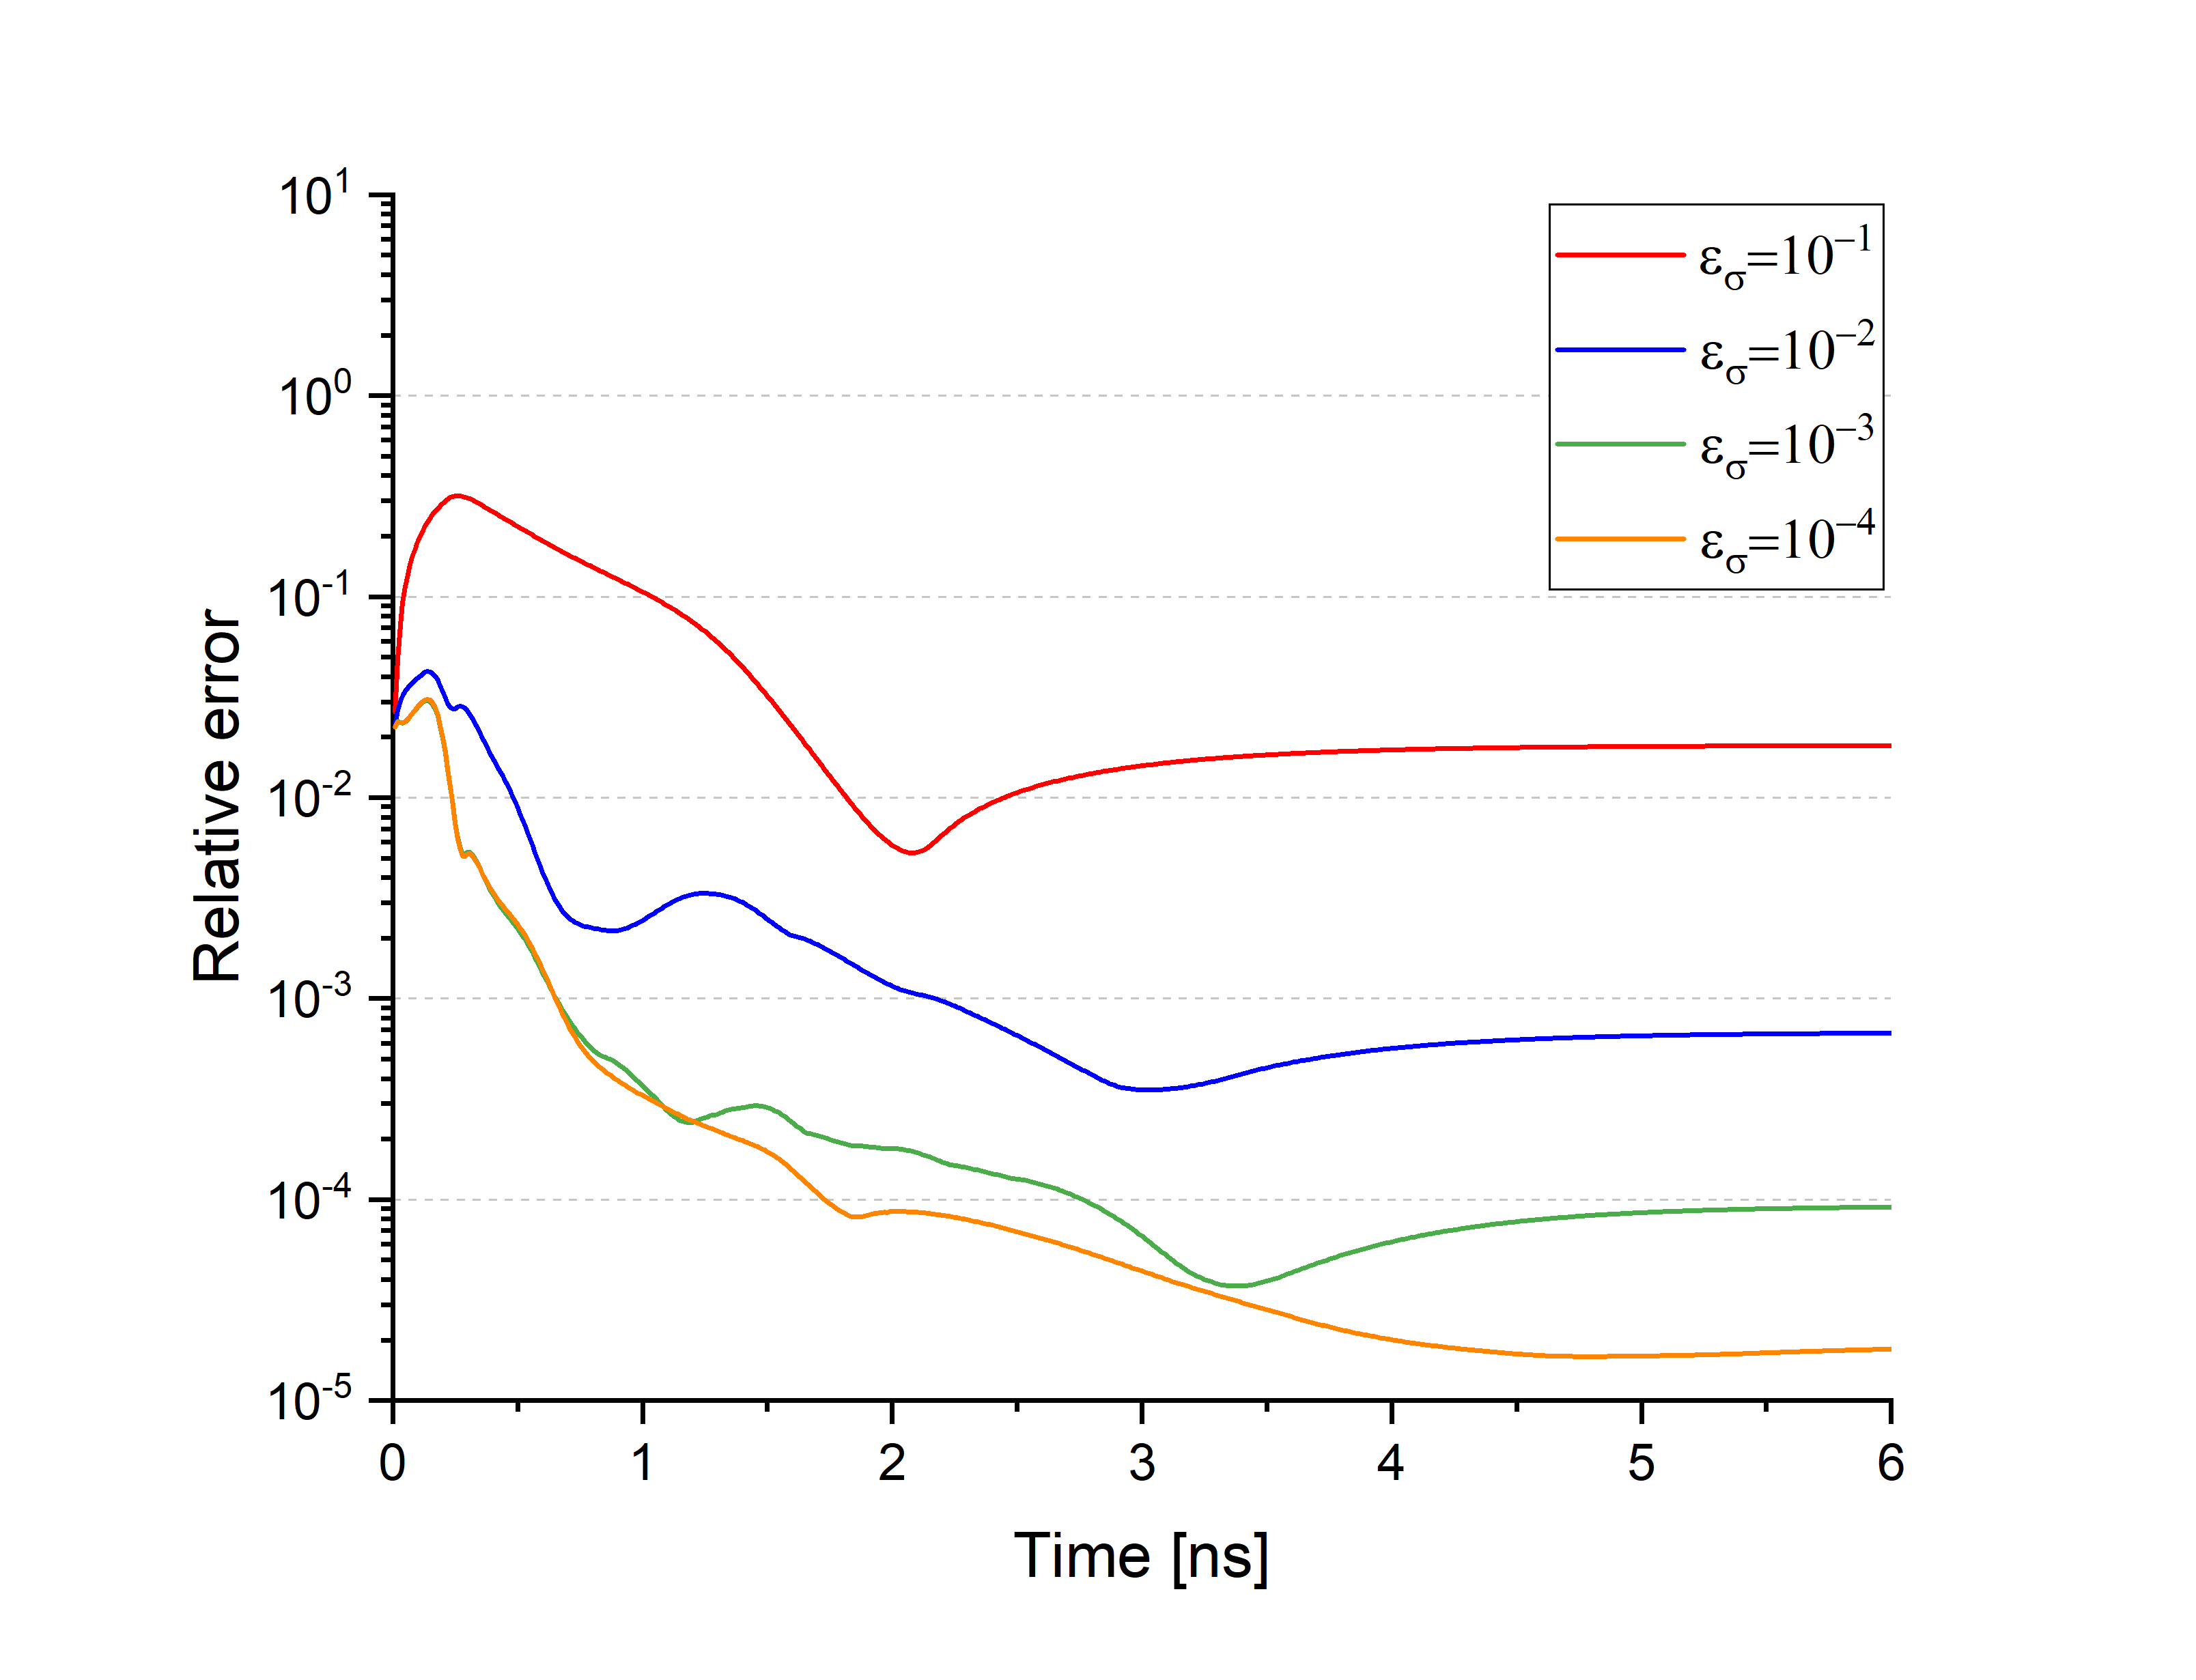
\includegraphics[width=0.5\textwidth]{MG_bc990-t001_qdf1000-980-t002_Tavg_mlqd.png}}
		\subfloat[Energy density relative error \label{subfig:MG_bc990-t001_qdf1000-980-t002_Eavg_mlqd}]{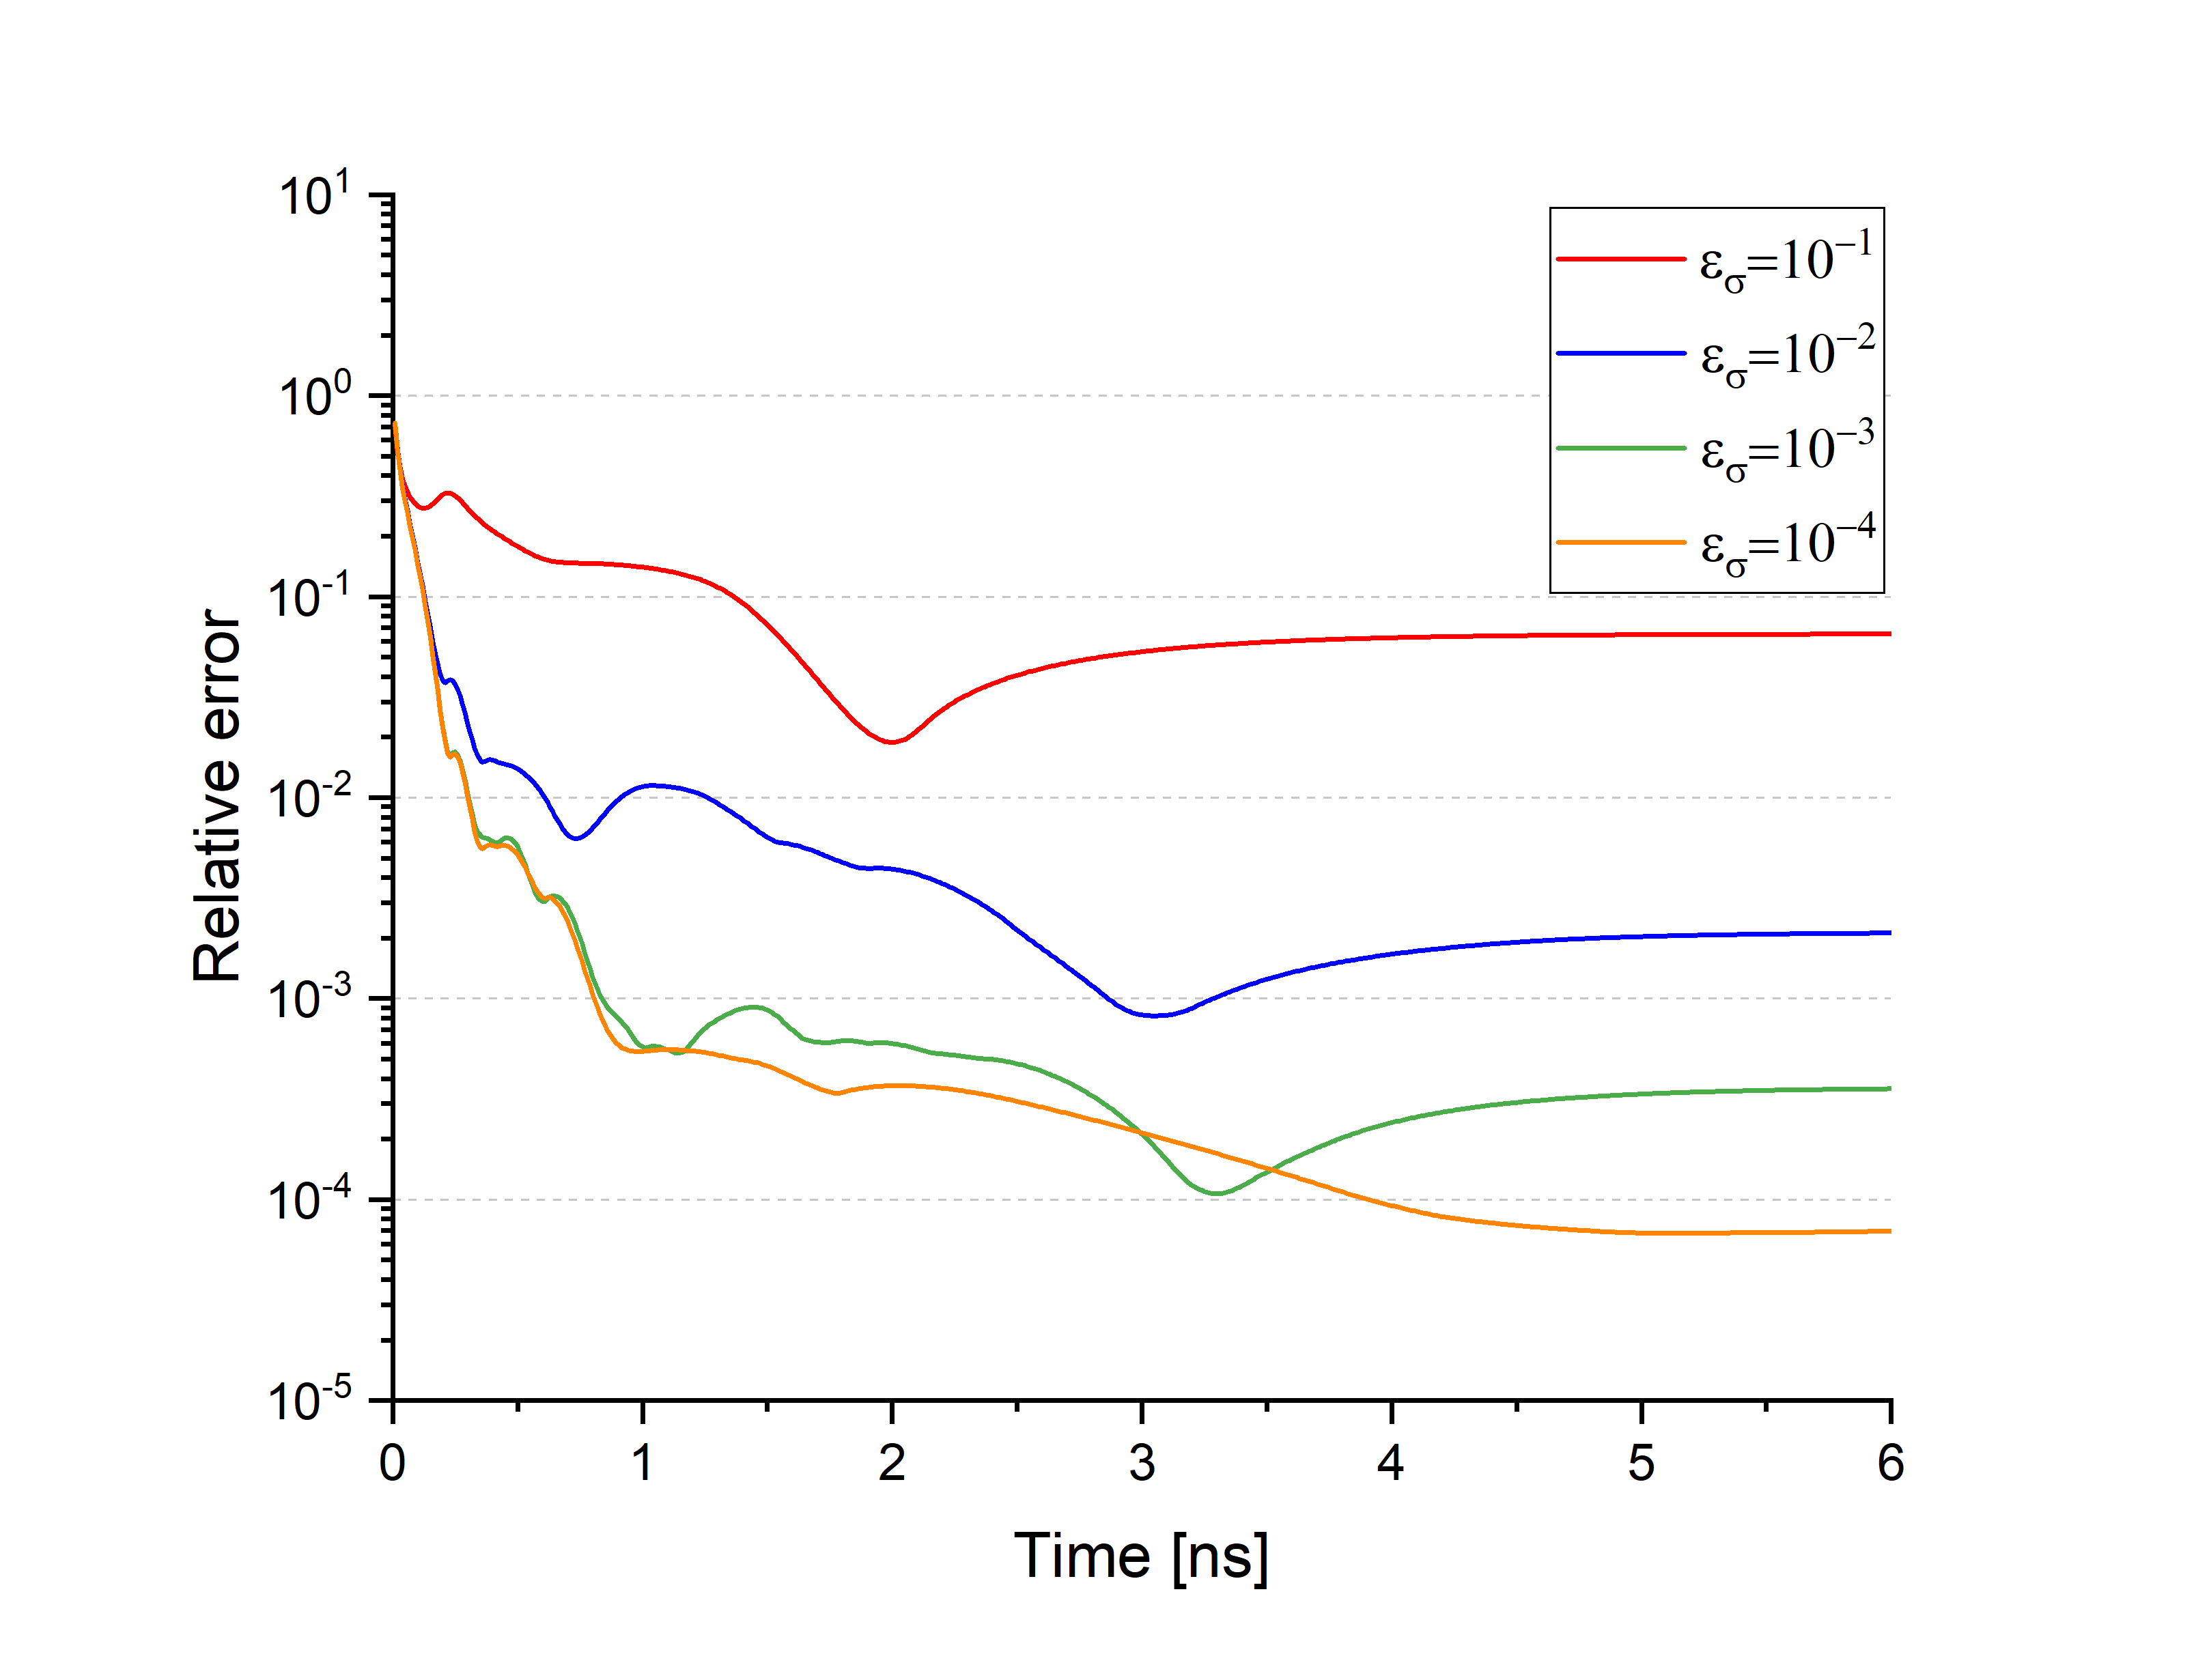
\includegraphics[width=0.5\textwidth]{MG_bc990-t001_qdf1000-980-t002_Eavg_mlqd.png}}
		\caption{\label{fig:errors_bc_T=990_t001}
			Relative error in the $L_1$-norm of the MLQD-POD solutions computed with $T_{in}~=~0.99$~KeV and $\Delta t\! =\! 1 \! \times \! 10^{-2}$~ns using base cases with $T_{in}^{\pr{1}}=1$ KeV  and $T_{in}^{\pr{2}}=0.98$ KeV and $\Delta t\! =\! 2 \! \times\!  10^{-2}$.}
	\end{figure}

	\begin{figure}[ht!]
		\centering
		\subfloat[Temperature relative error \label{subfig:MG_bc980-t001_qdf1000-960-t002_Tavg_mlqd}]{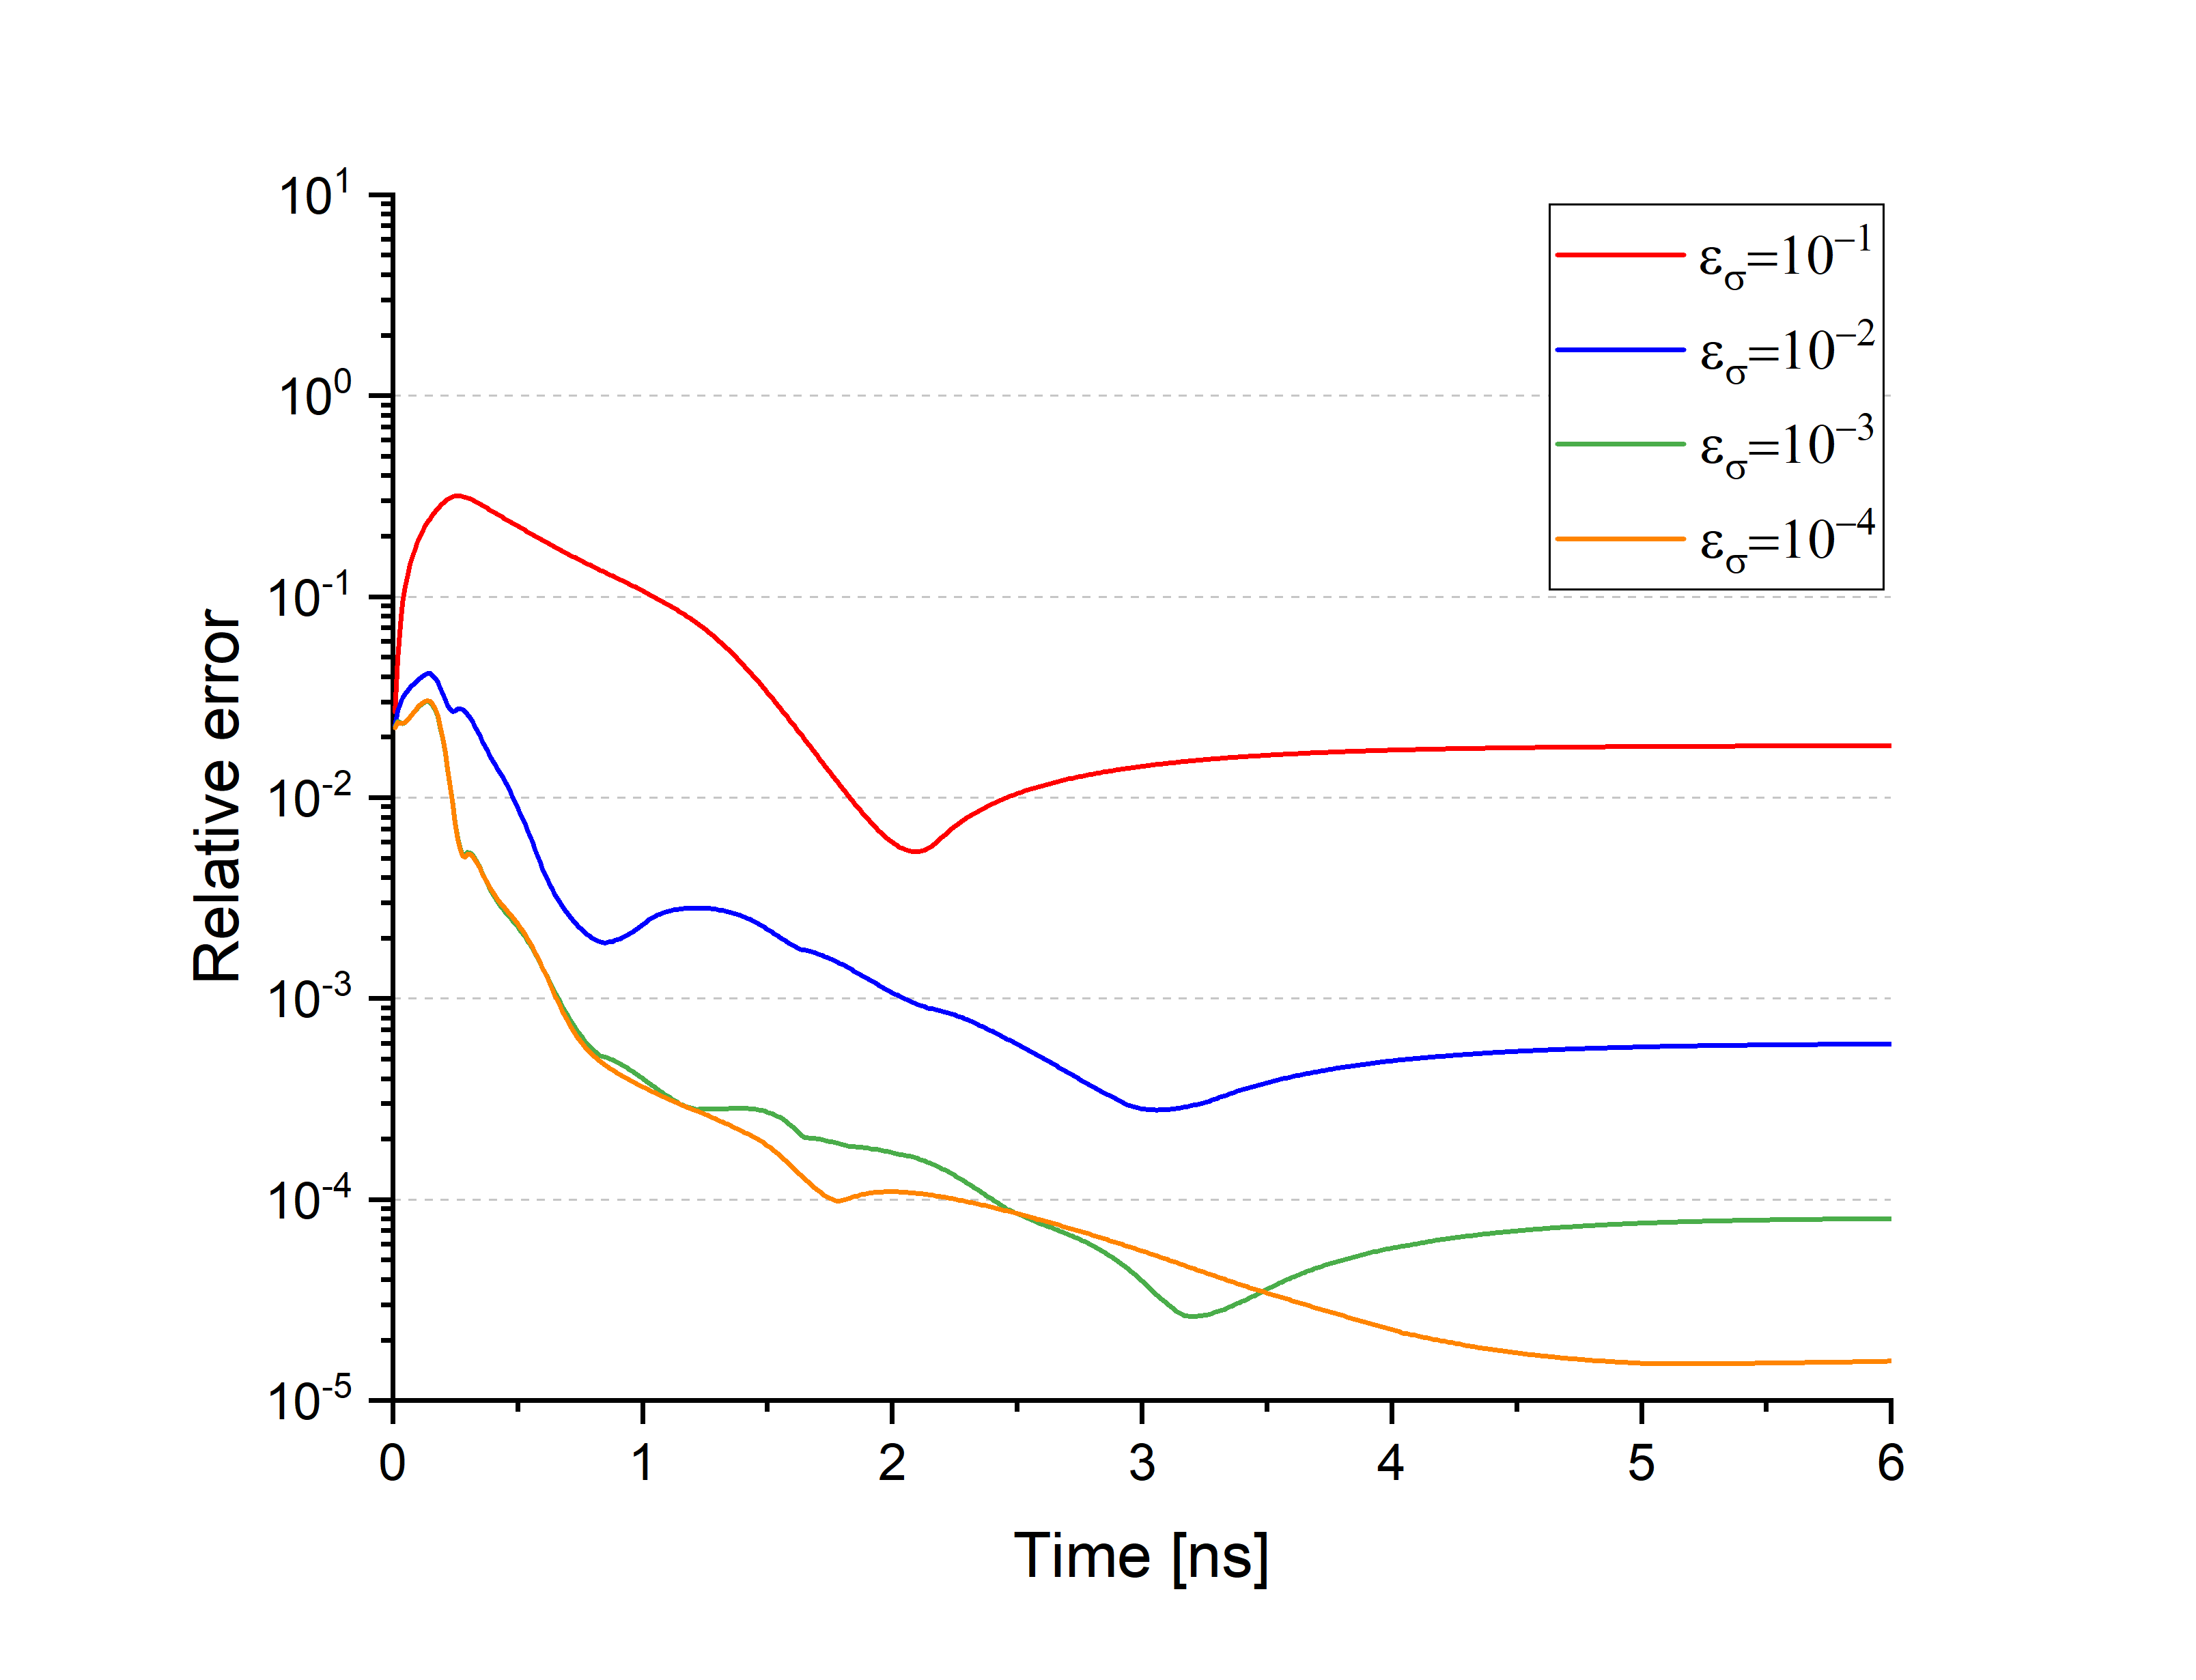
\includegraphics[width=0.5\textwidth]{MG_bc980-t001_qdf1000-960-t002_Tavg_mlqd.png}}
		\subfloat[Energy density relative error \label{subfig:MG_bc980-t001_qdf1000-960-t002_Eavg_mlqd}]{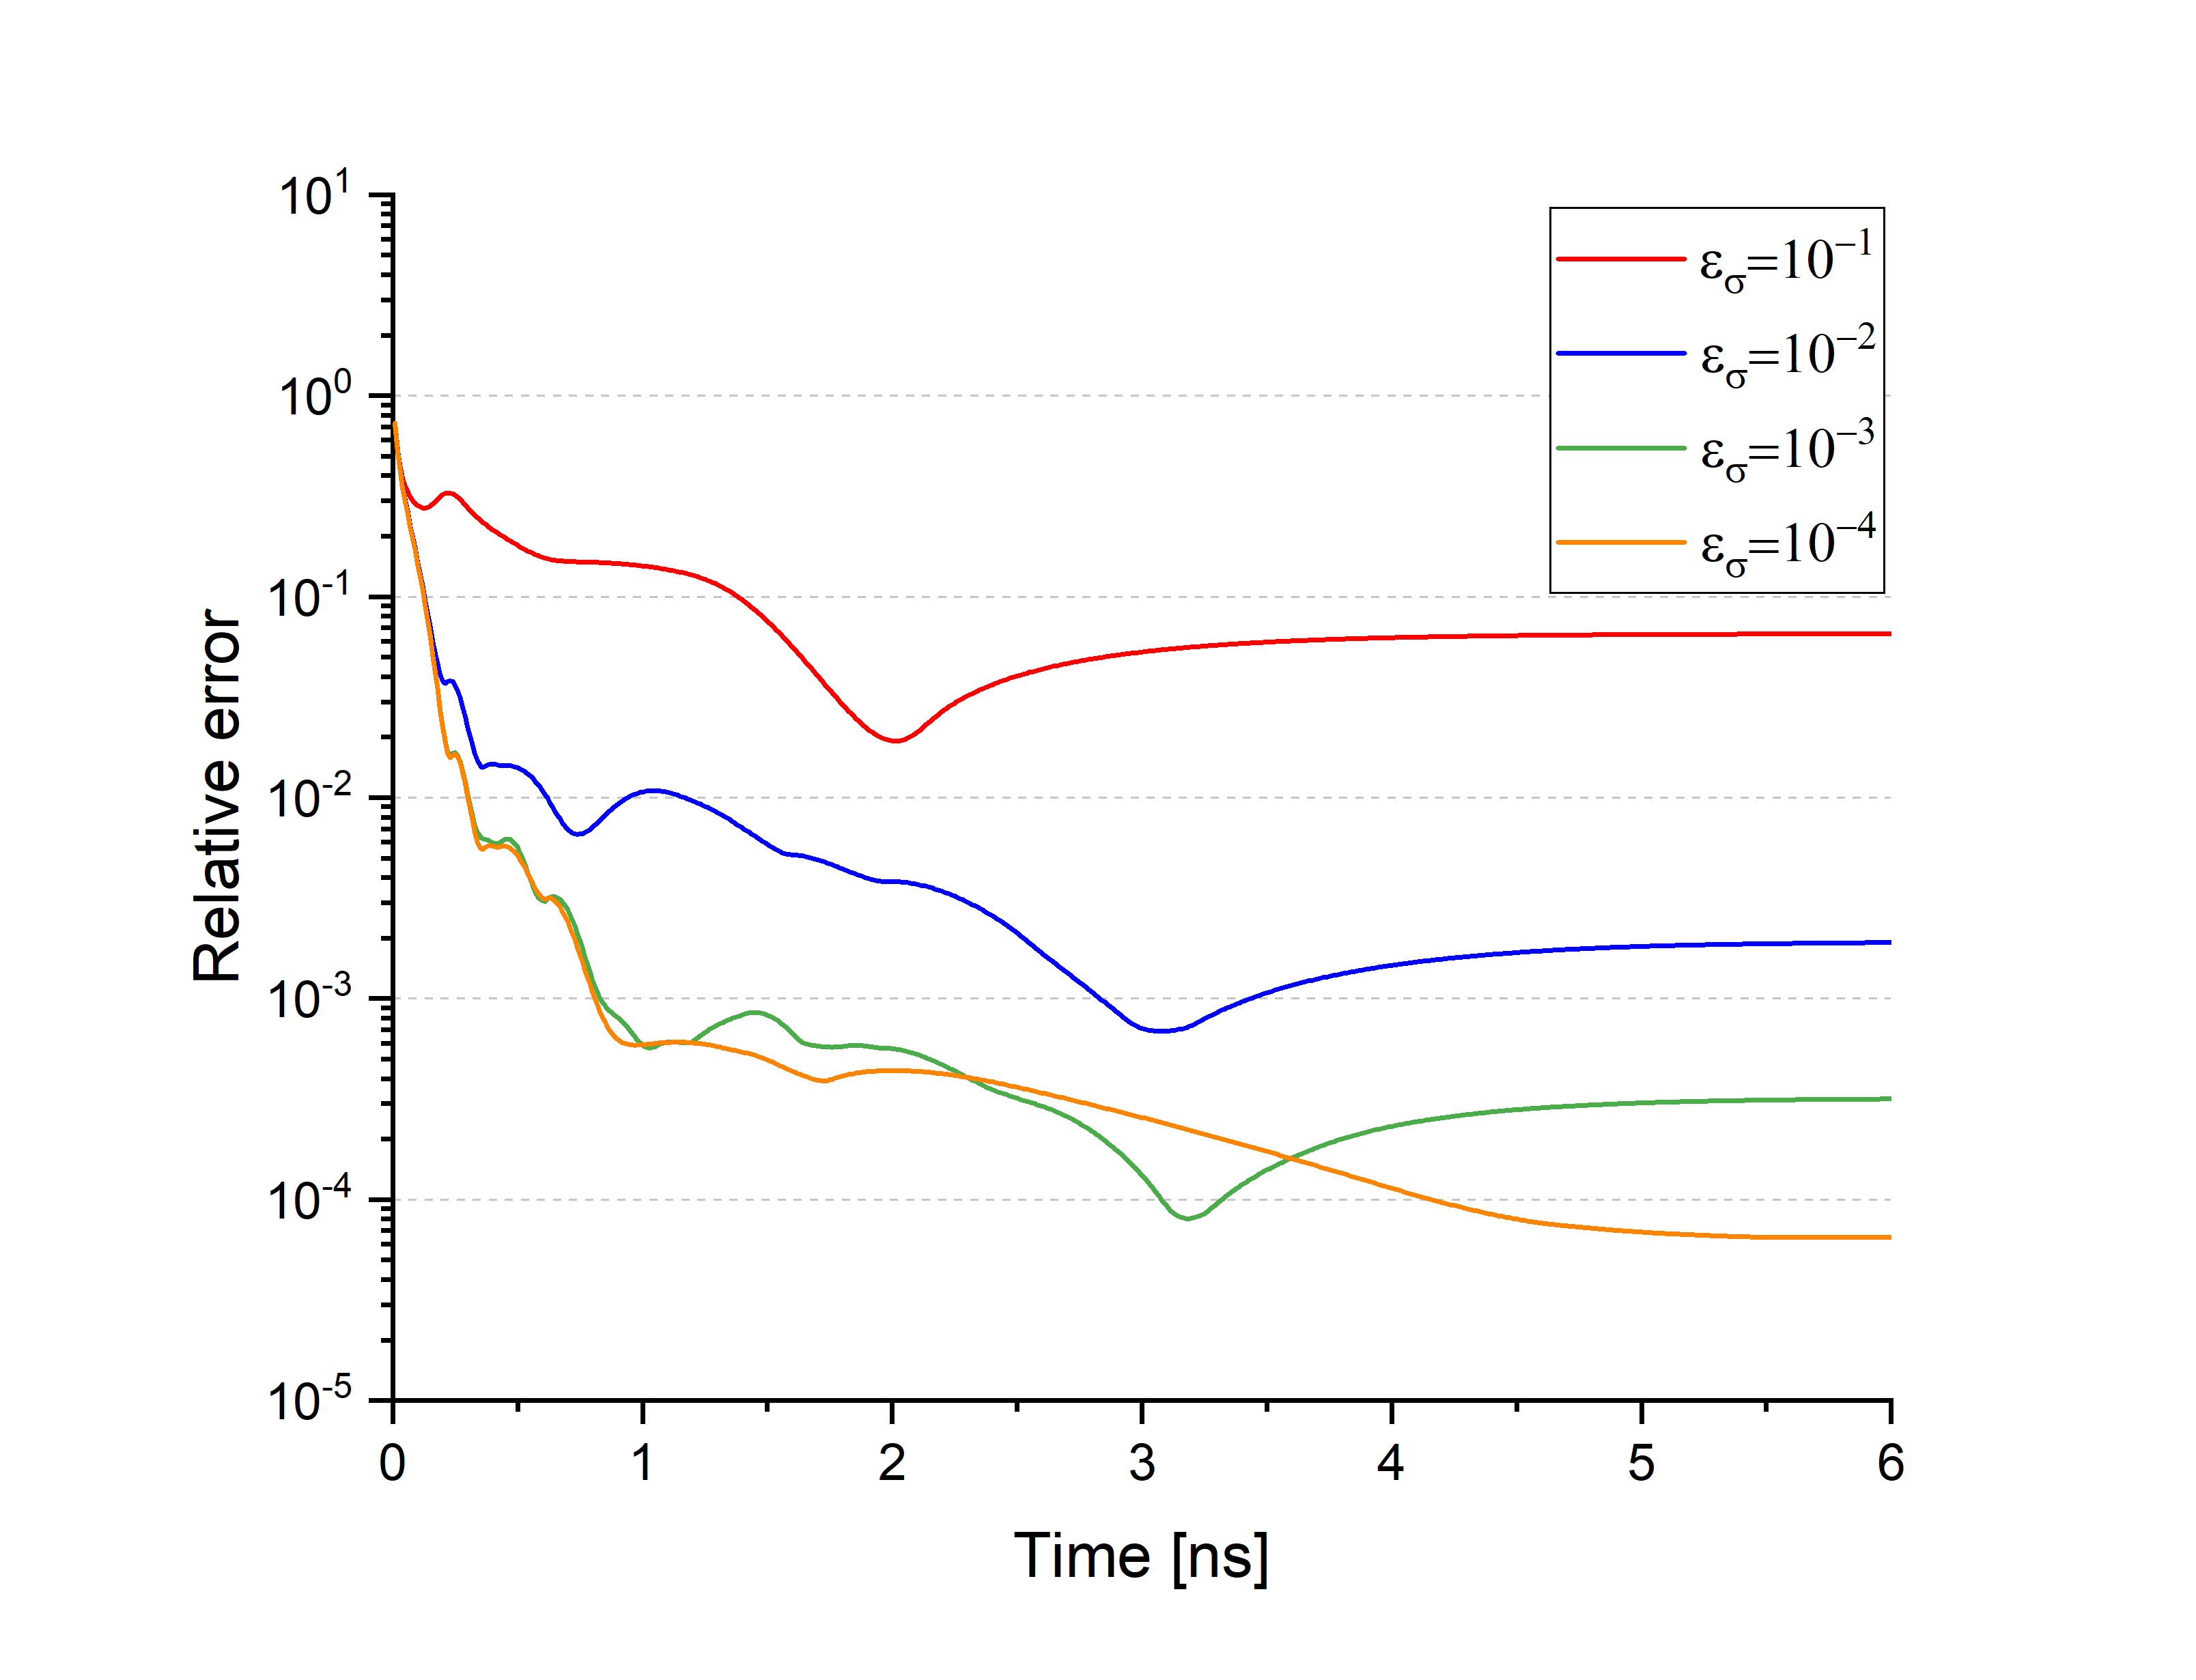
\includegraphics[width=0.5\textwidth]{MG_bc980-t001_qdf1000-960-t002_Eavg_mlqd.png}}
		\caption{\label{fig:errors_bc_T=980_t001}
			Relative error in the $L_1$-norm of the MLQD-POD solutions computed with $T_{in}~=~0.98$~KeV and $\Delta t\! =\! 1 \! \times \! 10^{-2}$~ns using base cases with $T_{in}^{\pr{1}}=1$ KeV  and $T_{in}^{\pr{2}}=0.96$ KeV and $\Delta t\! =\! 2 \! \times\!  10^{-2}$.}
	\end{figure}

	\begin{figure}[ht!]
		\centering
		\subfloat[Temperature relative error \label{subfig:MG_bc960-t001_qdf1000-920-t002_Tavg_mlqd}]{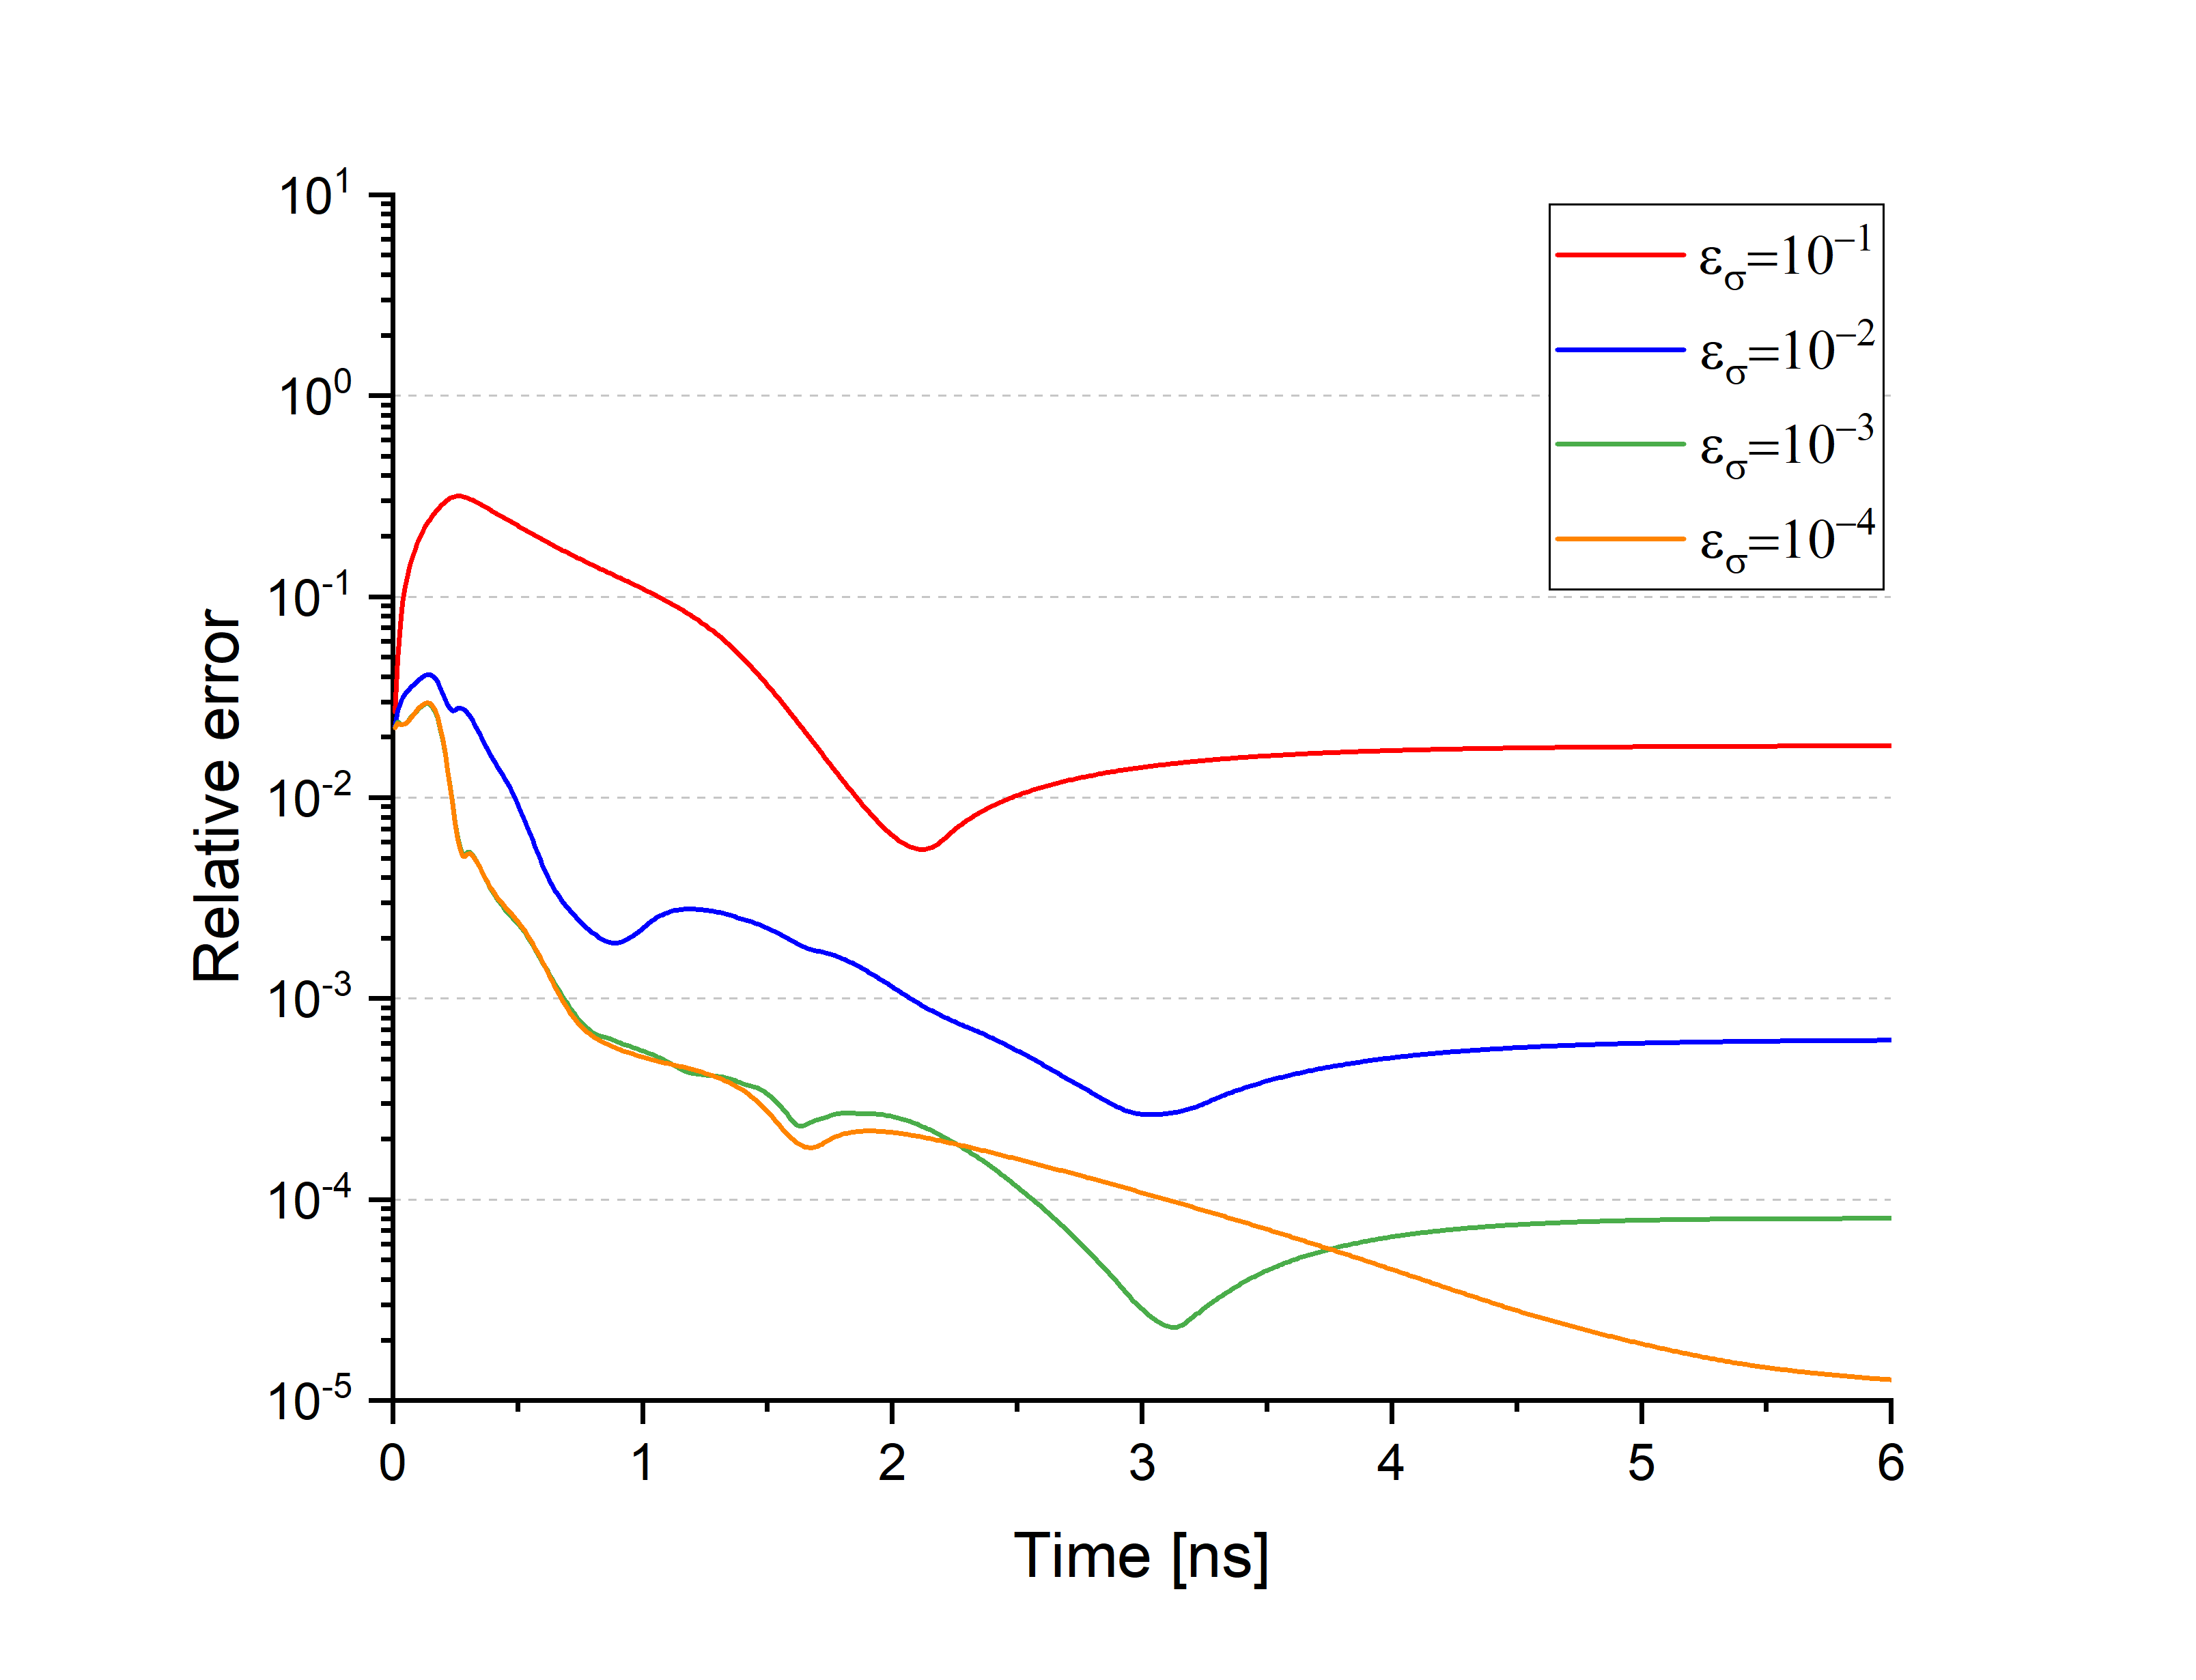
\includegraphics[width=0.5\textwidth]{MG_bc960-t001_qdf1000-920-t002_Tavg_mlqd.png}}
		\subfloat[Energy density relative error \label{subfig:MG_bc960-t001_qdf1000-920-t002_Eavg_mlqd}]{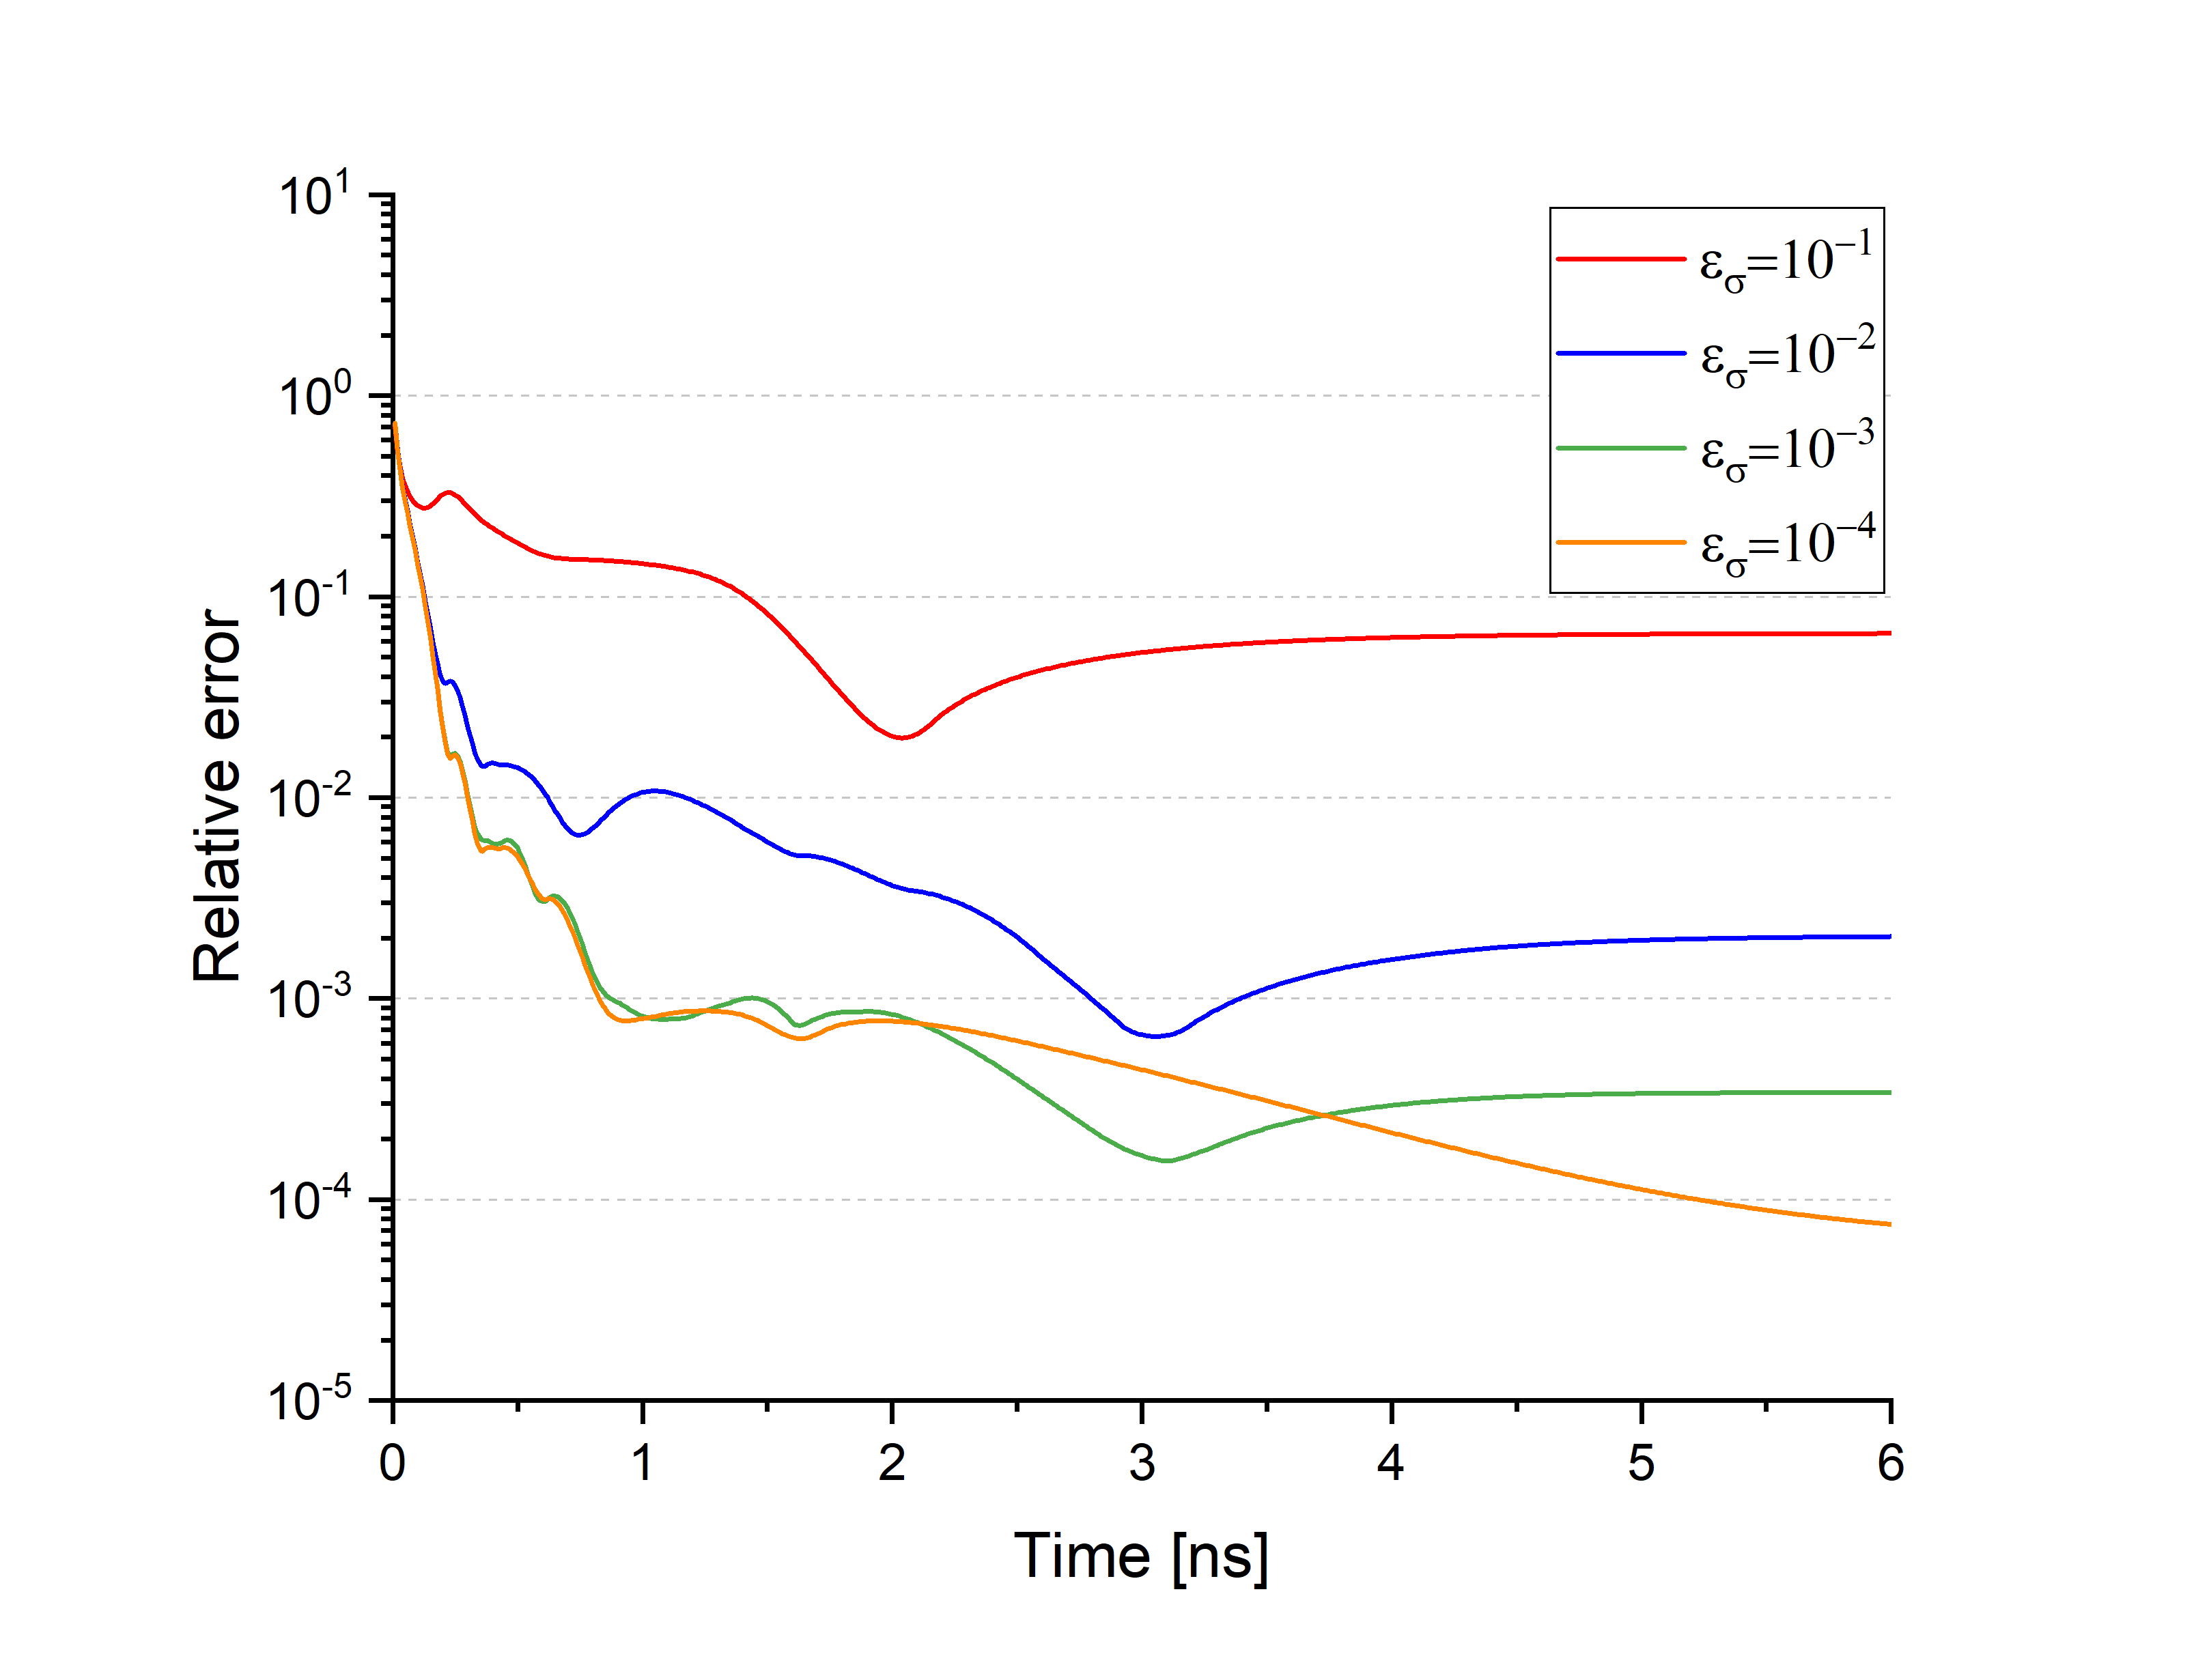
\includegraphics[width=0.5\textwidth]{MG_bc960-t001_qdf1000-920-t002_Eavg_mlqd.png}}
		\caption{\label{fig:errors_bc_T=960_t001}
			Relative error in the $L_1$-norm of the MLQD-POD solutions computed with $T_{in}~=~0.96$~KeV and $\Delta t\! =\! 1 \! \times \! 10^{-2}$~ns using base cases with $T_{in}^{\pr{1}}=1$ KeV  and $T_{in}^{\pr{2}}=0.92$ KeV and $\Delta t\! =\! 2 \! \times\!  10^{-2}$.}
	\end{figure}

